%-----------------------------------------------------------------------
% Latex Thesis/Dissertation Template for Wright State University
% 
% Written by Sean A. Mortara
% 28 June 2001
% Modified by Josh Mark
% 15 Dec 2011
% Later edits by Joseph C. Slater
%-----------------------------------------------------------------------
\documentclass[12pt]{report}

\usepackage{xcolor}
\usepackage{booktabs} % used for tables
\usepackage{multirow} % used for tables to merge multiple rows
\usepackage{bigdelim} % used for tables to set spacing
\usepackage{bigstrut} % used for tables to set spacing
\usepackage{graphicx} % used for includegraphics
\usepackage{subfigure} % allows the use of subfigures
\usepackage{amssymb,amsmath} % For math
\usepackage{graphicx, float, subfigure, caption} % For figures
\usepackage[framed,numbered,autolinebreaks,useliterate]{mcode} % used to insert code
%
\usepackage[hidelinks]{hyperref}
\usepackage{xcolor}
\hypersetup{
    colorlinks,
    linkcolor={blue!50!black},
    citecolor={blue!50!black},
    urlcolor={blue!80!black}
}
%-----------------------------------------------------------------------
%  Modified fields
%-----------------------------------------------------------------------
\newcommand{\authorfirst}{Koorosh}
\newcommand{\authorMI}{}
\newcommand{\authorlast}{Gobal}
\newcommand{\degreefull}{Doctor of Philosophy}  % force hyphenation at syllables if line breaks are required
\newcommand{\degreeshort}{Ph.D.}
\newcommand{\thesisordissertationlc}{Dissertation}
\newcommand{\dept}{Department of Mechanical Engineering}
\newcommand{\institution}{Wright State University} % Doubting you will
                                % change this. 
\newcommand{\thesistitle}{High-Fidelity Multidisciplinary Sensitivity Analysis for Coupled Fluid-Solid Interaction Design} % Needes a line break
\newcommand{\bachdegreeshort}{B.S.M.E.} % Bachelor degree short
\newcommand{\bachinstitution}{Sharif University of Technology} % Bachelor degree institution
\newcommand{\bachyear}{2012}% Bachelor degree year
%No spaces should be before or after this title.
\newcommand{\pdfsubject}{Shape Sensitivity Analysis for FSI Design}
\newcommand{\pdfkeywords}{Sensitivity Analysis, Fluid-Solid Interaction, Multidisciplinary Design Optimization}
\newcommand{\yearcomplete}{2016}
% set pdf file info
\usepackage{hyperxmp} % used to set pdf property info with \hypersetup command

%-----------------------------------------------------------------------
%  Thesis Advisor, Department Chair, Dean of Graduate Studies
%  I don't know why titles as separated... except in the one case at
%  the end. 
%-----------------------------------------------------------------------
\newcommand{\thesisdirector}{Ramana V. Grandhi}
\newcommand{\thesisdirectortitle}{Ph.D.}
\newcommand{\phdProgrameChair}{Frank W. Ciarallo}
\newcommand{\phdProgrameChairTitle}{Ph.D.}
\newcommand{\graduateSchoolDean}{Robert E.W. Fyffe}
\newcommand{\graduateSchoolDeanEducation}{Ph.D.}
\newcommand{\graduateSchoolDeanTitle}{Vice President for Research and \\Dean of the Graduate School}
%-----------------------------------------------------------------------
%  Final Examination Committee: Comment out the ones you don't need. 
%-----------------------------------------------------------------------
\newcommand{\fecone}{Ramana V. Grandhi, Ph.D.}

\newcommand{\fectwo}{Mitch Wolff, Ph.D.}

\newcommand{\fecthree}{Ha-Rok Bae, Ph.D.}

\newcommand{\fecfour}{Robert A. Canfield, Ph.D.}

\newcommand{\fecfive}{Raymond M. Kolonay, Ph.D.}

\newcommand{\fecsix}{Christopher M. Koehler, Ph.D.}

% If you have more committee members... good luck

% Modify this if needed for getting citations to "look right" according to your field. Read the natbib documentation on how to use this. 
%\usepackage[round]{natbib}
%\usepackage{doublespace}

%=============================
%  Begin document!
%=============================
%
% Don't touch

% still don't touch.   

% title sheet
\usepackage{WSU}
%\hypersetup{
%                     pdfauthor={\authorfull},
%                     pdftitle={\thesistitle},
%                     pdfsubject={\pdfsubject},
%                     pdfkeywords={\pdfkeywords},
%                     }
% \normalem
\pagenumbering{roman}
\pagestyle{plain}
\rhead{\today}
\begin{document}
\maketitle
\doublespace

% Still don't touch!!

%=============================
%  approval sheet
%=============================

\thispagestyle{empty}
\renewcommand\baselinestretch{2}
\begin{singlespace}
\signaturepage
\end{singlespace}
%
%=============================
%  Abstract
%=============================
\newpage
\setcounter{page}{3}
\vspace{2in}
%
\begin{singlespace}
\begin{center}
  ABSTRACT
\end{center}
%
\noindent{\small{\authorlast, \authorfirst}. 
		 {\degreeshort, \dept, \institution}, 
		 {\yearcomplete}. 
		 {\sl \thesistitle}.}
\end{singlespace}
\vspace*{.5in}

\pdfbookmark[0]{Abstract}{Abstract}
%\phantomsection
%
%========================
% Start editing below. 
%========================
\begin{abstract}
In many engineering disciplines such as aerospace, marine, automotive, and biomedical engineering the consideration of the coupling between the fluid and structural systems are necessary for quality engineering analysis. Therefore, the need for such analysis in the design processes is continuously increasing. The primary motivation for this work is to develop a sensitivity analysis tool that is capable of calculating accurate sensitivities without significant modification of the source codes for simulations based on non-body conformal grids. The majority of work done on the coupled fluid-solid simulations are based on computational grids that conform to the solid boundaries. This becomes a restriction for complex boundary shapes or large deformation of the solid domain for these systems. The hurdles associated with the body-conformal techniques are mainly due to additional cost related to mesh deformation and the effect of mesh movement on sensitivity calculation. Therefore, we propose to use a particular family of non-body conformal techniques often known as Immersed Boundary (IB) methods for modeling the flow over immersed boundaries. The Continuum Sensitivity Analysis (CSA) is added on top of the IB method, which calculates the sensitivity of the flow variables, velocity and pressure. These variables are modeled with Navier-Stokes (NS) equations, and their sensitivities are calculated with respect to change in the shape of the solid boundary. This technique is implemented in the calculation of the sensitivity of the coupled fluid-structure system subject to different shape design variables. The sensitivity of various benchmark problems such as flow between parallel plates, over a cylinder, and through a convergent-divergent nozzle is calculated with respect to shape parameters using this approach. These results are verified using the complex step method which gives accurate sensitivities up to machine precision. This work is the first implementation of CSA for continuous IB method for viscous flow (Navier-Stokes) models.
\end{abstract}
%%%%%%%%%%%%%%%%%%
%-----------------------------------------------------------------------
%
%=============================
%  List of symbols (Optional)
%=============================
%\newpage
%%\renewcommand\baselinestretch{1.5}
%\begin{singlespace}\begin{center}
%  \textbf{\Huge{List of Symbols}}
%\end{center}
%
%\begin{flushleft}{\large Chapter 2} \end{flushleft}
%\begin{tabular}{p{0.75in}l}
%   $\gamma$ & $\frac{-b+\sqrt{b^{2}-4ac}}{2a}$\\
%   $L$ & {Plate length}\\
%\end{tabular}
%
%%%%%%
%\begin{flushleft}{\large Chapter 3} \end{flushleft}
%\begin{tabular}{p{0.75in}l}
%   $h$ & {Plate thickness}\\
%   $L$ & {Plate length}\\
%\end{tabular}
%
%%%%%%
%\begin{flushleft}{\large Chapter 4} \end{flushleft}
%\begin{tabular}{p{0.75in}l}
%   $M_{\infty}$ & {Freestream Mach number}\\
%   $U_{\infty}$ & {Freestream fluid velocity}\\
%   $p-p_\infty$ & {Aerodynamic pressure differential}\\
%\end{tabular}
%
%%%%%%
%\begin{flushleft} {\large Chapter 7} \end{flushleft}
%\begin{tabular}{p{0.75in}l}
%   $\beta$   & $\sqrt{M_{\infty}^2-1}$\\
%   $\lambda$ & {Nondimensional freestream dynamic pressure}\\
%\end{tabular}
%\end{singlespace}
%=============================
%  Table of contents, etc.
%=============================
%\renewcommand\baselinestretch{1.5}
\begin{singlespace}
\tableofcontents
\listoffigures
\listoftables
\end{singlespace}
%
%=============================
%  Acknowledgments
%=============================
\newpage
\thispagestyle{plain}
\setlength{\parindent}{0em}
\begin{center}
{\huge Acknowledgment}
\end{center}

%I would like to take this opportunity to extend my thanks to\ldots If you have multiple paragraphs, the first should not be indented to match the style of the rest of the thesis
%
%\setlength{\parindent}{2em}
%Any additional paragraphs should be indented as such.  Remember to thank your advisor and committee members.
%
%=============================
%  Dedication
%=============================
%\newpage
%\thispagestyle{plain}
%\vspace*{3in}
%\begin{center}
%Dedicated to\\
%Somebody special (Wife, husband, girlfriend or boyfriend works well
%here. )
%\end{center}
%
%
%
%=============================
%  Begin Chapters
%=============================
\newpage
\setcounter{page}{1}
\pagenumbering{arabic}
\setlength{\parindent}{2em}
%=============================
%
\chapter{Introduction}\label{ch:introduction}
% ======================================================================================
\section{Motivation}
Fluid-structure interaction (FSI) problems play an important role in many scientific and engineering fields, such as automotive, aerospace, and biomedical industry. Despite the wide application, a comprehensive study of FSI systems still remains a challenge due to their strong nonlinearity and multi-physics nature. For most FSI problems, analytical solutions of responses are not available and physical experiments are limited in scope, expensive to conduct, and are time consuming. Therefore, in order to get more insight in the physics involved in the complex interaction between fluids and solids, numerical simulations are typically used. The numerical solutions are conducted using Computational Fluid Dynamics (CFD) models for the flow field and Finite Element Analysis (FEA) for the structural response. Nevertheless, the prohibitive amount of computations has been one of the major issues in the design optimization of such coupled multidisciplinary systems. The other bottle neck is generating an appropriate computational domain that represents the fluid and solid regions with desired fidelity. The effort and time required to take a geometry from a CAD package, refining the model and generating a computational mesh is usually a large portion of the overall human time required for the simulation. This cannot be automated easily for complex and moving domains. Therefore, techniques that decouple the mesh topology from the shape of the solid boundary can drastically simplify the simulation of flow over complex bodies. The Immersed Boundary (IB) method addresses these challenges for complex body shapes by introducing a new approach to define the solid boundaries.

In aerospace and automotive systems, configurations are optimized for achieving maximum performance and design targets. Due to the large amount of computations involved in the FSI simulation, the gradient-based methods are the best candidates for design optimization of such problems. Sensitivity analysis is the integral part of gradient-based methods. Although there are analytical techniques for efficient and accurate sensitivity calculation, they have not been implemented in commercial CFD packages. Therefore, most gradient optimization techniques depend on the finite difference method for sensitivity calculation when solving a FSI problem. It is well known that finite difference may suffer from low accuracy and high cost.

The motivation for the research proposed in this document is in two areas. First, we want to have sensitivity analysis capabilities that can treat the CFD solvers as a black box. This means that we can solve both the governing equations and the sensitivity response using the same code. Second, a robust analysis technique for the coupled FSI system based on IB method is formulated. The current approach of IB is not suited for the sensitivity analysis due to the discontinuities in its formulation. This will be explained in more detail in the following chapters.

% ======================================================================================
\section{Literature Review}
% ---------------------------------------------------------------------------------------------
\subsection{Sensitivity Analysis}
Sensitivity analysis consists of computing derivatives of the solution of governing equations, i.e. the sensitivity of displacement, velocity, or pressure with respect to one of the several independent design variables, i.e. shape of boundaries or cross-sectional and size of elements. There are various applications for sensitivity information such as aircraft trajectory optimization \cite{sridhar2011aircraft}, improving the accuracy of surrogate models as in gradient enhanced Kriging \cite{han2013improving} or uncertainty quantification\cite{pettit2004uncertainty}. However, our main motivation is the use of this information in gradient-based optimization. The calculation of gradients is often the most expensive step in the optimization cycle, therefore, efficient methods for accurate calculation of sensitivities are vital to the optimization process. As shown in Figure \ref{fig:C1_sensitivityTaxonomy}, methods for sensitivity calculation can be put into three major categories: i) numerical, ii) analytical, and iii) automatic differentiation.
%
\begin{figure}[H]
	\centering
	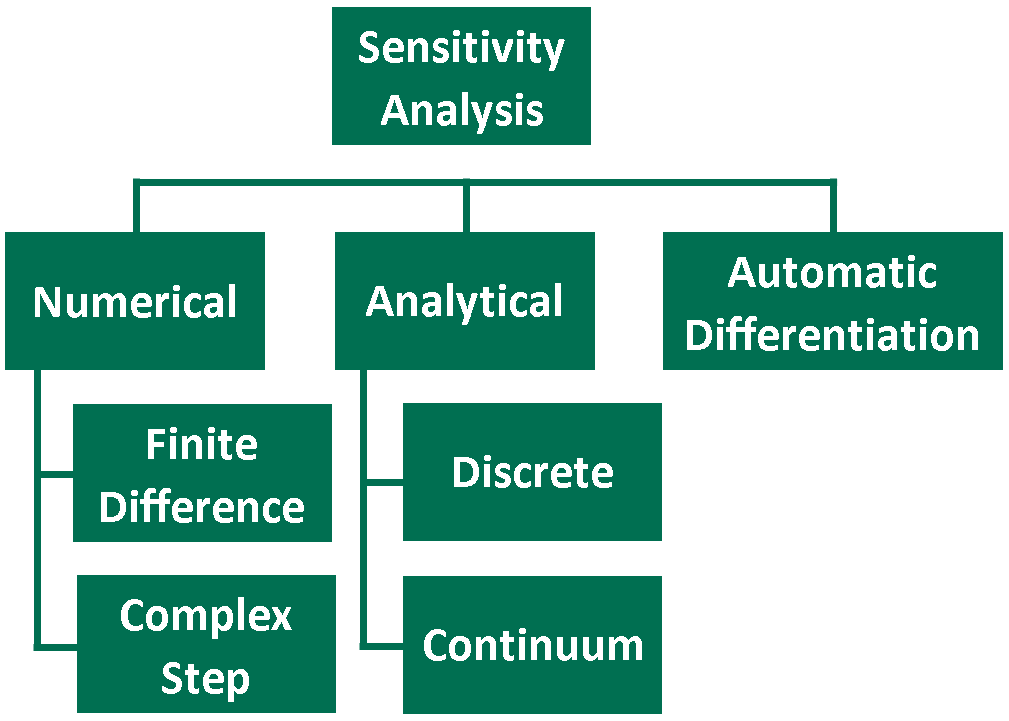
\includegraphics[height=7.00cm]{Chapter_1/figure/sensitivity_taxonomy.png}
	\caption{Sensitivity calculation techniques.}
	\label{fig:C1_sensitivityTaxonomy}
\end{figure}
%
The Finite Difference (FD) method is probably the easiest method to implement using a commercial software for calculating the sensitivity of a variable. The fact that they can be implemented even when a given computational model is treated as a black box makes most gradient-based optimzation algorithms perform finite differences by default when the user does not provide the required gradients. However, the computational cost associated with finite difference scheme for large systems can become very high. For a system with $n$ number of design variables, the analysis has to be performed $n+1$ times to calculate the design sensitivities. Furthermore, to ensure the accuracy, convergence study needs to be done for selecting the appropriate step size for the finite difference. The inaccuracy of finite differencing could result in convergence difficulties and inaccurate optimum results \cite{sobieszczanski1997multidisciplinary}.

Complex Step (CS) method avoids the loss of precision in finite differences approximation by employing complex arithmetic \cite{martins2003complex}. The complex step derivative is defined as shown in Equation \eqref{eq:C1_compelxStepFormula}.
%
\begin{equation}\label{eq:C1_compelxStepFormula}
	\mathcal{F}^\prime\left(u; b\right) = \frac{\text{Im}\left[ \mathcal{F}\left(u; b + ih\right) \right]}{h}
\end{equation}
%
where $\mathcal{F}\left(u; b\right)$ is the function of interest such as the airfoil lift that depends of a response variable, $u$ i.e. free-stream velocity, and design variable, $b$, i.e. shape of the airfoil. Complex step approximates the sensitivities by perturbing the design variable by an imaginary value of $ih$ and then evaluating the imaginary portion of the resulting response. Using the complex step method, we can choose a small step size for $h$ without loosing accuracy due to no subtraction involved in CS formulation. However, many commercial packages such as ANSYS or NASTRAN cannot handle complex arithmetic which makes the implementation of complex step method infeasible. Moreover, the high cost of finite difference is still associated with the complex method as well.

Automatic differentiation (AD) is based on the systematic application of the differentiation on computer programs \cite{naumann2012art}. In the AD approach, the chain rule of differentiation is applied to every line in the program assuming that the computer program consists of a sequence of explicit functions that act successively on some variables. Therefore, by differentiating each of these functions and applying the chain rule, it is possible to calculate the sensitivities. 

There has been extensive research on utilizing AD for optimization. Bischof et al. used AD for calculating the sensitivities using a CFD solver. They used ADIFOR for differentiating the source code of their CFD code (TLNS3D) which later was used for calculating the sensitivity of a transonic flow to change in the boundary conditions. Hascout et al., also used AD for a sonic boom reduction under a supersonic aircraft. In all of these works in order to implement AD, access is needed to the source code and modification of the solver extensively to calculate the sensitivities. This makes the use of this method for commercial codes impractical since the source code is usually not available.

The shortcomings of numerical and AD techniques demand more sophisticated methods for sensitivity calculation. These techniques are generally known as analytical methods. Formulation of the analytical sensitivities requires derivation of analytic sensitivity equations. These are obtained by differentiating the governing equations with respect to design variables such as shape of the boundaries. Analytical methods can be further categorized based on how the sensitivity equations are derived and solved. Typically, the continuum equations of the system are solved using an approximate method which discretizes the governing equations. The Discrete Sensitivity Analysis (DSA) technique differentiates the discretized governing equations with respect to design variables to acquire the analytical sensitivity equations \cite{choi2006structural}. The Continuum Sensitivity Analysis (CSA) differentiates the continuum equations for formulating the sensitivity equations. This system of equations is later discretized and solved for analytical sensitivities.

Regardless of continuum or discrete approach for deriving the sensitivity equations, these can be solved using two approaches: i) the direct method and ii) the adjoint method. This needs to be explained before talking about the sensitivity calculating techniques in detail. To better explain these two methods, let us use the finite element formulation for the displacement method of analysis.
%
\begin{equation}\label{eq:C1_finiteElementGE}
	KU = F
\end{equation}
%
where $K$ is the stiffness matrix that represents a structure, $U$ is the displacement vector, and $F$ is the load vector. The sensitivity of a response, $R$, (e.g. stress, displacement) with respect to a design variable, $b_i$, is determined by using chain rule for differentiation as shown in Equation \eqref{eq:C1_chainRuleGeneralResponse}.
%
\begin{equation}\label{eq:C1_chainRuleGeneralResponse}
	\frac{dR}{db_i} = \frac{\partial R}{\partial b_i} + 
	                  \frac{\partial R}{\partial U} \frac{\partial U}{\partial b_i}
\end{equation}
%
The best way to calculate the displacement sensitivity in Equation \eqref{eq:C1_chainRuleGeneralResponse} is to differentiate the governing Equation of \eqref{eq:C1_finiteElementGE} with respect to design variable $b_i$. 
%
\begin{equation*}
	\frac{\partial K}{\partial b_i} U + K \frac{\partial U}{\partial b_i} = \frac{\partial F}{\partial b_i}
\end{equation*}
%
The above equation is rewritten as
%
\begin{equation}\label{eq:C1_displacementSensitivity}
	\frac{\partial U}{\partial b_i} = 
	K^{-1} \underbrace{\left[ \frac{\partial F}{\partial b_i} - \frac{\partial K}{\partial b_i} U \right]}_\text{pseudo-loads}
\end{equation}
%
The response sensitivity, $dR/db_i$, is calculated by substituting Equation \eqref{eq:C1_displacementSensitivity} in \eqref{eq:C1_chainRuleGeneralResponse}. The \emph{direct} method first calculates the displacement sensitivity, $\dfrac{\partial U}{\partial b_i}$, and uses that to calculate $\dfrac{\partial R}{\partial U} \dfrac{\partial U}{\partial b_i}$ to form the response sensitivity. This method is performed once for each design variable. The \emph{adjoint} method first calculates $[K^{-1}]^T \left( \dfrac{\partial R}{\partial U}\right)^T$ and then takes dot product with the pseudo-load to form the second part of the response derivative. This method is performed once for each response. Therefore, if the number of responses are smaller than the design variables, the adjoint method will have better performance in terms of simulation cost \cite{vanderplaats1984numerical}.

The discrete sensitivity analysis has been historically the method of choice to calculate the high-accurate sensitivity when the details of analysis such as discretization approach and matrix assembly of discretized equations are available \cite{arora1979methods}. This method has been adopted by the structural optimization community and applied to fluid-solid interaction problems as well. Reuther et al., used the discrete method for aerodynamic shape optimization of a complex aircraft configuration \cite{reuther1999constrained}. They used Euler flow as the aerodynamics theory where they optimized different configurations for transonic and supersonic regimes only focusing on fluid pressure. Martins et al. developed an adjoint method for sensitivity analysis for an aero-structural aircraft design framework where the sensitivities were computed using a coupled adjoint approach. The framework was used on a supersonic business jet to calculate the sensitivity of drag with respect to the Outer Mold Line (OML) of the aircraft. They updated the shape of the wing airfoils by using Hicks-Henne functions. These airfoils were then linearly lofted to generate the wing. The advantage of Hicks-Henne functions is that when they are applied to a smooth airfoil, it remains smooth. In their work, the discretization details of the solver needed to be known to calculate the sensitivities since they used DSA \cite{martins2005coupled}. Newman et al. used this approach for aerodynamic shape sensitivity analysis and design optimization of geometrically complex configurations \cite{newman1997aerodynamic}. In their work, the flow is modelled using nonlinear Euler equations where the fluid domain is discretized using unstructured grid. They used highly efficient Gauss-Seidel and GMRES solvers for the solution of linear aerodynamics equations. The mesh deformation due to change in the optimization loop was performed by considering the mesh as a system of interconnected springs. They had to calculate the grid sensitivities by differentiating the grid adaptation algorithms which adds to the cost of the sensitivity analysis. Moreover, mesh deformation algorithms do not always result in usable domain for solving governing equations. For cases where the boundary deformation is large, mesh deformation fails due to tangled meshes or negative cell volumes \cite{morris2008cfd}. Jameson et al. also used unstructured grid for aerodynamic shape optimization \cite{cambridge2004aerodynamic}. They used adjoint formulation to calculate the aerodynamic shape sensitivities of a complete aircraft configuration. In their work, the flow is modelled using the Euler equation and the mesh deformation is performed using the spring method. Using DSA they were able to calculate the sensitivities of pressure coefficient of the aircraft wing with respect to its shape and use this data to optimize the shape of the wing. However, their method cannot be implemented in a commercial solver without access to the source code. Moreover, mesh deformation is still used in this approach which reduces the robustness of their technique. As a matter of fact, source code modification is essential in all other related research papers published in the area as well \cite{gamboa2009optimization, pandya1997gradient, kim2001aerodynamic, lyu2014aerodynamic}. However, the source code is usually inaccessible and very complex. Therefore, there is a great interest in sensitivity calculation techniques which require minimum knowledge of the analysis code. This can be achieved using the sensitivity formulation that operates on the governing equations before they are discretized. These methods are commonly known as Continuum Sensitivity Analysis (CSA) methods \cite{haftka1989recent}.

The CSA, involves solving a set of partial differential equations named the Continuum Sensitivity Equations (CSEs) to get the analytical sensitivities. When deriving the CSEs, the governing equations can either be differentiated in local or total form. The local formulation only reflects the effect of design variable of change on the response at a specific point in space. On the other hand, the total formulation of sensitivities takes the movement of physical points due to change in the shape of the domain into account.

Choosing between local and total differentiation depends on the Lagrangian or Eulerian representation of the governing equations. In the general case of continuum mechanics,  displacement and velocity are vectors. In any application, we have the choice of writing these vectors as functions of the position of material particles before deformation. This is called the Lagrangian description of motion and is really helpful for visualizing the deformations. This technique is mostly adopted in solid mechanics where we track the material points as the deformations are usually assumed to be small. However, in the fluid flow problems, since it is generally hard to identify a reference configuration and the deformations are large, it is preferable to write the displacement and velocities as functions of the deformed position of the particles. These quantities are now defined for a particular point in space that does not move with the particles. This is called the Eulerian description of motion.  As CSA was matured over the years, the computational fluids community adopted the local CSEs since its formulation is consistent with the Eulerian formulation of the governing equations \cite{borggaard1997pde, hristova2006continuous}. The structural optimization community adopted the total formulation for the sensitivities since its formulation was consistent with the Lagrangian formulation of structural mechanics. Nevertheless, the total and local formulations for the sensitivities can be converted from one form to the other. This will be explained in more detail in next chapter.

In summary, sensitivity analysis in general is more matured for structural problems than for fluid dynamics. Nevertheless, neither of these disciplines typically employ CSA for sensitivity calculation. The main reason for this is the need for higher derivatives on boundaries that can be hard to approximate \cite{cross2014local}. Aurora and Haug \cite{Arora}, followed by Dems and Mroz \cite{Dems-Mroz}, were among the first to develop the concept of CSA for structural optimization. They modeled the sensitivities as functionals allowing them to convert the sensitivity integrals over the entire domain to the integrals over the boundaries. Although using this approach is possible to reduce the cost of the simulation, accurate values of functionals are required at the boundaries. This is not always achievable, especially for finite element analysis where the solution accuracy drops near the boundaries. The lack of applicability of CSA in structural optimization is due to the complicated definition of the boundary conditions and maturity of discrete methods for the sensitivity calculation. In recent years, Cross and Canfield \cite{cross2014local} developed specific local CSA formulation to handle these issues. They used Spatial Gradient Reconstruction (SGR) technique to approximate the gradient with higher-order accuracy near the boundaries. This is essential for calculating accurate sensitivities.

The first application of CSA in optimization problems for fluid dynamics is the work by Jameson \cite{jameson1988aerodynamic} on adjoint formulation for aerodynamic shape optimization. Borggaard and Burns \cite{borggaard1995sensitivity} implemented a direct formulation for shape sensitivity analysis of inviscid supersonic flows over rigid bodies. Stanley and Stewart \cite{stanley2002design} applied CSA in a fluid mechanics discipline with a goal for aerodynamic design. Pelletier and Etienne have applied CSA to numerous fluid-structure interaction (FSI) problems \cite{etienne2005general} focused mainly on sensitivities of fluid flow parameters near the structure. Liu and Canfield have employed CSA for shape optimization of nonlinear structures subject to an aeroelastic gust response \cite{liu2013equivalence}. They used the finite element method to solve the potential flow around an airfoil and applied CSA to find the airfoil pressure coefficient sensitivity with respect to the maximum camber. 

In almost all of the research done on sensitivity calculation of flow field to shape design variable, body conformal grids were used. The conforming mesh methods consider the interface conditions as physical boundary conditions, which treat the interface location as part of the solution and requires meshes that conform to the interface. Using this approach it is possible to represent the solid boundary shape with good accuracy. However, due to the coupling of fluid mesh topology and solid boundary shape, with the movement and/or deformation of the solid structure, re-meshing (or mesh-updating) is needed. This is a major problem when dealing with coupled fluid-structure analysis or shape optimization of any kind. Although conforming mesh methods have been widely used in many FSI problems, they are cumbersome, if not impossible, to apply to problems with large deformations \cite{sahin2009arbitrary}. The other shortcoming of body-conformal grids is the effect of mesh deformation on the sensitivity analysis. Since the computational domain is affected by change in the shape of the boundaries, it is required to calculate the mesh sensitivities \cite{liu2013boundary} for discrete sensitivity analysis. This adds to the computational effort for calculating  sensitivities.

The shortcoming of a robust grid generation and the additional cost of calculating mesh sensitivities motivated an important research effort to develop a technique that does not require fluid domain's mesh modification throughout the optimization iterations. One of the possible candidates to achieve this goal is the use of Immersed Boundary (IB) methods to decouple the fluid mesh from the shape of solid domain.
% ---------------------------------------------------------------------------------------------
\subsection{Immersed Boundary Method}
Traditionally the analysis techniques for flow over complex bodies are based on body-fitted multi-block or unstructured grid methods. However, in the last decade another class of techniques, called the immersed boundary methods, has been introduced. The term immersed boundary was first used by Peskin \cite{peskin1977numerical} to simulate the blood flow through heart valves. What distinguishes this method from the other methods for representing the solid boundaries is that the flow is solved on the Cartesian grid that does not necessarily conform to the boundaries. Therefore, the mesh generation is greatly simplified and in case of moving/deforming boundaries, there is no need to update the mesh during simulation. A separate formulation is used to impose the effect of the boundaries on the governing equations.

Consider the simulation of flow past a circular cylinder as shown in Figure \ref{fig:C1_conformalVSnonconformal}. Generating structured or unstructured grids is achieved in two steps. First, a surface grid covering the boundaries is generated. This is then used as a boundary condition to generate a grid in the volume occupied by the fluid. The differential form of the governing equations is then transformed to a curvilinear coordinate system aligned with the grid lines \cite{anderson1995computational}. The governing equations are then discretized on this curvilinear grid and solved using appropriate technique.
%
\begin{figure}[H]
	\centering
	\subfigure[Conforming mesh, $t = t_1$]
	{
	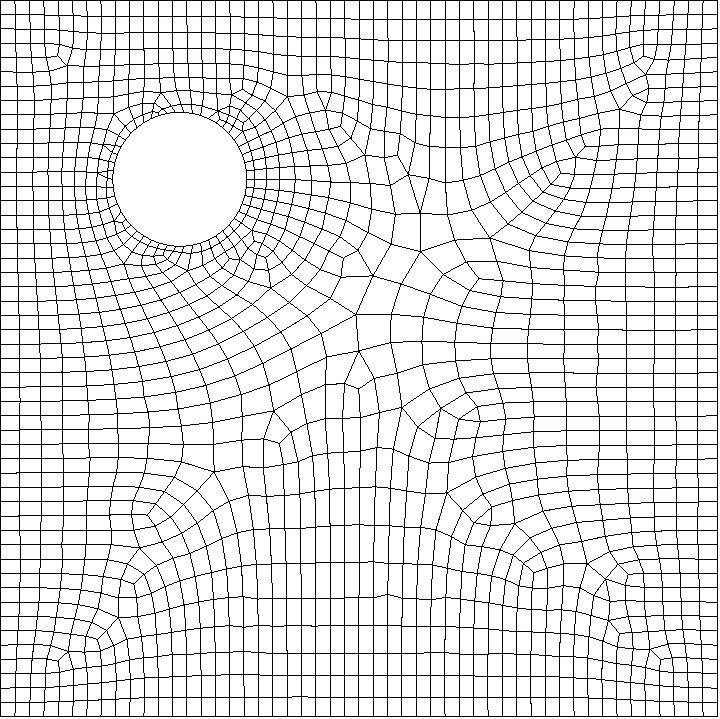
\includegraphics[height=5.0cm]{Chapter_1/figure/conforming_t1.jpg}
	}
	\quad
	\subfigure[Conforming mesh, $t = t_2$]
	{
	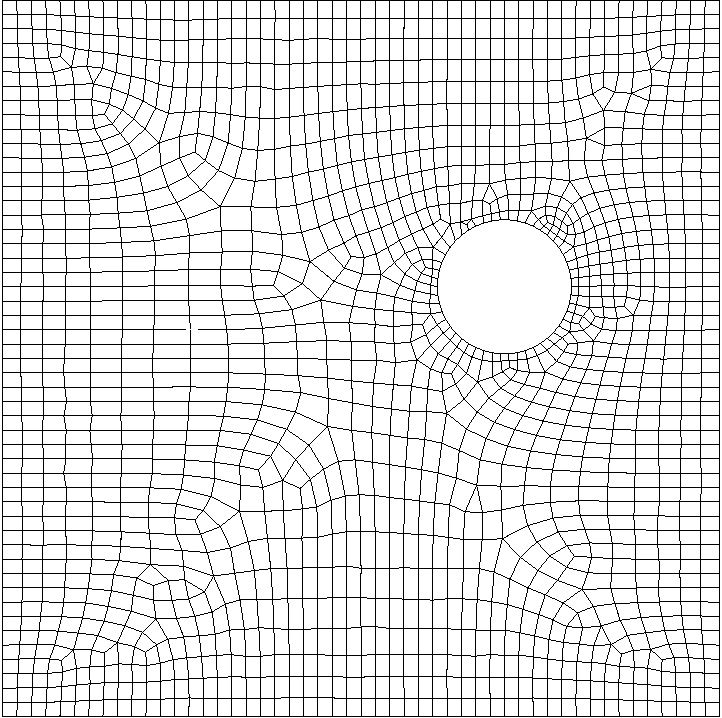
\includegraphics[height=5.0cm]{Chapter_1/figure/conforming_t2.jpg}
	}
	\\
	\subfigure[Nonconforming mesh, $t = t_1$]
	{
	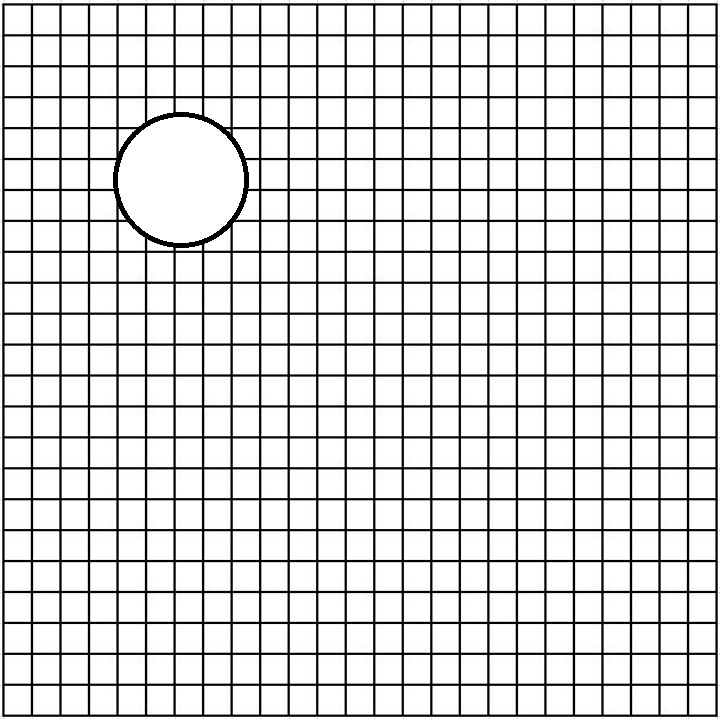
\includegraphics[height=5.0cm]{Chapter_1/figure/nonconforming_t1.jpg}
	}
	\quad
	\subfigure[Nonconforming mesh, $t = t_2$]
	{
	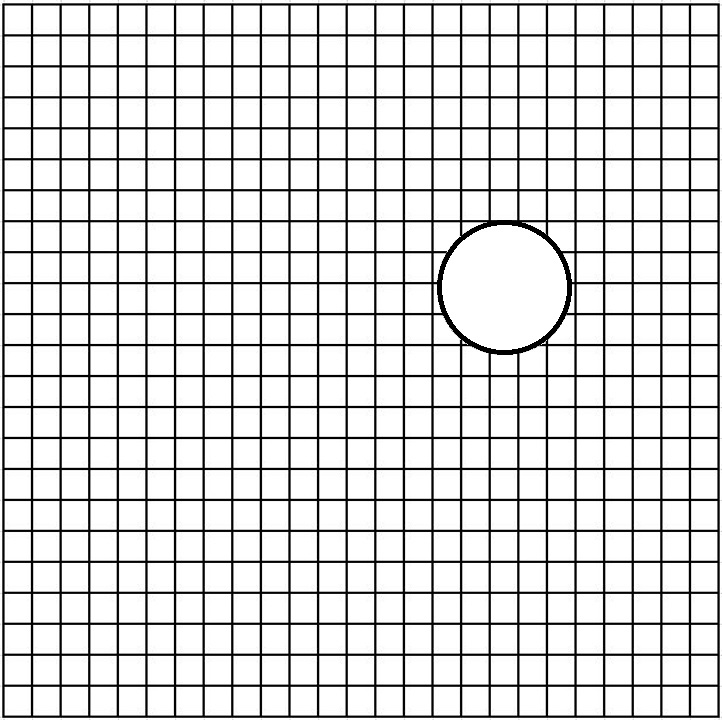
\includegraphics[height=5.0cm]{Chapter_1/figure/nonconforming_t2.jpg}
	}
	\caption{Example of conforming and nonconforming meshes.}
	\label{fig:C1_conformalVSnonconformal}
\end{figure}
%
Non-body-conformal Cartesian grid can also be utilized for this simulation as shown in Figure \ref{fig:C1_conformalVSnonconformal}. In this approach, the IB would still be represented through some means such as a surface grid, but the Cartesian volume grid would be generated with no regard to this surface grid. Thus, the solid boundary would cut through this Cartesian volume grid. Because the grid does not conform to the solid boundary, incorporating the boundary conditions would require modifying the equations in the vicinity of the boundary. Assuming that such a procedure is available, the governing equations would then be discretized using a finite-difference, finite-volume, or finite-element technique without resorting to coordinate transformation or complex discretization operators.

Depending on how the effect of solid boundaries are imposed, IB methods can be divided into three categories: i) Continuous forcing, ii) discrete forcing, and iii) cut-cell method.

The continuous forcing method was originally used by Peskin \cite{peskin1977numerical} and later further developed by other researchers \cite{saiki1996numerical, zhu2003interaction, beyer1992analysis}. In this approach, the boundary configuration is described by a curve $x(s,t)$ (Lagrangian nodes) where the location of each point on this boundary is governed by its equations of motion. The forces that the curve $x(s,t)$ exerts on the fluid is calculated by the constitutive law of the curve $x(s,t)$ that relates the displacements to stress values. These stress values are transferred to the Navier-Stokes (NS) (Eulerian nodes) for the fluid by means of a Dirac delta function. Practical implimentation of this method rests in representing the Dirac delta function as a discrete function that has the same properties. This method is applied to a variety of problems, including Cardiac blood flow \cite{peskin1989three}, animal locomotion \cite{fauci1988computational}, multiphase flows \cite{kempe2015imposing}, and particle sedimentation \cite{uhlmann2005immersed}.

Peskin's method is well suited for elastic boundaries. For stiff boundaries, the constitutive laws of the solid boundaries will result in instabilities in the solution of governing equations \cite{mittal2005immersed}. The virtual boundary method of Goldstein \cite{goldstein1993modeling} enables us to handle these rigid boundaries. The main idea of this approach is the same as Peskin's method where the solid boundary is treated as a virtually existing surface embedded in the fluid. The force on this surface is calculated by the requirement that the fluid velocity should satisfy the no-slip condition. Since this body force is not known a priori, it is calculated in a feedback way.

The penalization method is also categorized under the continuous forcing approaches to the IB problem. This technique is based on the Brinkman equation that describes the fluid flow through a porous medium. The Brinkman equation is analogous to Fourier's laws in heat conduction and Ohm's law in the field of electrical engineering \cite{durlofsky1987analysis}. This approach was first proposed by Arquis and Caltagirone \cite{arquis1984conditions} where they imposed the boundary conditions by adding the penalization terms to the momentum equations. The main idea of this approach is to model the solid obstacles as a porous medium with porosity of $\mathcal{K}$. Porosity is a measure of void spaces in a material. Therefore, by selecting low values for porosity, the porous domain acts as a solid wall. It has been demonstrated that the solution of the penalized incompressible NS equations converge to the exact solution as the porosity approaches zero \cite{angot1999analysis}; however, in the practical implementation, extremely low values for porosity will result in systems with a very large stiffness that are numerical instability. To apply the porosity within the solid domain, a Heaviside function is used by other researchers \cite{gazzola2011simulations, kevlahan2001computation}.

The continuous forcing approach is very attractive for flows for both rigid and elastic boundaries due to its ease of implementation. This technique can be added to an already available commercial package such as ANSYS Fluent for CFX with limited effort. One of the shortcomings of this approach is the smoothing of the forcing function near the boundary. This can result in inability for sharp representation of the immersed boundary in cases such as compressible flows. However, accuracy for representing the boundaries can be improved by refining the mesh and using higher-order force mapping schemes.

Mohd-Yusof formulated the discrete formulation of IB method \cite{mohd1997combined} for addressing the time penalties associated with the simulation involving moving boundaries. The main idea of this technique is same as the virtual boundary method where a force term is added to momentum equations to represent the solid boundary. However, the momentum equation manipulation is done in the discrete manner. In the work of Mohd-Yusof \cite{mohd1997combined} and Verzicco et al. \cite{verzicco1998complex} this is done by modifying the discretization stencil in the vicinity of the boundary curve so that the velocity values on this boundary satisfy a pre-defined condition. The major advantage of this approach is the absence of user specified parameters; however, its implementation depends strongly on the discretization approach used for the analysis. Therefore, it cannot be easily implemented nonintrusively with commercial codes. This implementation of discrete forcing method has been applied to many different problems such as turbulent flow inside an internal combustion engine \cite{verzicco1998complex}, flow past 3D bluff bodies \cite{verzicco2002large}, and flow in a cylindrical stirred tank \cite{iaccarino2003immersed}.

In the cut-cell methods, the grid cells are cut by the solid boundary and reshaped so that they form a boundary-conforming, unstructured grid. This is shown in Figure \ref{fig:C1_cutCellMesh}.

\begin{figure}[H]
	\centering
	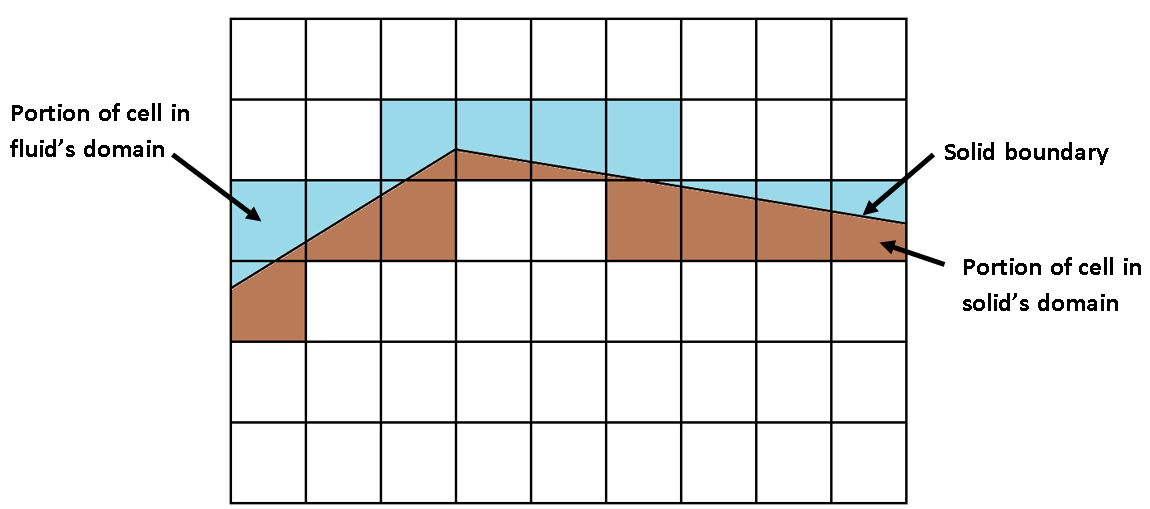
\includegraphics[height=7.0cm]{Chapter_1/figure/cut_cell_mesh}
	\caption{Modified mesh near the solid boundary for cut-cell method.}
	\label{fig:C1_cutCellMesh}
\end{figure}

The cut-cell method was first introduced by Clarke \cite{clarke1986euler} for inviscid flows. This method has been applied to both collocated and staggered grids \cite{kirkpatrick2003representation} however, most applications were focused on 2D flows \cite{hu2006conservative, udaykumar1999computation}. This is because of the many possibilities for the geometrical shape of the cut-cell, that makes the flux calculation and therefore numerical implementation extremely difficult.

% ---------------------------------------------------------------------------------------------
\subsection{Sensitivity Analysis for IB Method}
The body of the research done in the immersed boundary community has been concentrated on the improvement of method accuracy and resolving the stability issues. However, there has not been much effort in the sensitivity calculation using an IB formulation. There has been some research on the sensitivity analysis using the penalization framework. Borrvall and Petersson applied the penalization method for topology optimization of fluids in Stokes flow \cite{borrvall2003topology}. They used the discrete sensitivity analysis to calculate the sensitivity of fluid pressure to the shape of the boundaries. They used this technique to optimize the shape of a diffuser and a pipe bend. They verified their methodology for outflow problems as well, where they optimized the shape of solid domain to maintain the least possible pressure drop by constraining the penalized region volume.  Challis and Guest investigated the level set formulation for the topology optimization of fluids in Stokes flow \cite{challis2009level}. They used the penalization technique to formulate the no-slip condition on the solid boundaries. They implemented the topological sensitivities in their solver where they used power dissipation minimization to optimize the shape of a diffuser and a connecting 3D pipe. The penalization method is probably the easiest of the IB methods to implement. This is because it does not have a free parameter such as in virtual boundary method and does not depend on the discretization such as discrete forcing methods. Moreover, no interpolation is needed for applying penalization method to a computational domain. In the penalization method, the fluid and solid domains are differentiated based on a scalar function (porosity) which is very similar to the density-based approaches in the topology optimization community \cite{deaton2014survey}. This is probably the biggest reason for researchers to use penalization technique for shape optimization using IB method, since the available techniques from topology optimization community can be used \cite{leveque1997immersed, pingen2007topology}. Similar to topology optimization, the shortcoming of penalization technique is in its accuracy for representing the boundaries. Since the nodes are assigned with the porosity values, it is extremly difficult if not impossible to control the exact location of the immersed boundary if it does not coincide with the computational nodes. Moreover, the current demonstration problems for the penalization technique are only applicable to low Reynolds numbers flow.

% ---------------------------------------------------------------------------------------------
\section{Research Contribution}
Design optimization for coupled fluid-solid interaction problems is a challenging effort. The current state-of-art technique handles the MDO problem by using unstructured grid and using DSA for sensitivity calculation. However, these techniques cannot be used along with an arbitrary software packages without a deep understanding of how the governing equations are formulated and discretized within the solver. Moreover, due to the use of body-conformal grids for fluid domain discretization, additional cost and effort are introduced in both the analysis and sensitivity calculation. Approximating the mesh sensitivities and mesh deformation are two examples for this extra calculation. This research presents a specific formulation for immersed boundary method along the continuum sensitivity analysis for satisfying both of the issues regarding mesh deformation and sensitivity implementation \cite{gobal2014continuum}. The specific contributions of this research are as follows:

\begin{itemize}
	\item Two different classes of continuous immersed boundary methods are explained and used within CSA framework to calculate the sensitivity of different flow parameters with respect to shape design variables. The immersed boundary method is based on relaxed Dirac delta functions to transfer the data between the fluid and structure domains; however, this formulation cannot be used within the CSA framwork. Smooth representation for Dirac delta function is developed for this purpose.
	\item This research is the first application of CSA for sensitivity analysis of fully coupled FSI simulation modeled with IB technique. IB method enables us to have a robust FSI simulation and also have the high-fidelity solution of the NS equations. The sensitivity analysis builds on top of this framework so it can be used for shape design optimization of such problems using gradient-based optimization techniques.
	\item The use of continuum immersed boundary methods for sensitivity analysis of flows with moderate to high Reynolds numbers is another contribution of this work. Most of the previous works done in this area regarding the sensitivity analysis are based on flows with lower Reynolds numbers such as Stokes flows.
\end{itemize}

\chapter{Design Sensitivity Analysis}
In this chapter, the concept behind discrete and continuum sensitivity formulation is discussed and the general approach for deriving the sensitivity equations is presented. The difference between local and total formulation of the sensitivity response is discussed and finally the independence of continuum sensitivity formulations to discretization method is proven. This enables us to reuse the solver of governing equations to calculate the sensitivity response. This is typically not possible for discrete sensitivity formulation. The two sensitivity analysis techniques are applied to a heat transfer benchmark problem where the sensitivity of response to the shape of the domain is calculated. This problem is also used in the next chapter for implementation of different immersed boundary methods.

% ======================================================================================
\section{General Formulation}
The general shape for the computational domain is defined in Figure \ref{fig:C2_continuumDomain}. The response variable on this domain can represent a fluid, i.e. pressure or velocity, or can be calculated for a solid, i.e. displacements. Nevertheless, in any of these cases the response is calculated by solving a governing equation subject to boundary conditions. 

\begin{figure}
	\centering
	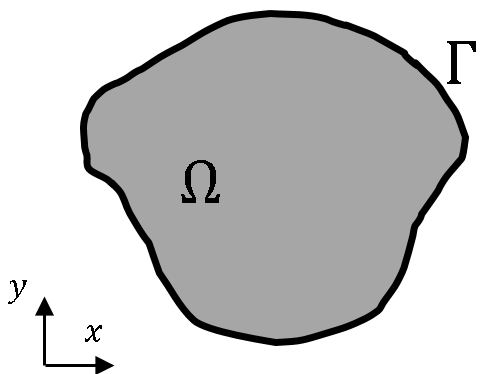
\includegraphics[width=4.00cm]{Chapter_2/figure/general_domain.png}
	\caption{General computational domain $\Omega$ with boundary $\Gamma$.}
	\label{fig:C2_continuumDomain}
\end{figure}

In this work, the governing equation and the boundary conditions are represented in the functional form as shown in Equation \eqref{eq:C2_governingEquationAndBC}.

\begin{subequations}\label{eq:C2_governingEquationAndBC}
\begin{equation}\label{eq:C2_generalGoverningEquation}
	\mathbf{A}(\mathbf{u}, t; \mathbf{b}) = \mathbf{f}(\mathbf{x}, t; \mathbf{b})
	\quad \text{on} \quad \Omega
\end{equation}
\begin{equation}\label{eq:C2_generalBoundaryCondition}
	\mathbf{B}(\mathbf{u}, t; \mathbf{b}) = \mathbf{g}(\mathbf{x}, t; \mathbf{b})	
	\quad \text{on} \quad \Gamma
\end{equation}
\end{subequations}

where $\mathbf{A}$ is the governing equation such as Navier-Stokes equations for the fluid or elastic equations for the solid domain and $\mathbf{B}$ is the boundary condition. $\mathbf{u}$ is the response variable such as displacement or pressure. $t$ is time, $\mathbf{b}$ is the design variable such as shape or size, and $\mathbf{x}$ is the spatial coordinate. $\mathbf{f}$ and $\mathbf{g}$ are the values of governing equation and boundary conditions. It should be noted that in this formulation, the functions $\mathbf{A}$ and $\mathbf{B}$ are only implicitly dependent on the design variable $\mathbf{b}$. This is important when deriving the sensitivity equations later in this chapter. This implicit dependence is represented by using the semicolon symbol in the definition of $\mathbf{A}$ and $\mathbf{B}$.

For the general case of problem formulation, the total sensitivity of response variable, $\mathbf{u}$, with respect to the $i$-th design variable, $b_i$, is written as

\begin{equation}\label{eq:C2_totalSensitivityDef}
	\frac{D \mathbf{u}}{D b_i} = 
	\underbrace{\frac{\partial \mathbf{u}}{\partial b_i}}_\text{local derivative} + 
	\underbrace{\frac{\partial \mathbf{u}}{\partial \mathbf{x}} \cdot
	\frac{\partial \mathbf{x}}{\partial b_i}}_\text{convective term}
\end{equation}

The total derivative is known as material derivative in continuum mechanics \cite{mase2009continuum}. This total sensitivity defines the change of response variable, $\mathbf{u}$, with respect to design variable and space dependent changes. The material derivative consists of the local derivative, $\partial \mathbf{u}/\partial b_i$, plus the convective term, $\partial \mathbf{u}/\partial \mathbf{x} \cdot \partial \mathbf{x}/\partial b_i$. The local derivative is the measure of change in the response variable due to change in the design parameter. Whereas, the convective term accounts for the movement of points in space due to change in the design variable. This is specially applicable to shape sensitivity analysis where the change in design variable, will clearly cause the material points to move \cite{cross2014local}.

The convective term consists of two separate gradients: i) $\partial \mathbf{u} / \partial \mathbf{x}$ which represents the spatial gradient of the response variable, and ii) $\partial \mathbf{x} / \partial b_i$ that defines the sensitivity of the location of computational nodes with respect to changes in the design variable. The response gradient, $\partial u/\partial x$, is calculated from the analysis results, using finite difference approach or derivative of shape functions in FEA formulation. Calculation of domain sensitivity, $\partial \mathbf{x} / \partial b_i$, requires more attention.

A common approach for calculating the domain sensitivity, is to use the techniques used to deform the body-conformal mesh in CFD/FEA simulations. These methods are usually based on representing the computational grid as a system of springs that connected to each other at the nodes. This system is modeled and solved using structural analysis techniques, where the sensitivities can be easily implemented. This is effectively a shape sensitivity analysis for the structural problem \cite{haftka1986structural}. This step is removed from the analysis if the computational domain is not affected by the design variable since $\partial x/\partial b$ is equal to zero \cite{gobal2014continuum}. This is one of the reasons to use the immersed boundary calculation since it reduces the cost of the simulation. This is discussed in more details in Chapter \ref{ch:immersedBoundary}.

% ======================================================================================
\section{Benchmark Cases}
To compare the discrete and continuum sensitivity analysis formulations, two problems from different disciplines are selected. As a simplified representation for the fluid/thermal systems, the one-dimensional heat transfer analysis in a beam is selected. This problem is used by different researchers for investigating sensitivity analysis for nonlinear systems \cite{dowding2001sensitivity} and thermal design and monitoring \cite{szopa2005second, sorli2004computational}. The special interest in this problem is due to availability of analytical solution since this can be used to verify the numerical results of the sensitivity analysis.

To compare the discrete and continuum sensitivity analysis formulations, the one-dimensional heat transfer analysis in a beam is chosen. The temperature is governed by the Laplace equation as shown in Equation \eqref{eq:C2_laplaceEquation}.

\begin{equation}\label{eq:C2_transientHeatEquation}
	\frac{\partial^2 T}{\partial x^2} = \frac{1}{\alpha} \frac{\partial T}{\partial t}
\end{equation}

where $T$ is the temperature, $x$ is spatial variable, $t$ is time, and $\alpha$ is the thermal diffusivity. For this problem we are only interested in the steady state solution of the system, therefore the right-hand-side of Equation \eqref{eq:C2_transientHeatEquation} is equal to zero. Therefore, the governing equation for this problem is written as

\begin{equation}\label{eq:C2_laplaceEquation}
	\frac{\partial^2 T}{\partial x^2} = 0
\end{equation}

The boundary conditions are defined as constant temperatures at the two ends of the domain as $T_0$ and $T_L$. The length of domain is selected as $L$. This is shown in Figure \ref{fig:C2_benchmarkCase}

\begin{figure}[h]
	\centering
	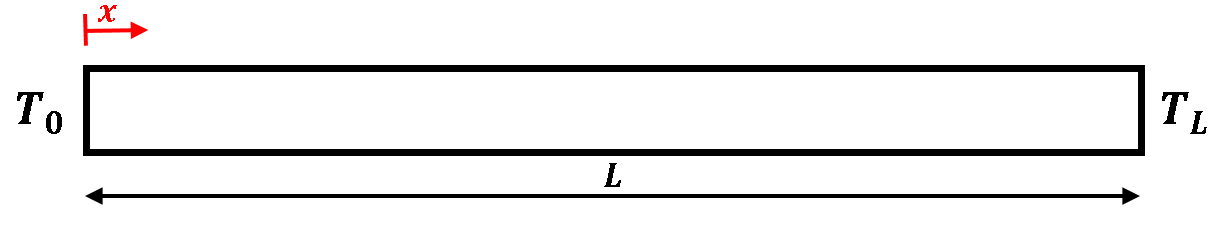
\includegraphics[width=14.00cm]{Chapter_2/figure/benchmark_case.png}
	\caption{One dimensional domain with heat conduction.}
	\label{fig:C2_benchmarkCase}
\end{figure}

The analytical solution for this problem is available and is written as shown in Equation \eqref{eq:C2_benchmarkCaseAnalyticalSolution}

\begin{equation}\label{eq:C2_benchmarkCaseAnalyticalSolution}
	T = \frac{T_L - T_0}{L} x + T_0
\end{equation}

The analytical sensitivity of the temperature with respect to beam's length is calculated by differentiating Equation \eqref{eq:C2_benchmarkCaseAnalyticalSolution} with respect to $L$.

\begin{equation}
	\frac{\partial T}{\partial L} = -\frac{T_L - T_0}{L^2} x
\end{equation}

This is later used for verifying the discrete and continuous sensitivity results.

% ======================================================================================
\section{Discrete Sensitivity Formulation}
The discrete sensitivity equations are formulated by discretizing the governing equation \eqref{eq:C2_laplaceEquation} using finite difference method. It should be noted that the finite difference is used for discretization of continuum governing equation and not for sensitivity calculation. Other techniques such as finite volume or finite elements can be used for the discretization of the governing equations as well. For this problem, the design variable affects the shape of the domain which is related to the distance between the nodes in the discrete manner. Therefore, for the sake of sensitivity analysis it is required to keep the nodal distances in the discretized solution as well. The domain is discretized by using 6 nodes as shown in Figure \ref{fig:C2_discretizedDomain}.

\begin{figure}[h]
	\centering
	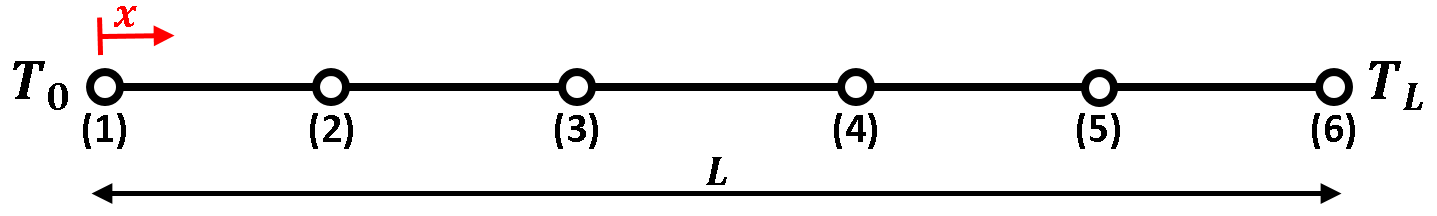
\includegraphics[width=14.00cm]{Chapter_2/figure/benchmark_case_computational_domain.png}
	\caption{One dimensional computational domain for the heat conduction problem.}
	\label{fig:C2_discretizedDomain}
\end{figure}

The second derivative of Equation \eqref{eq:C2_laplaceEquation} needs to be approximated for discretization. This is done by writing the Taylor series expansion of temperature at arbitrary location $x_i$. By using the central difference method the second order approximation for the second order derivative is written as shown in Equation \eqref{eq:C2_finiteDifferenceSchemes}.

To maintain the generality, we assume that distance of node $T_i$ to $T_{i+1}$ is $\Delta_i$ and the distance of node $T_i$ to $T_{i-1}$ is $\Delta_{i-1}$.

\begin{equation}\label{eq:C2_finiteDifferenceSchemes}
	\frac{\partial^2 T}{\partial x^2} = 
	\frac{T_{i-1} \Delta_{iL} - 
	      T_{i} (\Delta_{iL} + \Delta_{iR}) + 
	      T_{i+1} \Delta_{iR}}
	     {\dfrac{1}{2} \left[ \Delta_{iL} \Delta_{iR}^2 + 
	                         \Delta_{iL}^2 \Delta_{iR} \right]}
\end{equation}

The discretized governing equation of \eqref{eq:C2_finiteDifferenceSchemes} is written in a matrix form as shown in Equation \eqref{eq:C2_laplaceEquationMatrixForm}.

\begin{equation}\label{eq:C2_laplaceEquationMatrixForm}
	\begin{bmatrix}
		\frac{-2}{\Delta_{1} \Delta_{2}} &
		\frac{2}{\Delta_{1} \Delta_{2} + \Delta_{1}^2} &
		0 &
		0 &
		\\
		\frac{2}{\Delta_{3}^2 + \Delta_{2} \Delta_{3}} & 
		\frac{-2}{\Delta_{2} \Delta_{3}} &
		\frac{2}{\Delta_{2} \Delta_{3} + \Delta_{2}^2} &
		0
		\\
		0 &
		\frac{2}{\Delta_{4}^2 + \Delta_{3} \Delta_{4}} & 
		\frac{-2}{\Delta_{3} \Delta_{4}} &
		\frac{2}{\Delta_{3} \Delta_{4} + \Delta_{3}^2} &
		\\
		0 &
		0 &
		\frac{2}{\Delta_{5}^2 + \Delta_{4} \Delta_{5}} & 
		\frac{-2}{\Delta_{4} \Delta_{5}}
	\end{bmatrix}
	\begin{bmatrix}
		T_2 \\
		T_3 \\
		T_4 \\
		T_5
	\end{bmatrix}
	=
	-\begin{bmatrix}
	 	\frac{2T_1}{\Delta_{2}^2 + \Delta_{1} \Delta_{2}} \\
 		0 \\
		0 \\
		\frac{2T_6}{\Delta_{5} \Delta_{4} + \Delta_{5}^2}
	\end{bmatrix}
\end{equation}

To verify the discretization process, we compare the analytical solution of this problem with the result of Equation \eqref{eq:C2_laplaceEquationMatrixForm} in Figure \ref{fig:C2_verificationOfSolver}. For this problem we choose $T_1 = 0$, $T_6 = 1$ as the boundary conditions, and $L = 1$.  As shown in this figure, the discrete and continuum results match very well for different number of nodes. This is done by comparing the absolute error between the analytical and approximate results as shown in Table \ref{table:C2_solutionError}.

\begin{figure}[H]
	\centering
	\subfigure[$n = 6$]
	{
	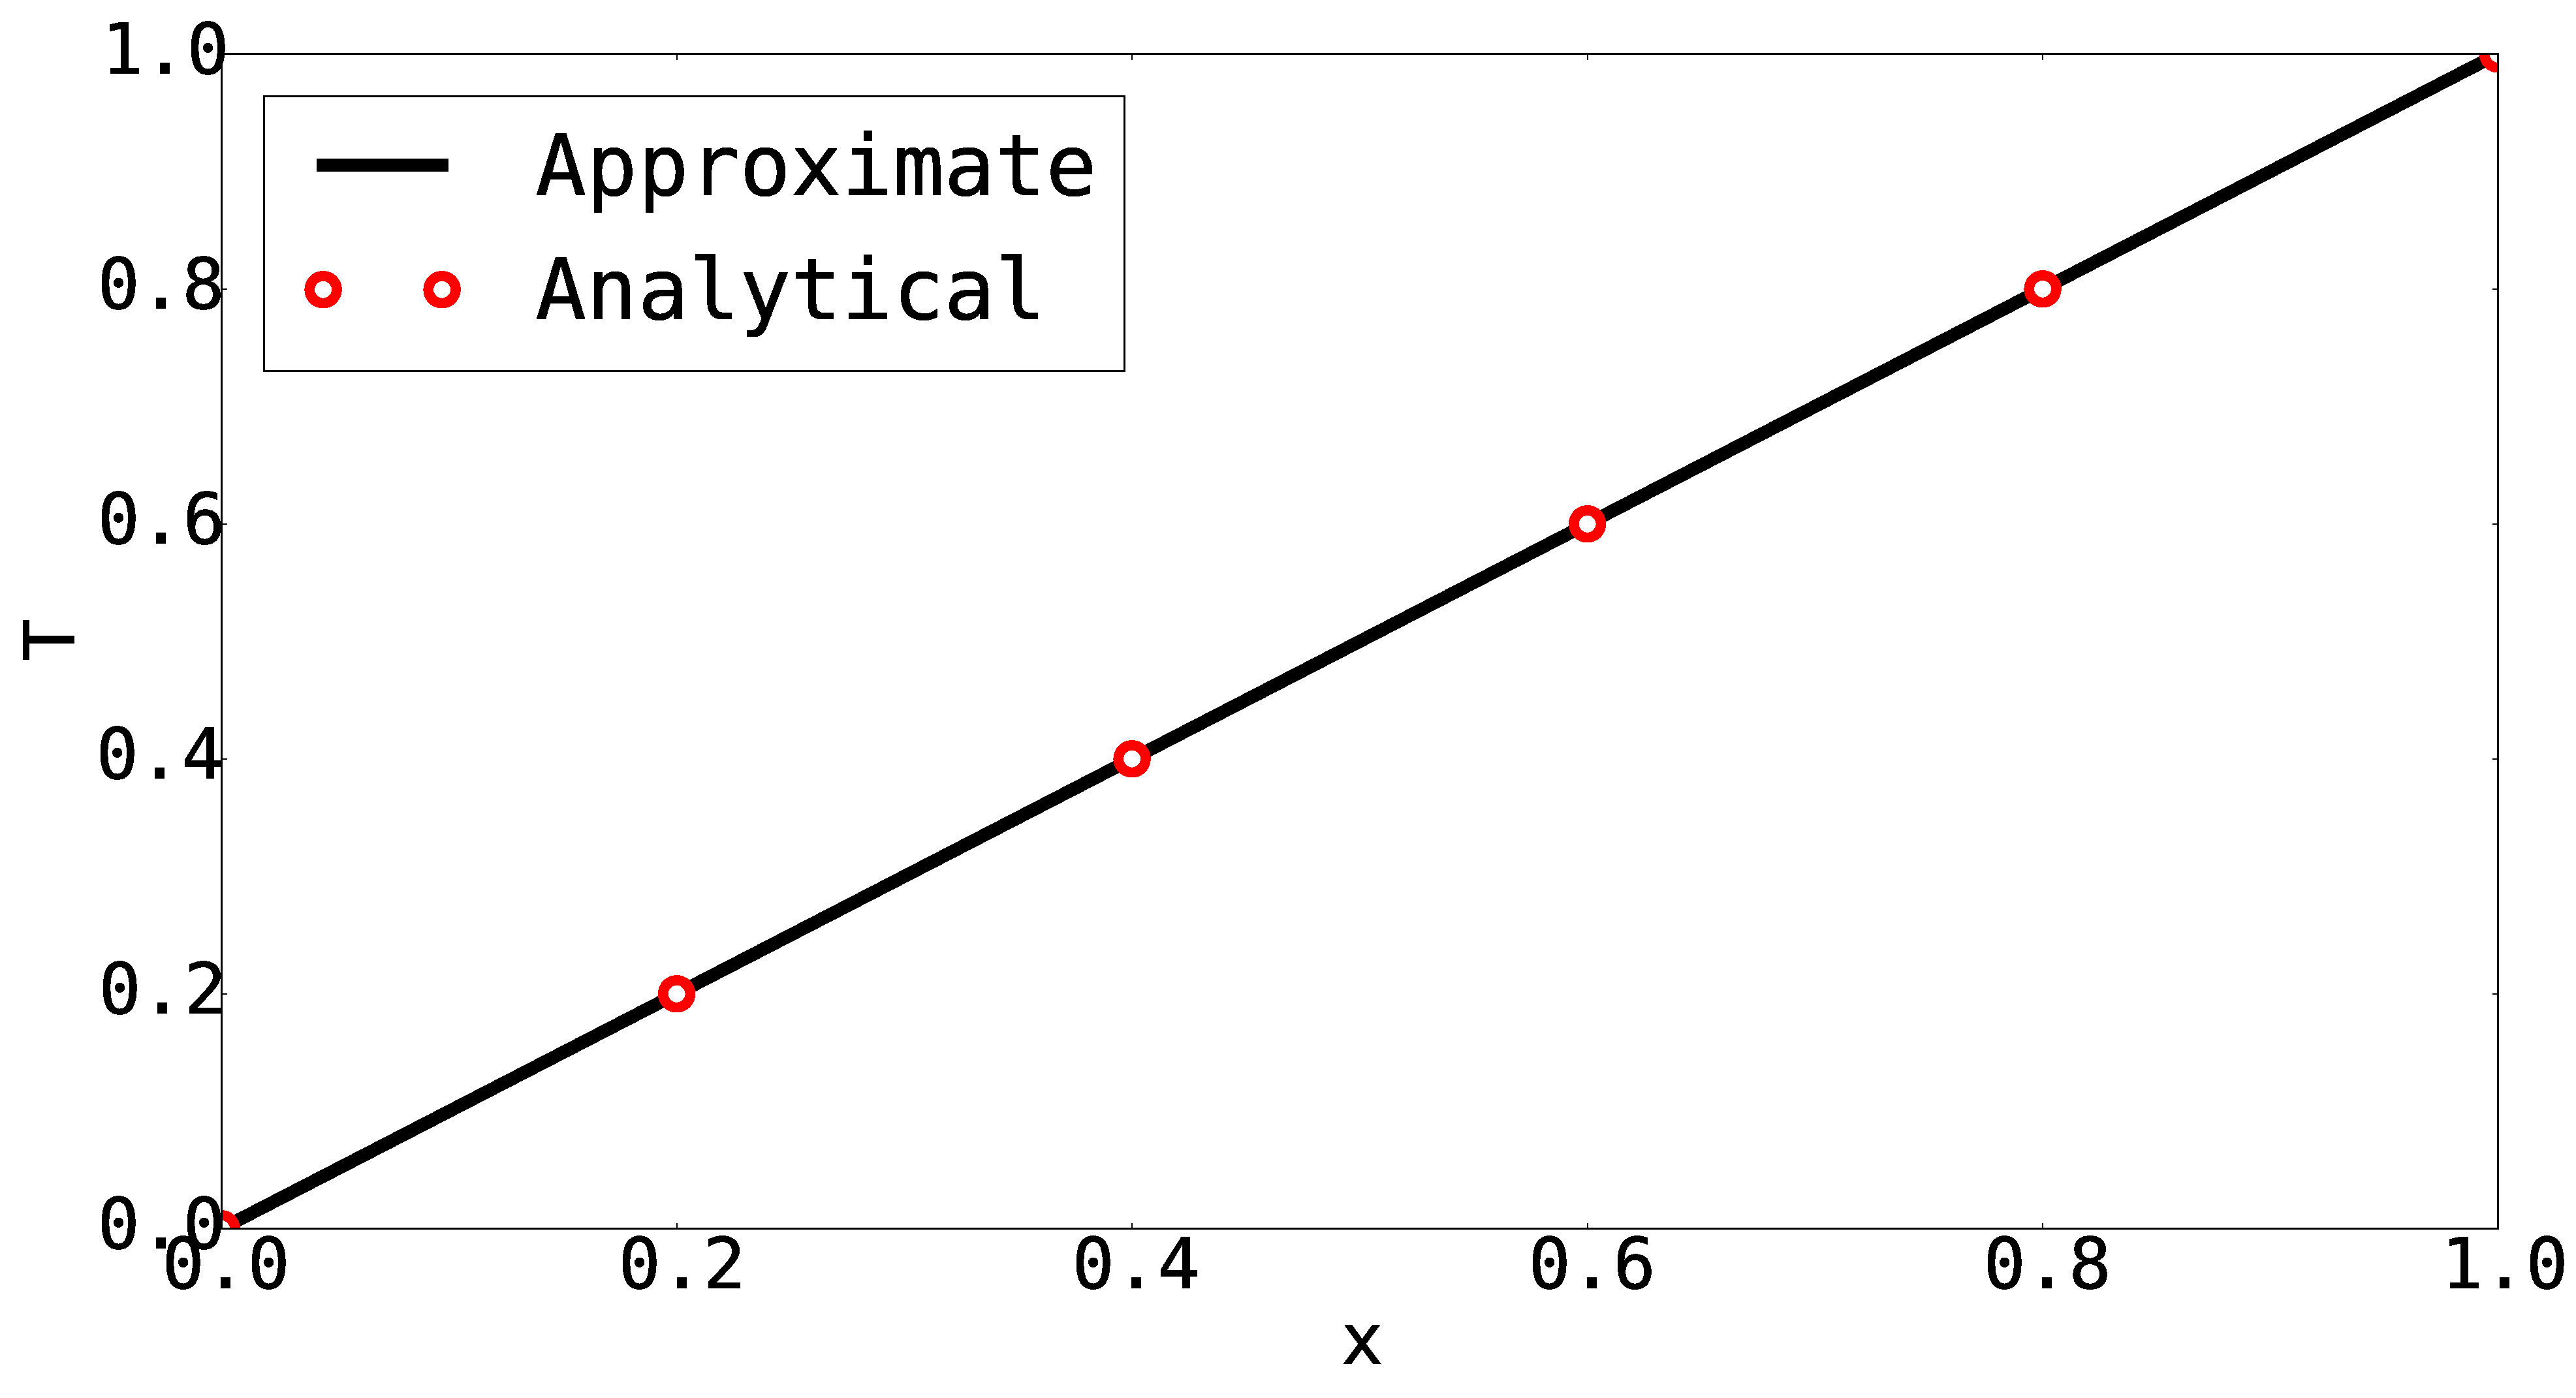
\includegraphics[width=7.0cm]{Chapter_2/figure/finitedifference_vs_analytical_n6.eps}
	}
	\quad
	\subfigure[$n = 12$]
	{
	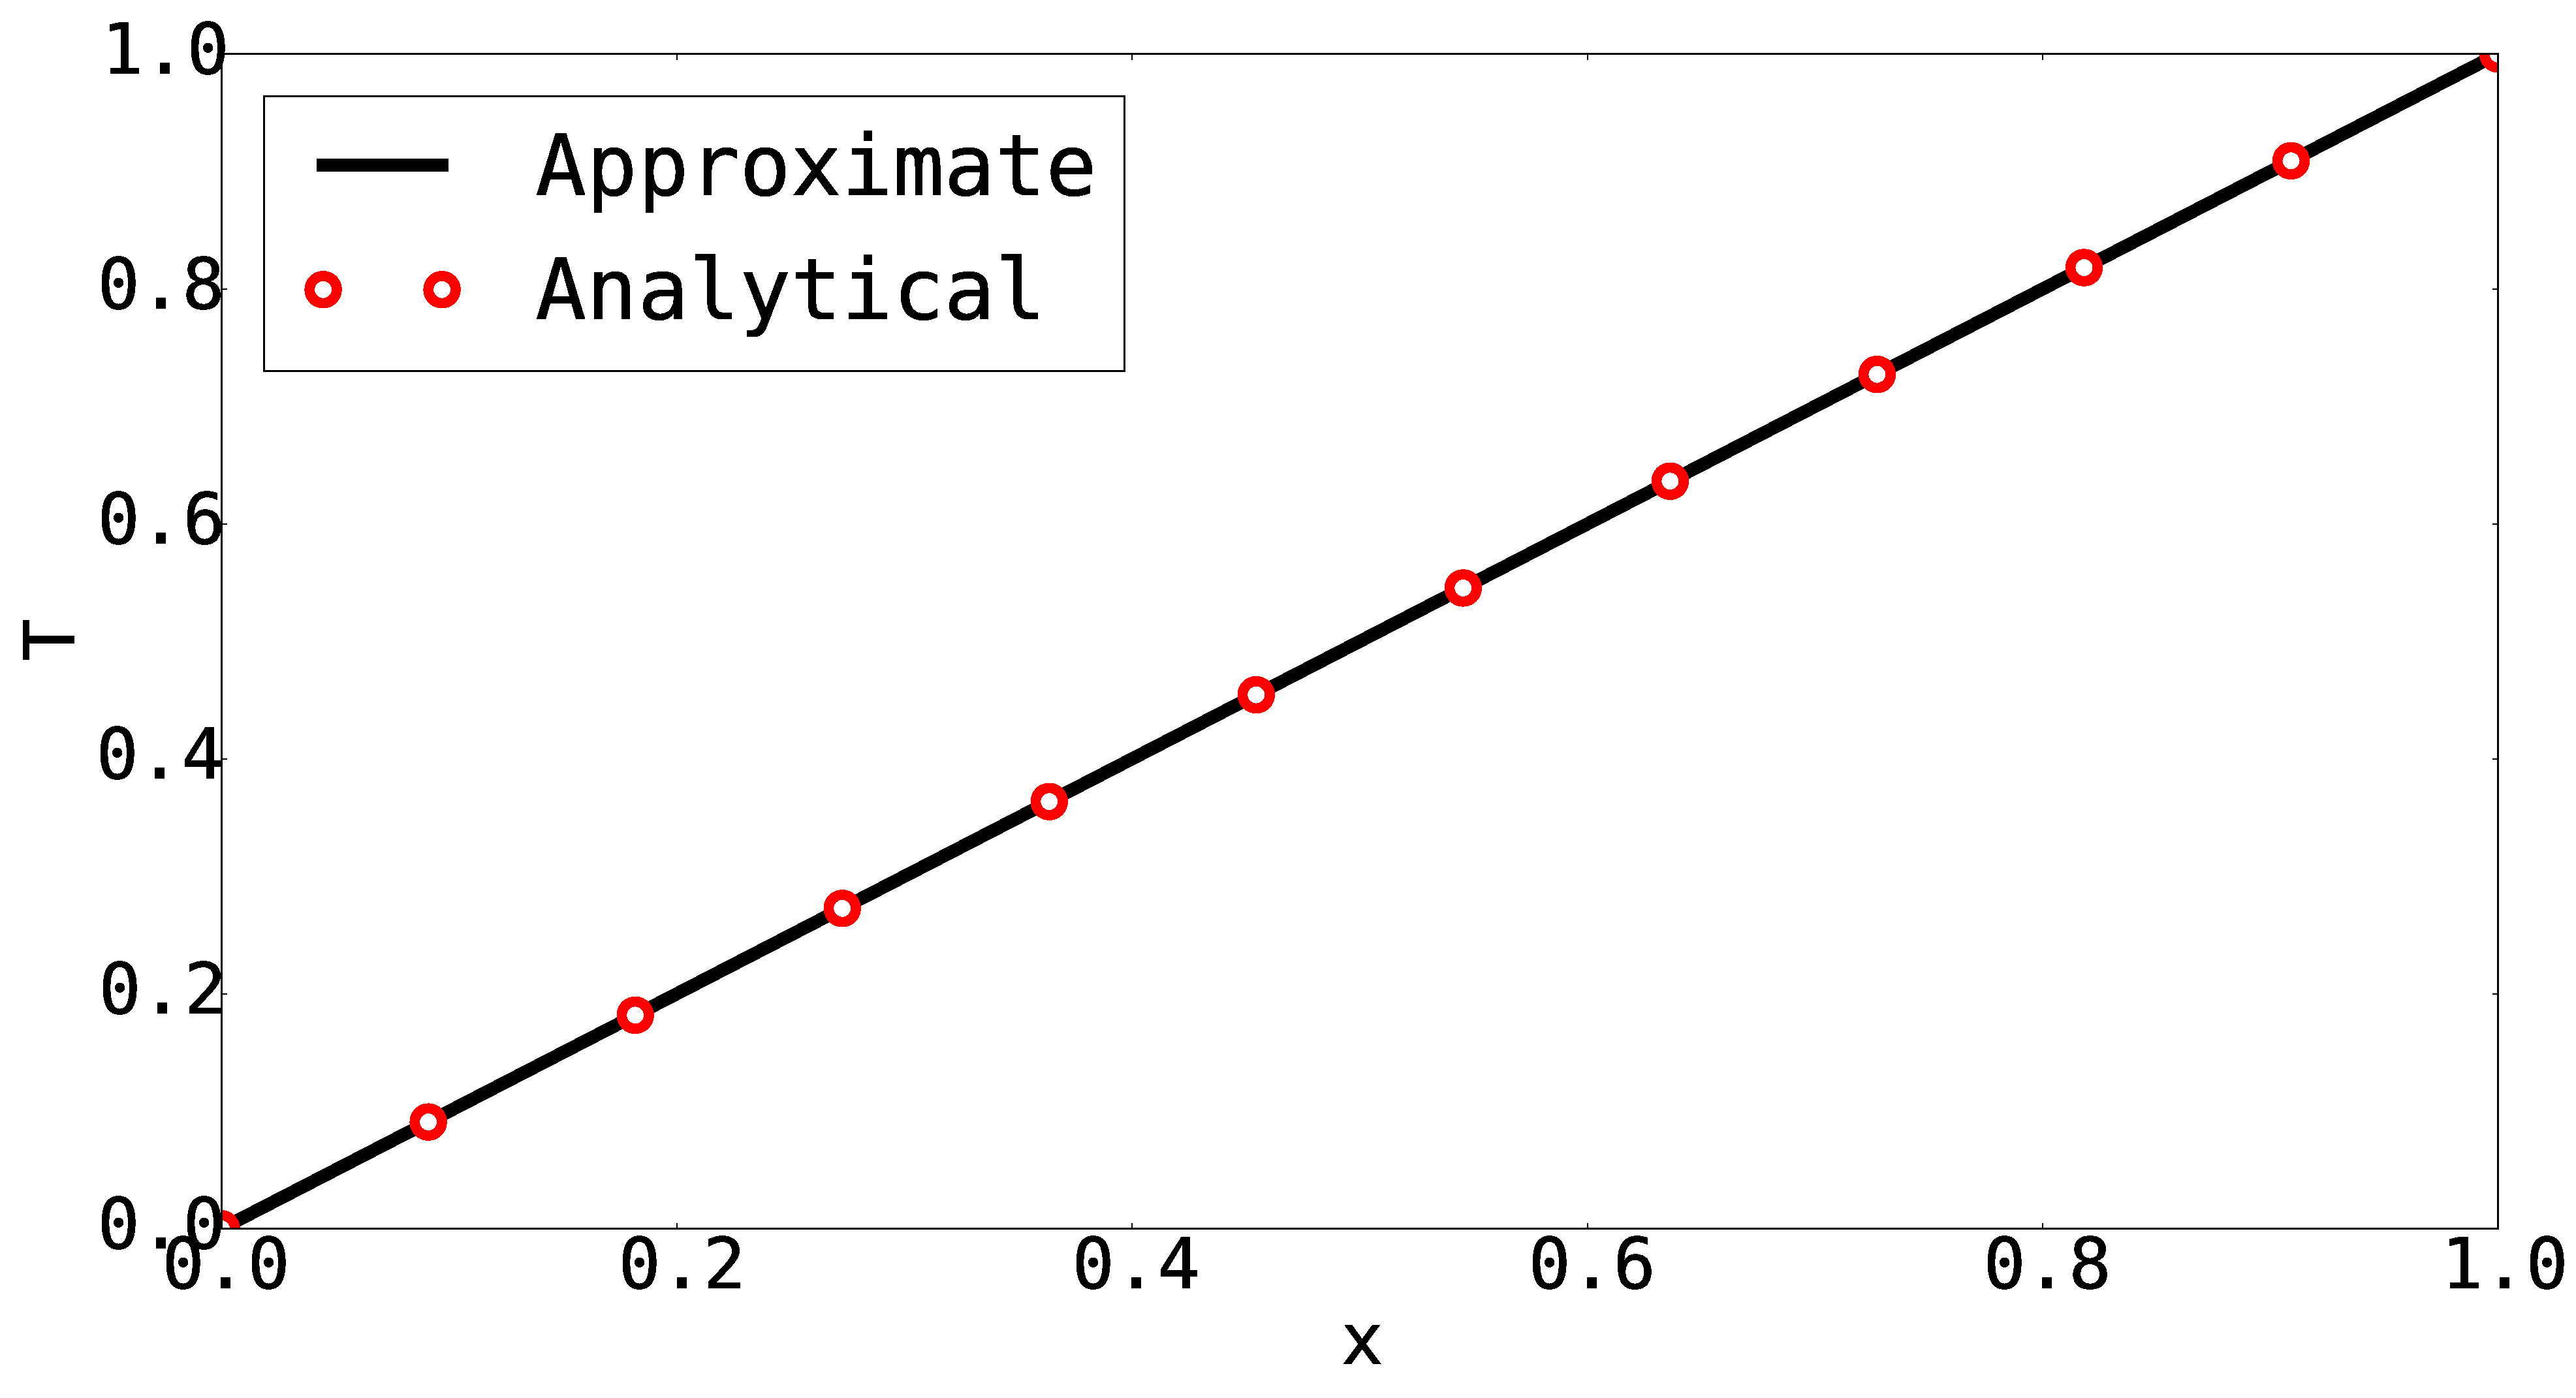
\includegraphics[width=7.0cm]{Chapter_2/figure/finitedifference_vs_analytical_n12.eps}
	}
	\\
	\subfigure[$n = 24$]
	{
	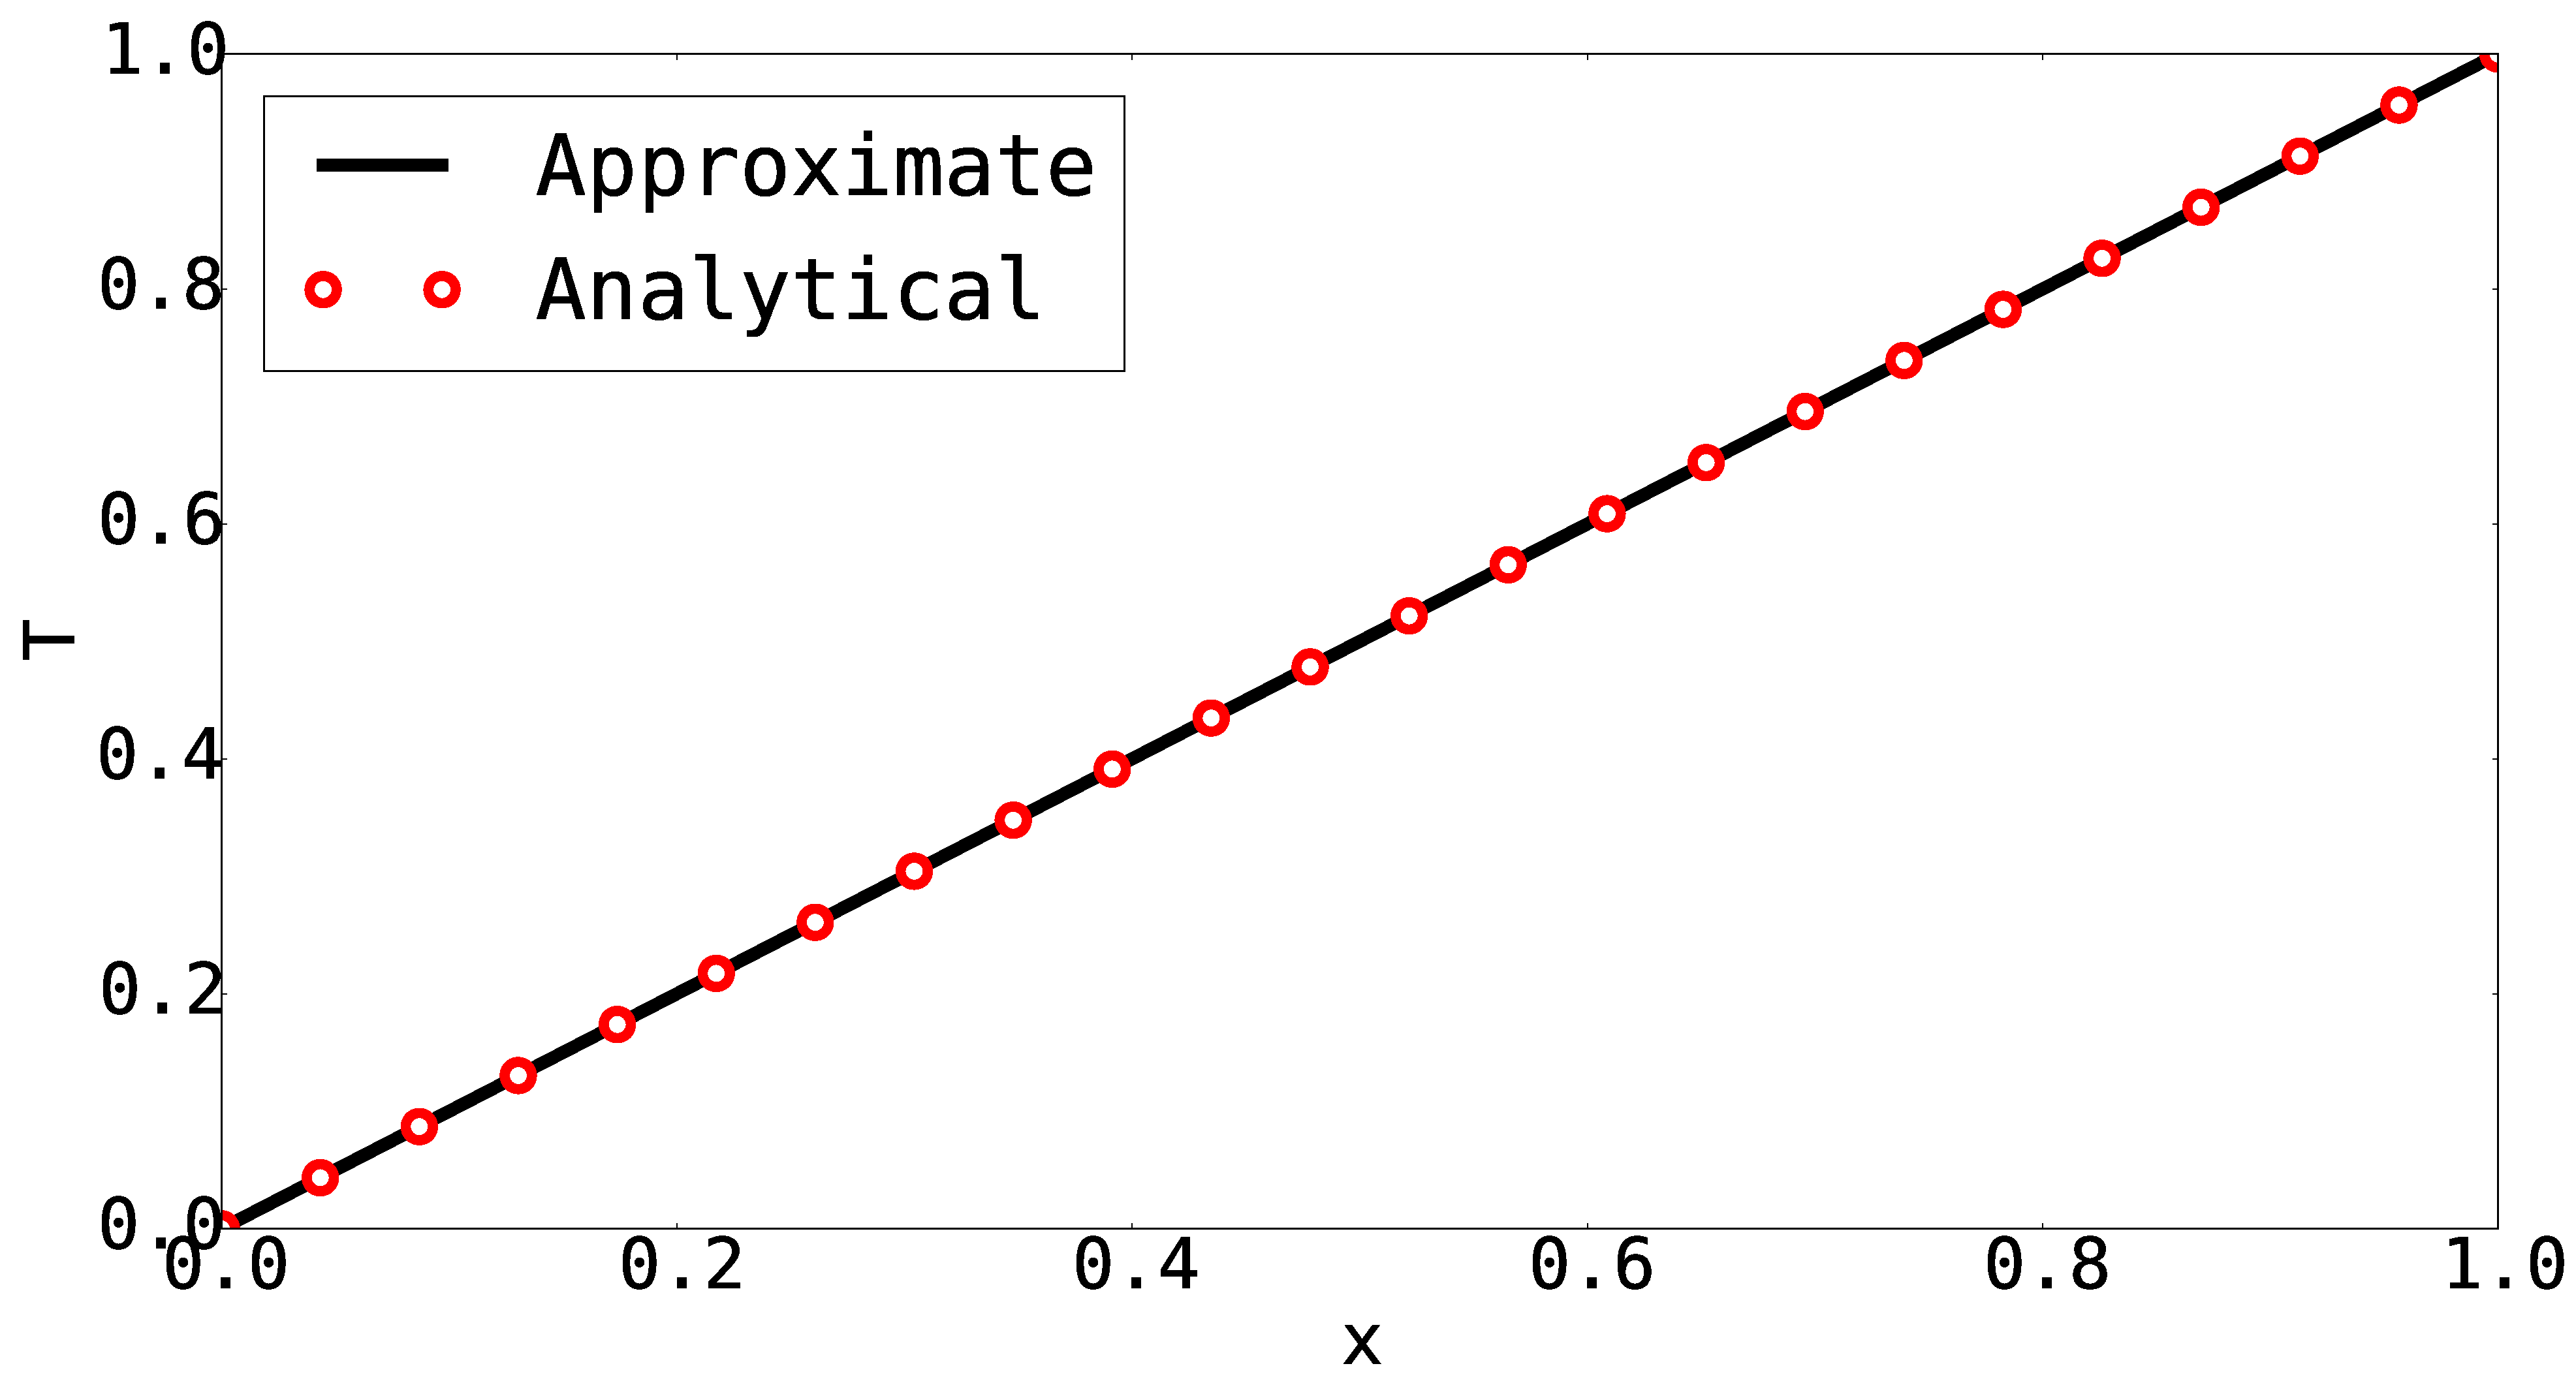
\includegraphics[width=7.0cm]{Chapter_2/figure/finitedifference_vs_analytical_n24.eps}
	}
	\quad
	\subfigure[$n = 48$]
	{
	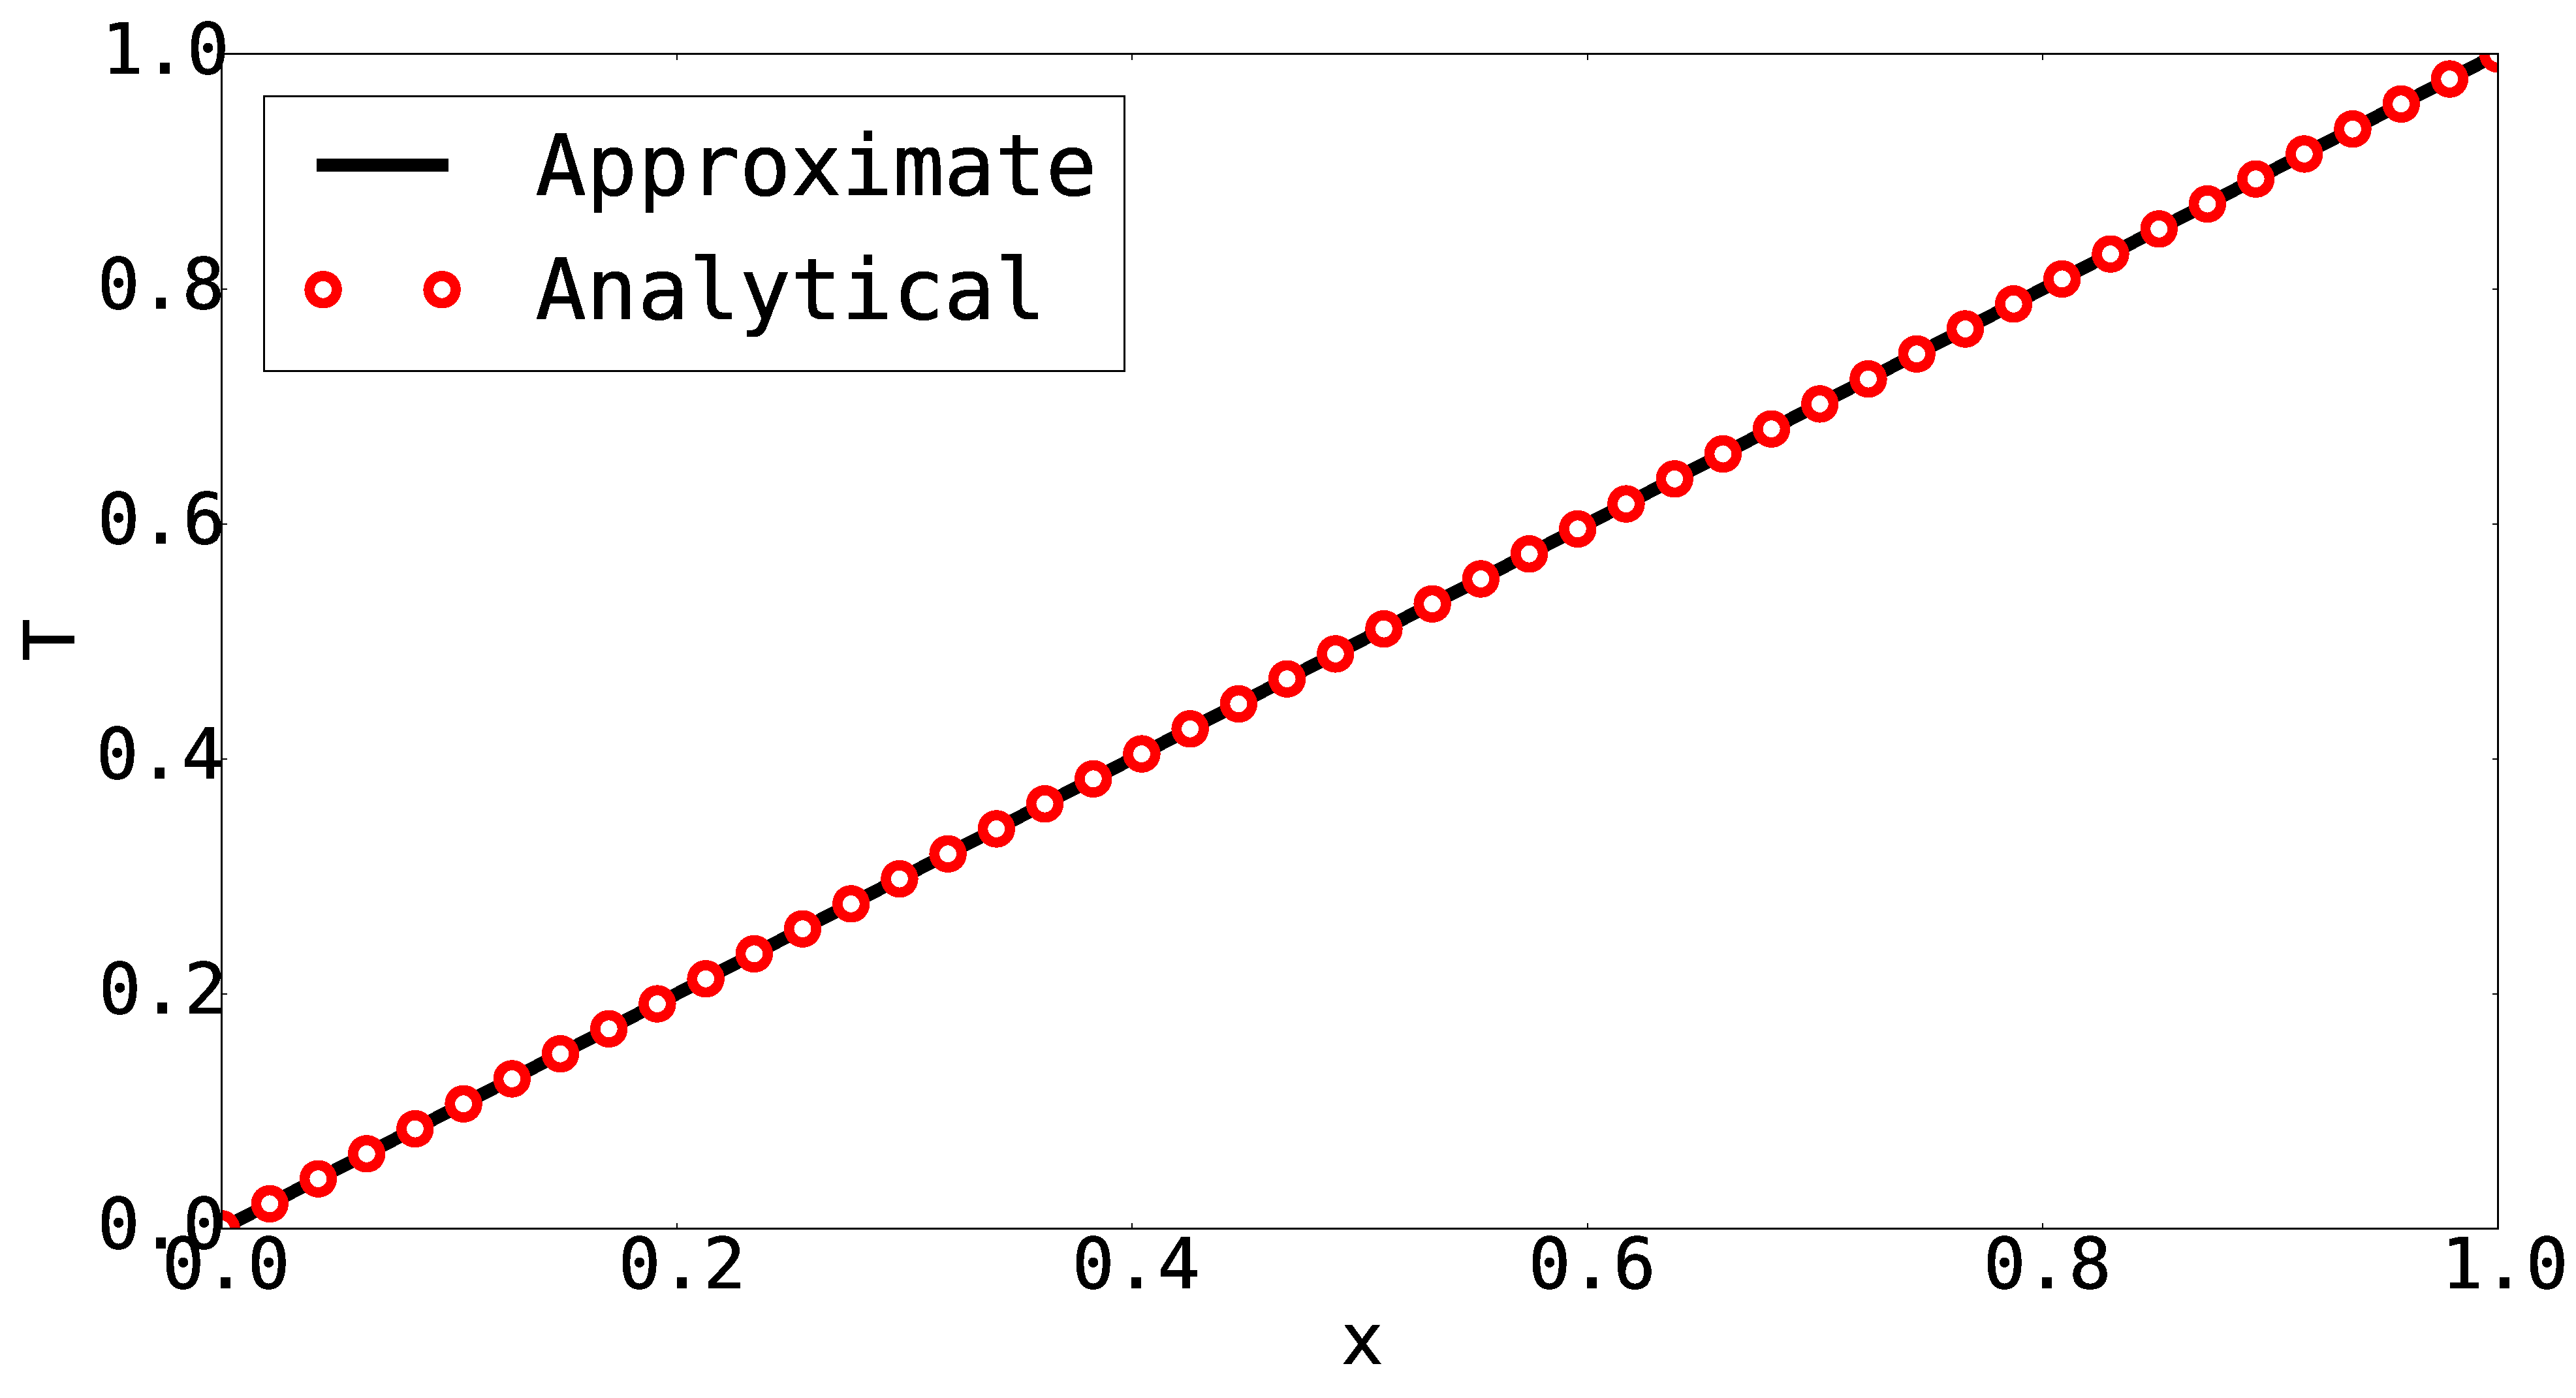
\includegraphics[width=7.0cm]{Chapter_2/figure/finitedifference_vs_analytical_n48.eps}
	}
	\caption{Comparison between the analytical and finite difference solutions for 1D heat equation for different number of nodes.}
	\label{fig:C2_verificationOfSolver}
\end{figure}

\begin{table}[H]
\centering
\begin{tabular}{| c | c |}
	\hline
	Number of nodes & absolute error \\ \hline \hline
	6 & $1.85 \times 10^{-16}$ \\ \hline
	12 & $2.03 \times 10^{-16}$ \\ \hline
	24 & $1.27 \times 10^{-15}$ \\ \hline
	48 & $8.55 \times 10^{-15}$ \\ \hline
\end{tabular}
\caption{Absolute error value for different number of nodes.}
\label{table:C2_solutionError}
\end{table}

The discrete sensitivity equations are derived by differentiating the discretized governing equation of \eqref{eq:C2_laplaceEquationMatrixForm} with respect to the length of the domain. We assume that the change in the length, only affects the nodal distance between the last two nodes and the rest remain unchanged. This means that only the node next to the boundary will move and the rest of nodes will be stationary. This is required to make sure that the sensitivity at each of the degrees of freedom is only a function of change in shape not movement of material nodes therefore, $\partial x/\partial b$ is equal to zero.

In order to differentiate Equation  \eqref{eq:C2_laplaceEquationMatrixForm}, it is required to calculate the derivative of nodal distances in Equation \eqref{eq:C2_laplaceEquationMatrixForm} with respect to $L$, $\partial \Delta_i/\partial L$. For an equally spaced grid, the nodal distance is written as

\begin{equation*}
	\Delta = \frac{L}{n - 1}
\end{equation*}

where $L$ is the length of the domain, and $n$ is the number of nodes used to discretize the domain. Therefore, the sensitivity of nodal distances to the length of the domain is calculated as

\begin{equation}\label{eq:C2_nodeDistanceSensitivity}
	\frac{\partial \Delta}{\partial L} = \frac{1}{n-1}
\end{equation}

The differentiated form of the discretized equation is written as shown in Equation \eqref{eq:C2_laplaceEquationMatrixFormSensitivity}. It should be noted that since only the adjacent node to the boundary is affected by shape change, only that element in the matrix derivative has a value.

\begin{equation}\label{eq:C2_laplaceEquationMatrixFormSensitivity}
	\begin{bmatrix}
		-2 & 1 & 0 & 0 \\
		1 & -2 & 1 & 0 \\
		0 & 1 & -2 & 1 \\
		0 & 0 & 1 & -2
	\end{bmatrix}
	\begin{bmatrix}
		T'_2 \\
		T'_3 \\
		T'_4 \\
		T'_5
	\end{bmatrix}
	=
	\frac{1}{2} \frac{\partial \Delta}{\partial L} \frac{1}{\Delta}
	\begin{bmatrix}
		0 \\
		0 \\
		0 \\
		T_6
	\end{bmatrix}
	-
	\underbrace{
	\frac{1}{2} \frac{\partial \Delta}{\partial L} \frac{1}{\Delta}
	\begin{bmatrix}
		0 & 0 & 0 & 0 \\
		0 & 0 & 0 & 0 \\
		0 & 0 & 0 & 0 \\
		0 & 0 & -3 & 1
	\end{bmatrix}
	\begin{bmatrix}
		T_2 \\
		T_3 \\
		T_4 \\
		T_5
	\end{bmatrix}}_\text{effect of shape change}
\end{equation}

where $T^\prime_i$ represents the sensitivity of temperature with respect to length of the domain. In order to better study Equation \eqref{eq:C2_laplaceEquationMatrixFormSensitivity}, we mention the general sensitivity equation in a discrete form. Assume the continuum governing equation \eqref{eq:C2_generalGoverningEquation}, is be written in the discrete form as

\begin{equation}
	\left[ K \right] \left[ U \right] = \left[ F \right]
\end{equation}

where $[K]$ is the discrete operator that represents the governing equation, $[U]$ is the vector of response variables defined at each of the degrees of freedom, and $[F]$ is the vector of the boundary conditions. The sensitivity of this system with respect to design variable $b$ is derived as

\begin{equation}\label{eq:C2_discreteSensitivityEquation}
	\left[ K \right] \left[ \frac{\partial U}{\partial b} \right] = 
	\left[ \frac{\partial F}{\partial b} \right] - 
		\left[ \frac{\partial K}{\partial b} \right] \left[ U \right]
\end{equation}

By comparing Equation \eqref{eq:C2_discreteSensitivityEquation} with Equation \eqref{eq:C2_laplaceEquationMatrixFormSensitivity}, we can see that the last term represents the change in the stiffness matrix. This depends on how the governing equations are discretized. Therefore, to do the sensitivity analysis it is required to know how this matrix is derived so it can be differentiated. This is not possible in most cases since the details of discretization are not known for the commertial software packages.

To verify the results of Equation \eqref{eq:C2_laplaceEquationMatrixFormSensitivity}, we compared it with the analytical sensitivity results as shown in Figure \ref{fig:C2_discreteSensitivityVerification}. We discretized the domain using $11$, $41$, $81$, and $161$ nodes for this purpose, however this does not affect the solution accuracy. We chose the normalized root-mean-square deviation (NRMSD) for comparing the sensitivity results. This is defined as shown in Equation \eqref{eq:C2_NRMSD}.

\begin{equation}\label{eq:C2_NRMSD}
	NRMSD = \dfrac{\sqrt{\dfrac{\sum (\hat{y}_t - y)^2}{n}}}{y_{max} - y_{min}}
\end{equation}

where $\hat{y}$ is the value calculated using DSA and $y$ is the true value calculated by analytical equation. The results for the NRMSD for this problem for different number of nodes are shown in Table \ref{table:C2_DSA_NRMSD}.

\begin{figure}[H]
	\centering
	\subfigure[$n = 11$]
	{
	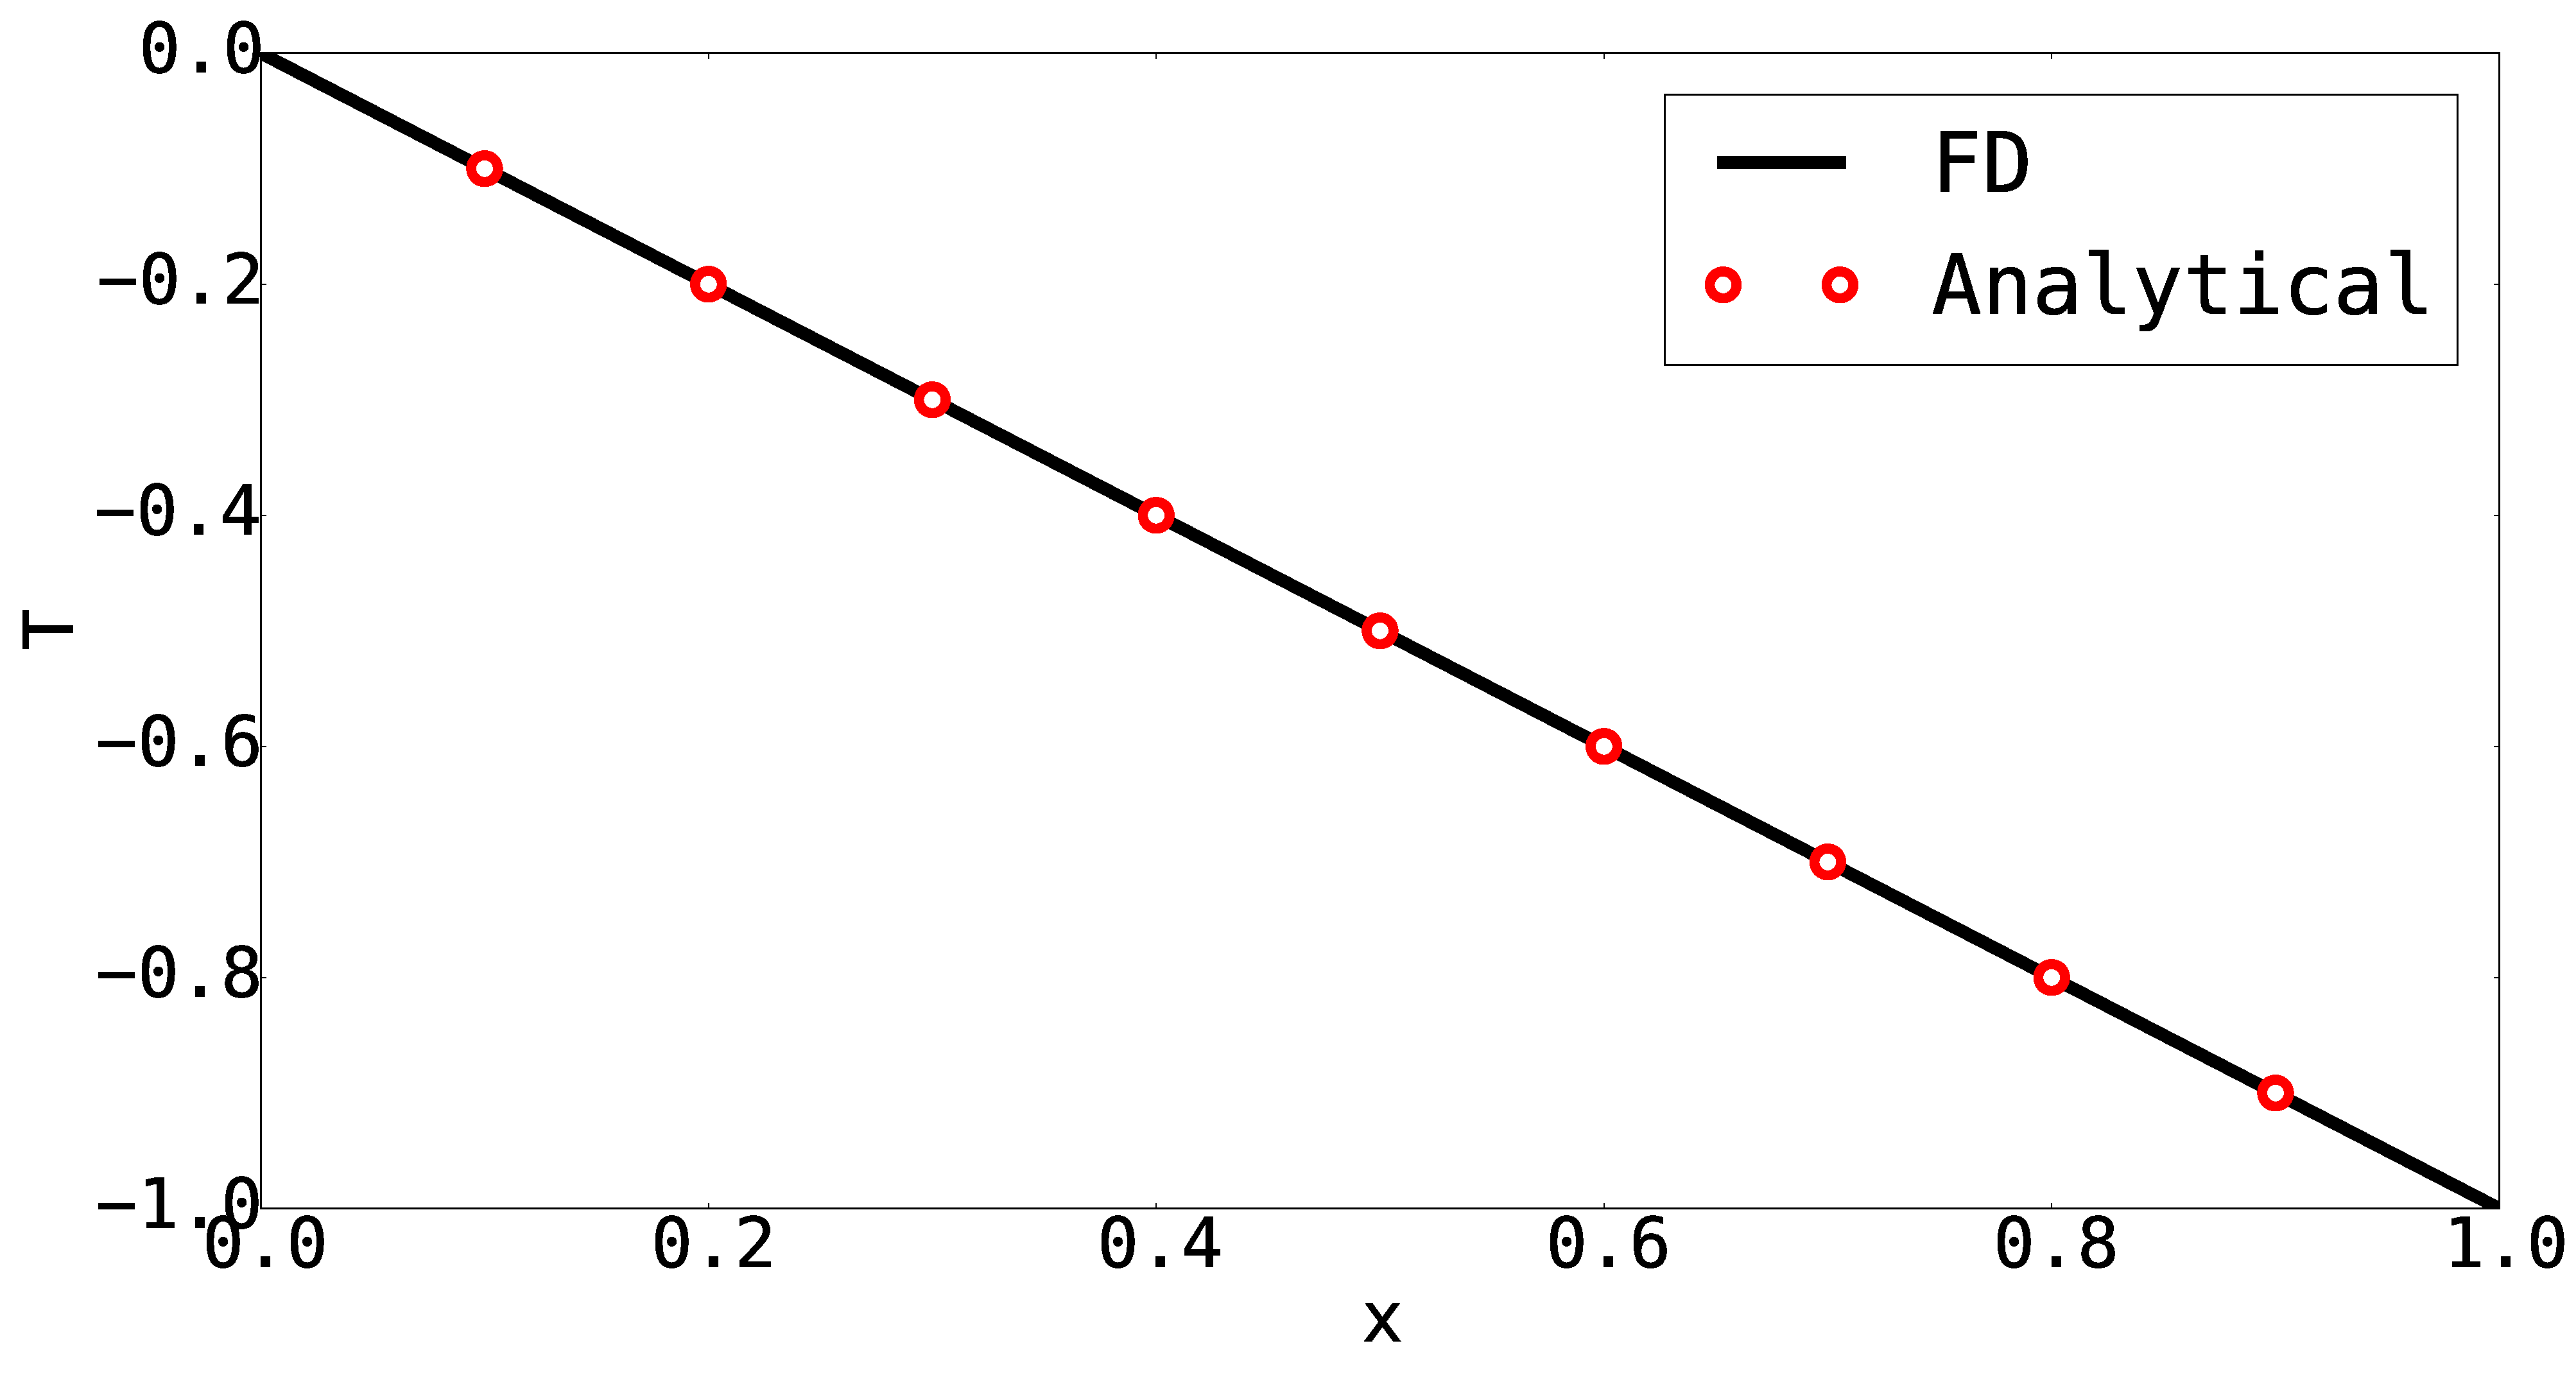
\includegraphics[width=7.0cm]{Chapter_2/figure/DSA_n11.eps}
	}
	\quad
	\subfigure[$n = 41$]
	{
	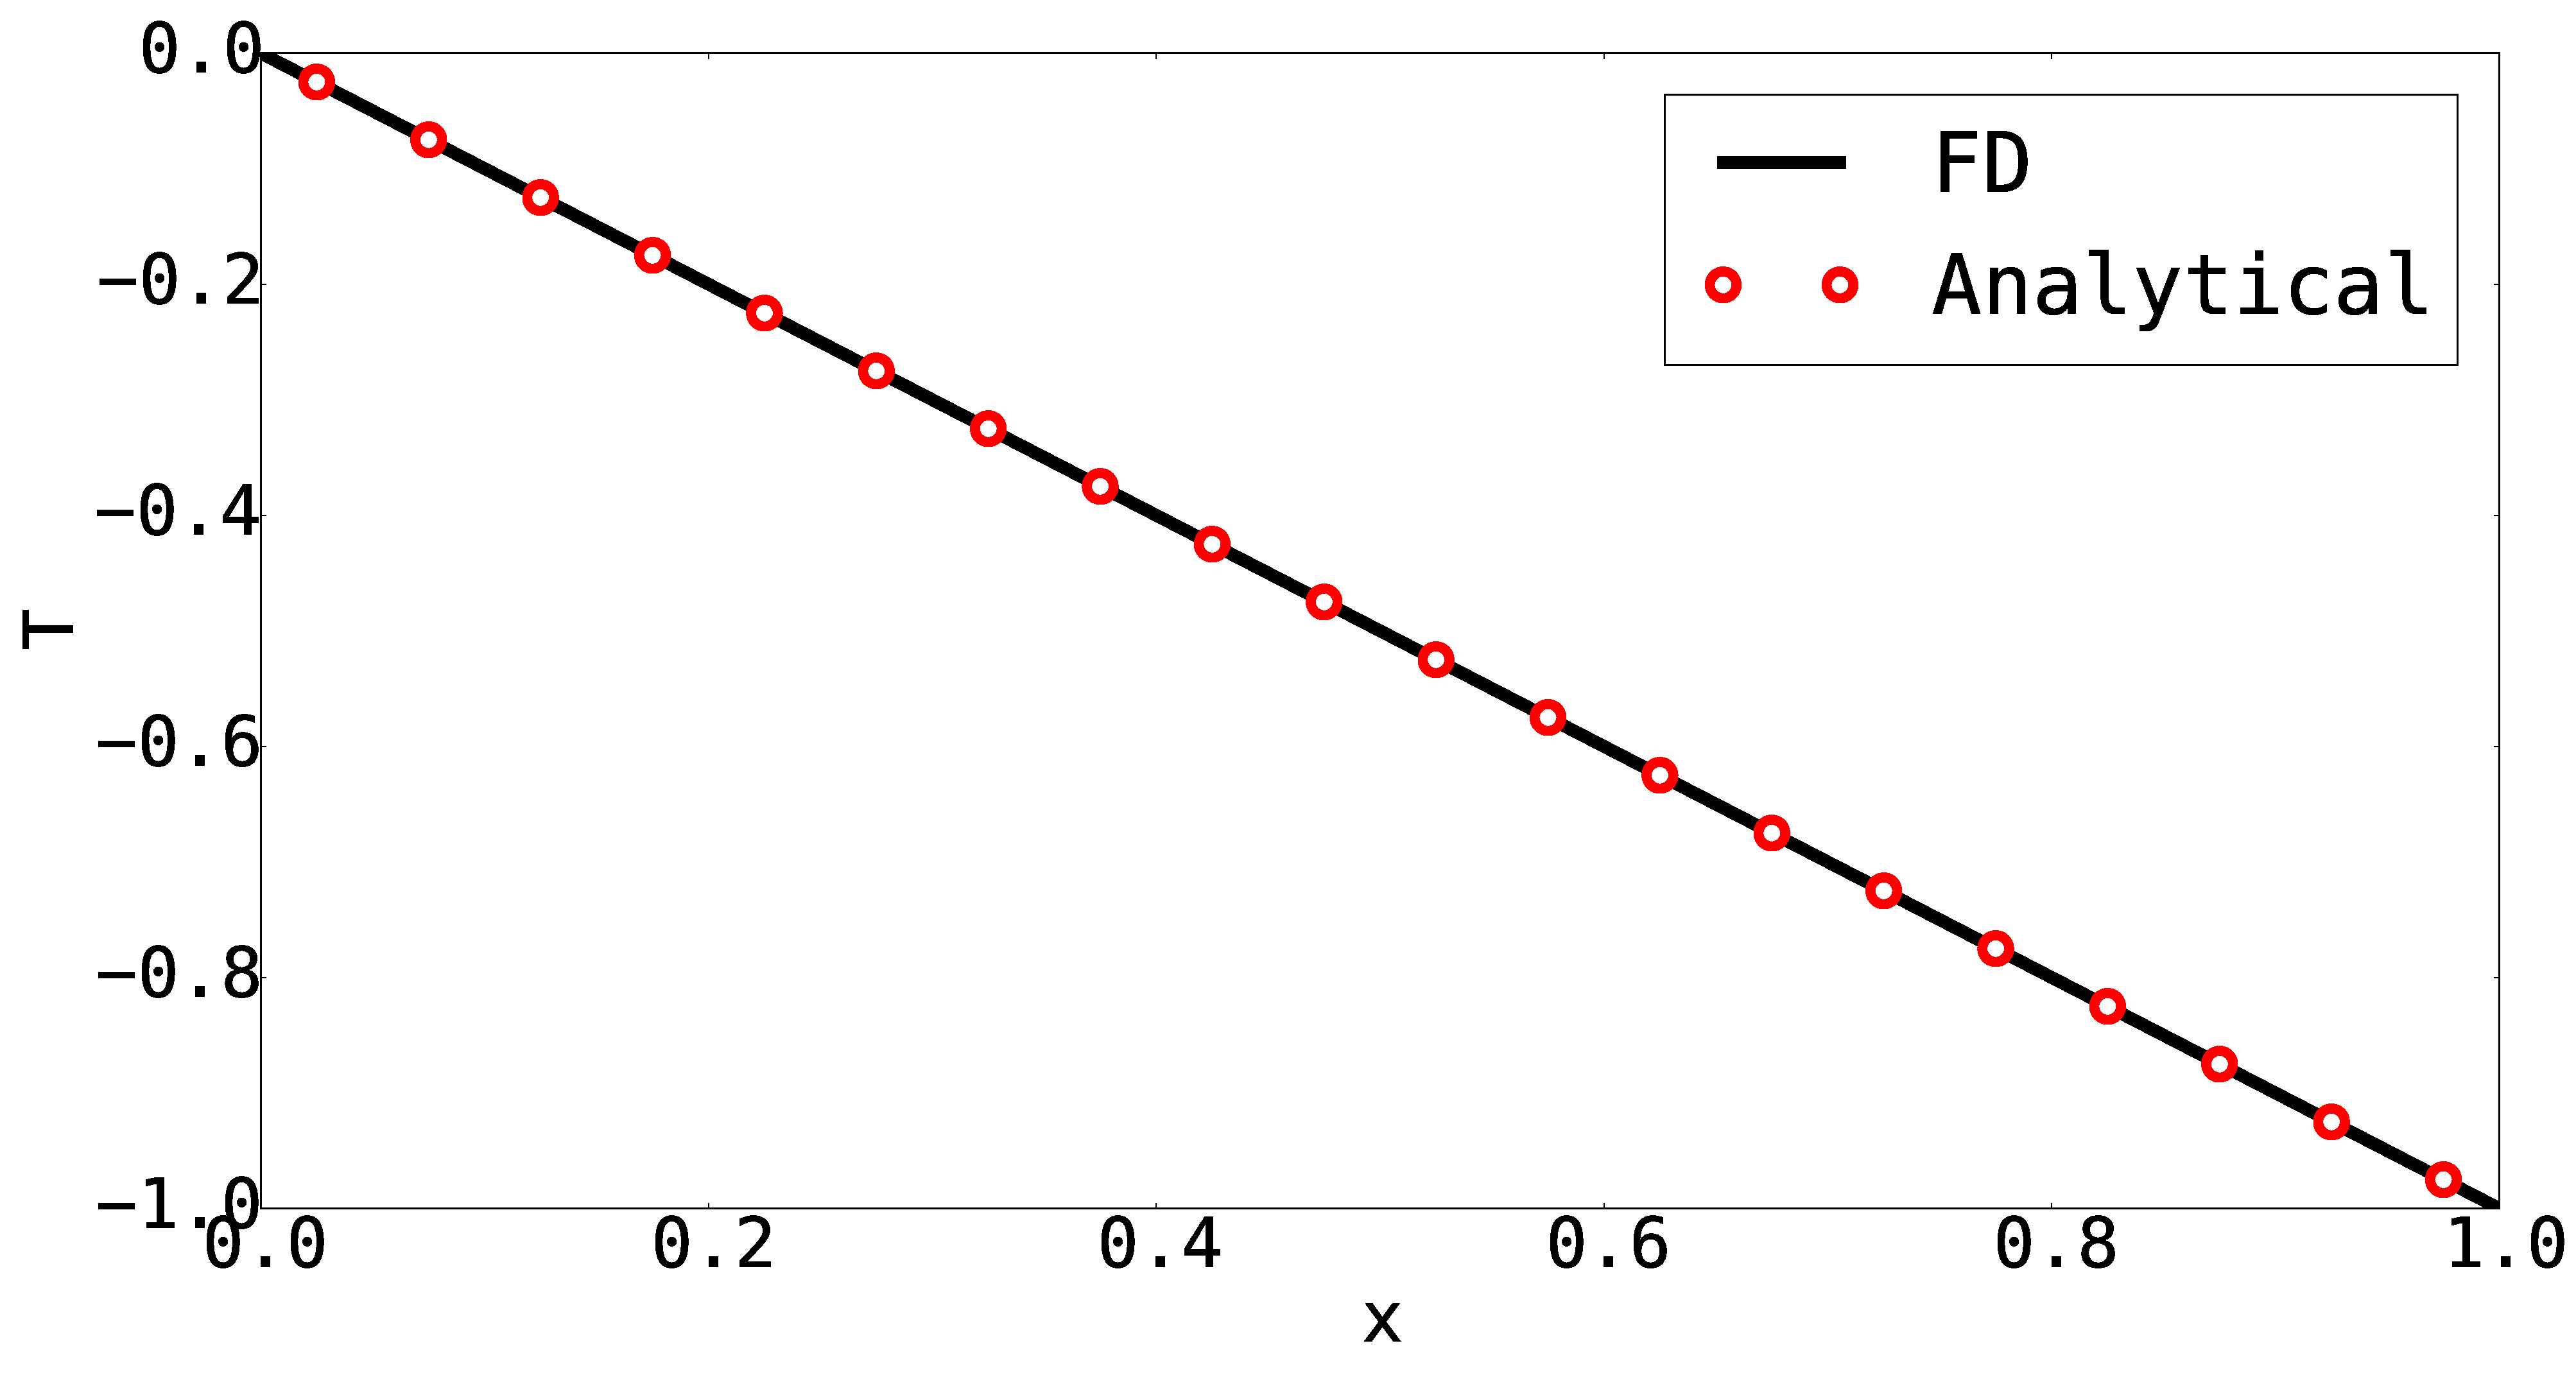
\includegraphics[width=7.0cm]{Chapter_2/figure/DSA_n41.eps}
	}
	\\
	\subfigure[$n = 81$]
	{
	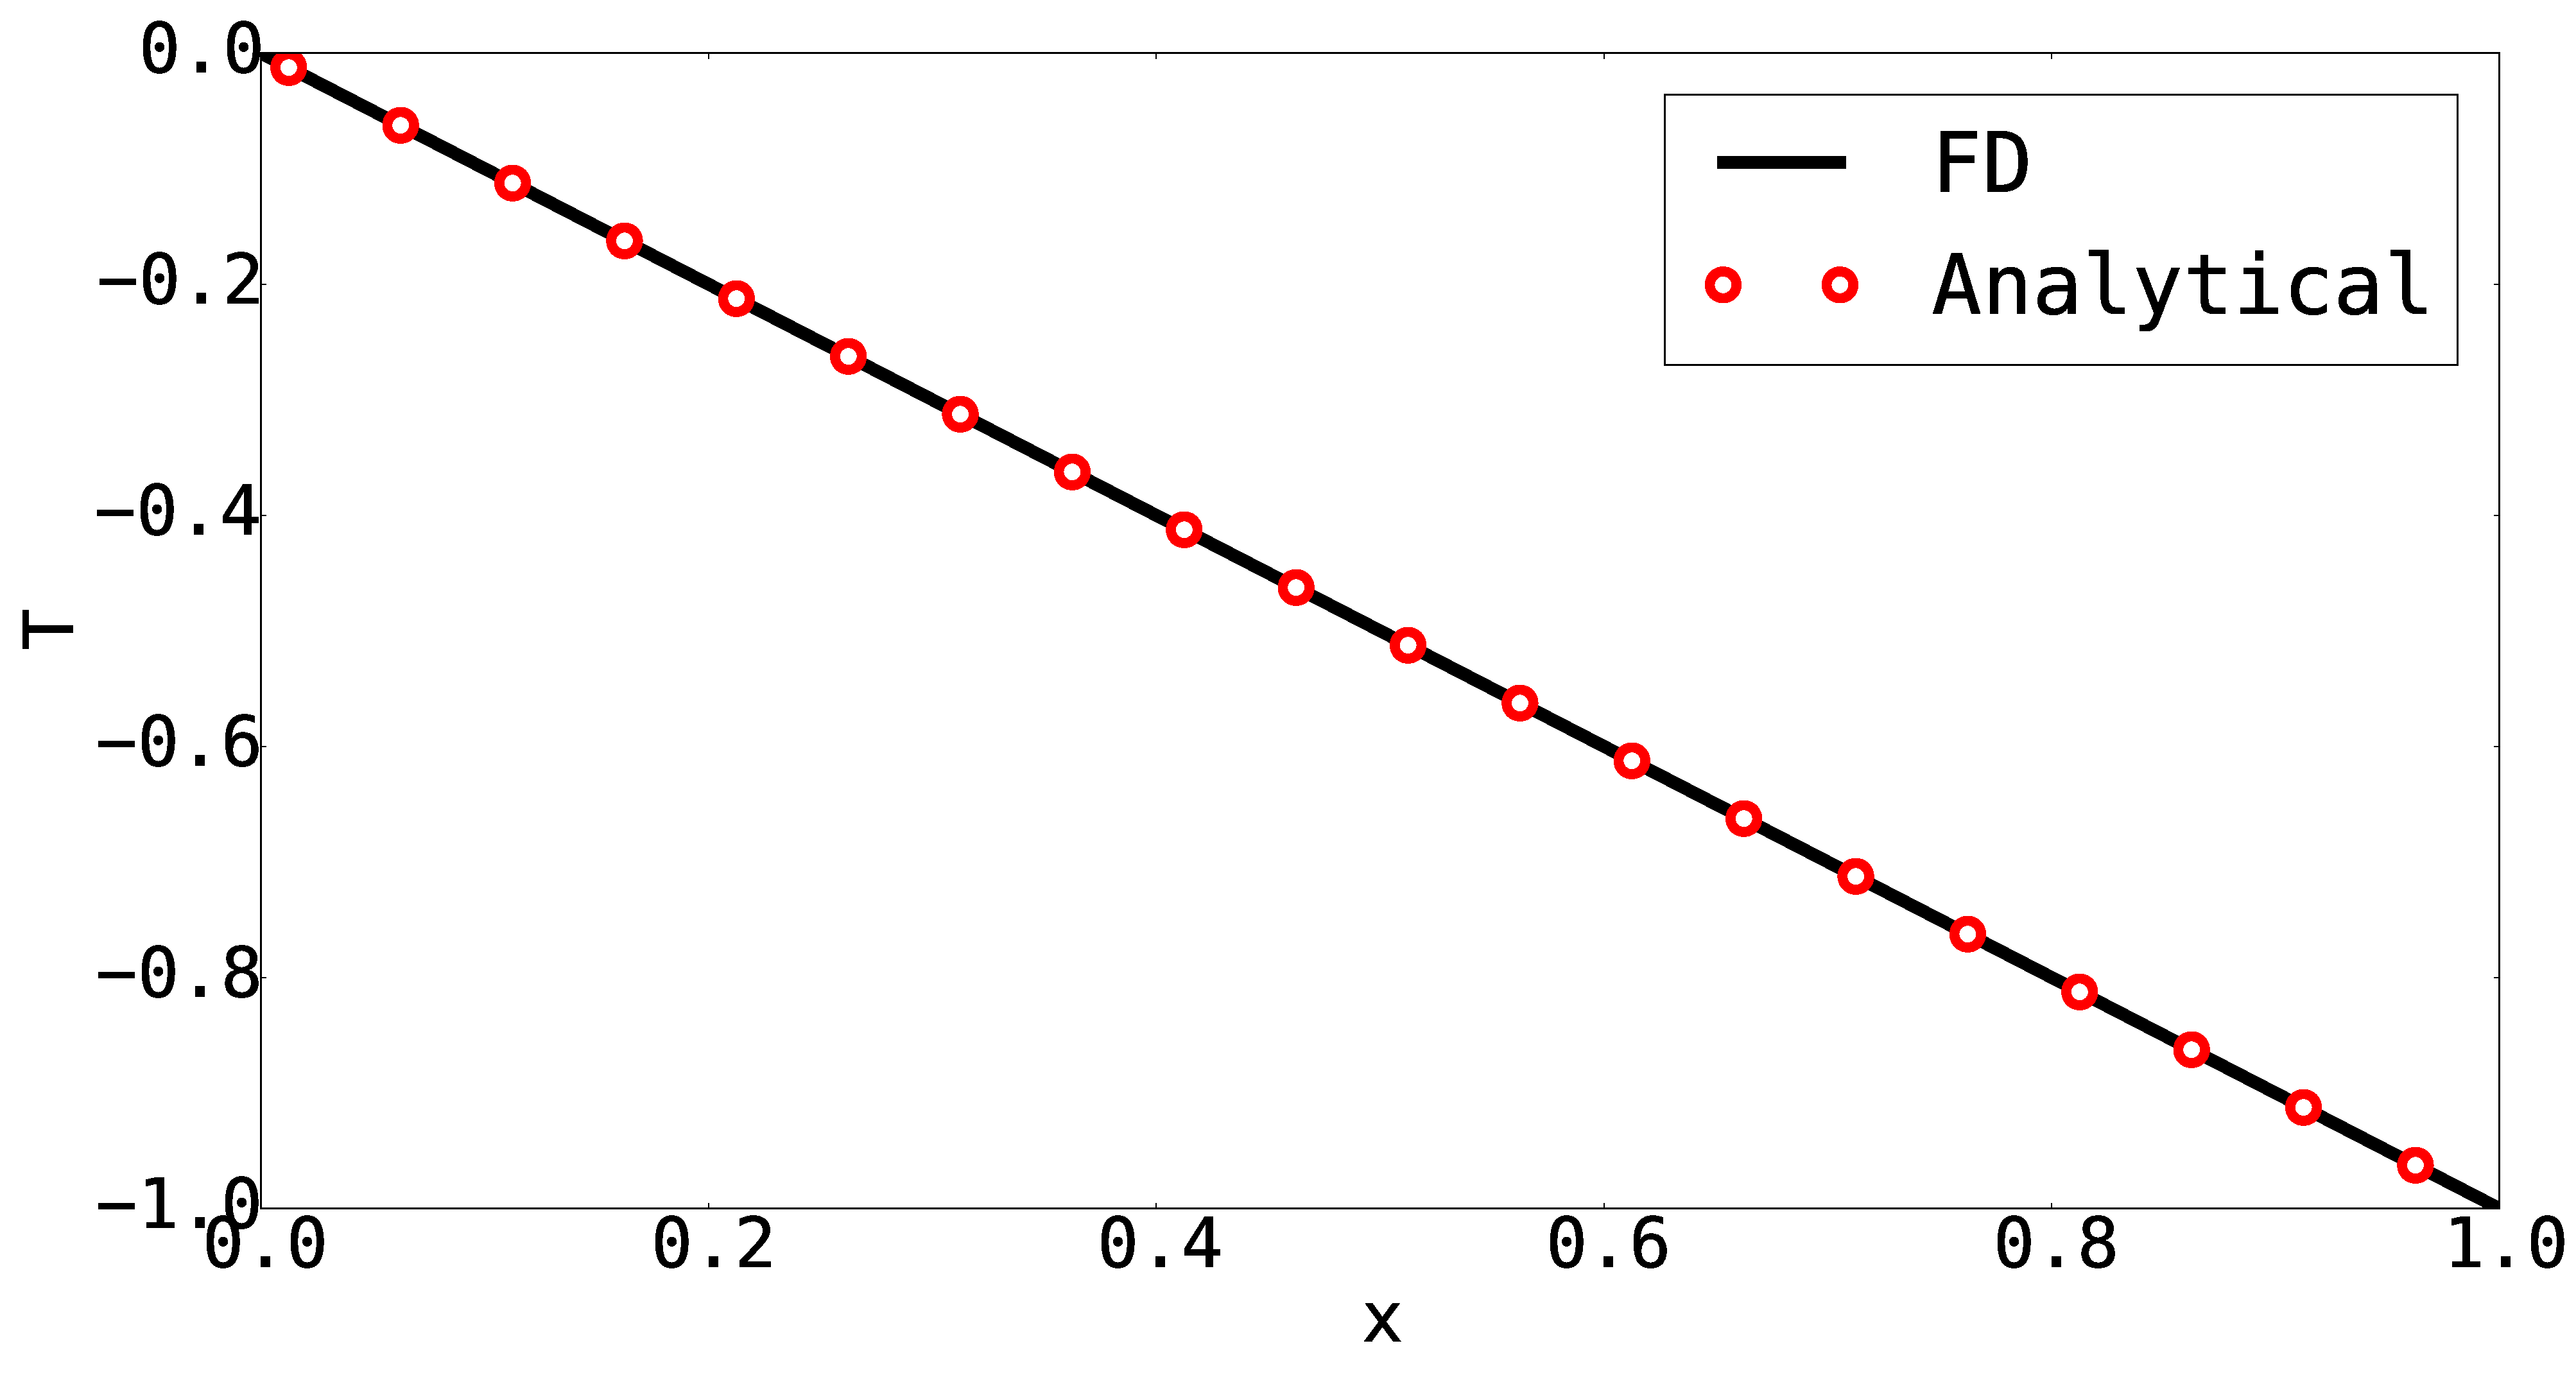
\includegraphics[width=7.0cm]{Chapter_2/figure/DSA_n81.eps}
	}
	\quad
	\subfigure[$n = 161$]
	{
	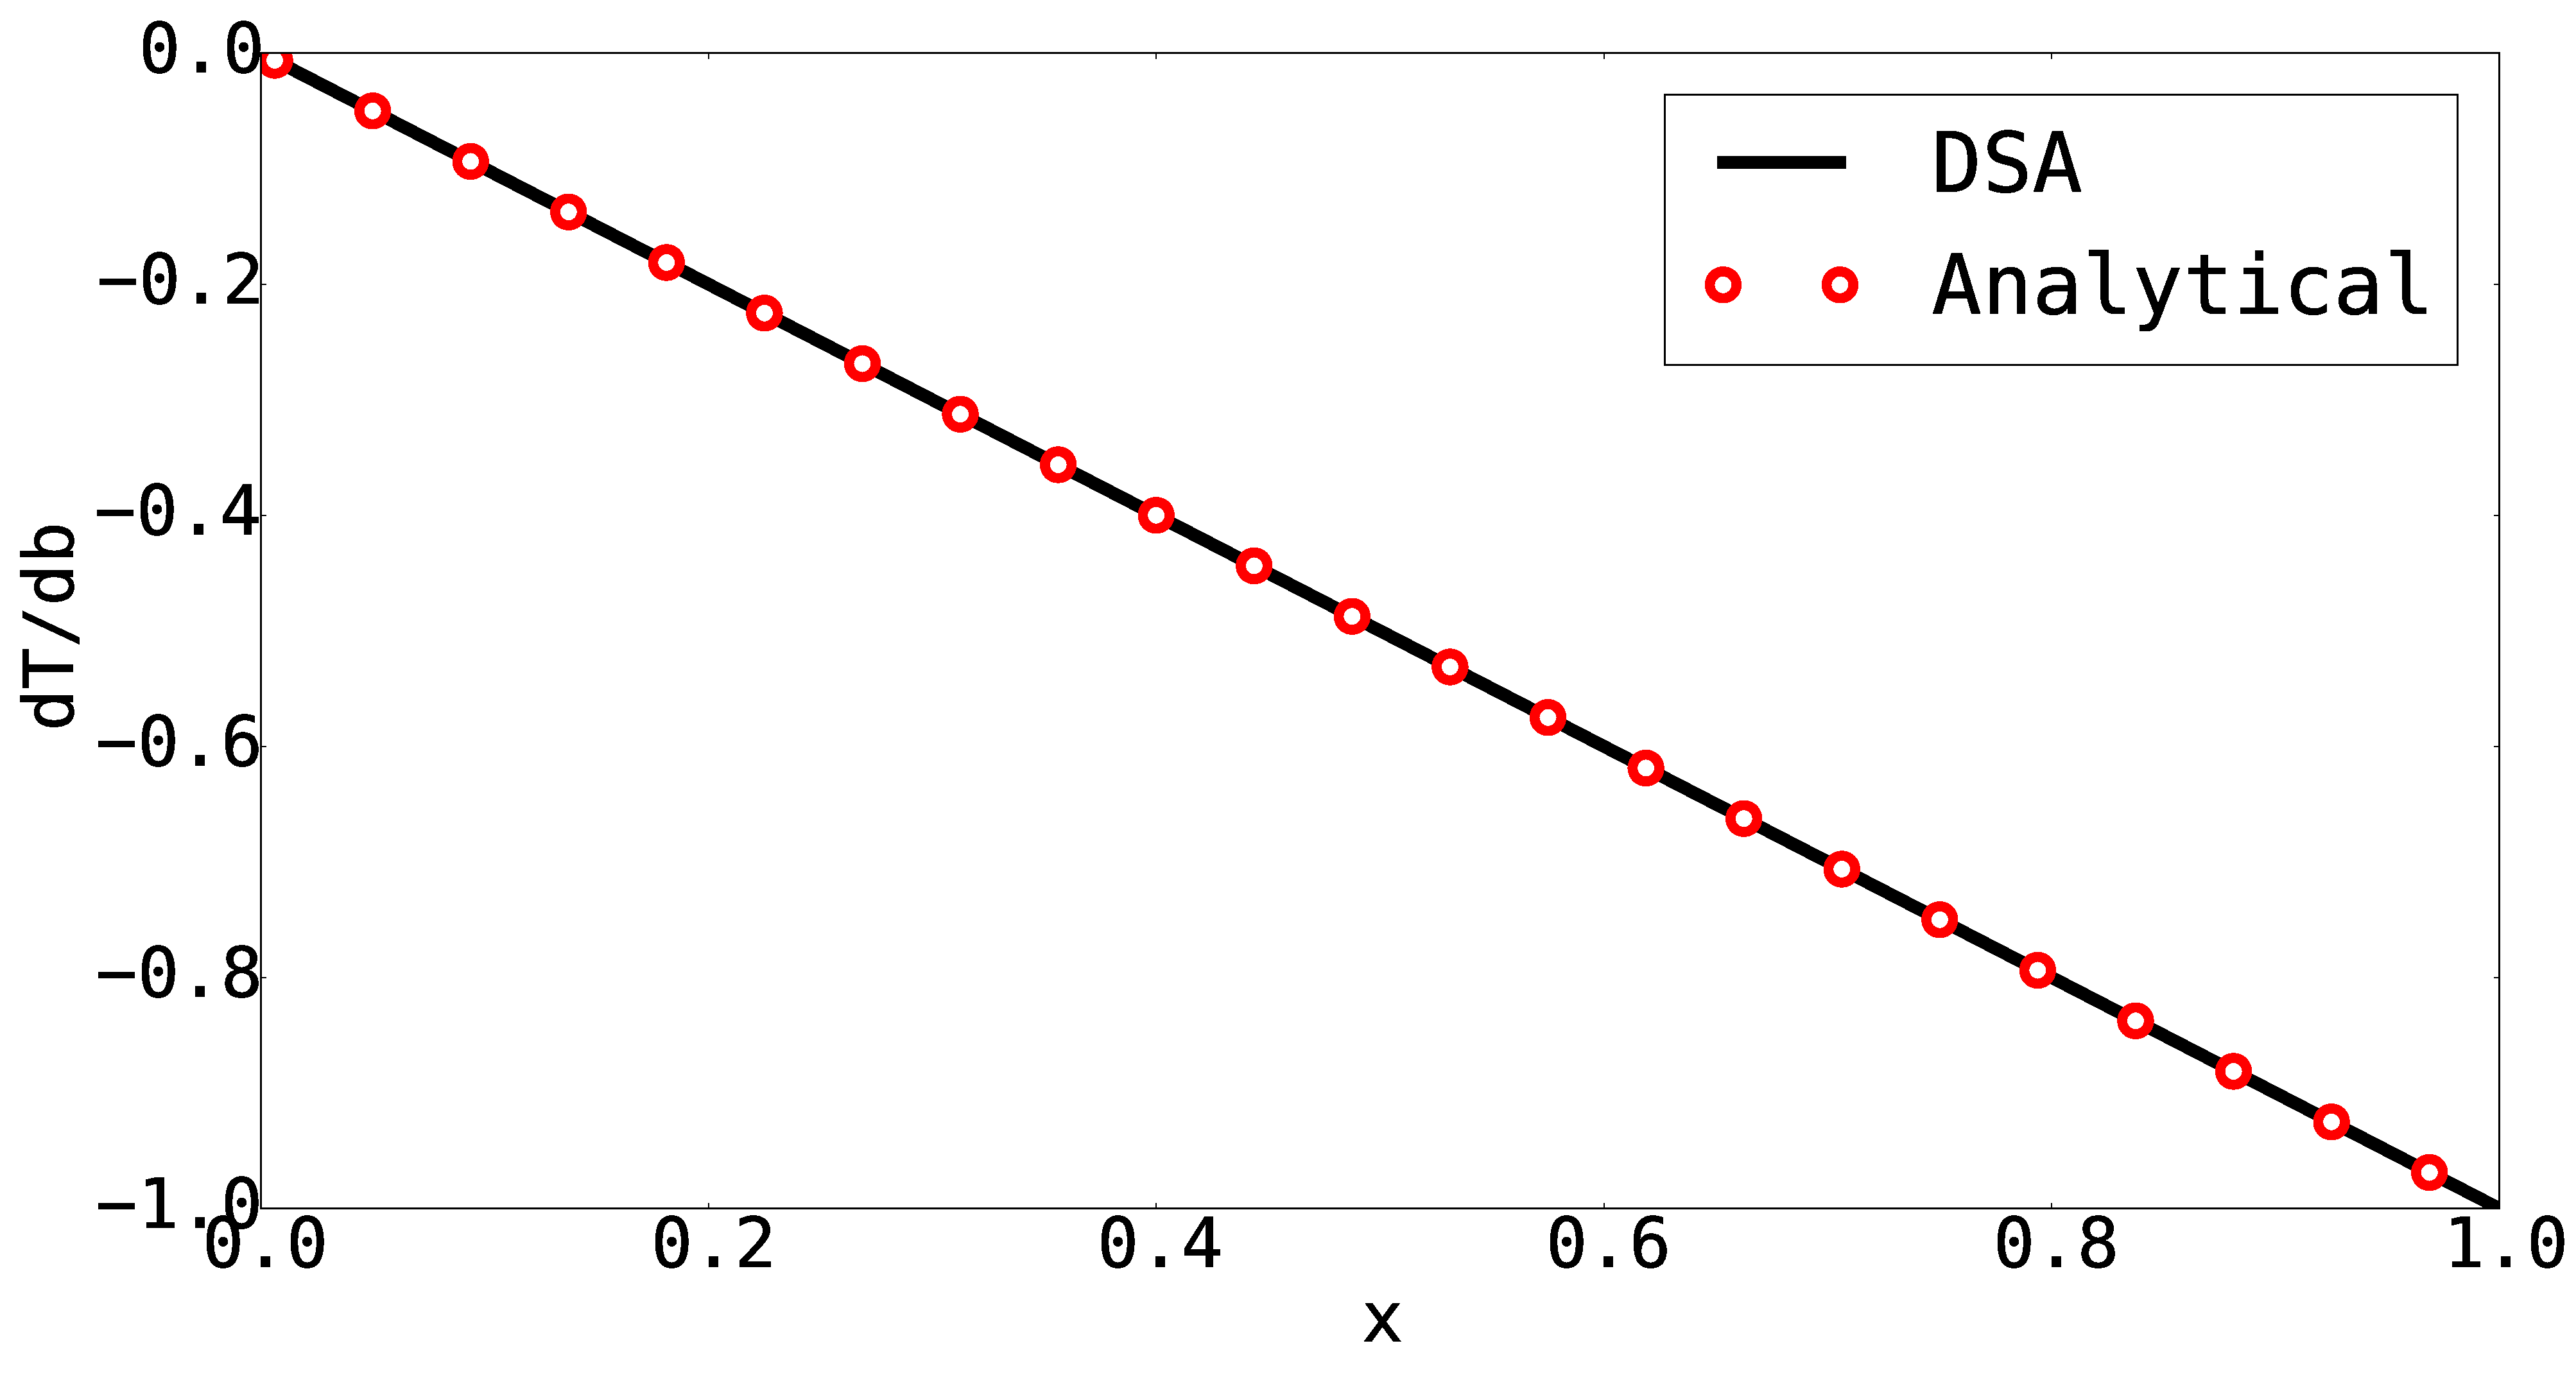
\includegraphics[width=7.0cm]{Chapter_2/figure/DSA_n161.eps}
	}
	\caption{Comparison between discrete sensitivity analysis and analytical results for different number of nodes.}
	\label{fig:C2_discreteSensitivityVerification}
\end{figure}

\begin{table}[H]
\centering
\begin{tabular}{| c | c |}
	\hline
	Number of nodes & NRMSD \\ \hline \hline
	11 & $1.68 \times 10^{-16}$ \\ \hline
	41 & $2.49 \times 10^{-15}$ \\ \hline
	81 & $1.49 \times 10^{-15}$ \\ \hline
	161 & $2.85 \times 10^{-15}$ \\ \hline
\end{tabular}
\caption{RMSE value for different number of nodes.}
\label{table:C2_DSA_NRMSD}
\end{table}

As shown in Figure \ref{fig:C2_discreteSensitivityVerification} and Table \ref{table:C2_DSA_NRMSD}, the accuracy of discrete sensitivity analysis is not affected by the number of nodes chosen to discretize the domain.

% ======================================================================================
\section{Continuum Sensitivity Formulation}
For a continuous system, the governing equations and boundary conditions are written as

\begin{subequations}\label{eq:C2_continuumGoverningEquation}
\begin{align}
	A(u, t; b) &= 0 \qquad \qquad \text{on } \Omega \\
	B(u, t; b) &= g(x, t; b) \quad \text{on } \Gamma
\end{align}	
\end{subequations}

where $u$ is the response variable, i.e. displacement or pressure, $t$ is time, $x$ is the spatial coordinate, and $b$ is the design variable that can be used to control the solution. $A$ and $B$ are continuum functions that define the governing equations and boundary conditions respectively. It should be noted that the governing equation is written in the residual form where its value needs to be equal to zero when $u$ is the solution at time $t$. $g$ is the value of the boundary condition of the defined system. To calculate the sensitivity of response, it is required to calculate the total derivative of Equation \eqref{eq:C2_continuumGoverningEquation}. This is done by calculating the local sensitivity of the governing equation followed by converting the local sensitivities to their total form using Equation \eqref{eq:C2_totalSensitivityDef}.

The governing equation and the boundary condition of \eqref{eq:C2_continuumGoverningEquation} are differentiated as follows

\begin{subequations}\label{eq:C2_continuumSensitivityFormulation}
\begin{align}
	A(u', t; b) + A'(u, t; b) &= 0 \qquad \qquad \text{on } \Omega \\
	B(\dot{u}, t; b) + \dot{B}(u, t; b) &= \dot{g}(x, t; b) \quad \text{on } \Gamma
\end{align}	
\end{subequations}

where $(\text{ })'$ and $\dot{(\text{ })}$ are local and total derivative which are defined as follows

\begin{subequations}
\begin{align*}
	(\text{ })' &= \frac{\partial (\text{ })}{\partial b} \\
	\dot{(\text{ })} &= \frac{D (\text{ })}{D b}
\end{align*}
\end{subequations}

It should be noted that the governing equations are differentiated in the local form and the boundary conditions are differentiated in the total form. Local differentiation of the governing equations enables us to treat the solver non-intrusively \cite{cross2014local}. However, in order to capture the effect of shape change, the boundary conditions need to be differentiated in the total form. The boundary condition definition is further simplified by assuming linearly. This is a valid assumption for many practical cases such as structural analysis or computational fluid dynamics. The boundary conditions are usually in the form of known gradient or values, i.e. outflow and free-slip wall for CFD and predefined displacement/force for structural analysis. It should be noted that this assumption is not valid for problems such as contacts. The boundary condition is written as

\begin{align}\label{eq:C2_linearSAboundaryCondtions}
\begin{split}
	B(\dot{u}, t; b) &= \dot{g}(x, t; b) \Rightarrow \\
	B(u', t; b) &= \dot{g}(x, t; b) - B(\frac{\partial u}{\partial x} \cdot \frac{\partial x}{\partial b}, t; b)
\end{split}
\end{align}

To study the differentiated governing equation of Equation \eqref{eq:C2_continuumSensitivityFormulation}, we will assume two situations: i) linear analysis, ii) nonlinear analysis.

For the linear analysis, the governing  of \eqref{eq:C2_continuumSensitivityFormulation} is written as

\begin{equation}\label{eq:C2_linearSAgoverningEquation}
	A(u', t; b) = 0 
\end{equation}

This is valid since for the linear case, the differential operators of the governing equation do not depend on the response variable, $u$. To explain this concept, we look at the transient heat conduction in 1D domain. The governing equations are defined as

\begin{equation}\label{eq:C2_transientHeatCondtionGE}
	\frac{\partial^2 T}{\partial x^2} = \frac{1}{\alpha} \frac{\partial T}{\partial t}
\end{equation}

where $T$ is the temperature, $x$ is spatial coordinate, $t$ is time, and $\alpha$ is is the thermal diffusivity ($k/\rho c_p$). This equation can be differentiated with respect to a design variable $b$ as shown in the following equation.

\begin{equation*}
	\frac{\partial}{\partial b}
	\left( \frac{\partial^2 T}{\partial x^2}\right) = 
	\frac{\partial}{\partial b}
	\left( \frac{1}{\alpha} \frac{\partial T}{\partial t}\right)
\end{equation*}

Due to linearity of the differential operators we can change the order of differentiation as follows

\begin{equation}\label{eq:C2_transientHeatCondtionSA}
	\frac{\partial^2}{\partial x^2}
	\left( \frac{\partial T}{\partial b} \right) = 
	\frac{1}{\alpha} \frac{\partial}{\partial t}
	\left( \frac{\partial T}{\partial b}\right)
\end{equation}

By comparing Equations \eqref{eq:C2_transientHeatCondtionGE} and \eqref{eq:C2_transientHeatCondtionSA} we can see that the differential operators, $\partial^2 /\partial x^2$, and $\partial /\partial t$ remain unchanged. Therefore, same solver can be used for solving this system of governing equations and for the sensitivity variable, $\partial T/\partial b$.

For nonlinear problems, the differential operators are functions of response variable as well. For example, the incompressible Euler's equation for a 2D flow is derived as

\begin{subequations}\label{eq:C2_eulerEquations}
\begin{gather}
	\frac{\partial u}{\partial t} +
	u \frac{\partial u}{\partial x} + v \frac{\partial u}{\partial y} +
	\frac{\partial p}{\partial x} = 0 
	\\
	\frac{\partial v}{\partial t} +
	u \frac{\partial v}{\partial x} + v \frac{\partial v}{\partial y} +
	\frac{\partial p}{\partial y} = 0
\end{gather}
\end{subequations}

where $u$ and $v$ are the velocity components in $x$ and $y$ directions respectively. $p$ is pressure, $t$ is time, $x$ and $y$ are spatial coordinates. We can rewrite Equation \eqref{eq:C2_eulerEquations} in terms of differential operators too.

\begin{subequations}
\begin{gather*}
	\mathcal{T} u +
	\mathcal{C} u +
	\mathcal{G}_x p = 0 
	\\
	\mathcal{T} v +
	\mathcal{C} v +
	\mathcal{G}_y p = 0 
\end{gather*}
\end{subequations}

where $\mathcal{T}$ is the time derivative operator ($\partial /\partial t$), $\mathcal{C}$, is the convective operator as shown in Equation \eqref{eq:C2_convectiveOperator}.

\begin{equation}\label{eq:C2_convectiveOperator}
	\mathcal{C} = u \frac{\partial}{\partial x} + v \frac{\partial}{\partial y}
\end{equation}

$\mathcal{G}_x$ and $\mathcal{G}_y$ are gradient operators in $x$ and $y$ respectively ($\partial /\partial x$ and $\partial /\partial y$). The gradient and time derivative operators are linear, therefore they can be treated as shown in the previous paragraphs. On the other hand, the convective operator is nonlinear and it should be differentiated with response variables as well. As a result, the sensitivity equations can be written in the operator form as

\begin{subequations}\label{eq:C2_eulerEquationsSA}
\begin{gather}
	\mathcal{T} u' +
	\mathcal{C}' u + \mathcal{C} u' +
	\mathcal{G}_x p' = 0 
	\\
	\mathcal{T} v' +
	\mathcal{C}' v + \mathcal{C} v' +
	\mathcal{G}_y p' = 0 
\end{gather}
\end{subequations}

where

\begin{equation*}
	\mathcal{C}' = u' \frac{\partial}{\partial x} + v' \frac{\partial}{\partial y}
\end{equation*}

Several interesting properties of CSA can be explained using Equation \eqref{eq:C2_eulerEquationsSA}. First of all, although the original Euler equation is nonlinear due to multiplication of response variables and their derivatives ($u$ and $\partial u/\partial x$), the resulting sensitivity equation is linear. This means that the sensitivity equations are easier to solve both in terms of algorithms and simulation time compared to the original equations. The challenging expression that needs to be calculated in Equation \eqref{eq:C2_eulerEquationsSA} is the convective term derivative.

The first step in solving the sensitivity equations is to get the solution of the governing equations. This enables us to calculate the convective operator, $\mathcal{C}$, at each step of sensitivity solution based on the analysis data. $\mathcal{C}'$ is also calculated at each step of the solution of sensitivity equations based on the solution as previous time step. For a simple predictor–corrector method used to solving the original governing equations, this can be written as follows for sensitivity equation in $x$ direction.

\begin{align*}
	\bar{u}' &= u'(i) - 
	\Delta t \left[ \mathcal{C}'(i) u(i) + \mathcal{C}(i) u'(i) + \mathcal{G} p'(i) \right]
	\qquad \qquad \qquad \qquad \qquad \qquad \qquad \text{: predictor}
	\\
	u'(i+1) &= u'(i) + \frac{\Delta t}{2} - 
	\left[ \mathcal{C}'(i) u(i) + \mathcal{C}(i) u'(i) + \mathcal{G} p'(i) + \bar{\mathcal{C}}(i) u(i) + \mathcal{C}(i) \bar{u} + \mathcal{G} p'(i)\right]
	\quad \text{: corrector}
\end{align*}

In above equations, $\bar{\mathcal{C}}$ in the convective operator evaluated using $\bar{u}$. It should be noted that in order to generate the operator we do not need to know the details of how it has been put together. We only supply the required material for generating the convective operator and the black-box solver will generate it for us. This input is response variable when solving the governing equation, and is the sensitivity of response variable for sensitivity analysis. Therefore, the solver can still be considered as a black box that we do not modify.

As for the discrete sensitivity case, we use the continuum sensitivity formulation for calculating the sensitivity of temperature with respect to length of a 1D domain. The domain is defined in Figure \ref{fig:C2_benchmarkCase} with the temperature in the domain is governed by Equation \eqref{eq:C2_laplaceEquation}. The boundary conditions are defined as $T_0$ at $x=0$ and $T_L$ at $x=L$.

To get the sensitivity equations, governing equations are differentiated in the local form and boundary conditions are differentiated in total form as shown in Equation \eqref{eq:C2_differentiatedLaplaceEquation}.

\begin{equation}\label{eq:C2_differentiatedLaplaceEquation}
	\frac{\partial}{\partial L}
	\left( \frac{\partial^2 T}{\partial x^2} = 0 \right)
\end{equation}

Since the differential operator is linear, the order of differentiations is changed. This will give us the following equation for the sensitivity calculation.

\begin{equation}\label{eq:C2_laplaceSAequation}
	\frac{\partial^2}{\partial x^2} \left( \frac{\partial T}{\partial L} \right) = 0
\end{equation}

The boundary conditions for this problem are written as follows to be consistent with the general formulation of the boundary conditions. 

\begin{equation}\label{eq:C2_laplaceEquationBoundaryCondition}
\begin{cases}
	\mathcal{B}T = T_0 \qquad \text{at x = 0} \\
	\mathcal{B}T = T_L \qquad \text{at x = L}
\end{cases}
\end{equation}

where $\mathcal{B}$ is the operator acting on the boundary. For this problem, it is equal to $1$. Equation \eqref{eq:C2_laplaceEquationBoundaryCondition} is differentiated in the total form since the boundaries are moving. This results in

\begin{equation}
\begin{cases}
	\dot{\mathcal{B}} T + \mathcal{B} \dot{T} = \dot{T}_0 \qquad \text{at x = 0} \\
	\dot{\mathcal{B}} T + \mathcal{B} \dot{T} = \dot{T}_L \qquad \text{at x = L}
\end{cases}
\end{equation}

$\mathcal{B}$ and $\dot{T}_0$ are constants and have zero derivative. $\dot{T}$ is written in terms of the local derivative and convective terms using the chain rule. This results in the following definition for the sensitivity equation boundary conditions.

\begin{equation*}
\begin{cases}
	\dfrac{\partial T}{\partial b} = -\dfrac{\partial T}{\partial x} \dfrac{\partial x}{\partial b} \qquad \text{at x = 0}
	\\
	\dfrac{\partial T}{\partial b} = -\dfrac{\partial T}{\partial x} \dfrac{\partial x}{\partial b} \qquad \text{at x = L}
\end{cases}
\end{equation*}

To calculate the mesh sensitivity at the boundary, the dependency of spatial variable, $x$, and the shape of the domain, $L$, need to be known. For the 1D domain, this is defined as follows

\begin{equation*}
	x = \alpha L
\end{equation*}

This means that every location in the domain can be defined using a nondimensional variable, $\alpha$, times the total length of the domain. Using this formulation, the sensitivity of spatial coordinate, $x$, with respect to the length of the domain is defined as

\begin{equation*}
	\frac{\partial x}{\partial L} = \alpha \quad \text{where } \quad \alpha = \frac{x}{L}
\end{equation*}

By using this relation, the boundary conditions can be written as

\begin{equation*}
\begin{cases}
	\mathcal{B} \dfrac{\partial T}{\partial b} = -\dfrac{\partial T}{\partial x} \dfrac{x}{L} \qquad \text{at x = 0}
	\\
	\mathcal{B} \dfrac{\partial T}{\partial b} = -\dfrac{\partial T}{\partial x} \dfrac{x}{L} \qquad \text{at x = L}
\end{cases}
\end{equation*}

This can be further simplified by substituting $x$ in the definition of boundary conditions. We also substitute $\mathcal{B}$ as 1.

\begin{equation}\label{eq:C2_laplaceSAboundaryCondition}
\begin{cases}
	\dfrac{\partial T}{\partial b} = 0 \qquad \text{at x = 0}
	\\
	\dfrac{\partial T}{\partial b} = -\dfrac{\partial T}{\partial x} \qquad \text{at x = L}
\end{cases}
\end{equation}

The last thing to be noted is the spatial derivative of response variable at the boundaries, $\partial T/\partial x$. This term appears due to the boundary movement with change in shape design variable when using the chain rule. This term is calculated from the analysis results by using the same technique used for discretizing the governing equations. For this problem, the finite difference method is used to calculate this derivative from the analysis results.

The governing equation of \eqref{eq:C2_laplaceSAequation} with boundary condition \eqref{eq:C2_laplaceSAboundaryCondition} is solved using the same solver that we used for solving the original governing equation since these two are effectively having the same form. The comparison between the original governing equation and the sensitivity equation is shown in Table \ref{table:C2_comparisonBetweenGEandSA}.

\begin{center}
\begin{table}[h]
\begin{tabular}{| c | c | c | c | c |}
	\hline
	Analysis Type & Equation & Unknowns & Discretized form & Discretization method \\ \hline \hline
	Governing equation & $\partial^2 T/\partial x^2$ & $T$ & $[K][T] = [F_{BC}]$ & Central difference \\ \hline
	Sensitivity equation & $\partial^2 T'/\partial x^2$ & $T'$ & $[K][T'] = [F'_{BC}]$ & Central difference \\ \hline
\end{tabular}
\caption{Comparison between the governing and sensitivity equations.}
\label{table:C2_comparisonBetweenGEandSA}
\end{table}
\end{center}

The continuum sensitivity analysis (CSA) result is verified using the analytical solution of Equation \eqref{eq:C2_benchmarkCaseAnalyticalSolution} as shown in Figure \ref{fig:C2_comparisonBetweenCSAandAnalytical}. Different number of discretization nodes are used for the comparison between the results. For the qualitative comparison between the results, the NRMSD as defined in Equation \eqref{eq:C2_NRMSD} is used. As shown if Figure \ref{fig:C2_comparisonBetweenCSAandAnalytical} and Table \ref{table:C2_CSA_NRMSD}, the two results match perfectly.

\begin{figure}[H]
	\centering
	\subfigure[$n = 11$]
	{
	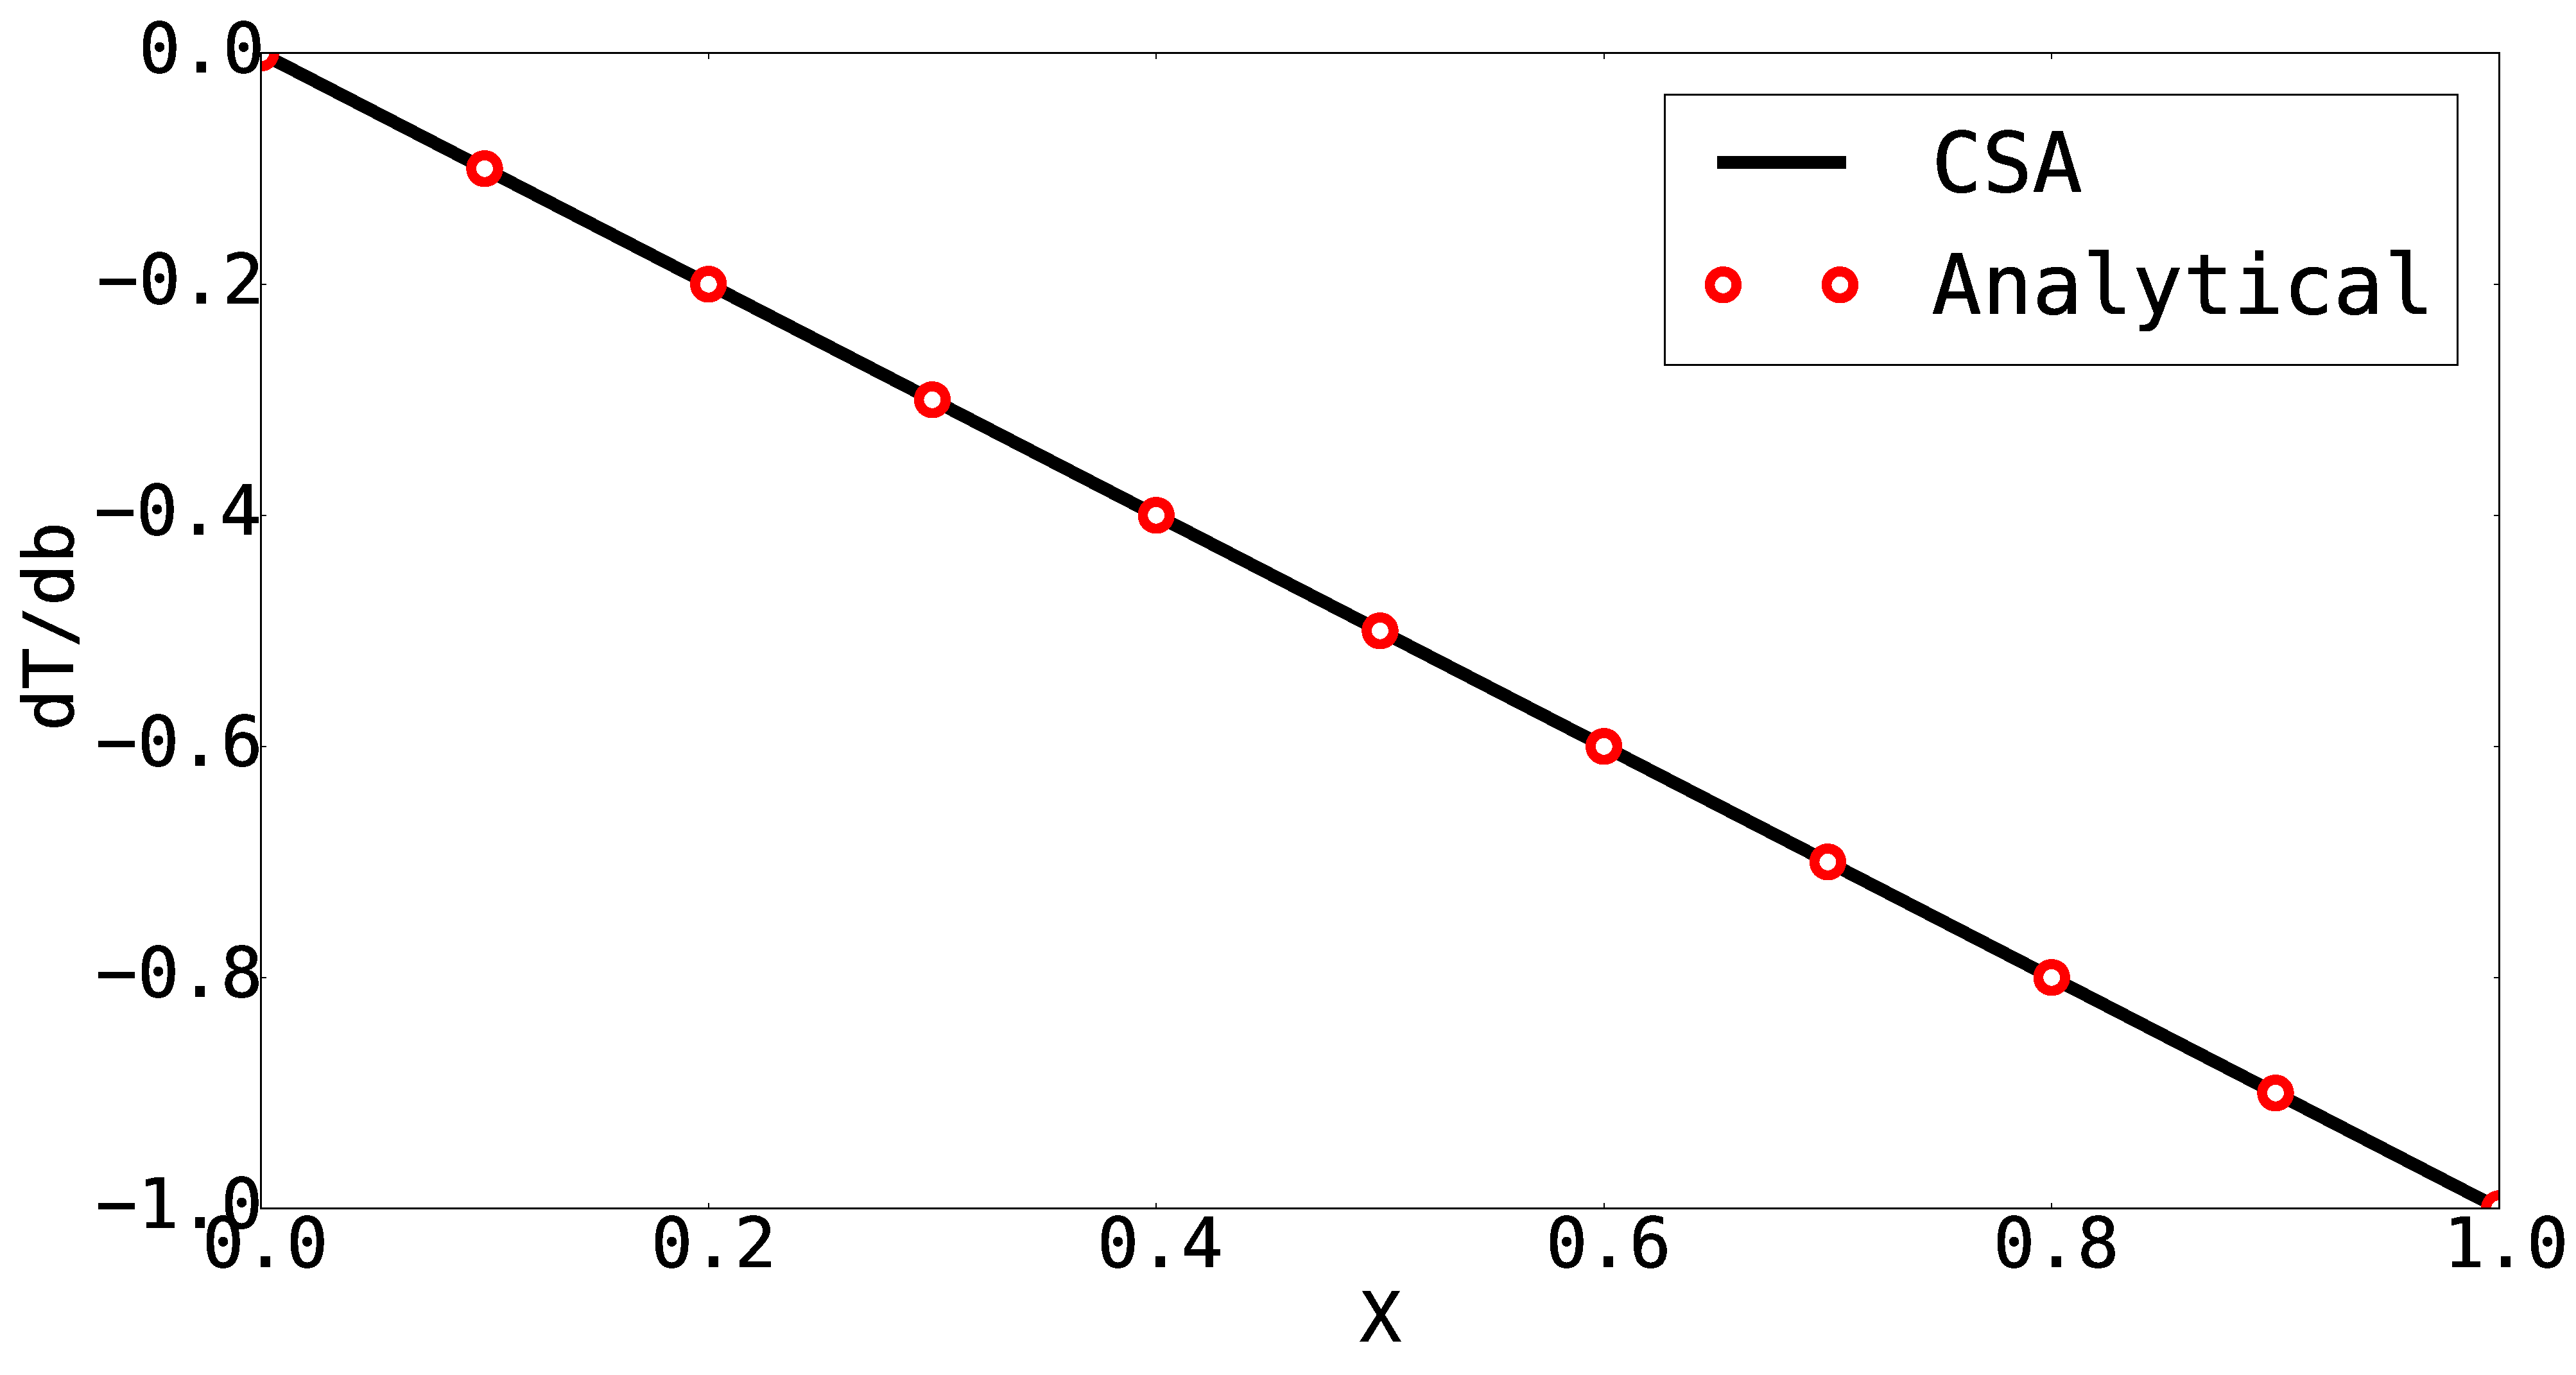
\includegraphics[width=7.0cm]{Chapter_2/figure/CSA_n11.eps}
	}
	\quad
	\subfigure[$n = 41$]
	{
	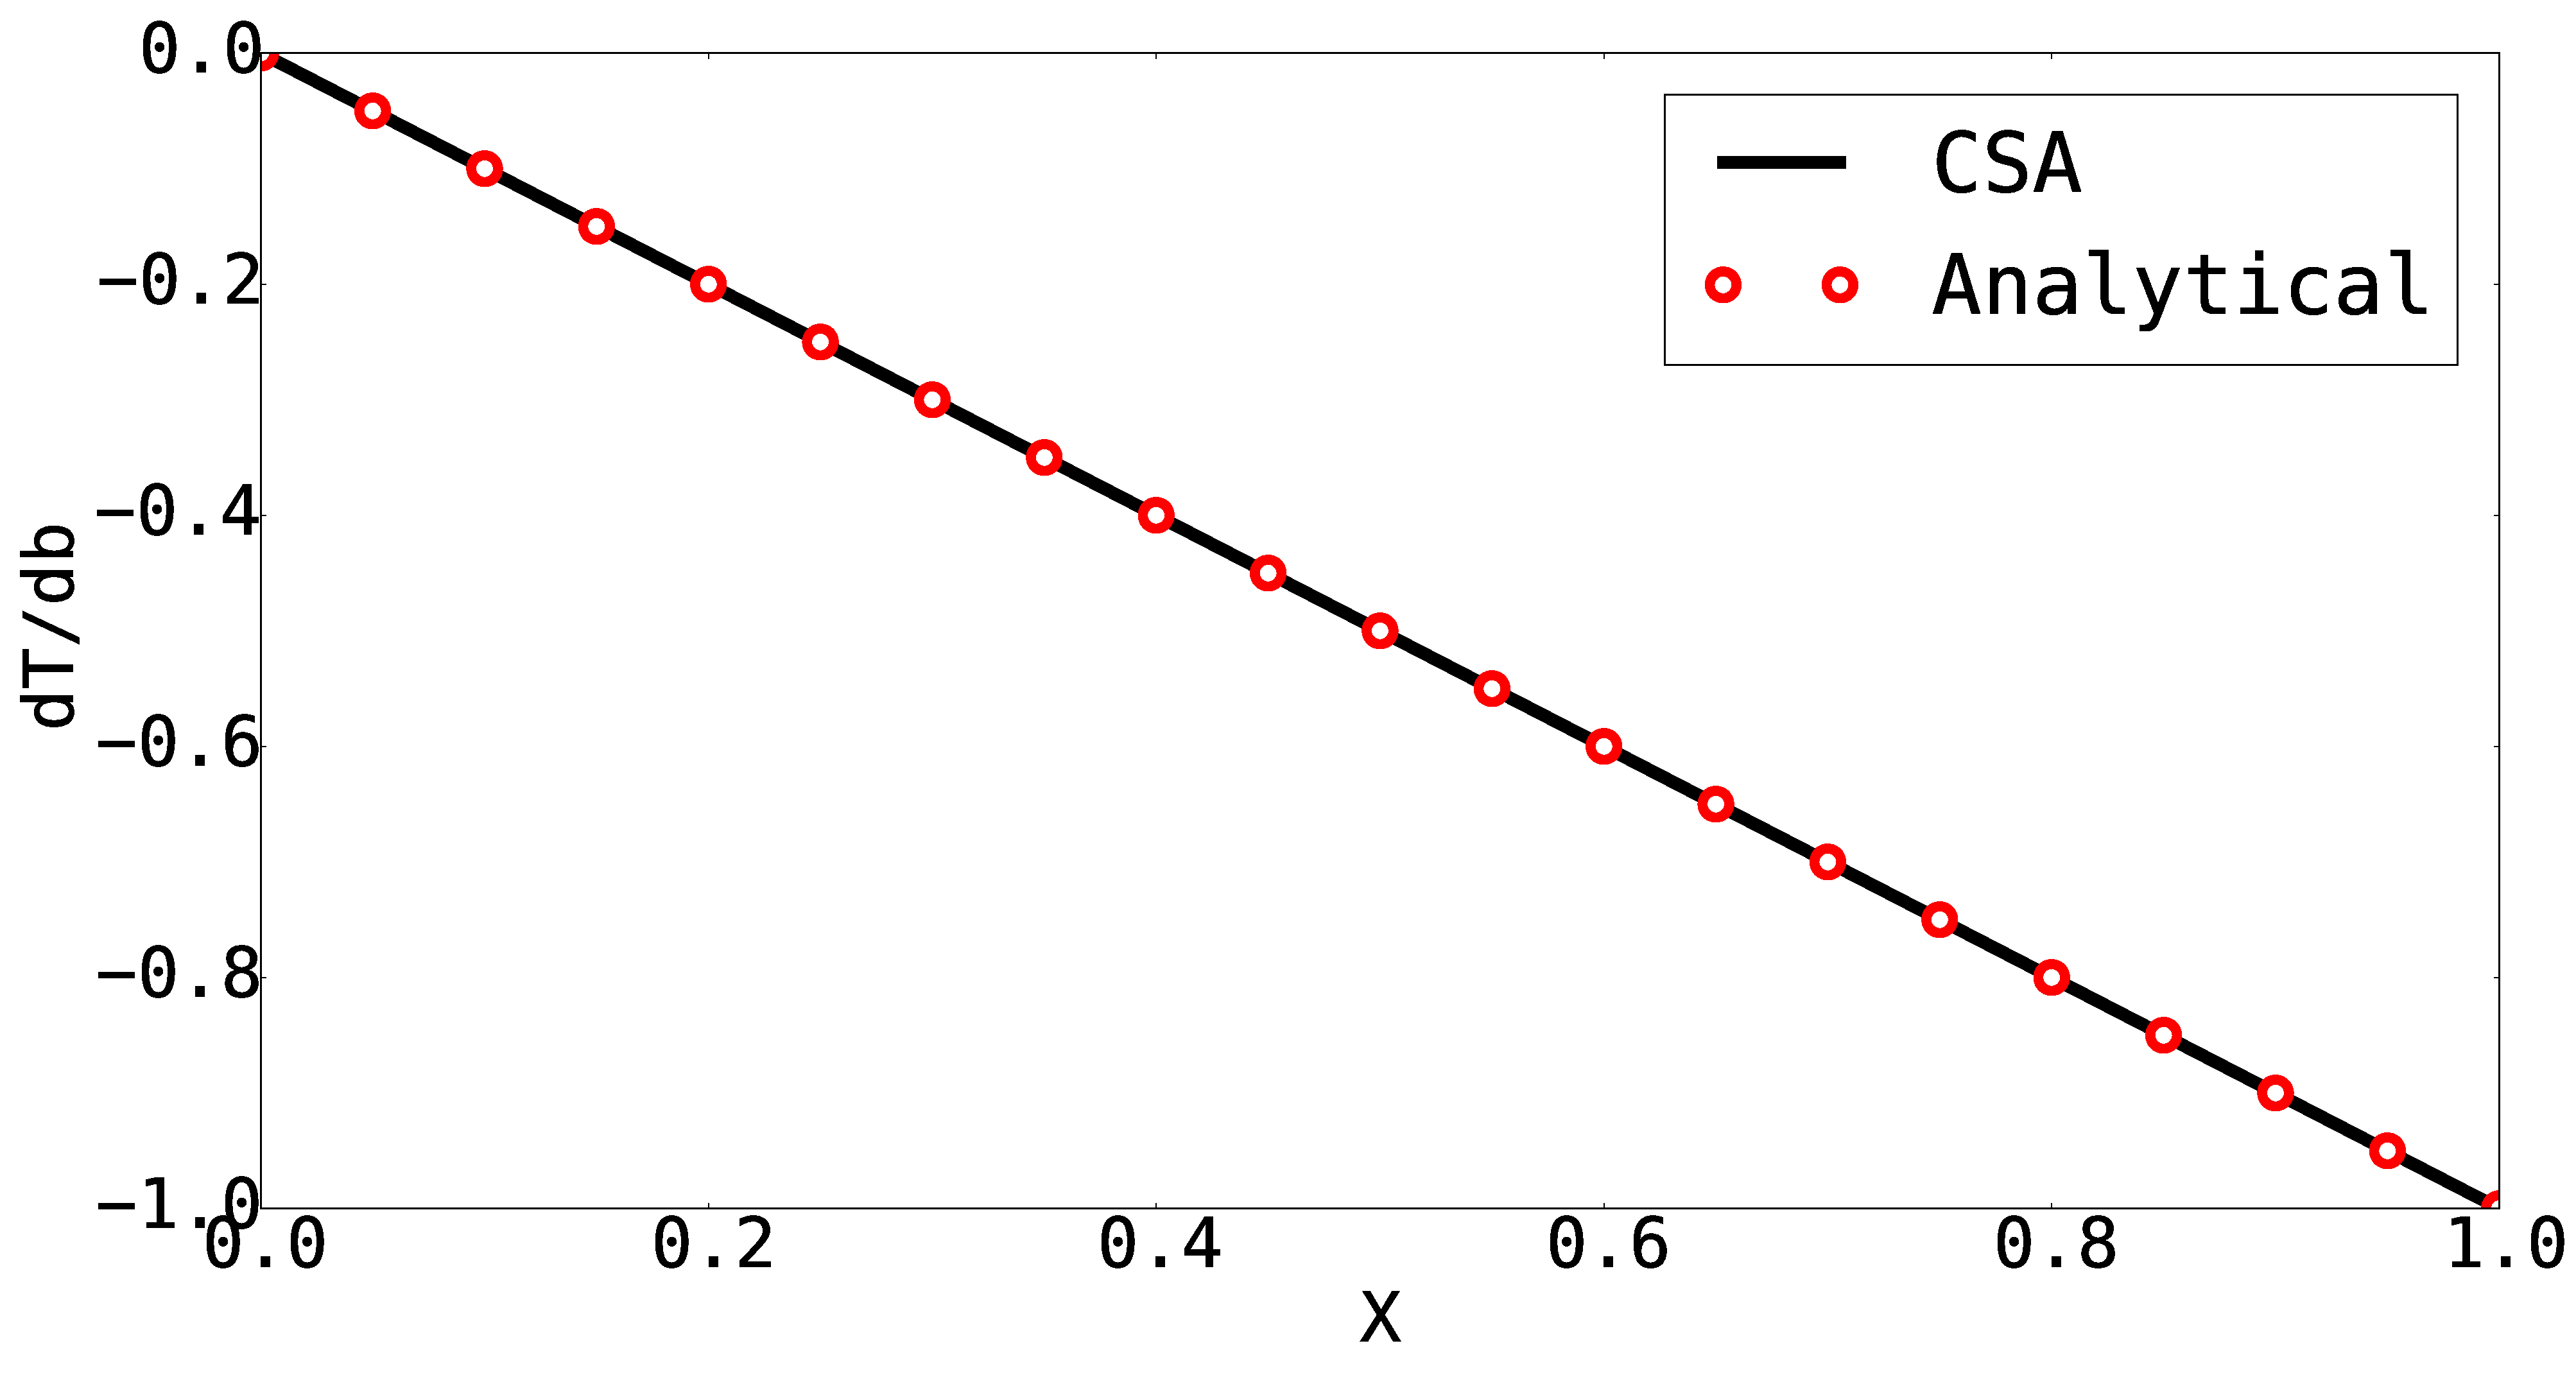
\includegraphics[width=7.0cm]{Chapter_2/figure/CSA_n41.eps}
	}
	\\
	\subfigure[$n = 81$]
	{
	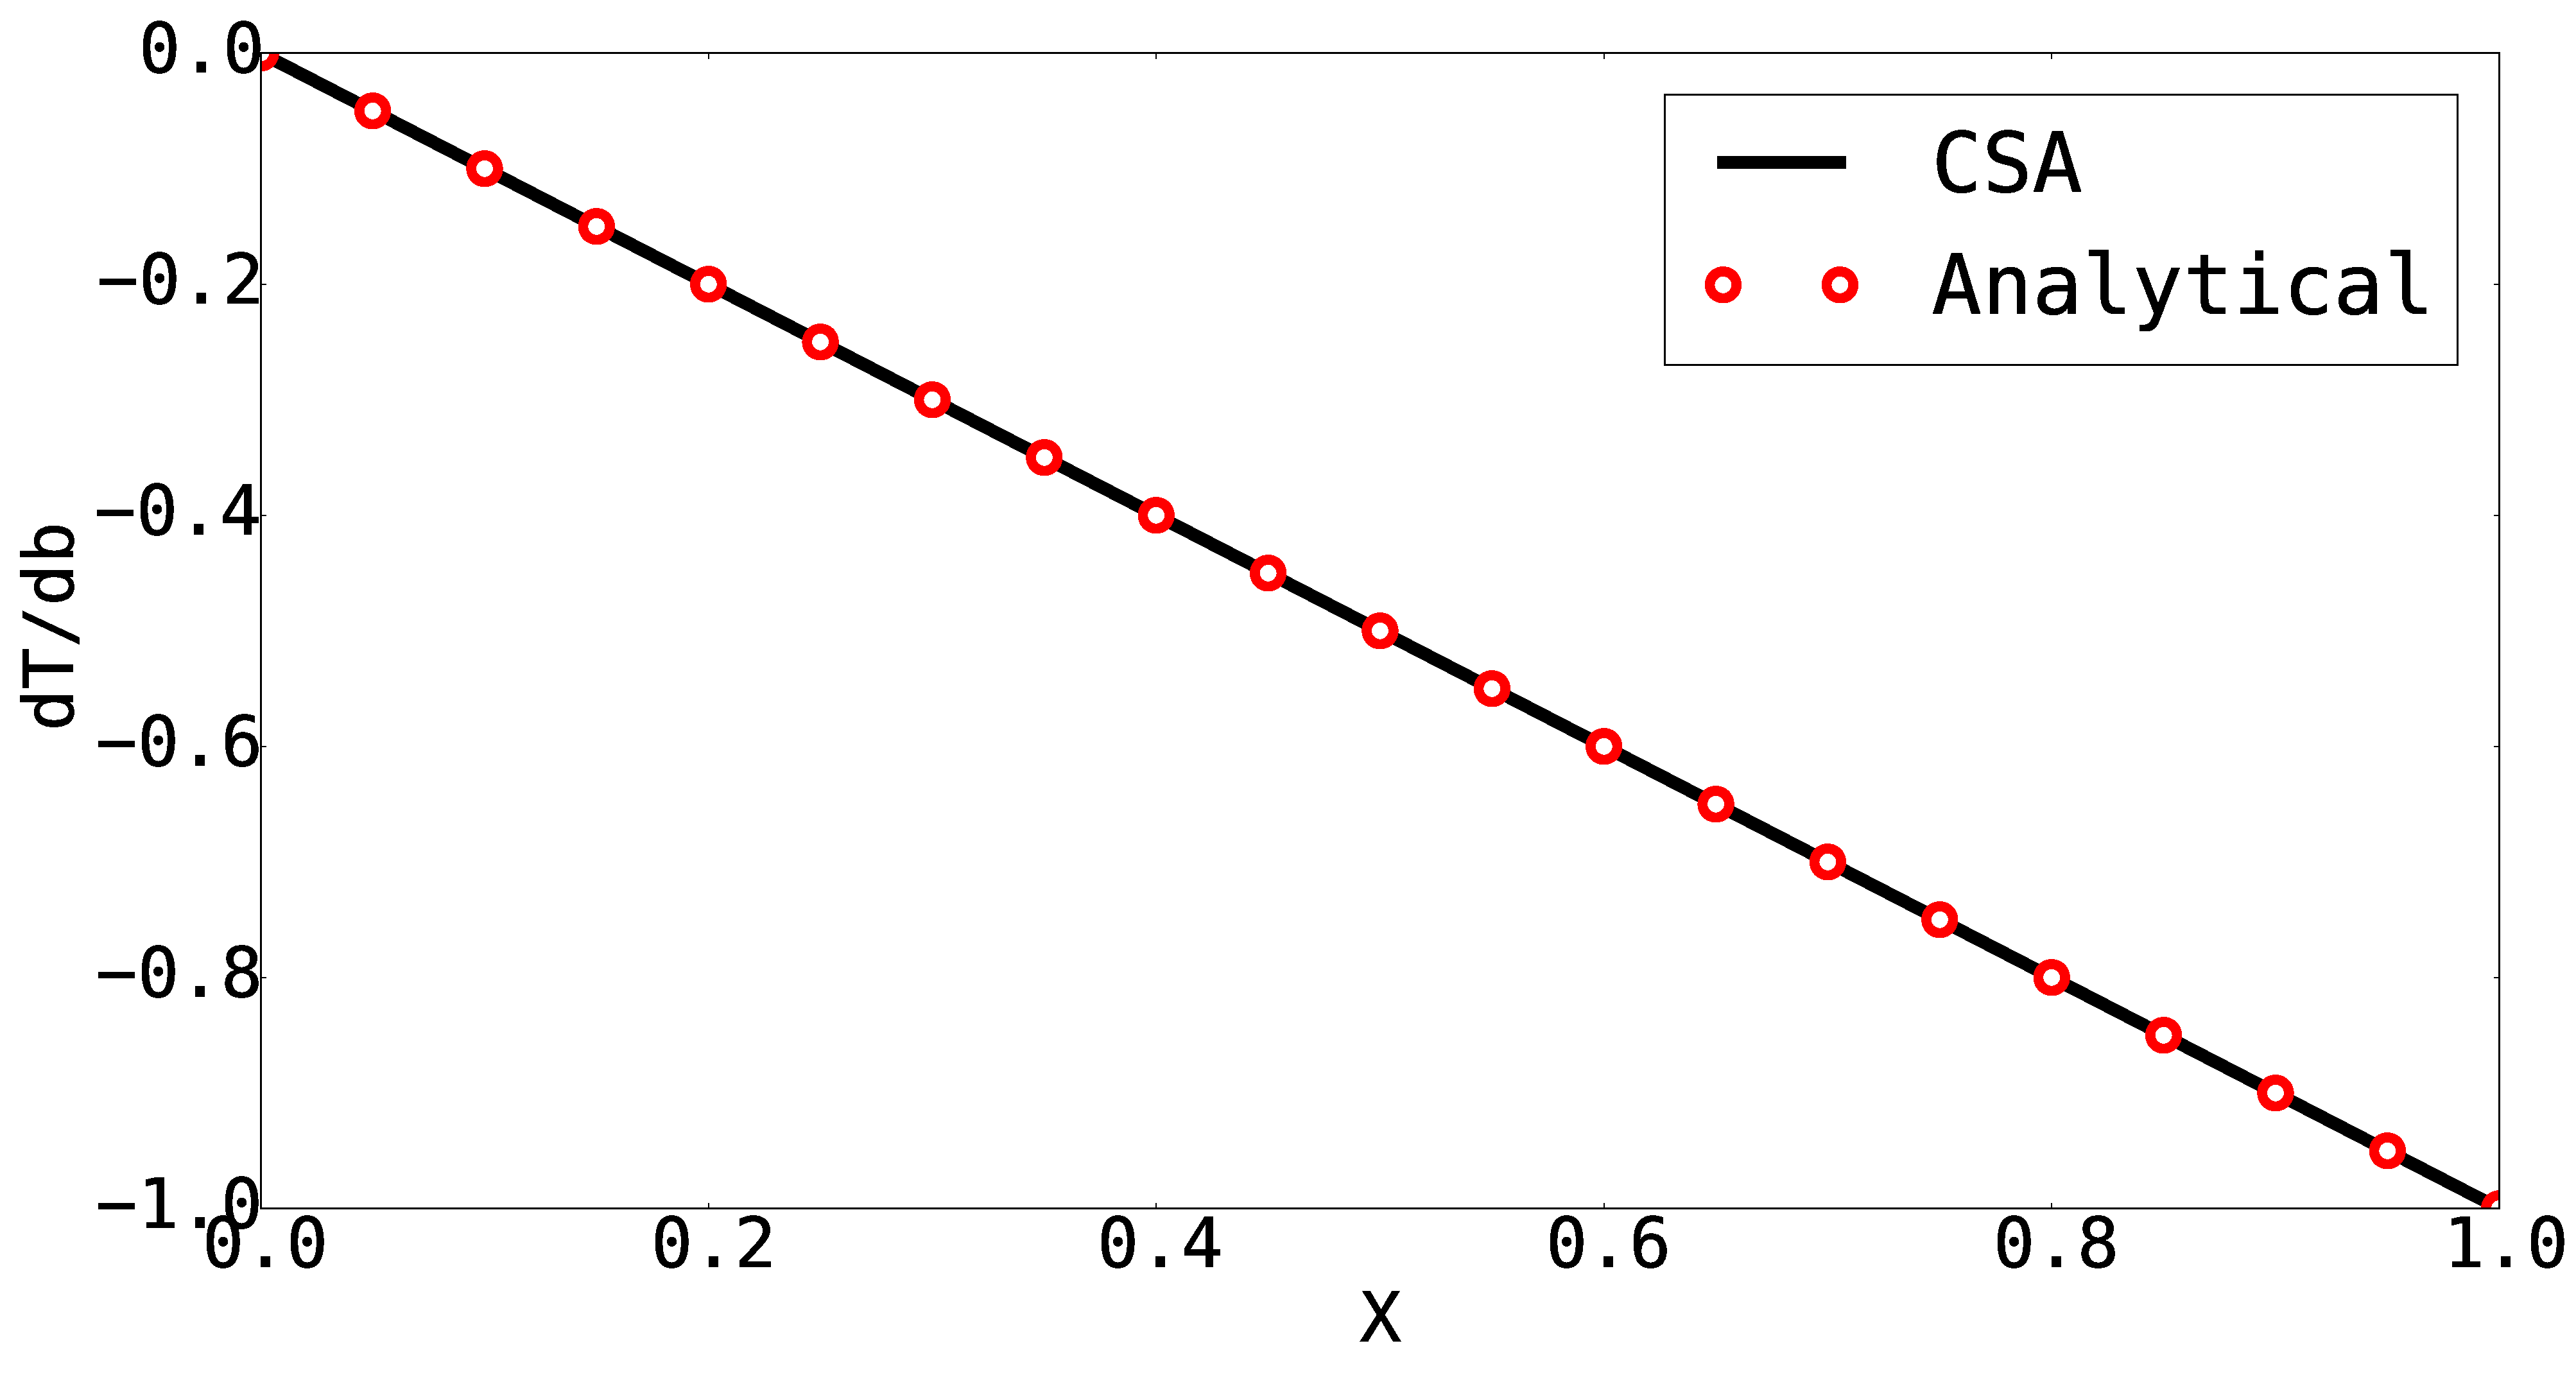
\includegraphics[width=7.0cm]{Chapter_2/figure/CSA_n81.eps}
	}
	\quad
	\subfigure[$n = 161$]
	{
	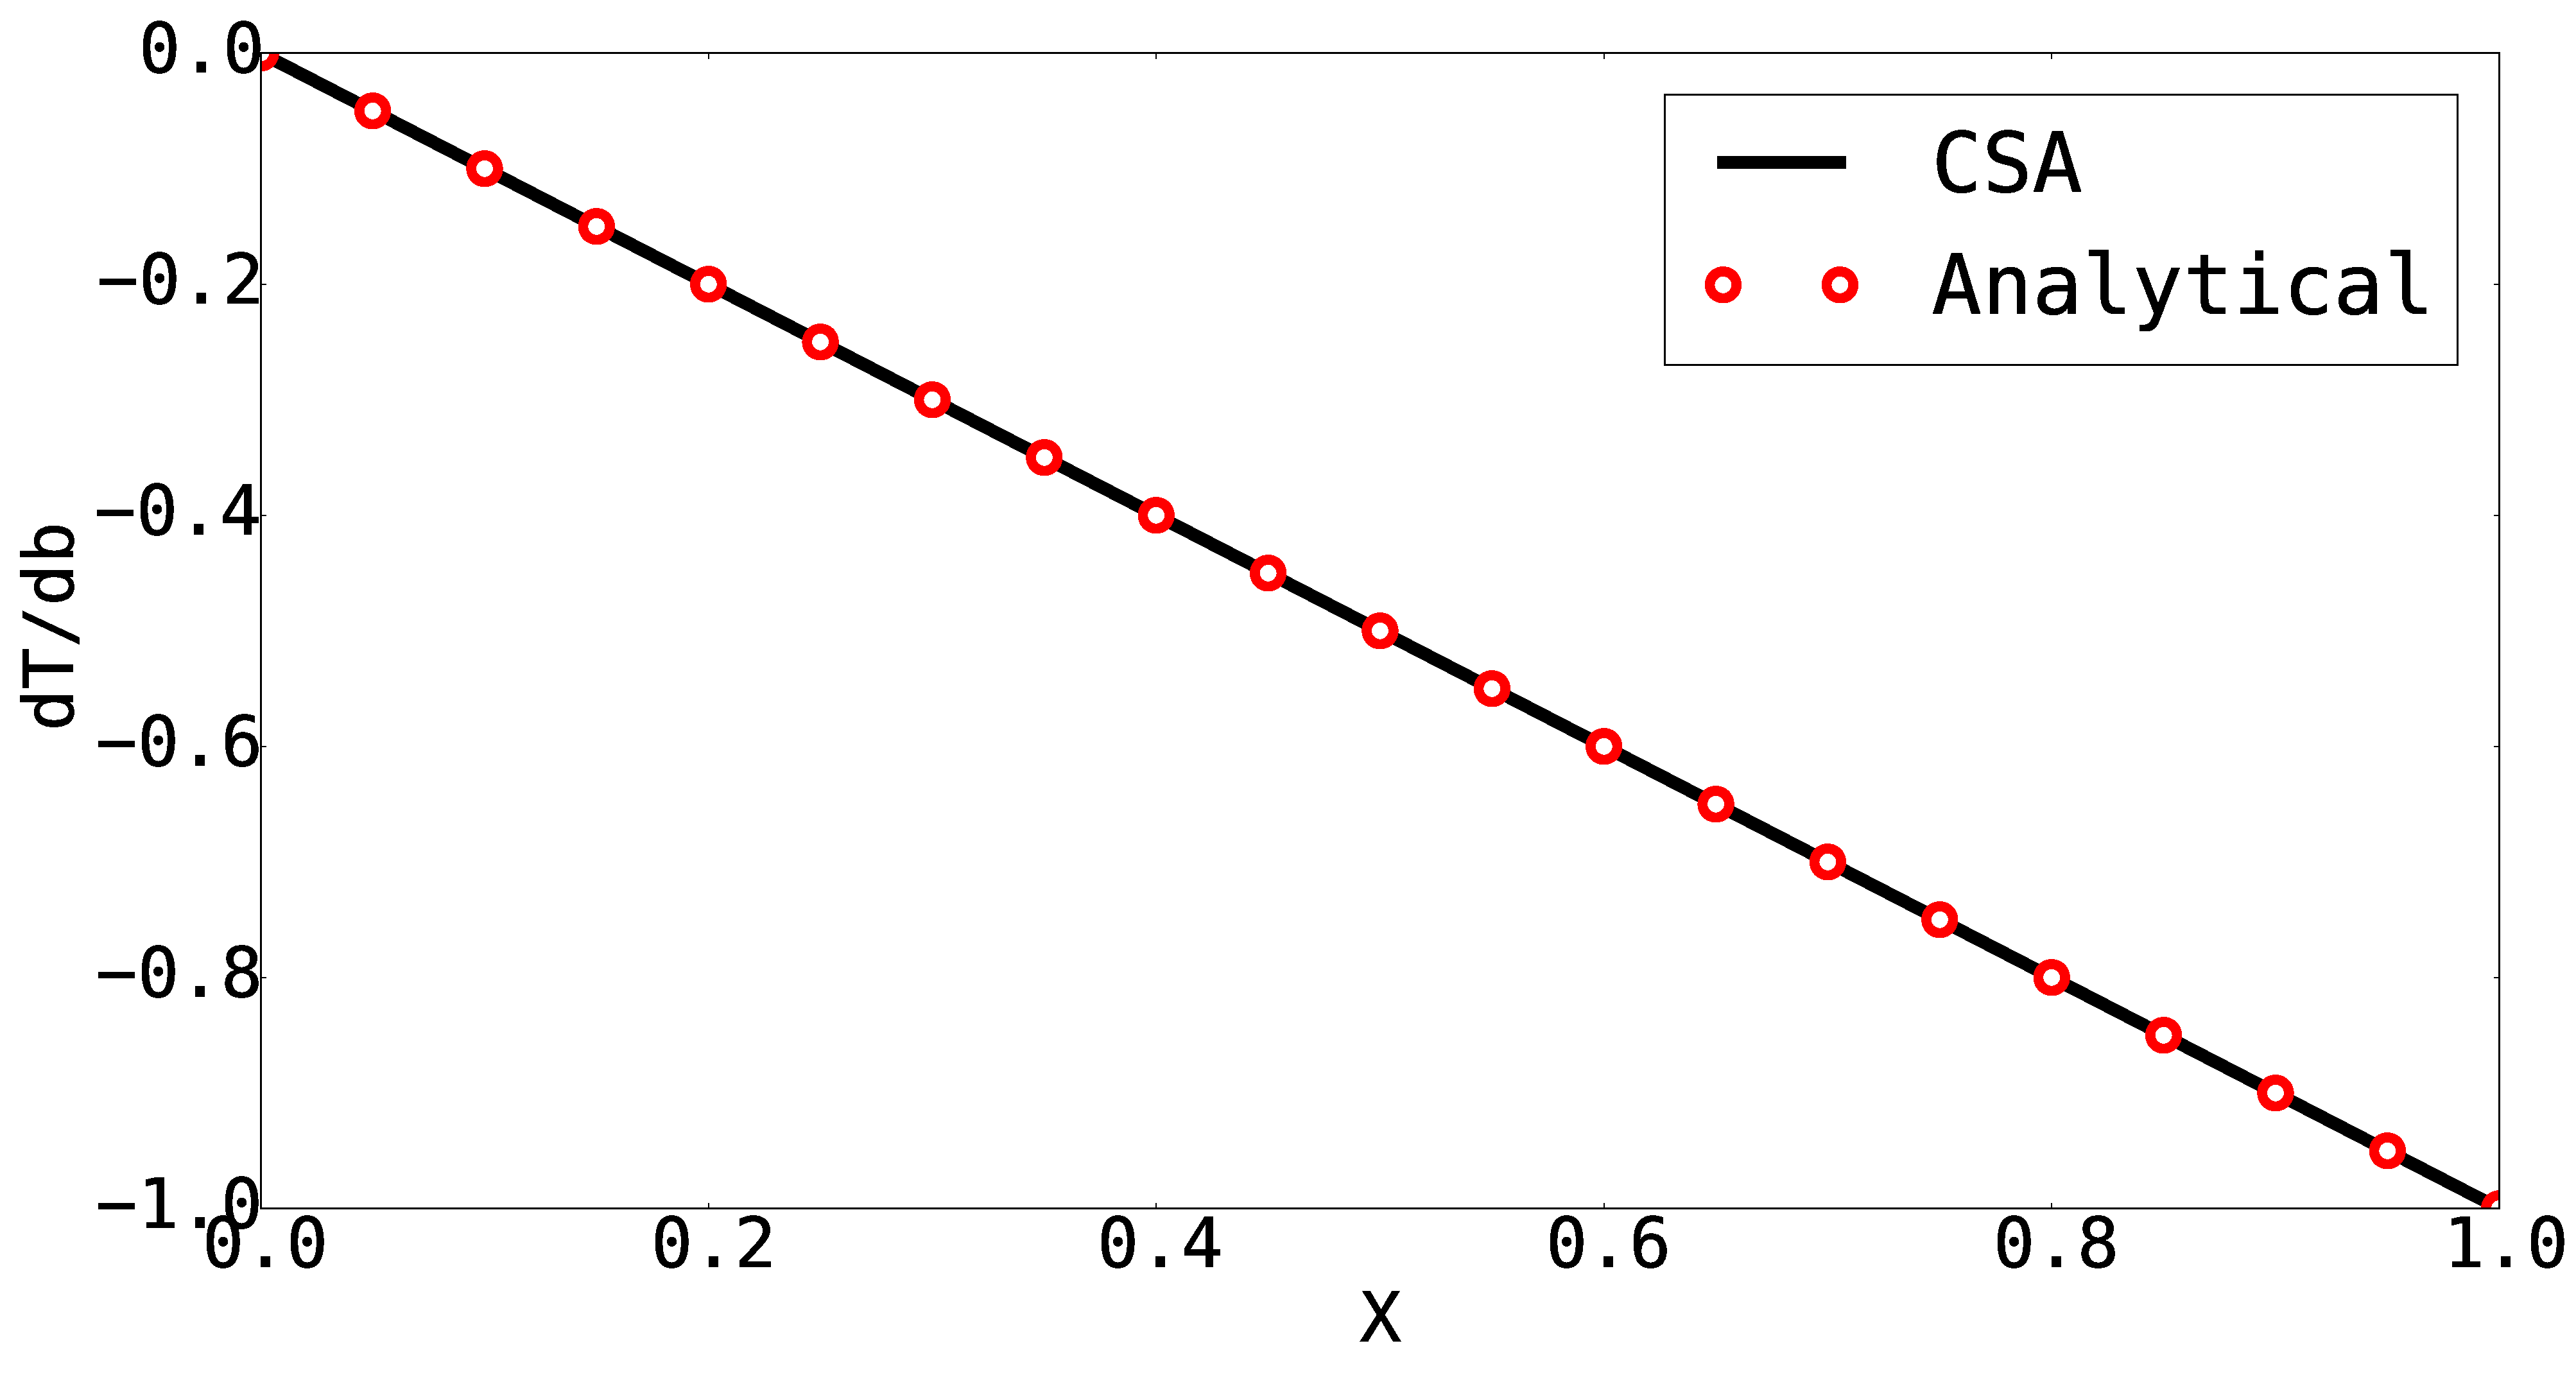
\includegraphics[width=7.0cm]{Chapter_2/figure/CSA_n161.eps}
	}
	\caption{Comparison between continuum sensitivity analysis and analytical results for different number of nodes.}
	\label{fig:C2_comparisonBetweenCSAandAnalytical}
\end{figure}

\begin{table}[H]
\centering
\begin{tabular}{| c | c |}
	\hline
	Number of nodes & NRMSD \\ \hline \hline
	11 & $6.96 \times 10^{-17}$ \\ \hline
	41 & $2.02 \times 10^{-15}$ \\ \hline
	81 & $1.43 \times 10^{-15}$ \\ \hline
	161 & $2.77 \times 10^{-15}$ \\ \hline
\end{tabular}
\caption{RMSE value for different number of nodes.}
\label{table:C2_CSA_NRMSD}
\end{table}

It should be noted that the sensitivity equations are derived and solved in the local form. This does not include the effect of nodes moving in the computational domain. If the analysis requires the sensitivity at the material points, an additional step is required to convert the local sensitivities to their total form using the chain rule as shown in the following equation.

\begin{equation*}
	\frac{DT}{Db} = \frac{\partial T}{\partial b} + \frac{\partial T}{\partial x} \cdot \frac{\partial x}{\partial b}
\end{equation*}

This will add an extra cost to the simulation due to additional step for calculating $\partial x/\partial b$. The reason this step exists is due to movement of computational nodes due to change in shape. Therefore, if the computational nodes can be fixed, the $\partial x/\partial b$ term will be equal to zero. We are proposing to achieve this using a non-body conformal technique such as immersed boundary method. This will be explained in the next chapter in more details.

% ======================================================================================
\section{Summary}
In summary, we looked at two main approaches used to calculate the sensitivity response of a system. The discrete method is based on differentiating the discretized governing equations whereas in continuum method the governing equation are differentiated first and then discretized. We applied these techniques to a simple 1-D heat transfer problem and calculated the sensitivity of response to shape design parameter. The sensitivities are calculated in the local form for each of these methods and compared with the analytical results where they show good comparison. It is showed that by using the continuum sensitivity analysis, the differential operators used in the solution of governing equations are reused in the sensitivity analysis. This effectively means that the black-box solver used in the simulation step can be reused with new boundary conditions for solving the sensitivity response. As showed in the example problem, this is not possible when using discrete method. This is mainly due to the fact that the discrete operators will be affected by differentiating the discretized governing equations with respect to design variables. Therefore, more details about the analysis needs to be known when using discrete approach compared to the continuum. Continuum sensitivity approach is used in this research due to its ability to treat the analysis as black-box for solving both the governing equations and the sensitivity response. However, the result of sensitivity analysis is still the local sensitivities which needs to be transformed to the total form using the chain rule. This is not favourable because it is another step on top of an already expensive analysis. We are proposing to use a non-body conformal approach such as immersed boundary method for analysis to remove this step from the sensitivity calculation.
\chapter{The Immersed Boundary Method}
Immersed boundary methods are class of techniques in computational fluid dynamics where the governing equations are solved on cartesian grid that does not conform to the shape of the body in the flow. This is opposed to well known body-conformal techniques where the computational mesh accurately represents the shape of the domain. The boundary condition on the immersed surfaces are not applied explicitly, instead an extra forcing function is added to the governing equations or the discrete numerical scheme is updated near the boundary. The immersed boundary technique is in special interest to us since it removes the mesh sensitivity calculation from the analysis. In this chapter we talk about different classes of immersed boundary technique and apply them to a simple problem. The applicability of these methods in the continuum sensitivity analysis is also discussed. At the end of this chapter, we will chose couple of immersed boundary techniques for sensitivity analysis implementation.

% ======================================================================================
\section{Introduction}
When people started to use computational models in the design of systems, it was usually sufficient to include single physics into the design. The simulations were usually based on structural solvers using finite elements analysis (FEA) or computational fluid dynamics (CFD) simulations. The design requirements for different systems has been drastically changed compared to the initial designs where these computational methods have been applied. The requirements such as higher fuel efficiency, improved controllability, higher stiffness to mass ratios and lower radar signature have forced the designers to develop more unconventional configurations. For example, on way to reduce the infra-red signature of the aircraft engine is to remove it from hanging underneath the wing and put it inside of the aircraft. However, by doing this as massive heat source will be added the structure. The thermal expansion due to this excessive heat load needs to be incorporated into the structural analysis of the system. It requires a multidisciplinary analysis combining thermal analysis for heat transfer and structural analysis for thermal expansion and other structural loads \cite{deaton2013stiffening}.

The multidisciplinary analysis is required for many engineering application however the one that is used most is the interaction of fluid and a deformable structure. This is commonly known as a Fluid-Solid Interaction (FSI) problem. Fluid–structure interaction (FSI) problems are dealt with in many different engineering applications, such as fluttering and buffeting of bridges \cite{jain1996coupled}, vibration of wind turbine blades \cite{arrigan2011control}, aeroelastic response of airplanes \cite{farhat2006provably}. FSI problems are also seen in blood flows in arteries and artificial heart valves \cite{sotiropoulos2009review}, flying and swimming \cite{kern2006simulations}. The conventional approach for simulating such problems is the Arbitrary Lagrangian–Eulerian (ALE) method. ALE methods are based on body- conforming grids to track the location of the fluid–structure interface. ALE methods have been applied to many FSI problems however, they are cumbersome if not impossible to apply to FSI problems with large deformations for complicated boundary shapes.

Immersed boundary (IB) methods are considered a separate family of methods used for modelling FSI problems with complicated boundary shapes and large deformations. IB methods, are based on solving the governing equations for fluids on a fixed grid. Although this computational grid can be structured (Cartesian) or unstructured, most methods are based on structured grid. When using structured grid, extremely efficient computational methods can be utilized on to solve the governing equations. The fluid–structure boundaries are represented by a set of independent nodes. The solid boundary effect on the flow is formulated either by introducing fictitious body forces in the governing equations or by locally modifying the structure of the background grid.

IB has several advantages over the ALE methods. Probably the biggest advantage is the simplification of the task of grid generation. Generating body-conformal grid for a complex shape is usually very complicated. The objective is to construct a grid that provides adequate local resolution with the minimum number of total grid points.  This requires a significant input from the user and is an iterative process. For complicated boundaries the unstructured grid approach is better suited however the grid quality is reduced for extremely complicated geometry. In contrast, for a simulation carried using an IB method, grid complexity and quality are not affected by the complexity of the geometry. 

This advantage becomes even more clear for flows with moving boundaries. The ALE approach requires generating a new mesh or deforming the old mesh to match the new boundary shape at each time step. The solution from last time step is also required to be projected to this new computational mesh. Both of the deformation/projection can affect the accuracy, robustness and the computational cost associated the the simulation. On the other hand, the boundary motion in IB method can be handled with rather ease because the computational mesh does not depend on the shape of the boundary. Therefore, although a significant progress in simulating flows using ALE methods has been made in the recent years \cite{lomtev1999discontinuous, farhat2004cfd, cheng2005fluid}, the IB method still remains an attractive alternative for such problems due to its simplicity and cost.

In the following sections of this chapter we first look at the governing equations for the fluid and solid domain. Followed by this different approaches for modelling the follow using IB method are discussed in detail. We apply different IB techniques to a simplified problem to compare the efficiency and simplicity of implimentation. The results are compared with body-conformal solution approach for accuracy comparison. Finally we assess different IB methods with regards to their applicability of the Continuum Sensitivity Analysis (CSA) framework.

% ======================================================================================
\section{Governing Equations}
In the fluid region $\Omega_f$, the governing equations for incompressible flow of a Newtonian fluid are known as Navier-Stokes (NS) equations. In the compact indicial notation, the NS equations are written as

\begin{subequations}\label{eq:C3_GE}
\begin{equation}\label{eq:C3_continuity}
	\frac{\partial u_i}{\partial x_i} = 0
\end{equation}
\begin{equation}\label{eq:C3_momentum}
	\frac{\partial u_i}{\partial t} + \frac{\partial u_i u_j}{\partial x_j} = 
	-\frac{1}{\rho_f	} \frac{\partial p}{\partial x_i} + 
	\nu \frac{\partial}{\partial x_j} \left( \frac{\partial u_i}{\partial x_j} \right) + 
	f_i
\end{equation}
\end{subequations}

where the repeated indices imply summation and $i,j=1,2,3$. $x_i$ are the spatial coordinates, $u_i$ are the velocity components of the fluid in $i$ direction, $\rho_f$ is the fluids density, $p$ is the pressure, $\nu$ is the kinematic viscosity, and $f_i$ are body forces. These forces are used in the IB technique to represent the effect of immersed boundaries on the fluid. In general purpose CFD solvers, due to the use of unstructured grid to represent the shape, it is usually required to use mappings (Jacobian) to convert the physical coordinate the a computational coordinate. This will become problematic when we have skewed elements with cause the mapping become singular. This step is removed in the IB approach since the governing equations \eqref{eq:C3_GE} are discretized on a Cartesian  grid.

The solid domain is modelled using linear elastic theory in this work. The governing equations are written as

\begin{subequations}\label{eq:C3_linearEalsticityEquations}
\begin{equation}
	\sigma_{ji,j} + F_i = \rho_s \partial_{tt} u_i
\end{equation}
\begin{equation}
	\epsilon_{ij} = \frac{1}{2} \left( u_{j,i} + u_{i,j} \right)
\end{equation}
\begin{equation}
	\sigma_{ij} = C_{ijkl} \epsilon_{kl}
\end{equation}
\end{subequations}

where $\sigma$ is the Cauchy stress tensor, $\epsilon$ is the strain tensor, $u$ is the displacement vector, $C$ is stiffness tensor, $F$ is the body force, and $\rho_s$ is the mass density of solid. These governing equations are solved to track the motion of of the solid boundary. 

To solve the coupled system of equations of \eqref{eq:C3_GE} and \eqref{eq:C3_linearEalsticityEquations} we need to have boundary conditions. The boundary conditions of \eqref{eq:C3_GE} are defined as pressure or velocity magnitudes on the outer boundaries of the domain. After solving Equation \eqref{eq:C3_GE}, the loads on the structure can be calculated by integrating the pressure from the fluid solid over the solid boundaries. This will be the boundary load used for solving Equation \eqref{eq:C3_linearEalsticityEquations}. When the governing equation for the solid region is solved, the displacement of the solid domain is known. This is fed into the CFD solver to update the solid boundary location for fluid domain. This will change the solution of fluid's solver resulting in different pressure distribution. This process is repeated until a convergence is satisfied. The convergence can be defined as change in the structure deflection for two subsequent steps for a static problem.

% ======================================================================================
\section{Benchmark Case}\label{sec:C3_benchmark_case}
We define a 1D benchmark problem to investigate different IB formulations in detail. In one dimensional space the equations of incompressible flow are not very interesting and it is not simple to write a one-dimensional analogue of the IB to capture all of its features. However, for a simple one dimensional problem we can understand different formulations of IB method and later apply it to higher dimensions. Moreover, for the sake of sensitivity analysis better understanding of the problem can be achieved for a simplified model. The other reason for working with a simplified model is the availability of analytical results that can be used for verifying the results we get from the numerical solvers. As the final note, for this benchmark case we mainly focused on the fluid domain, the structures can be easily added to this formulation.

To derive the one dimensional benchmark case we start with the Navier-Stokes equations. Consider a viscous incompressible fluid in the channel $0 \geq y \leq 1$, $-\infty < x < \infty$ as shown in Figure \ref{fig:C3_benchmarkCase}.

\begin{figure}[H]
	\centering
	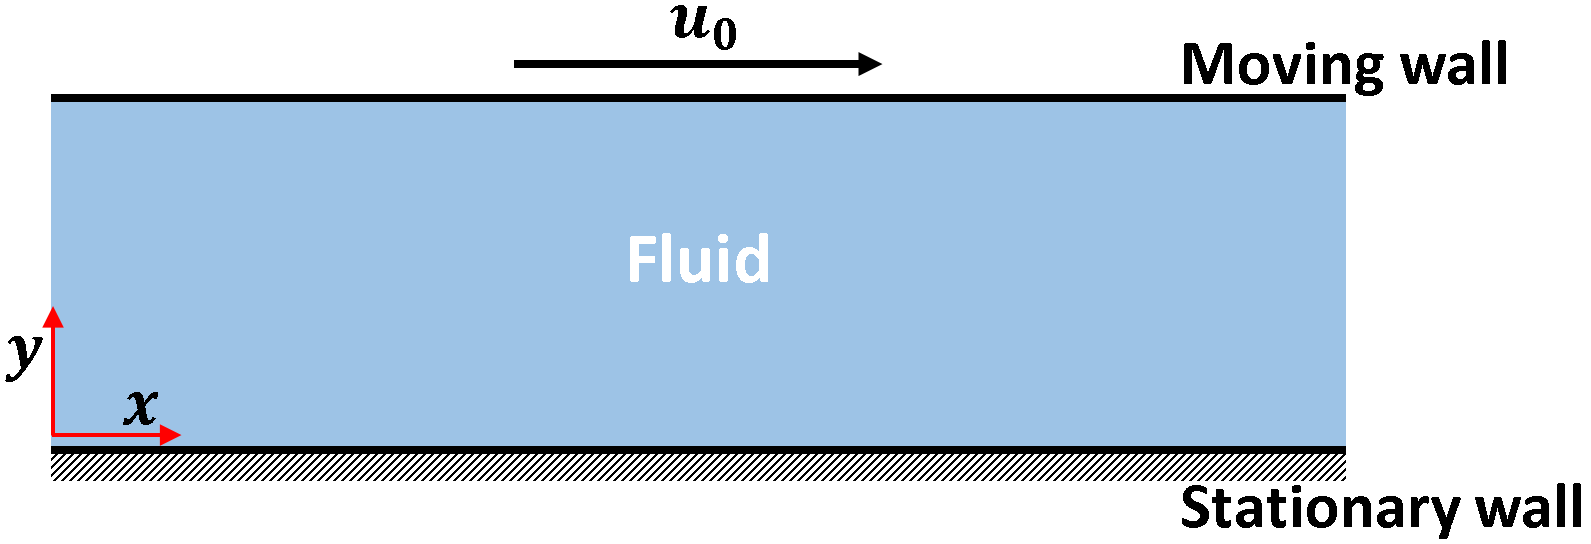
\includegraphics[width=14.00cm]{Chapter_3/figure/C3_infinite_channel.png}
	\caption{1D benchmark case for IB method.}
	\label{fig:C3_benchmarkCase}
\end{figure}

We can also assume that the boundary conditions are periodic in $x$. Next suppose that there is a horizontal plate running through the length of this channel at $y=y_0$ and moving with $u_0$ velocity in horizontal direction. We assume no-slip condition where the fluid and the plate meet. This will force the fluid to accelerate in $x$ direction due to the viscous stress from the moving plate. We expect no motion in $y$ direction and can drop all terms in the NS equations containing $u_j$ velocity. Due to the continuity equation \eqref{eq:C3_continuity}, there is no variation in the $x$ direction so we can drop all the terms that involve with $x$ variation as well. This enables us to simplify the NS equation of \eqref{eq:C3_momentum} into Equation \eqref{eq:C3_benchmarkProblem}. It should be noted that the continuum equation \eqref{eq:C3_continuity} is automatically satisfied.

\begin{subequations}\label{eq:C3_benchmarkProblem}
\begin{equation}
	u_t = \mu u_{yy} \quad \text{in } \Omega_f
\end{equation}
\begin{equation}
\begin{cases}
	u = u_0 \quad \text{at } y = 1 \\
	u = 0 \quad \text{at } y = 0
\end{cases}
\end{equation}
\end{subequations}

Equation \eqref{eq:C3_benchmarkProblem} is transient in nature however, its steady state solution can be calculated by setting the time derivative equal to zero. This equation governs what is commonly known as Couette flow in introductory courses in fluid dynamics. The analytical solution for this equation is shown in Equation \eqref{eq:C3_benchmarkAnalyticalSolution}.

\begin{equation}\label{eq:C3_benchmarkAnalyticalSolution}
	u = u_0 x
\end{equation}

We will use this analytical solution to verify the result of the different IB methods defined in the following sections.

% ======================================================================================
\section{Immersed Boundary Classification}
In general, IB methods can be classified in three main families: i) discrete forcing, ii) continuum forcing, and iii) cut-cell methods. This classification is based on how the interface conditions are handled in the IB algorithm. In this section we present the essence of each method and try to point their primary advantages and disadvantages. Moreover, each of the discussed IB techniques will be applied to the benchmark problem where the results are verified with the analytical solution. In general, the immersed boundary approach is based on modifying the NS equations for imposing the boundary conditions. This modification can be done in three different ways that leads to a fundamental dichotomy in IB method.

% ======================================================================================
\section{Discrete Forcing Method}
\subsection{Formulation}
\subsection{Implimentation for Couette Flow Problem}

% ======================================================================================
\section{Continuum Forcing Method}
In this implementation of the immersed boundary, a forcing equation is added to the continuous governing equation \eqref{eq:C3_momentum} to represent the effect of the boundary. The continuous IB technique is the original method developed by Peskin \cite{peskin1972flow} for coupled simulation of blood flow due to the contraction of heart muscle. In this approach, the immersed boundary is represented by a set of elastic fibers that their locations are tracked in a Lagrangian fashion by a collection of massless points. These points move with the local fluid velocity. Therefore, the location of the $k$-th Lagrangian point, $X_k$ is governed by the following equation

\begin{equation}
	\frac{\partial X_k}{\partial t} = u(X_k, t)
\end{equation}

where $u$ is the velocity of the fluid at location $X_k$. The location of fluid nodes, $x$, does not necessary coincide with the location of the Lagrangian points. Thus, it is required to map the velocities from the Eulerian domain, where the fluid's equation of motion are solved, to Lagrangian nodes. In a purely continuum problem, this can be done using the Dirac delta functions. The property of the Dirac delta function that enables the mapping between the Euler and Lagrangian domain is shown in the following equation

\begin{equation}
	\int_{\Omega_f} f(x) \delta(x - X_k) = f(X_k)
\end{equation}

As can be seen here, by convoluting the function of interest and the delta function, we can evaluate our function of interest at any location where the delta function is defined. By defining the delta function at $X_k$ and using velocity from CFD solver as function $f$, we can evaluate the needed velocity for IB at any arbitrary point $X_k$. Although this is the main idea of mapping data to Lagrangian domain, this approach becomes unstable in practice \cite{lee2003stability}. In the practical implementation of immersed boundary method, the effect of delta function need to be expanded to couple of nodes around $X_k$. This is achieved by relaxing the delta function. The relaxed delta function is generally refereed to as regularized delta function \cite{shin2008assessment}. The regularized delta function is defined using Equation \eqref{eq:C3_regularizedDeltaFunction} in three dimensions.

\begin{equation}\label{eq:C3_regularizedDeltaFunction}
	\delta_h(x_1, x_2, x_3) = \frac{1}{dx_1 \cdot dx_2 \cdot dx_3}
							   \phi \left( \frac{x_1 - \eta_1}{dx_1} \right)
							   \phi \left( \frac{x_2 - \eta_2}{dx_2} \right)
							   \phi \left( \frac{x_2 - \eta_3}{dx_3} \right)
\end{equation}

where $x_i$ is the spatial coordinate in each direction, $\eta_i$ is the location where the delta function is defined, and $dx_i$ is the grid size in each direction. In above equation $i$ can be $1$, $2$, or $3$. The $\phi$ function is defined in Equation \eqref{eq:C3_phiFunction}. As shown here there are different ways of defining this function. The input of $\phi$ function is $r$ which is defined as $(x_i - \eta_i) / dx_i$.

\begin{subequations}\label{eq:C3_phiFunction}
\begin{equation}\label{eq:C3_phiFunction_2point}
	\phi(r) = 
	\begin{cases}
	1 - |r| \quad &|r| \leq 1 \\
	0	\quad &\text{otherwise}
	\end{cases}
\end{equation}
\begin{equation}\label{eq:C3_phiFunction_3point}
	\phi(r) = 
	\begin{cases}
		\frac{1}{3} \left( 1 + \sqrt{-3r^2 + 1} \right) \quad &|r| \leq 0.5 \\
		\frac{1}{6} \left( 5 - 3|r| - \sqrt{-3(1 - |r|)^2 + 1} \right) & 0.5 \geq |r| \leq 1.5 \\
		0 & \text{otherwise}
	\end{cases}
\end{equation}
\begin{equation}\label{eq:C3_phiFunction_4point}
	\phi(r) = 
	\begin{cases}
		\frac{1}{8}
		\left(
		3 - 2|r| + \sqrt{1 + 4|r| - 4r^2}
		\right) \quad &0 \leq |r| \leq 1
		\\
		\frac{1}{8}
		\left(
		5 - 2|r| + \sqrt{-7 + 12|r| - 4r^2}
		\right) \quad &1 \leq |r| \leq 2
		\\
		0 &\text{otherwise}
	\end{cases}
\end{equation}
\begin{equation}\label{eq:C3_phiFunction_6point}
	\phi(r) = 
	\begin{cases}
		\begin{split}
		\frac{61}{112} - \frac{11}{42} |r| - \frac{11}{56} |r|^2 + \frac{1}{12} |r|^3 + 
		\frac{\sqrt{3}}{336}
		\left( 243 + 1584 |r| \right. \\
		\left. - 748 |r|^2 - 1560 |r|^3 + 500 |r|^4 + 336 |r|^5 - 112 |r|^6
		\right)^{1/2}
		\end{split} \quad & 0 \leq |r| \leq 1
		\\
		\frac{21}{16} + \frac{7}{12} |r| - \frac{7}{8} |r|^2 + \frac{1}{6} |r|^3 - 
		\frac{3}{2} \phi \left( |r| - 1 \right) & 1 \leq |r| \leq 2
		\\
		\frac{9}{8} - \frac{23}{12} |r| + \frac{3}{4} |r|^2 - \frac{1}{12} |r|^3 + 
		\frac{1}{2} \phi \left( |r| - 2 \right) & 2 \leq |r| \leq 3
		\\
		0 & \text{otherwise}
	\end{cases}
\end{equation}
\end{subequations}

Equation \eqref{eq:C3_phiFunction_2point} is the 2-point delta function that does the linear interpolation between the points point \cite{saiki1996numerical}. Equation \eqref{eq:C3_phiFunction_3point} shoes the 3-point delta function used by Roma et al. \cite{roma1999adaptive}, and Equation \eqref{eq:C3_phiFunction_4point} and \eqref{eq:C3_phiFunction_6point} are 4-point and 6-point delta functions used by Peskin \cite{peskin2002immersed}. The comparison between the shape of different $\phi(r)$ functions are shown in Figure \ref{fig:C3_phi_function}

\begin{figure}
	\centering
	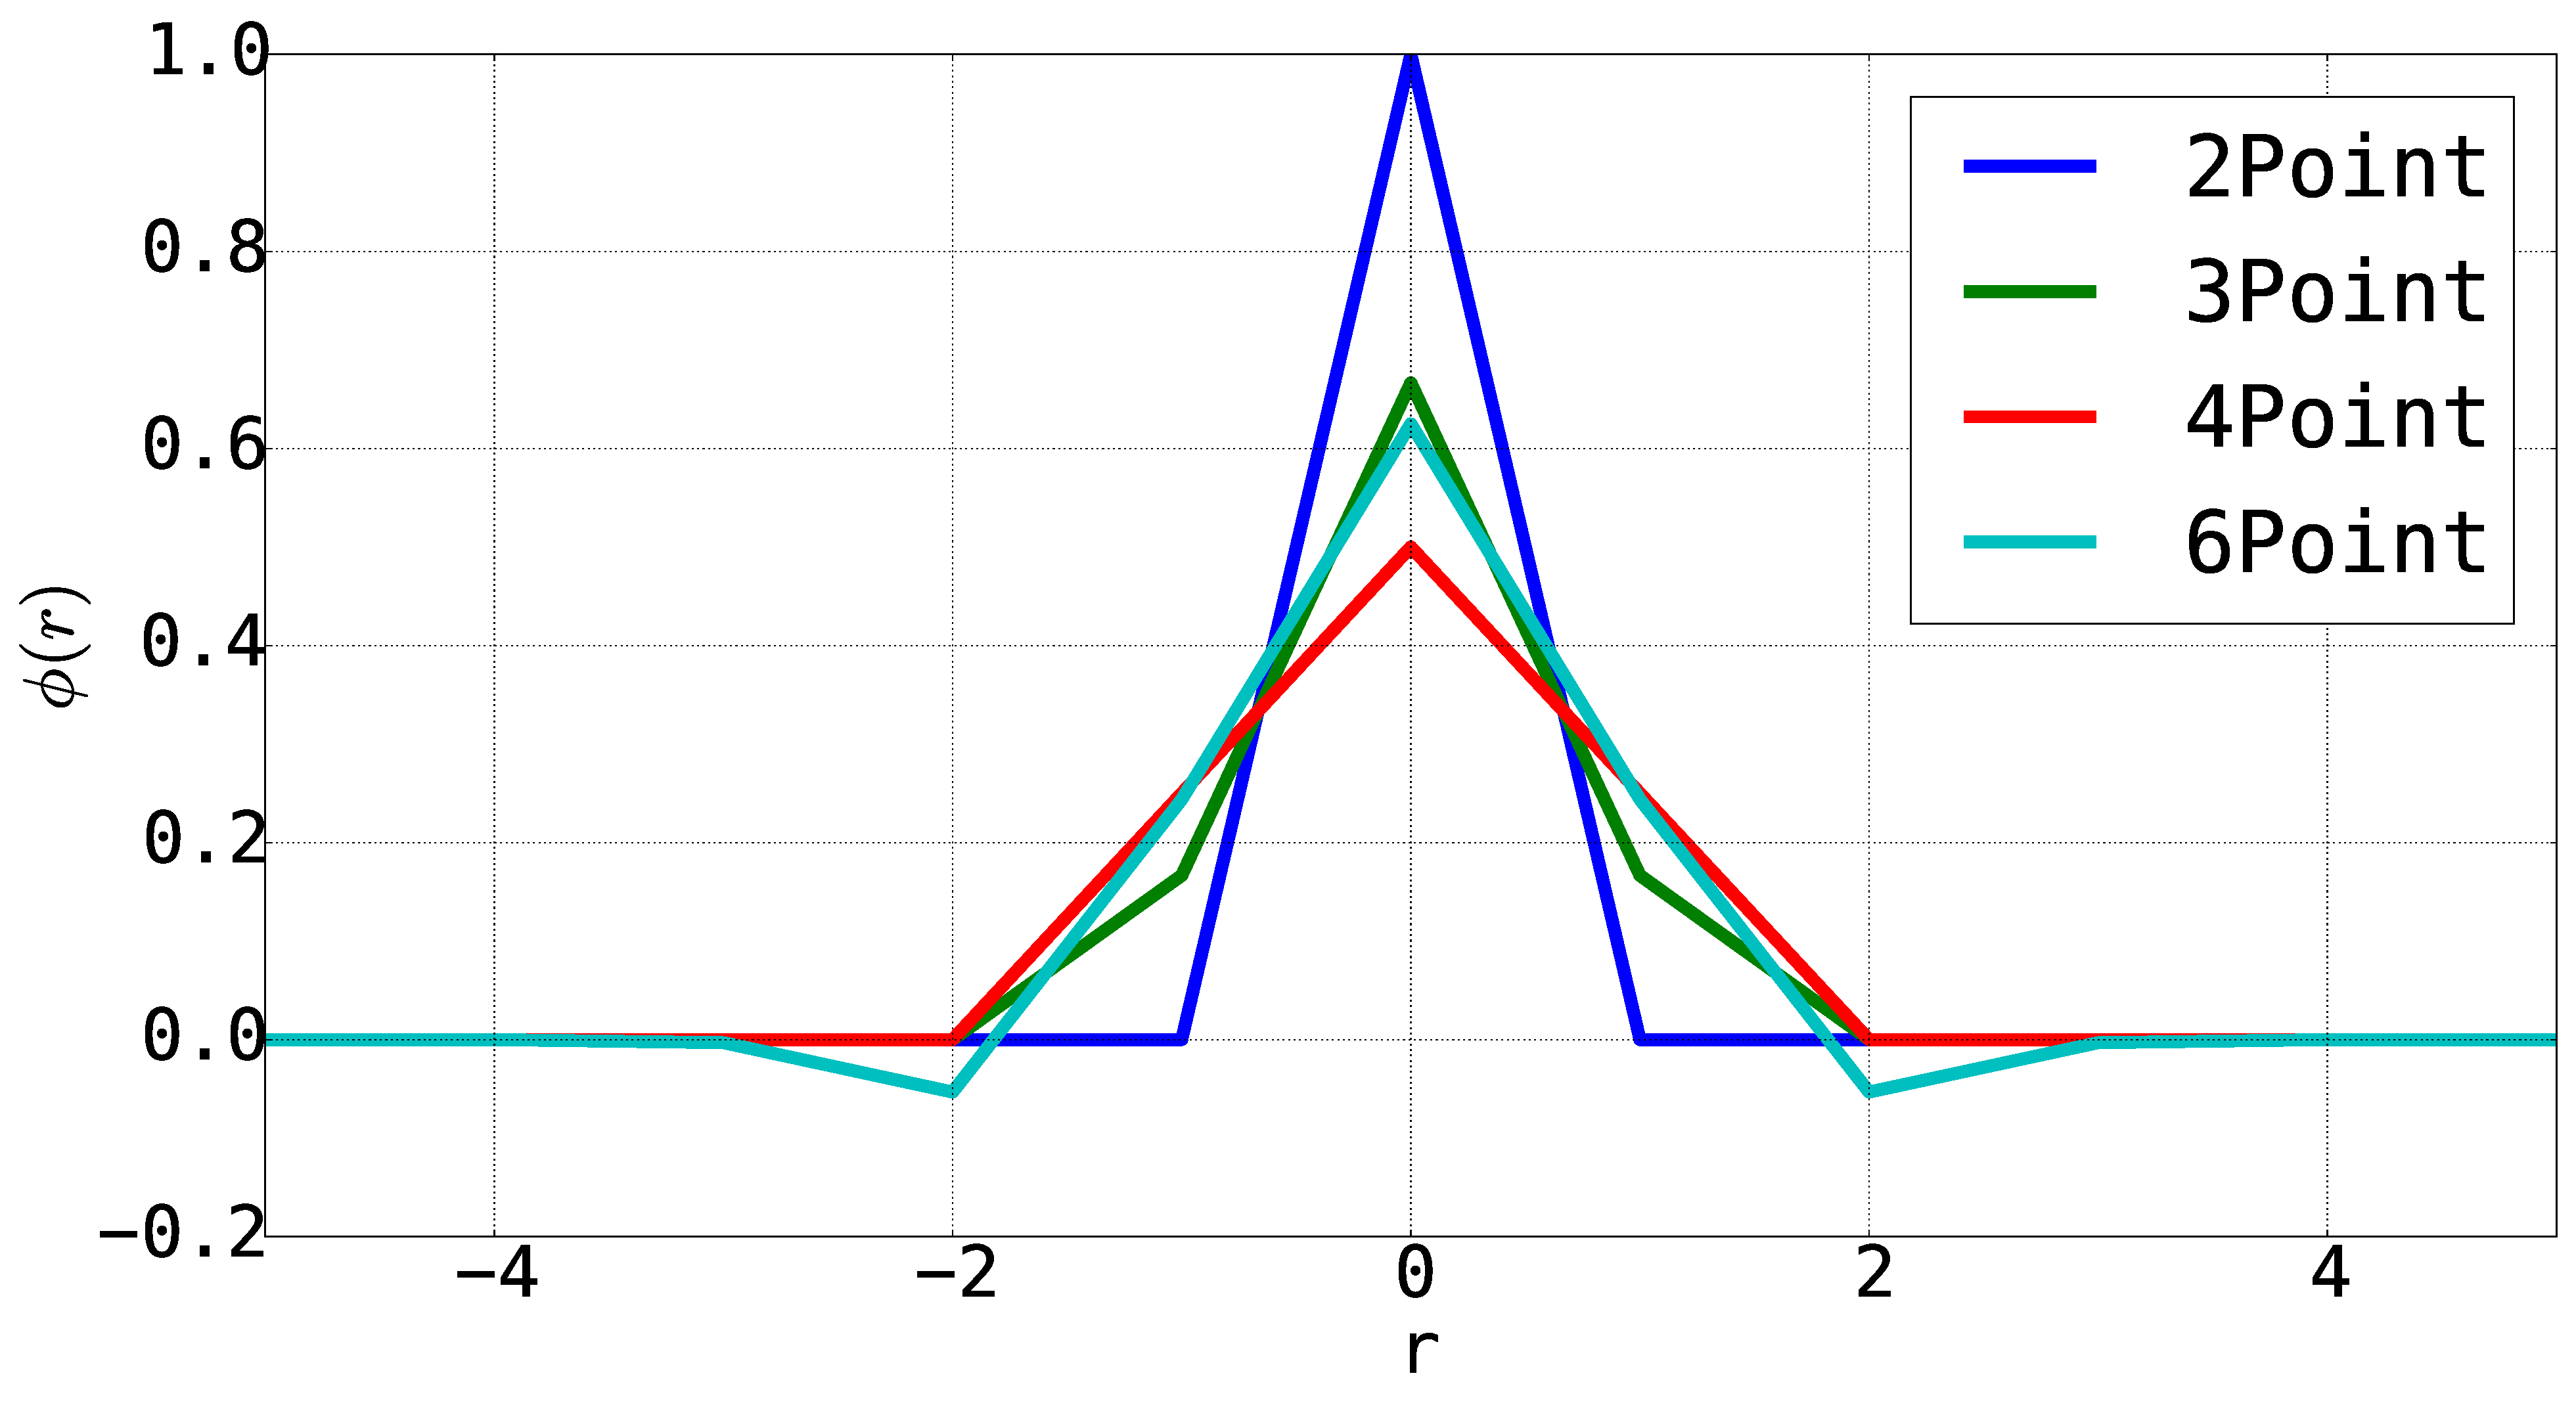
\includegraphics[width=14.cm]{Chapter_3/figure/phi_function.eps}
	\caption{Comparison between different formulations for $\phi$}
\end{figure}

Now we can write the mapping from the Eulerian nodes of the fluid solver to Lagrangian nodes as shown in Equation \eqref{eq:C3_lagrange2euler}.

\begin{equation}\label{eq:C3_lagrange2euler}
	u(X_k) = \int_\Omega u(x) \delta(x - X_k) dx
\end{equation}

where $\Omega$ is the computational domain, $u(x)$ is the velocity at the Eulerian nodes, $x$ is the coordinate of the Eulerian nodes, $u(X_k)$ is the velocity at the desired Lagrangian node, and $X_k$ is the coordinate of the Lagrangian node. Most of the continuum forcing approaches are the same upto this point. They diverge depending of the way they calculate the forcing terms.

% -.-.-.-.-.-.-.-.-.-.-.-.-.-.-.-.-.-.-.-.-.-.-.-.-.-.-.-.-.-.-.-.-.-Classical IB method
\subsection{Classical IB method}
In the classical IB method, the forces at the immersed boundaries are calculate using appropriate constitutive laws, i.e. Hooks law. This can be expressed as follows.

\begin{equation}
	f(X_k) = \mathcal{M}(X_k)
\end{equation}

where $\mathcal{M}$ is an operator which describes the properties of the boundaries. This force is calculated at the Lagrangian points and need to be transferred back to the Eulerian nodes. This is done using the same delta functions used previously to map the Eulerian results to Lagrangian. This method is well suited for a case of elastic bodies but will break for the cases of rigid boundaries or when the rigidity of boundaries are much more than the fluid. The origin of this problem is due to the high cycle oscillations that occur near the boundaries.

This approach is applied to the demonstration problem defined in Section \ref{sec:C3_benchmark_case}. We modelled the location of the fixed boundary using the classical IB method and verified the results using analytical formulas for this problem. The forcing function is added to the right-hand-side of the governing equation as follows

\begin{equation}
	\frac{\partial u}{\partial t} = \frac{\partial^2 u}{\partial y^2} - f(t)
\end{equation}

where $f(t)$ is the forcing function using to model the boundary. This equation is discretized using the Cranck-Nicholson method as follows

\begin{equation}\label{eq:C3_discretizedEquationPeskinIB}
	u^{n+1} = u^{n} + \frac{\Delta t}{2} \left( \frac{\partial^2 u^{n+1}}{\partial x^2} + 
	                                            \frac{\partial^2 u^n}{\partial x^2}\right) - \Delta t f^n 
\end{equation}

The steps to solve this equation and model the stationary wall using the IB method are as follows

\begin{enumerate}
	\item Define the initial condition as $u^0$ and set $f^0$ equal to zero.
	\item Calculate the velocity at the next time step, $u^1$, using Equation \eqref{eq:C3_discretizedEquationPeskinIB}
	\item Based on the new velocity at $t=1$ calculate the velocity at the location where the stationary wall is supposed to be, $X$, using $\delta$ function ($U$).
	\item Calculate the distance that this node will move in the current time step: $X^{n+1} = X^n + U \Delta t$
	\item Based on the new location of the node, calculate the forces as: $F = K \left( X^{n+1} - X^0 \right)$, where $X^0$ is the desired location of the wall and $K$ is the stiffness of wall. 
	\item Map the force at the Lagrangian location $X$ to its neighbouring Eulerian points using $\delta$ function.
	\item Reiterate until the convergence is satisfied.
\end{enumerate}

For the classical IB method, we investigated the accuracy of the results to the number of nodes, wall velocity, and the stiffness used to model the wall. The immersed boundary simulation is compared with analytical solution of this problem. We chose the normalized root mean square error to compared the analytical and IB results. This is defined as follows.

\begin{equation*}
	NRMSE = \dfrac{\sqrt{\dfrac{\sum_{n=1}{N} \left( \hat{y}_n - y \right)^2}{n}}}{y_{max} - y_{min}}
\end{equation*}

where $\hat{y}_t$ is the predicted value, $y$ is the true value, and $n$ is the number data points. Normalizing by $y_{max} - y_{min}$ enables us to compare models with different scales. This is especially useful when compared the results for different wall velocities.

For the first investigation, we selected the wall stiffness as $10^2$ and its location is selected as $x_{wall} = 0.51885$. We chose this location so that it does not coincide with the location of computational nodes. The time step is chosen as $10^{-5}$ and the wall velocity is fixed at $1 m/s$. For this simulation we used both 2-point and 4-point delta functions to transfer results between Lagrangian and Eulerian nodes. The computation domain is discretized using $11$, $41$, $81$, and $161$ nodes. The results of IB method is verified with analytical results.

\begin{figure}[H]
	\centering
	\subfigure[N = 11, 2-point delta function]
	{
	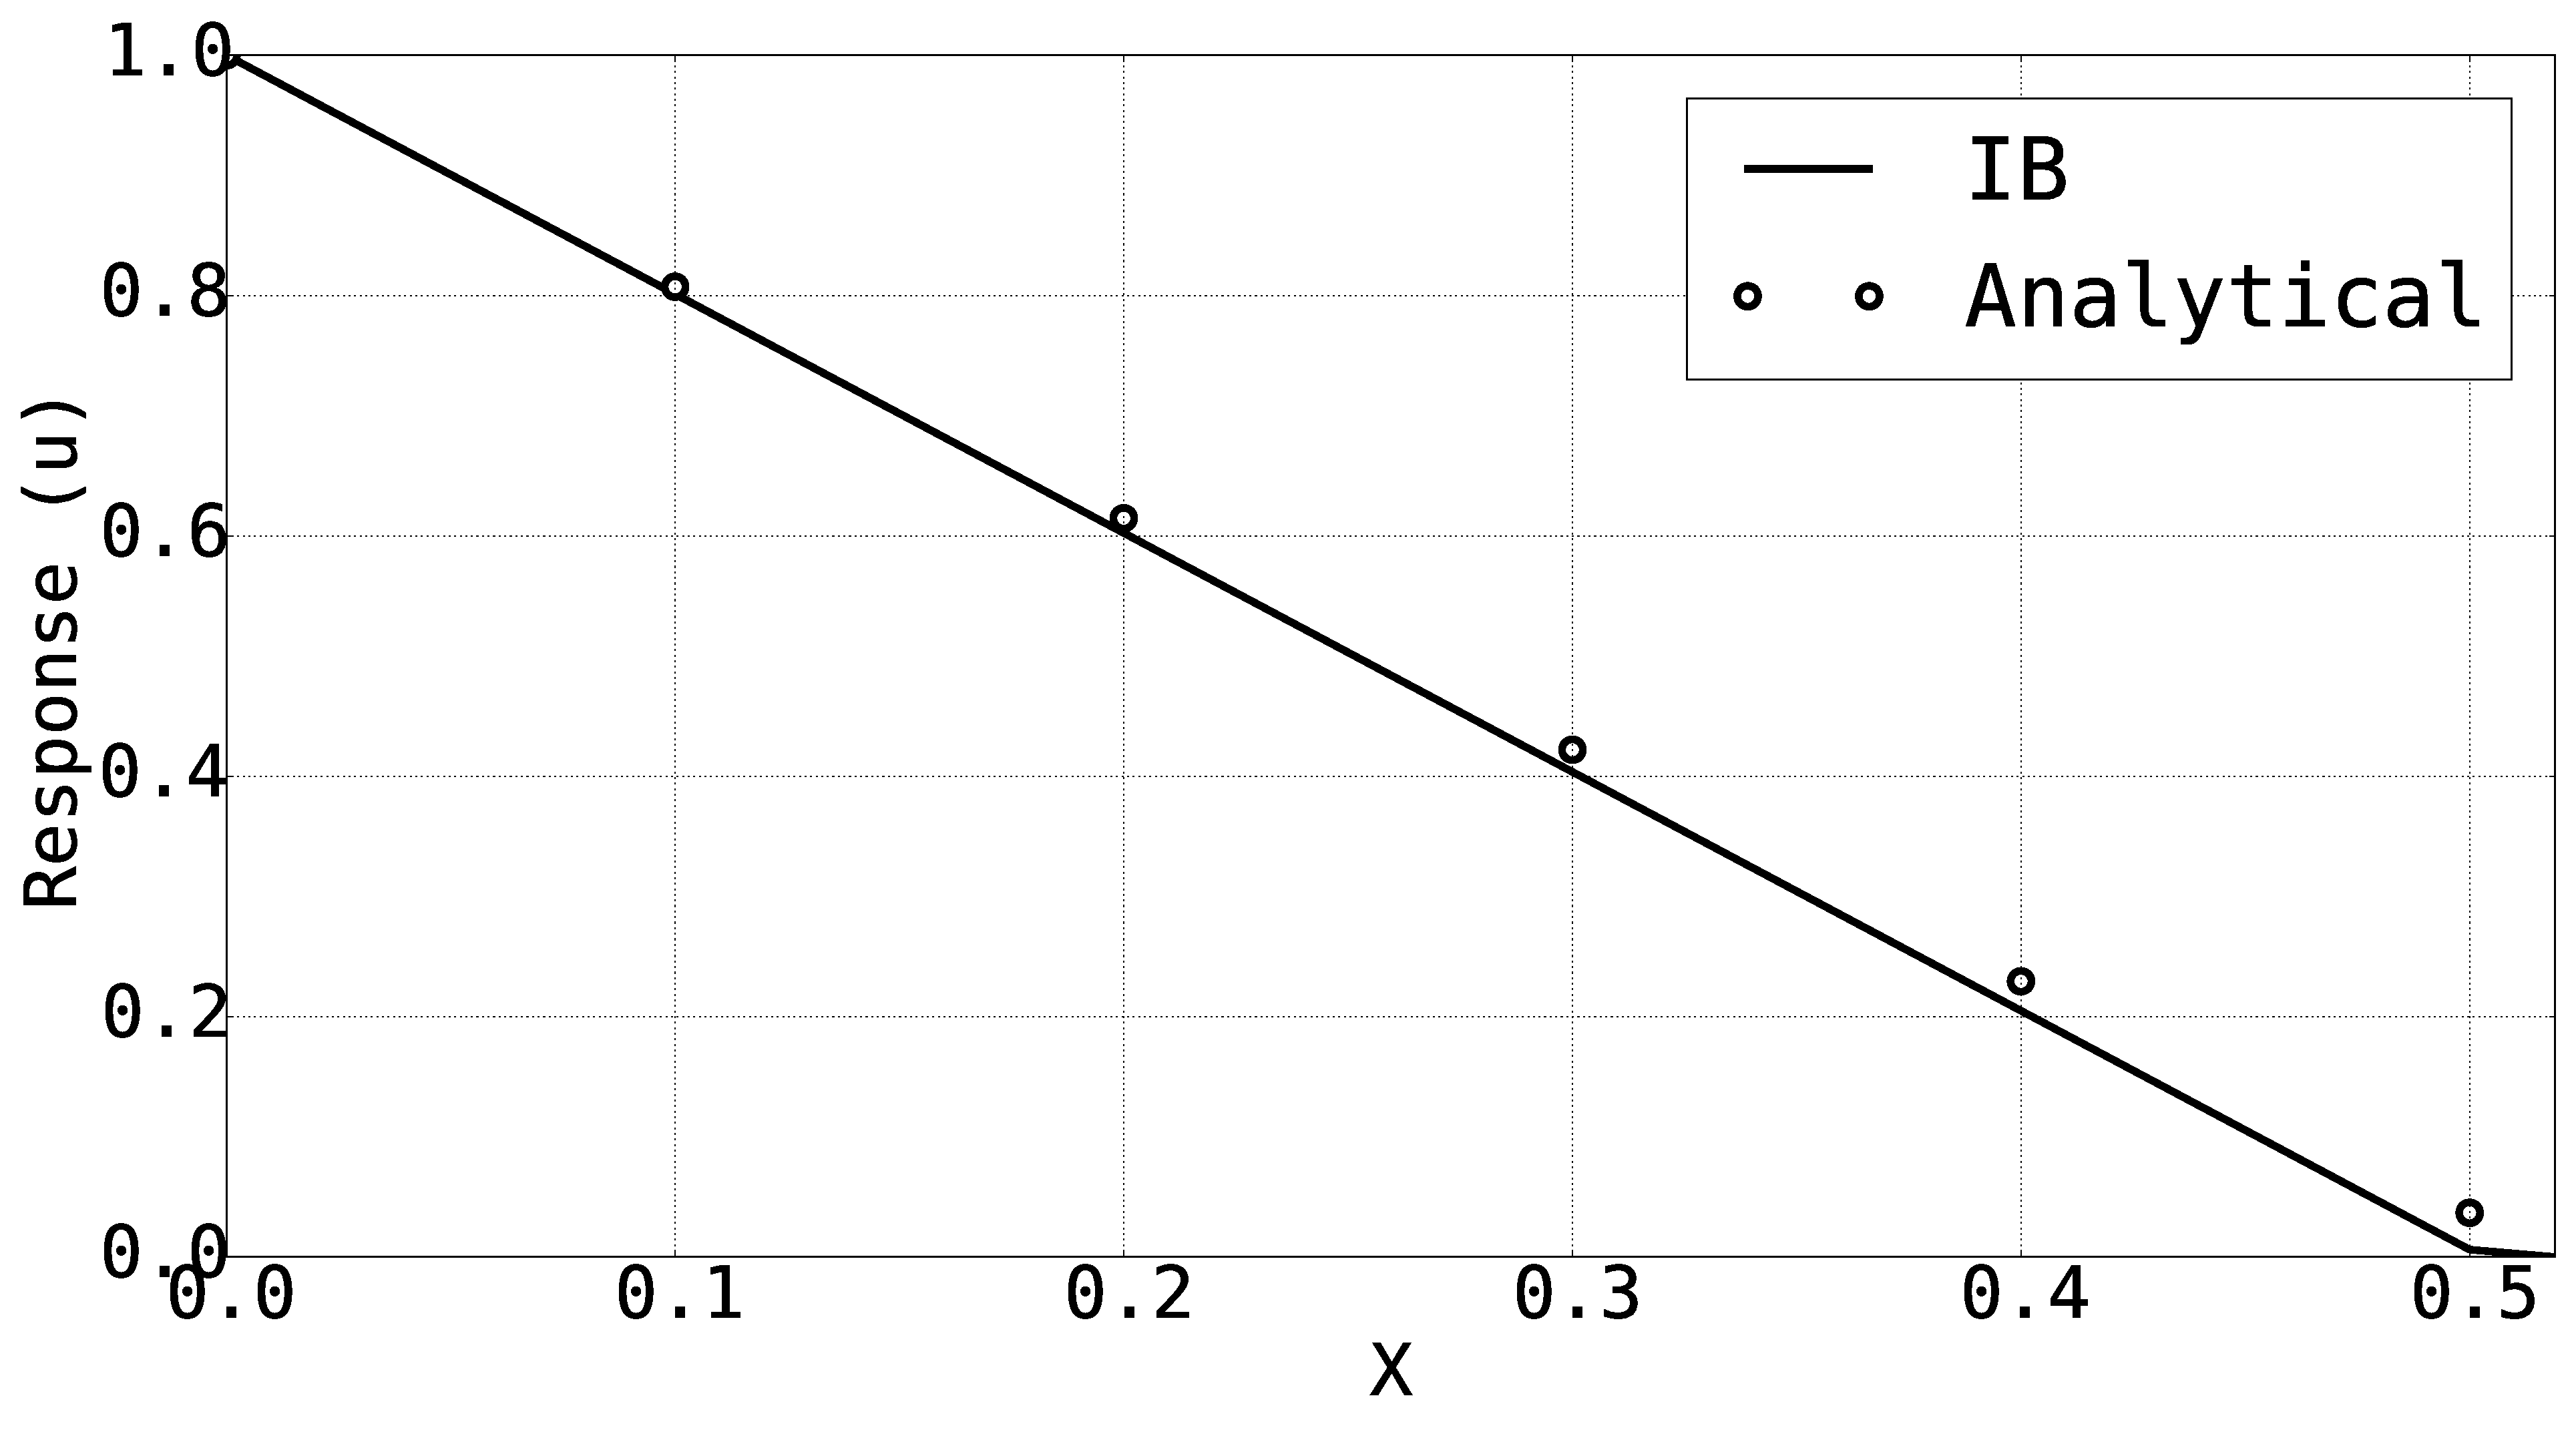
\includegraphics[width=7.0cm]{Chapter_3/figure/classicalIB_nodeNumber_2point_11.eps}
	}
	\quad
	\subfigure[N = 11, 4-point delta function]
	{
	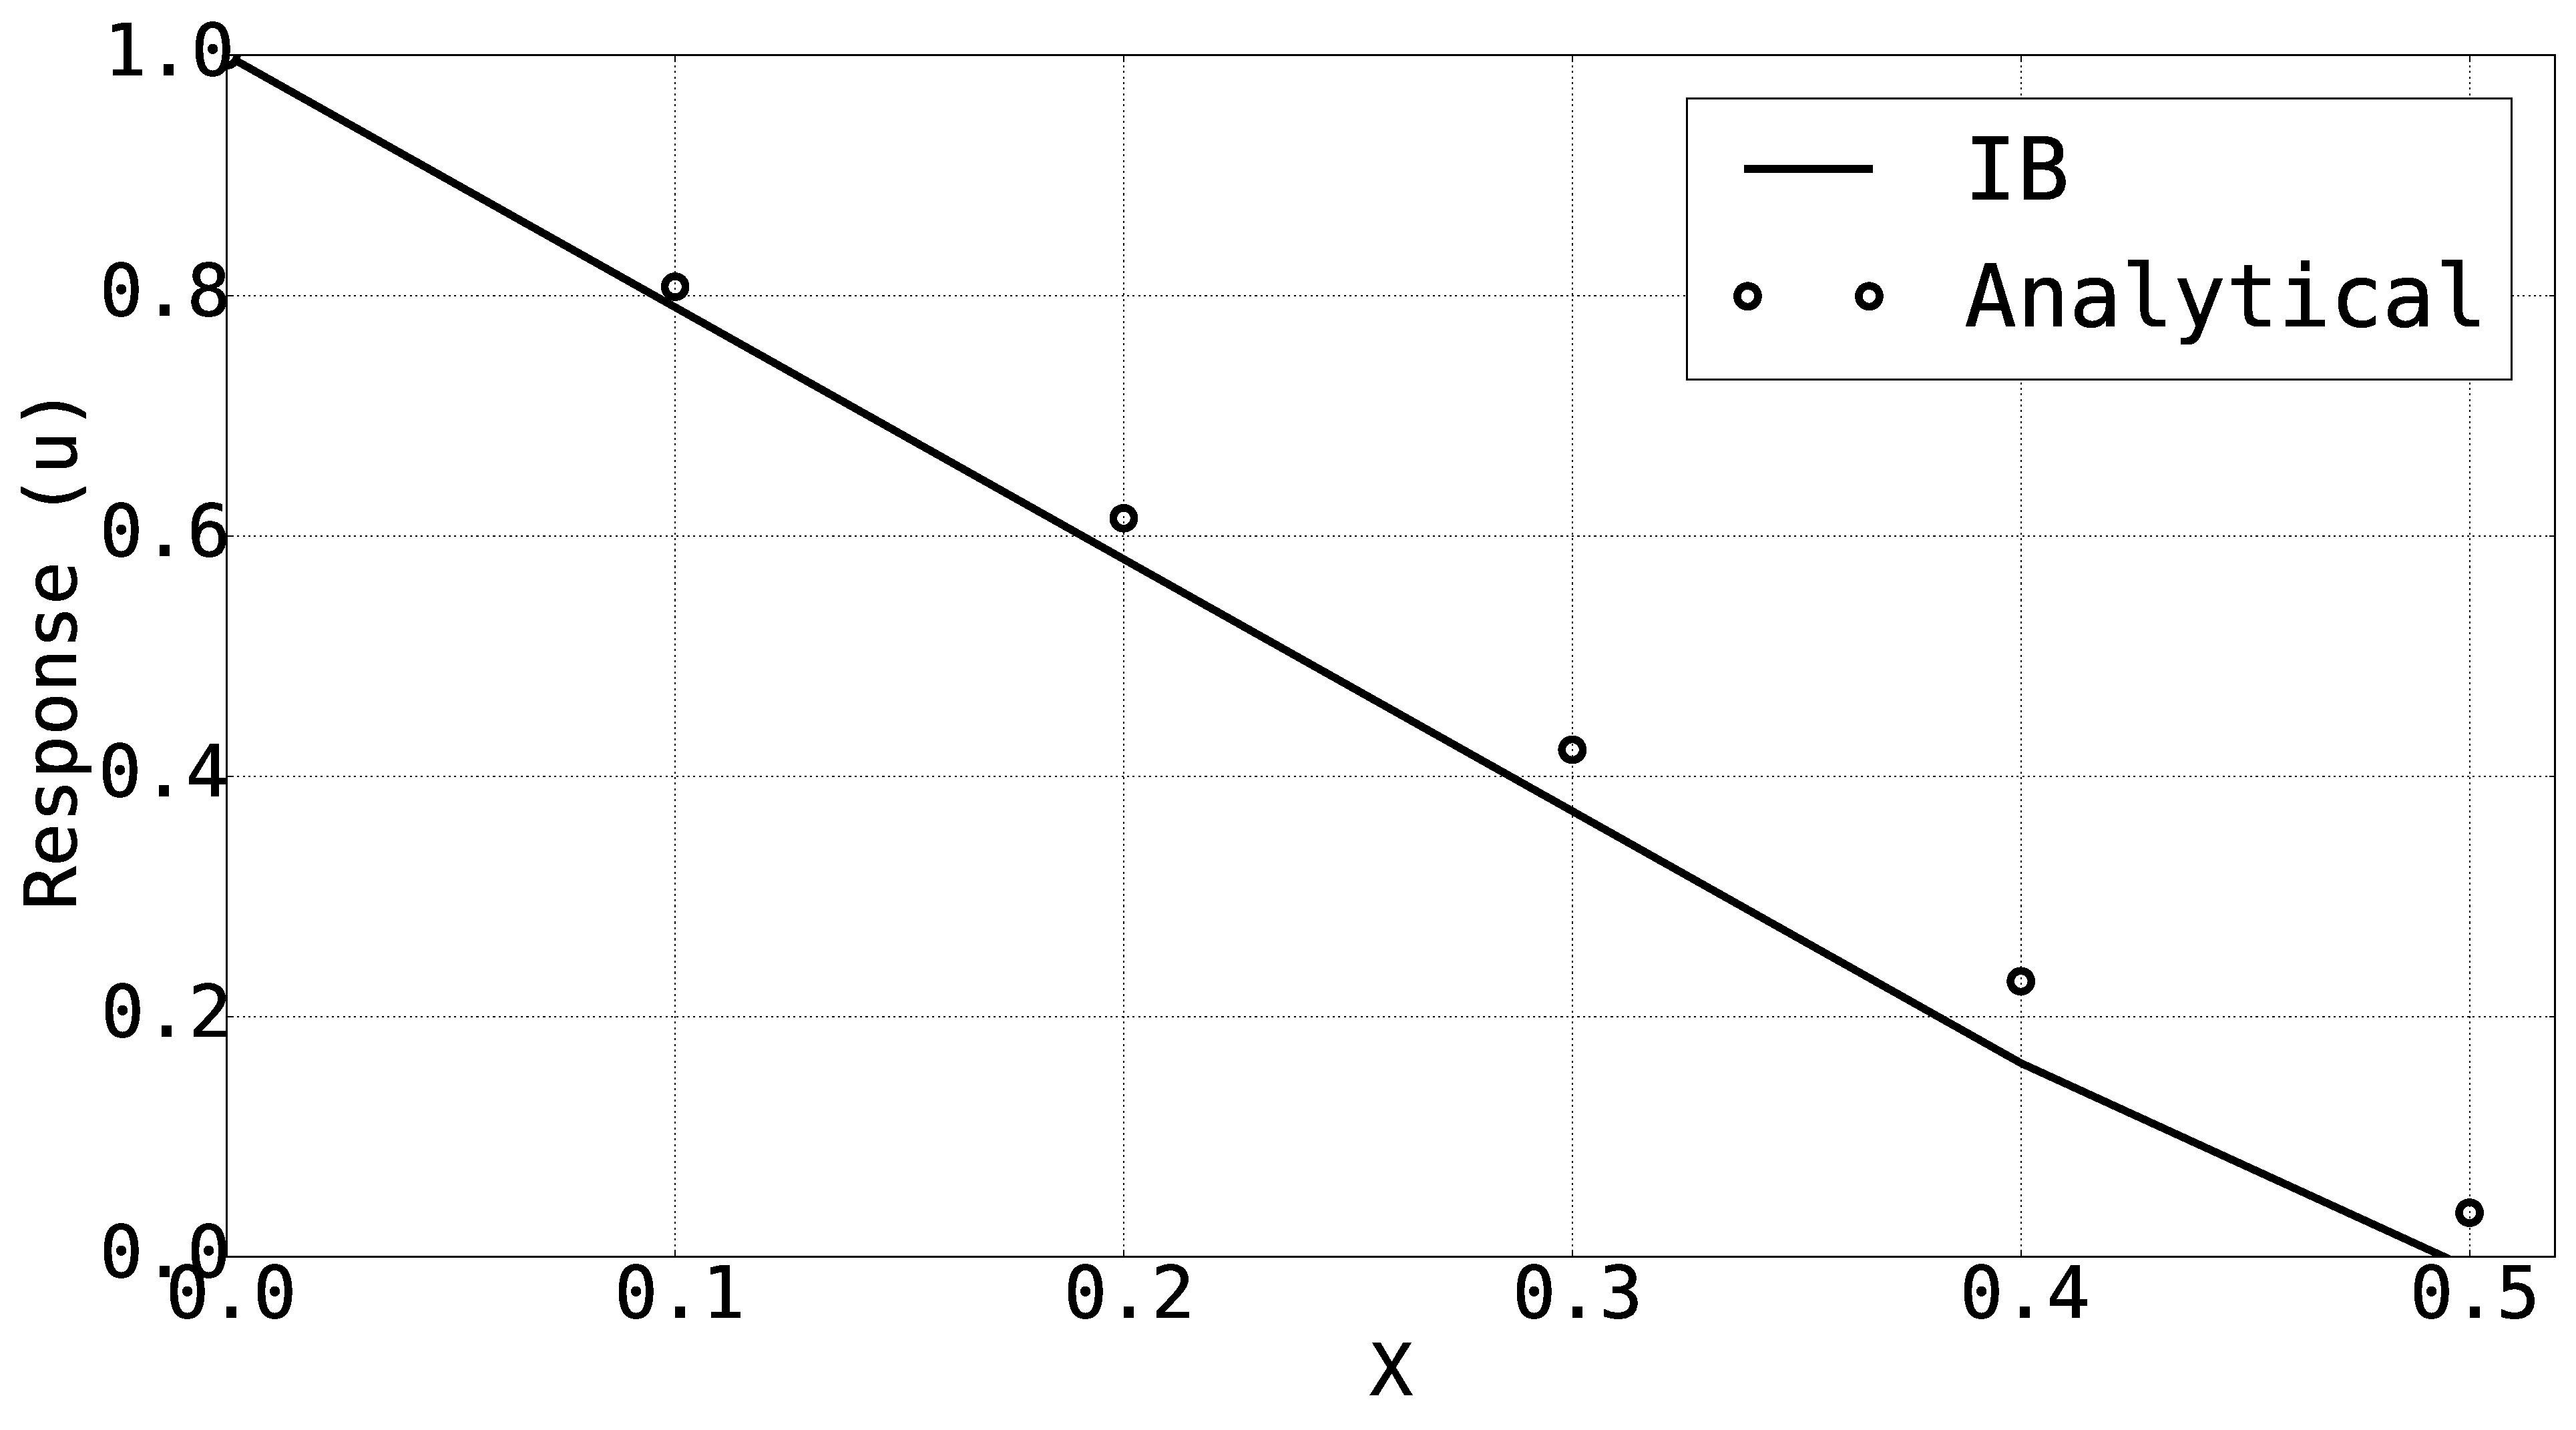
\includegraphics[width=7.0cm]{Chapter_3/figure/classicalIB_nodeNumber_4point_11.eps}
	}
	\\
	\subfigure[N = 41, 2-point delta function]
	{
	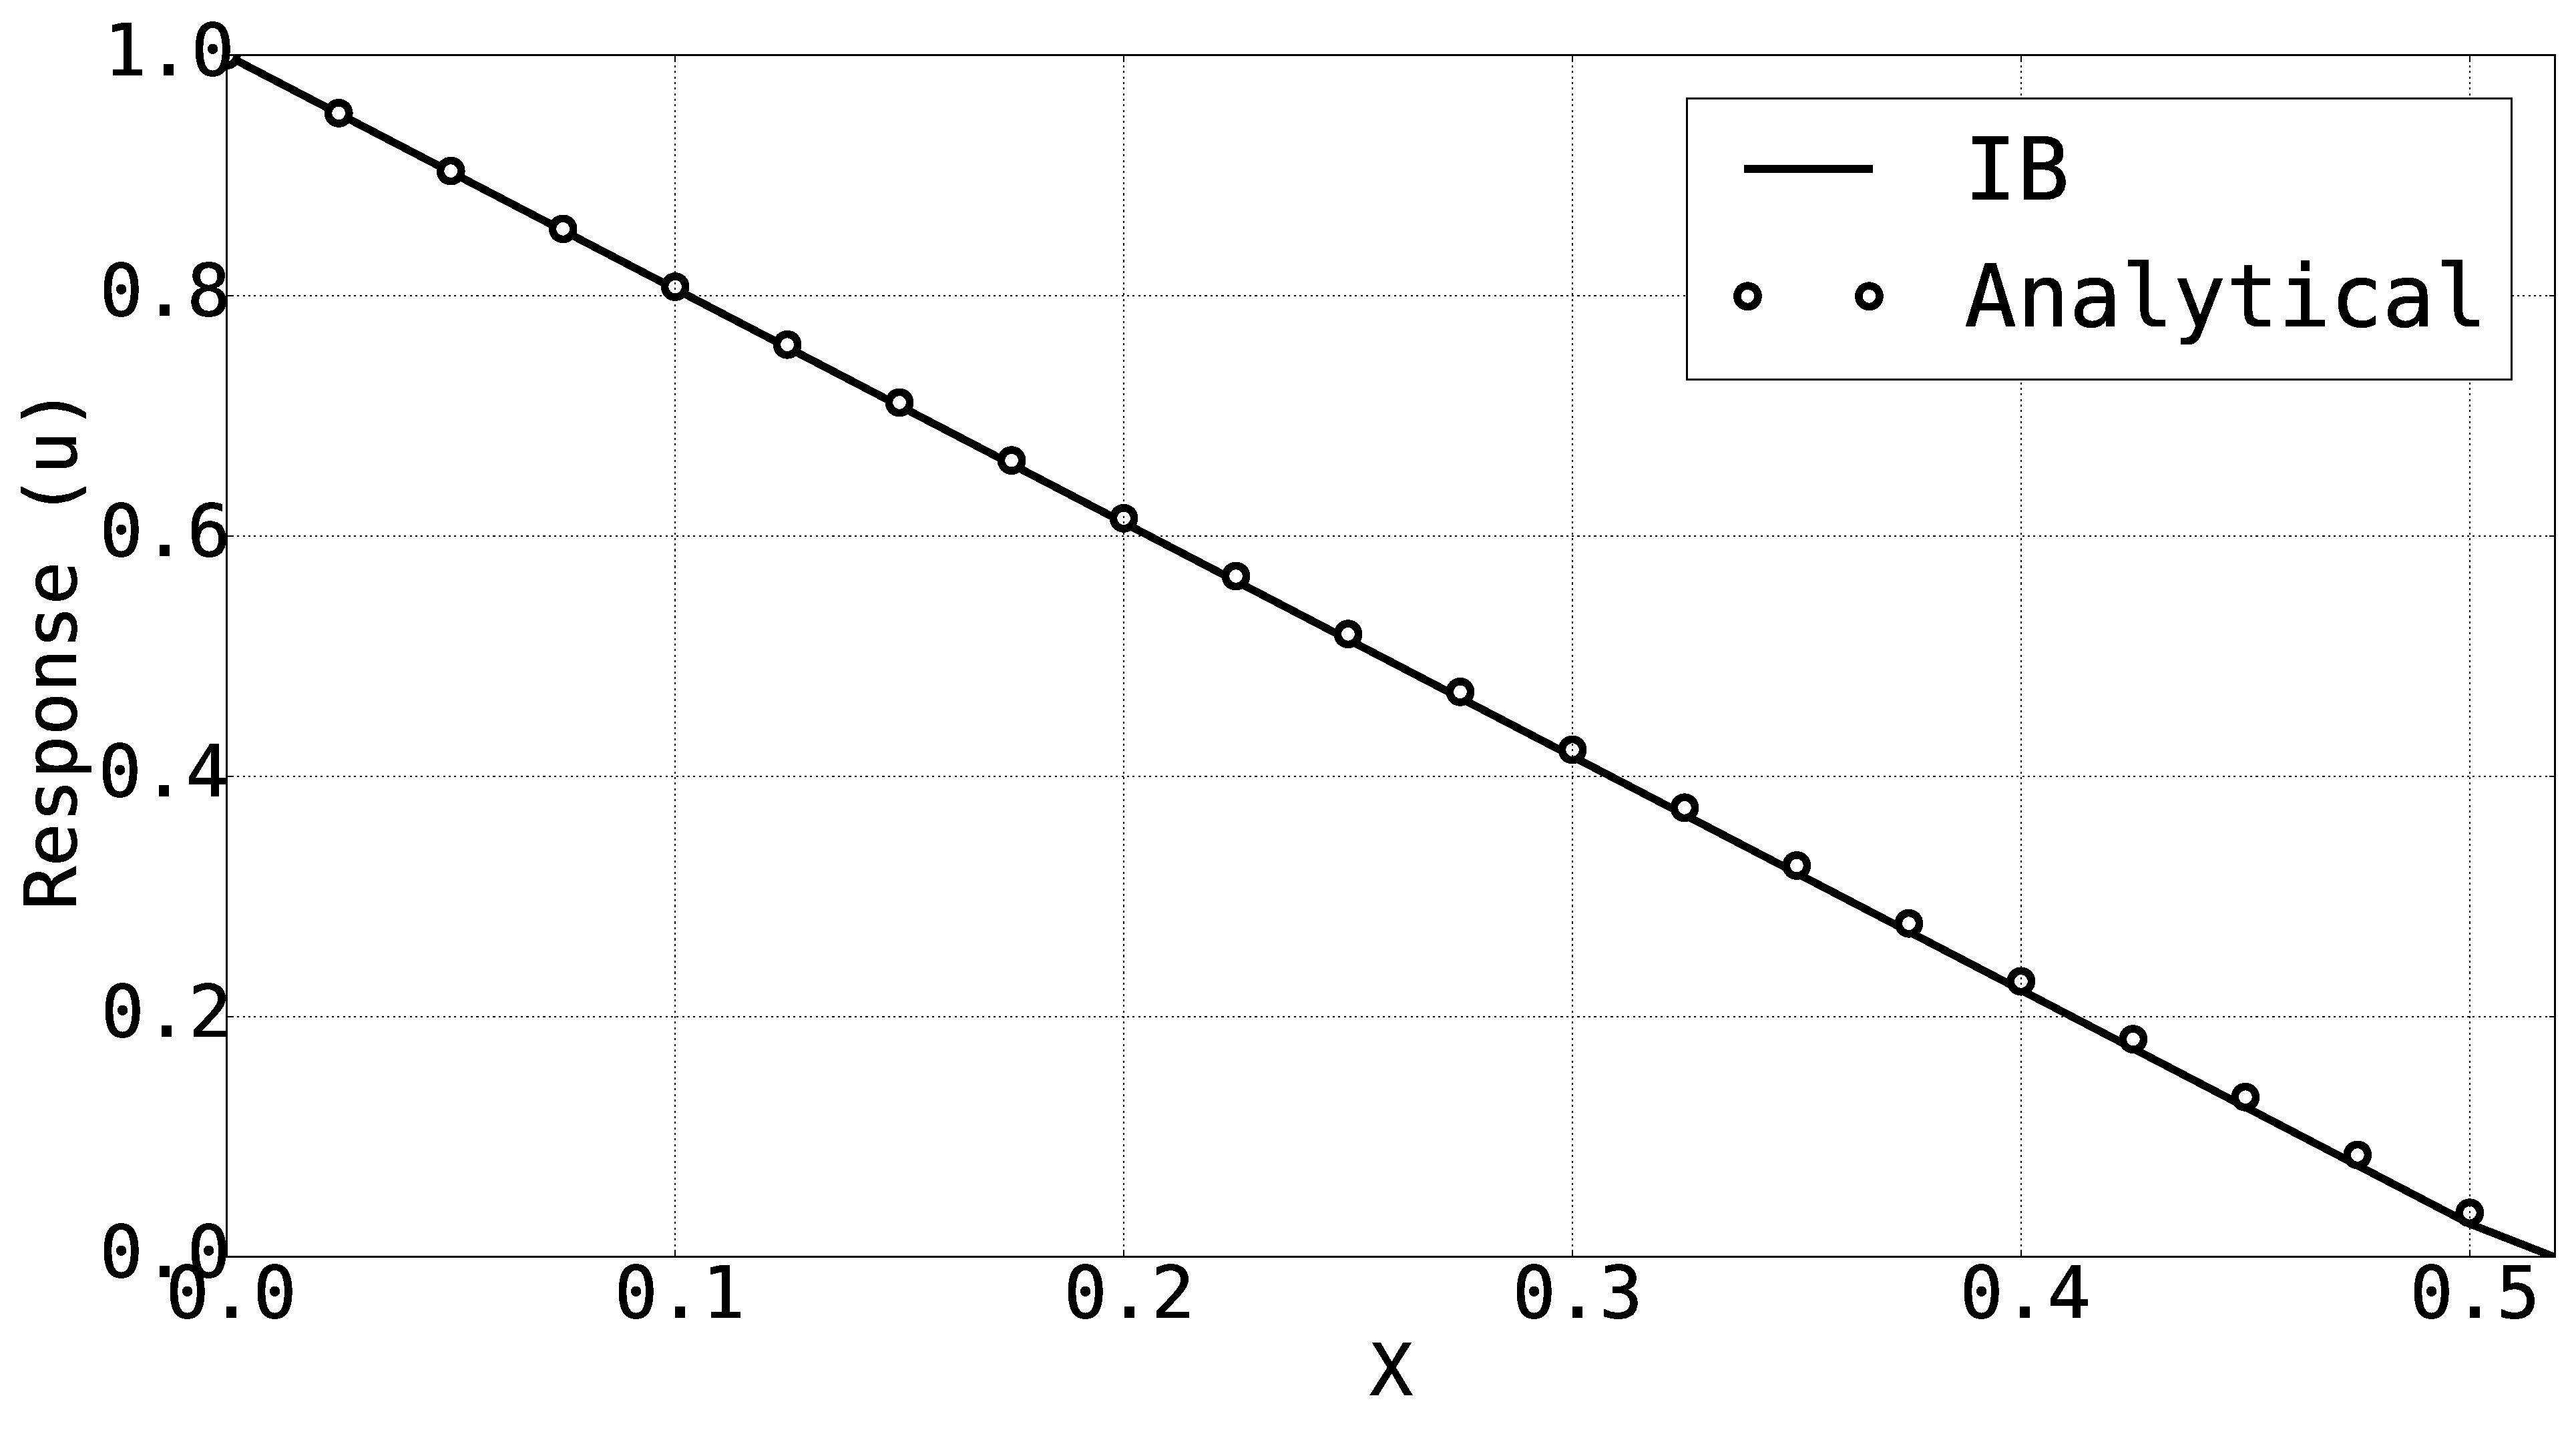
\includegraphics[width=7.0cm]{Chapter_3/figure/classicalIB_nodeNumber_2point_41.eps}
	}
	\quad
	\subfigure[N = 41, 4-point delta function]
	{
	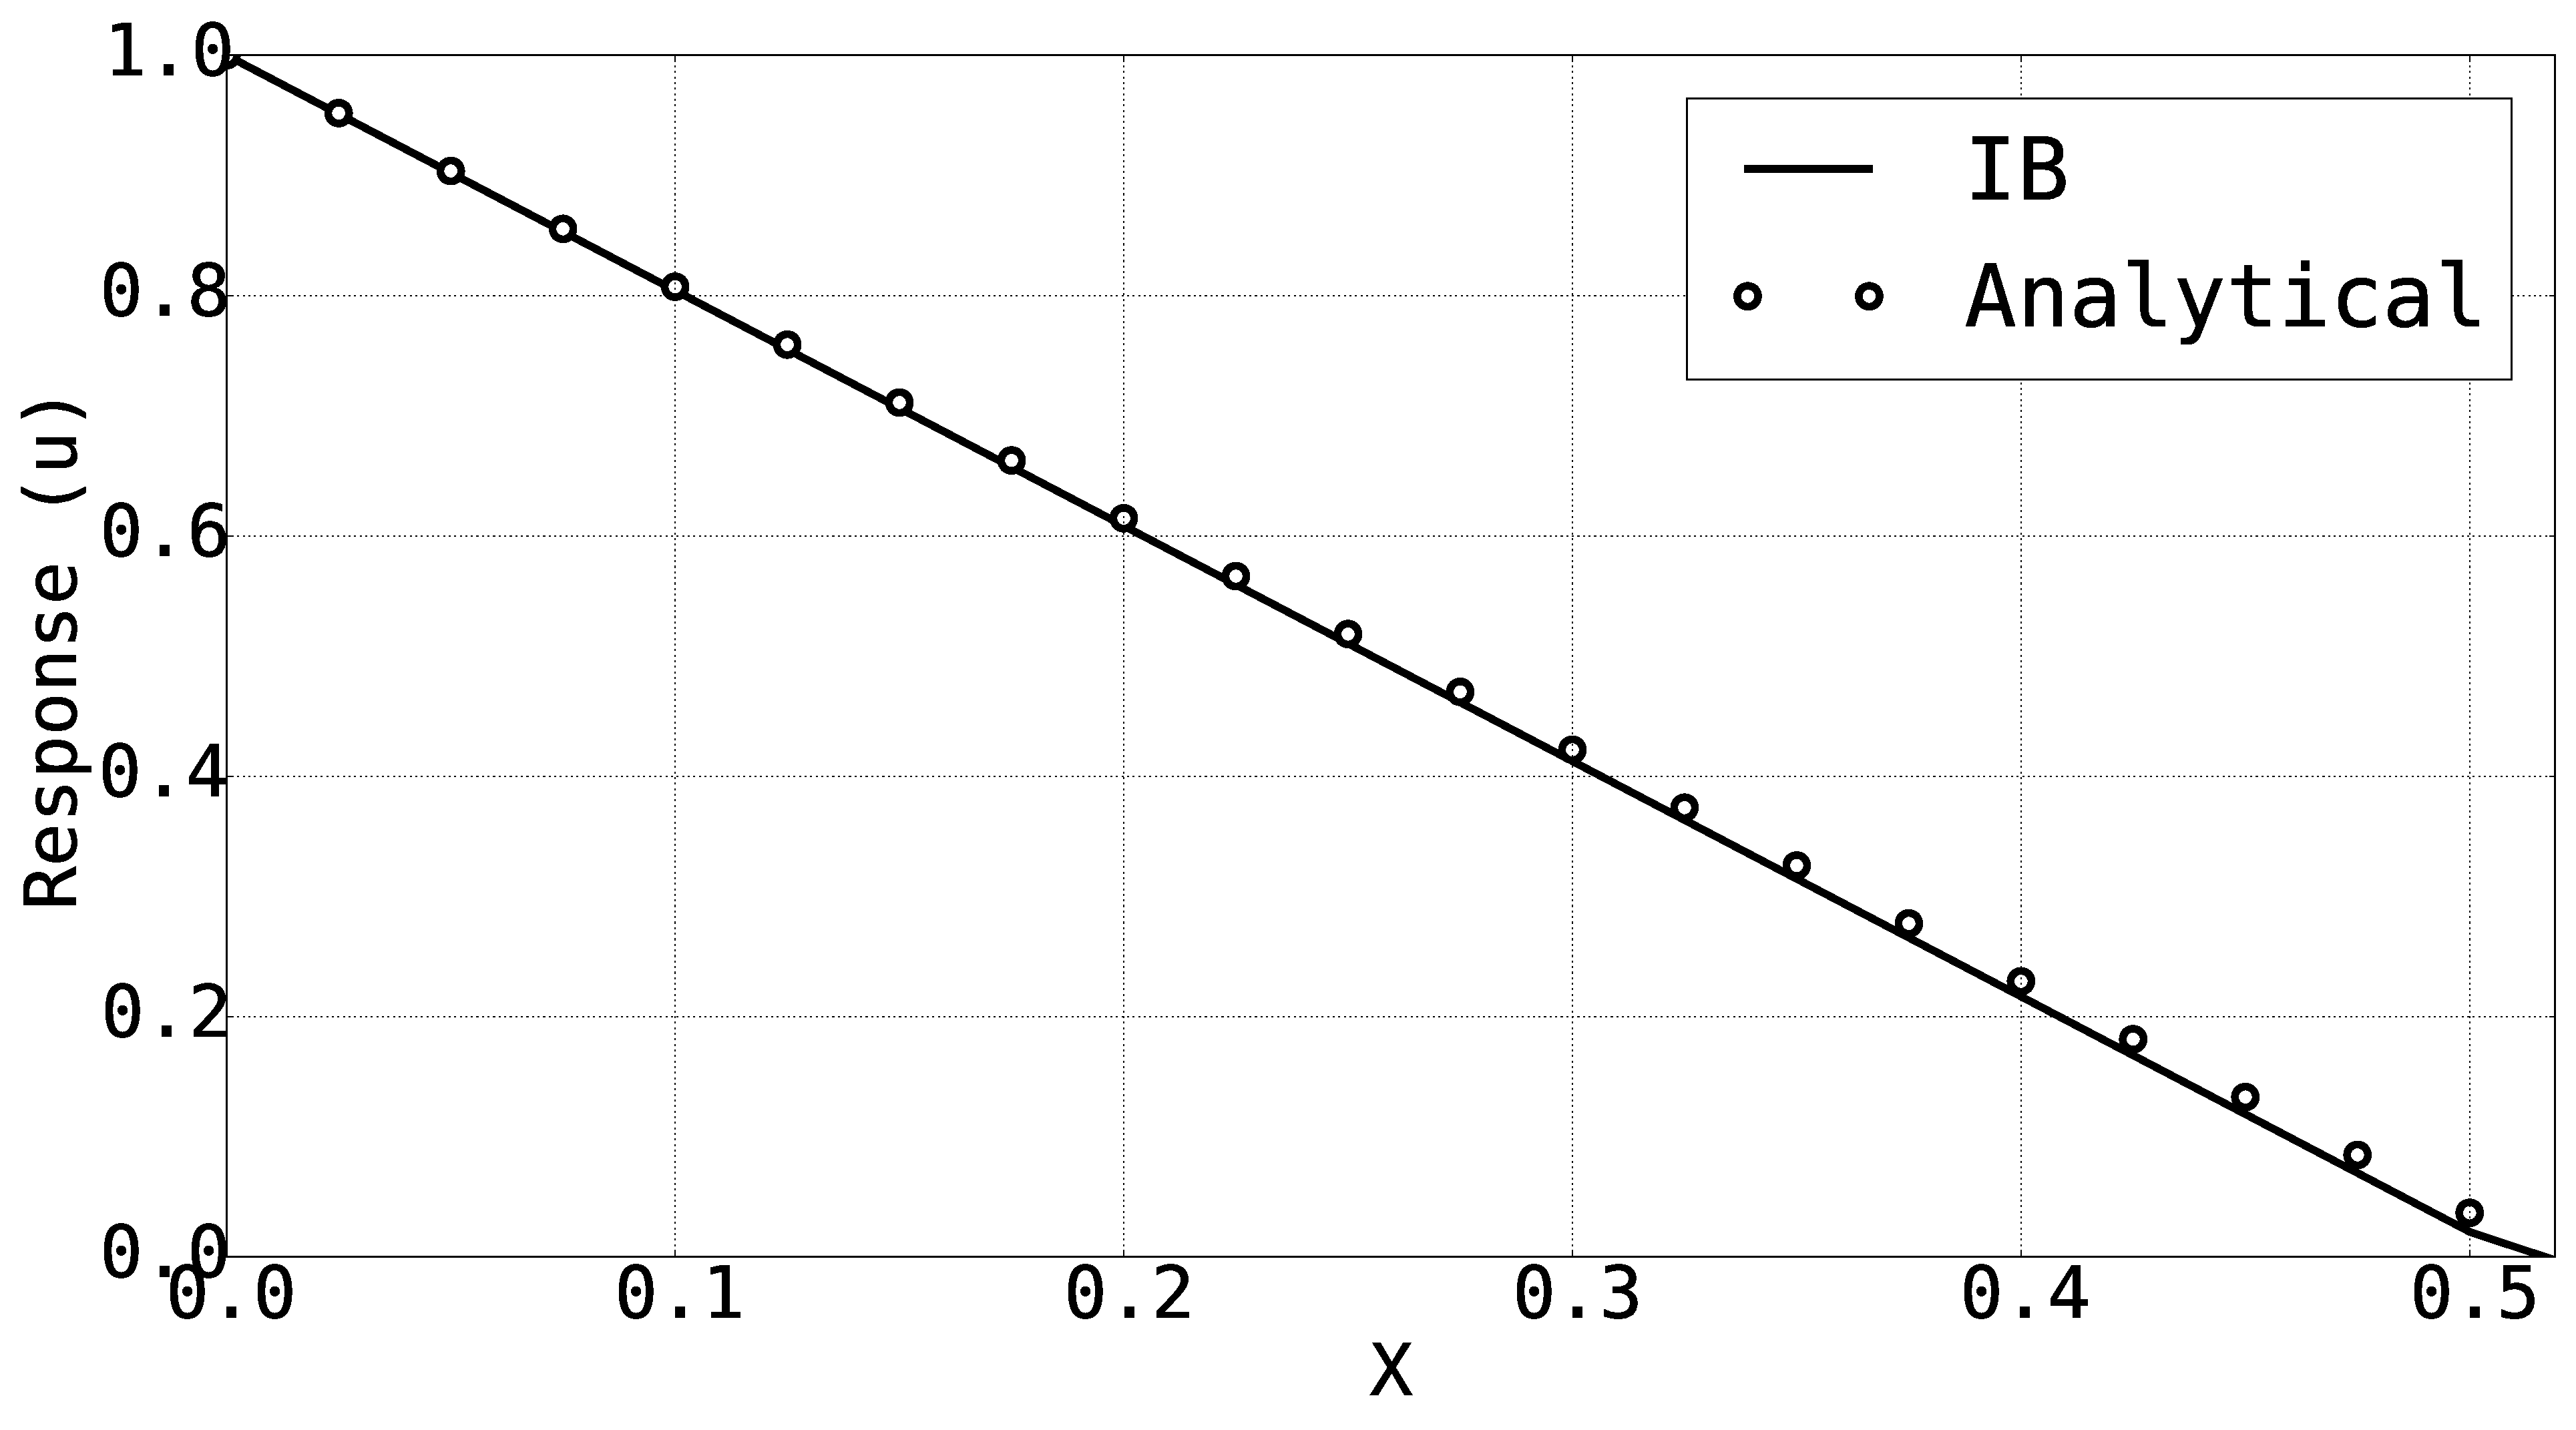
\includegraphics[width=7.0cm]{Chapter_3/figure/classicalIB_nodeNumber_4point_41.eps}
	}
	\\
	\subfigure[N = 81, 2-point delta function]
	{
	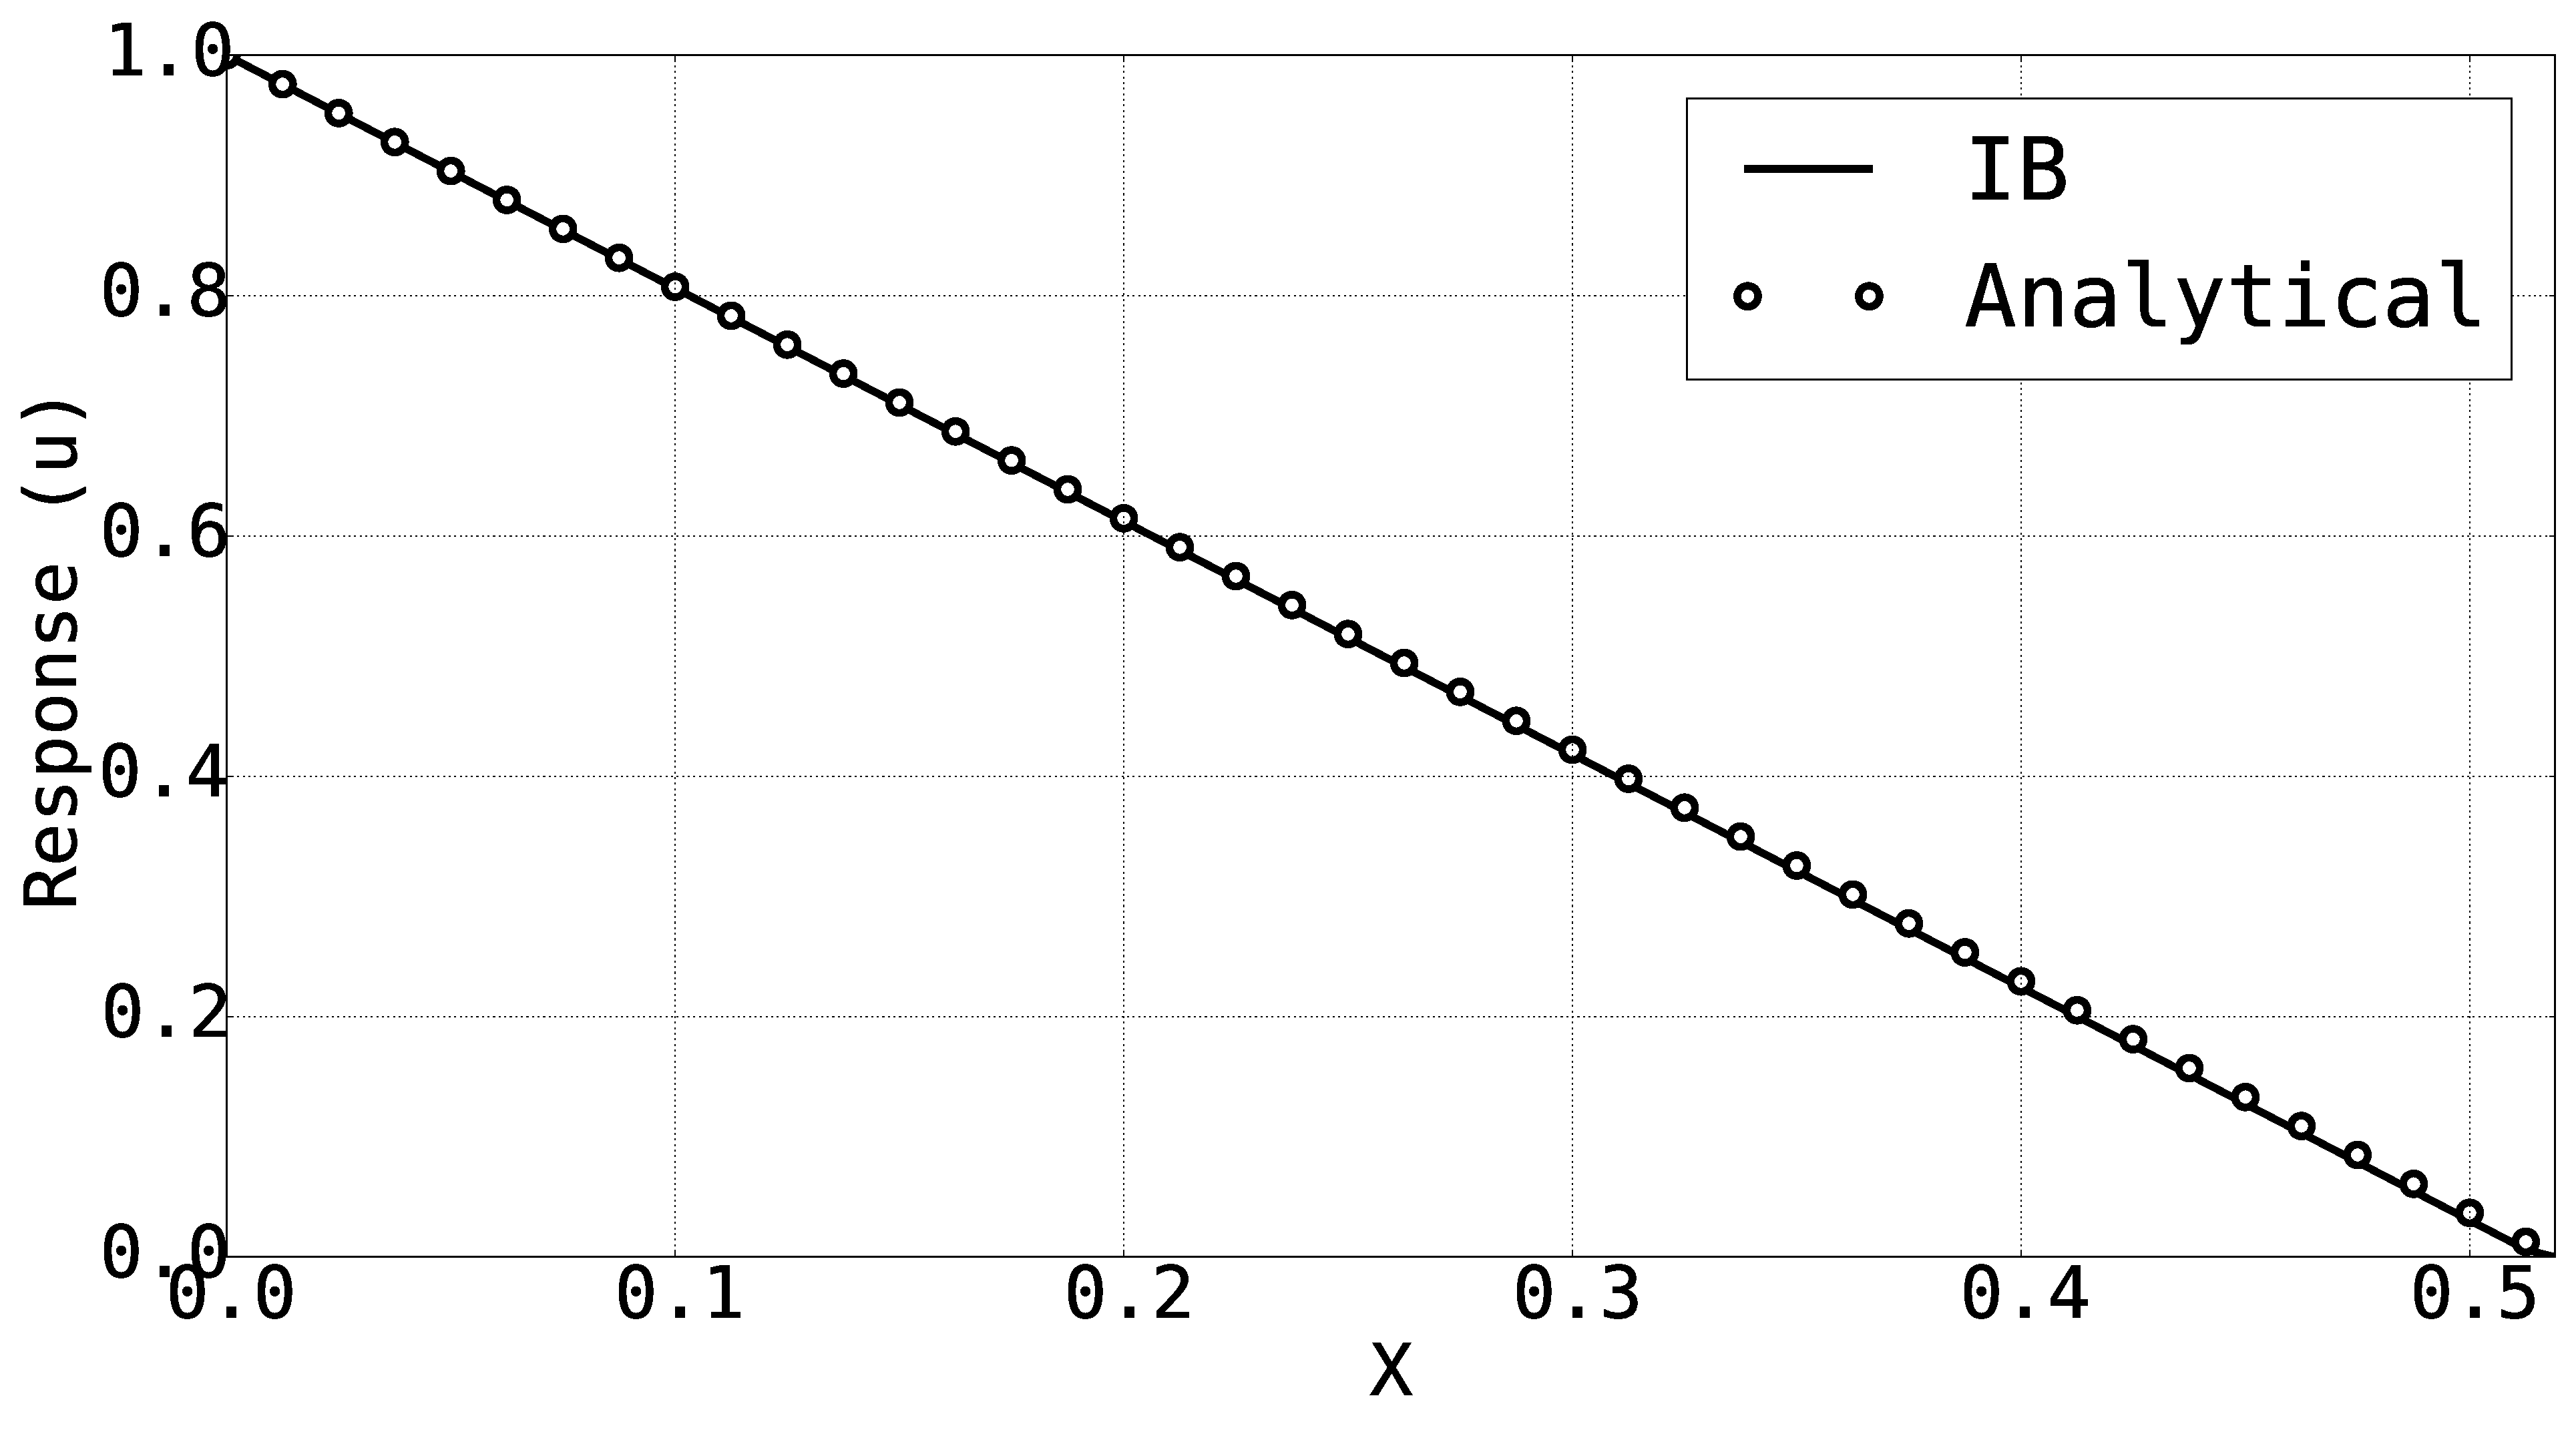
\includegraphics[width=7.0cm]{Chapter_3/figure/classicalIB_nodeNumber_2point_81.eps}
	}
	\quad
	\subfigure[N = 81, 4-point delta function]
	{
	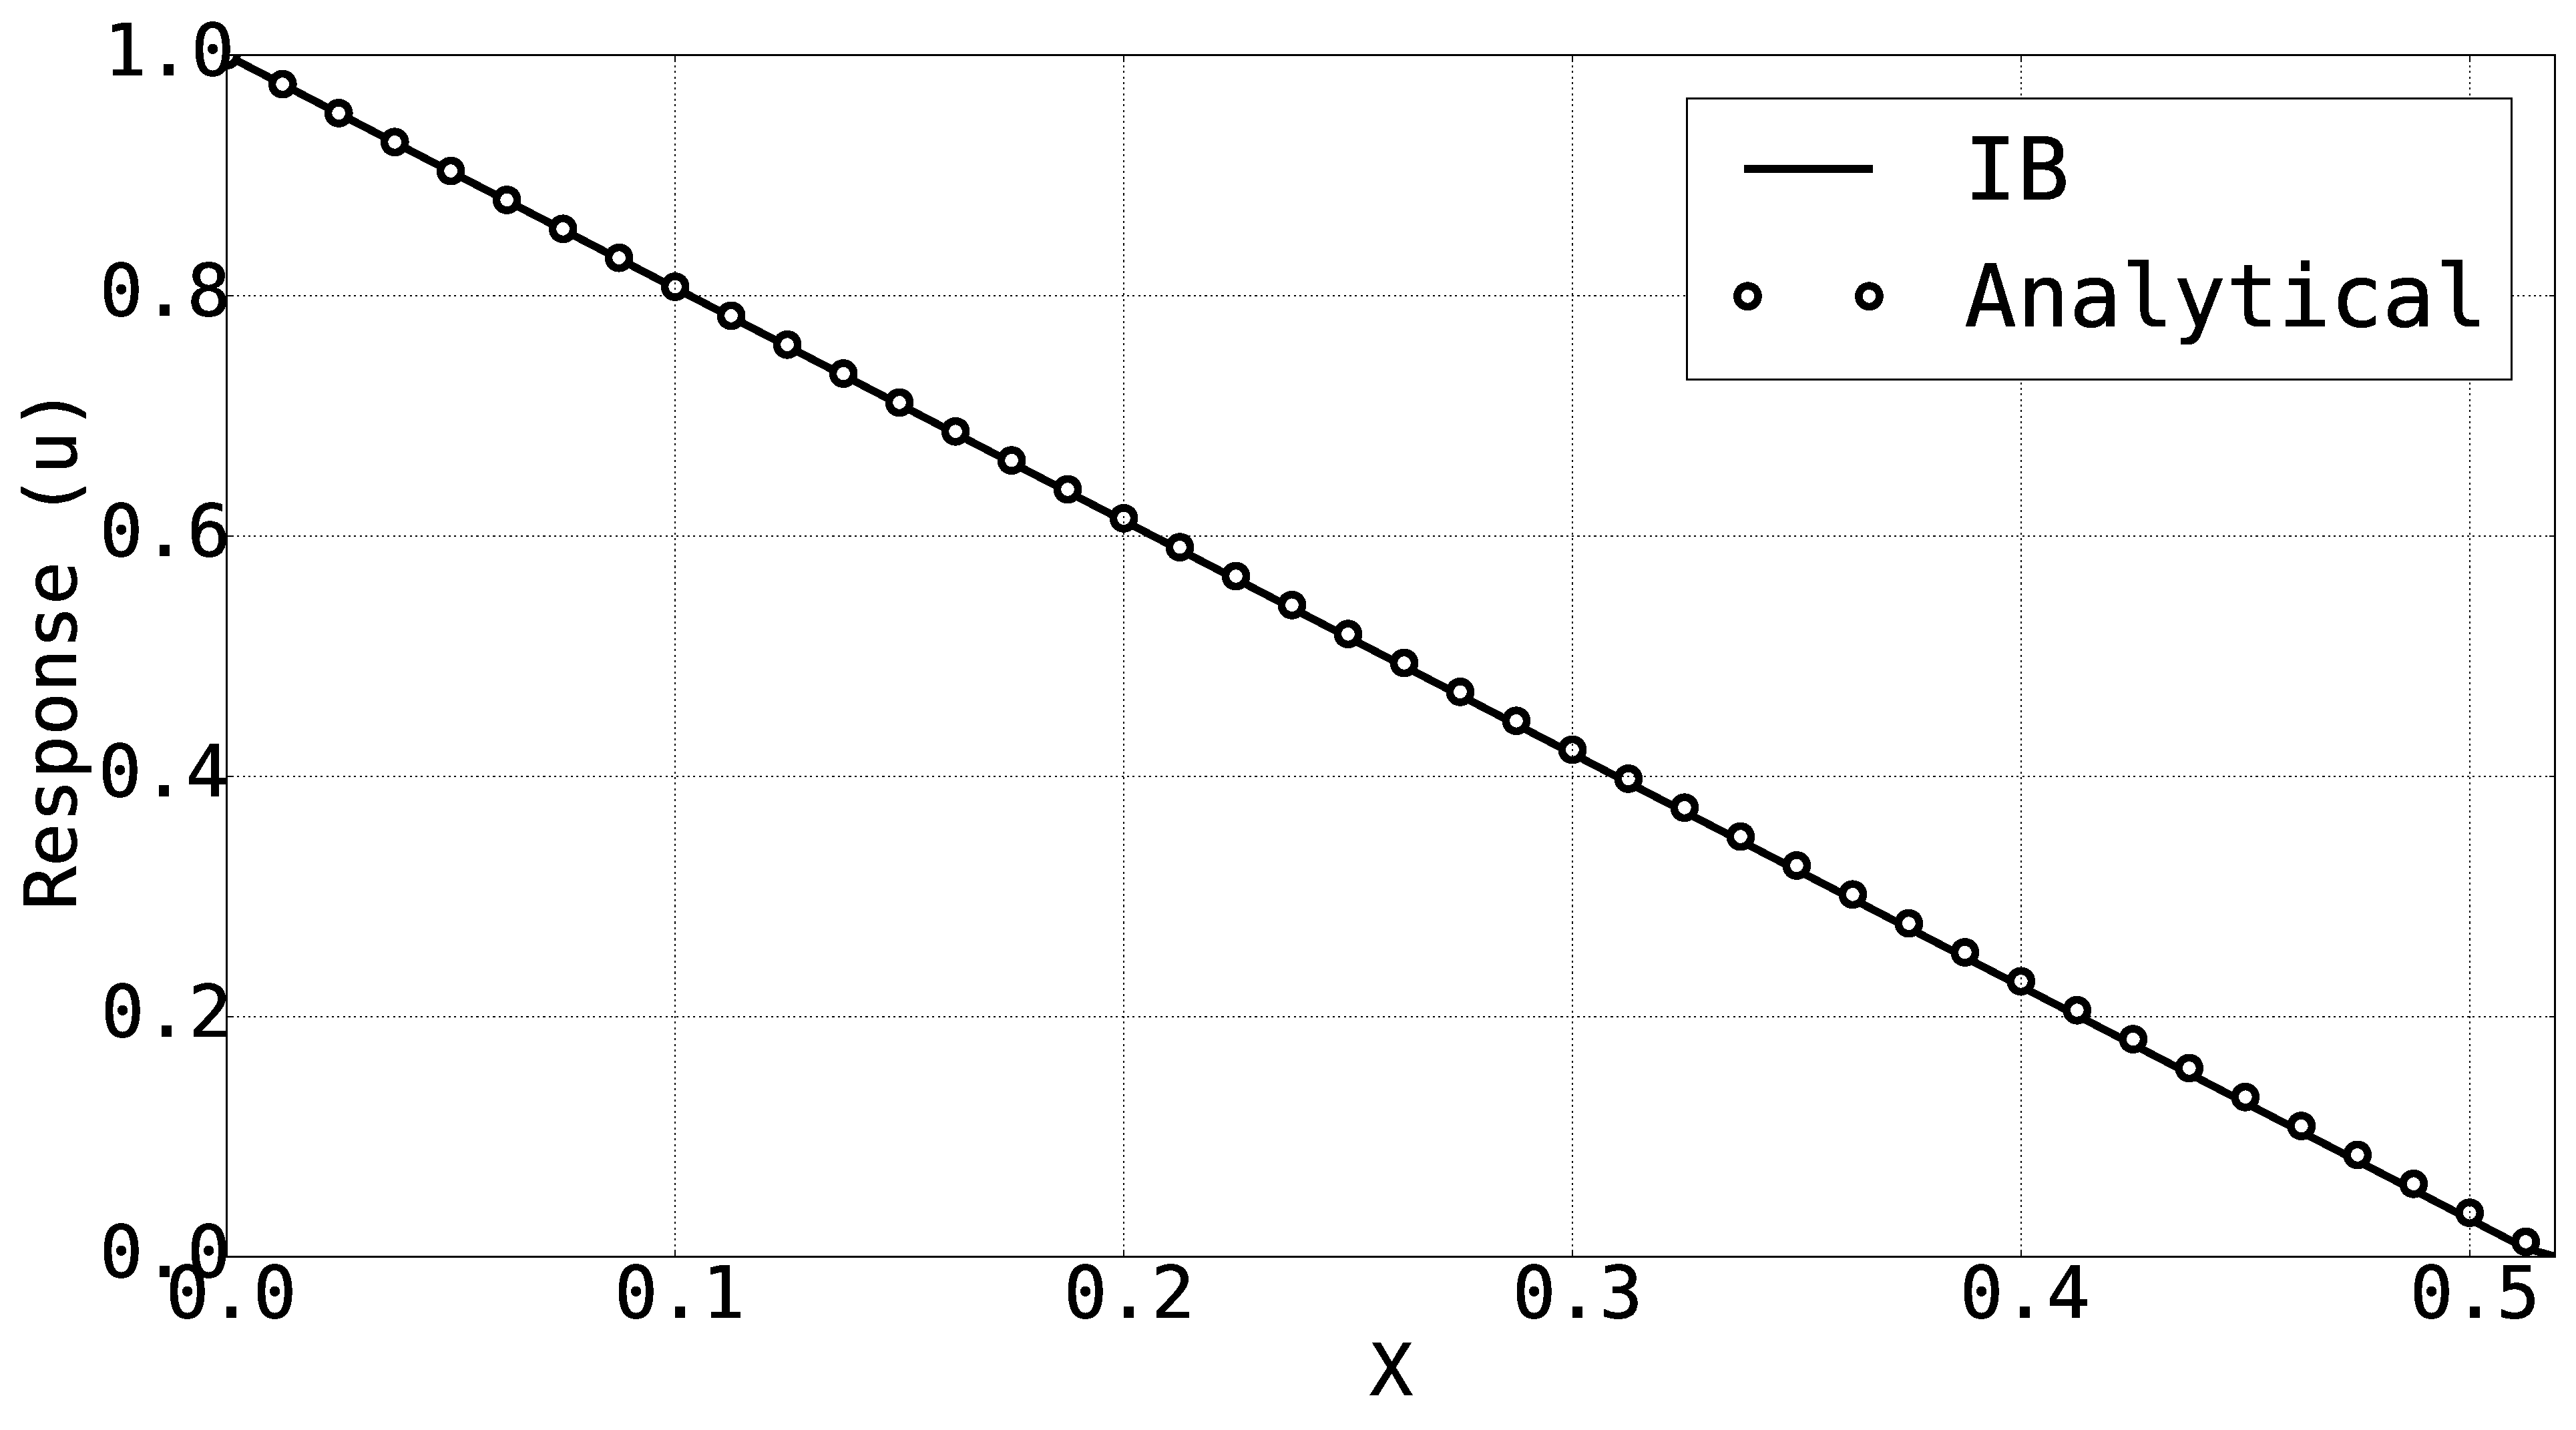
\includegraphics[width=7.0cm]{Chapter_3/figure/classicalIB_nodeNumber_4point_81.eps}
	}
	\\
	\subfigure[N = 161, 2-point delta function]
	{
	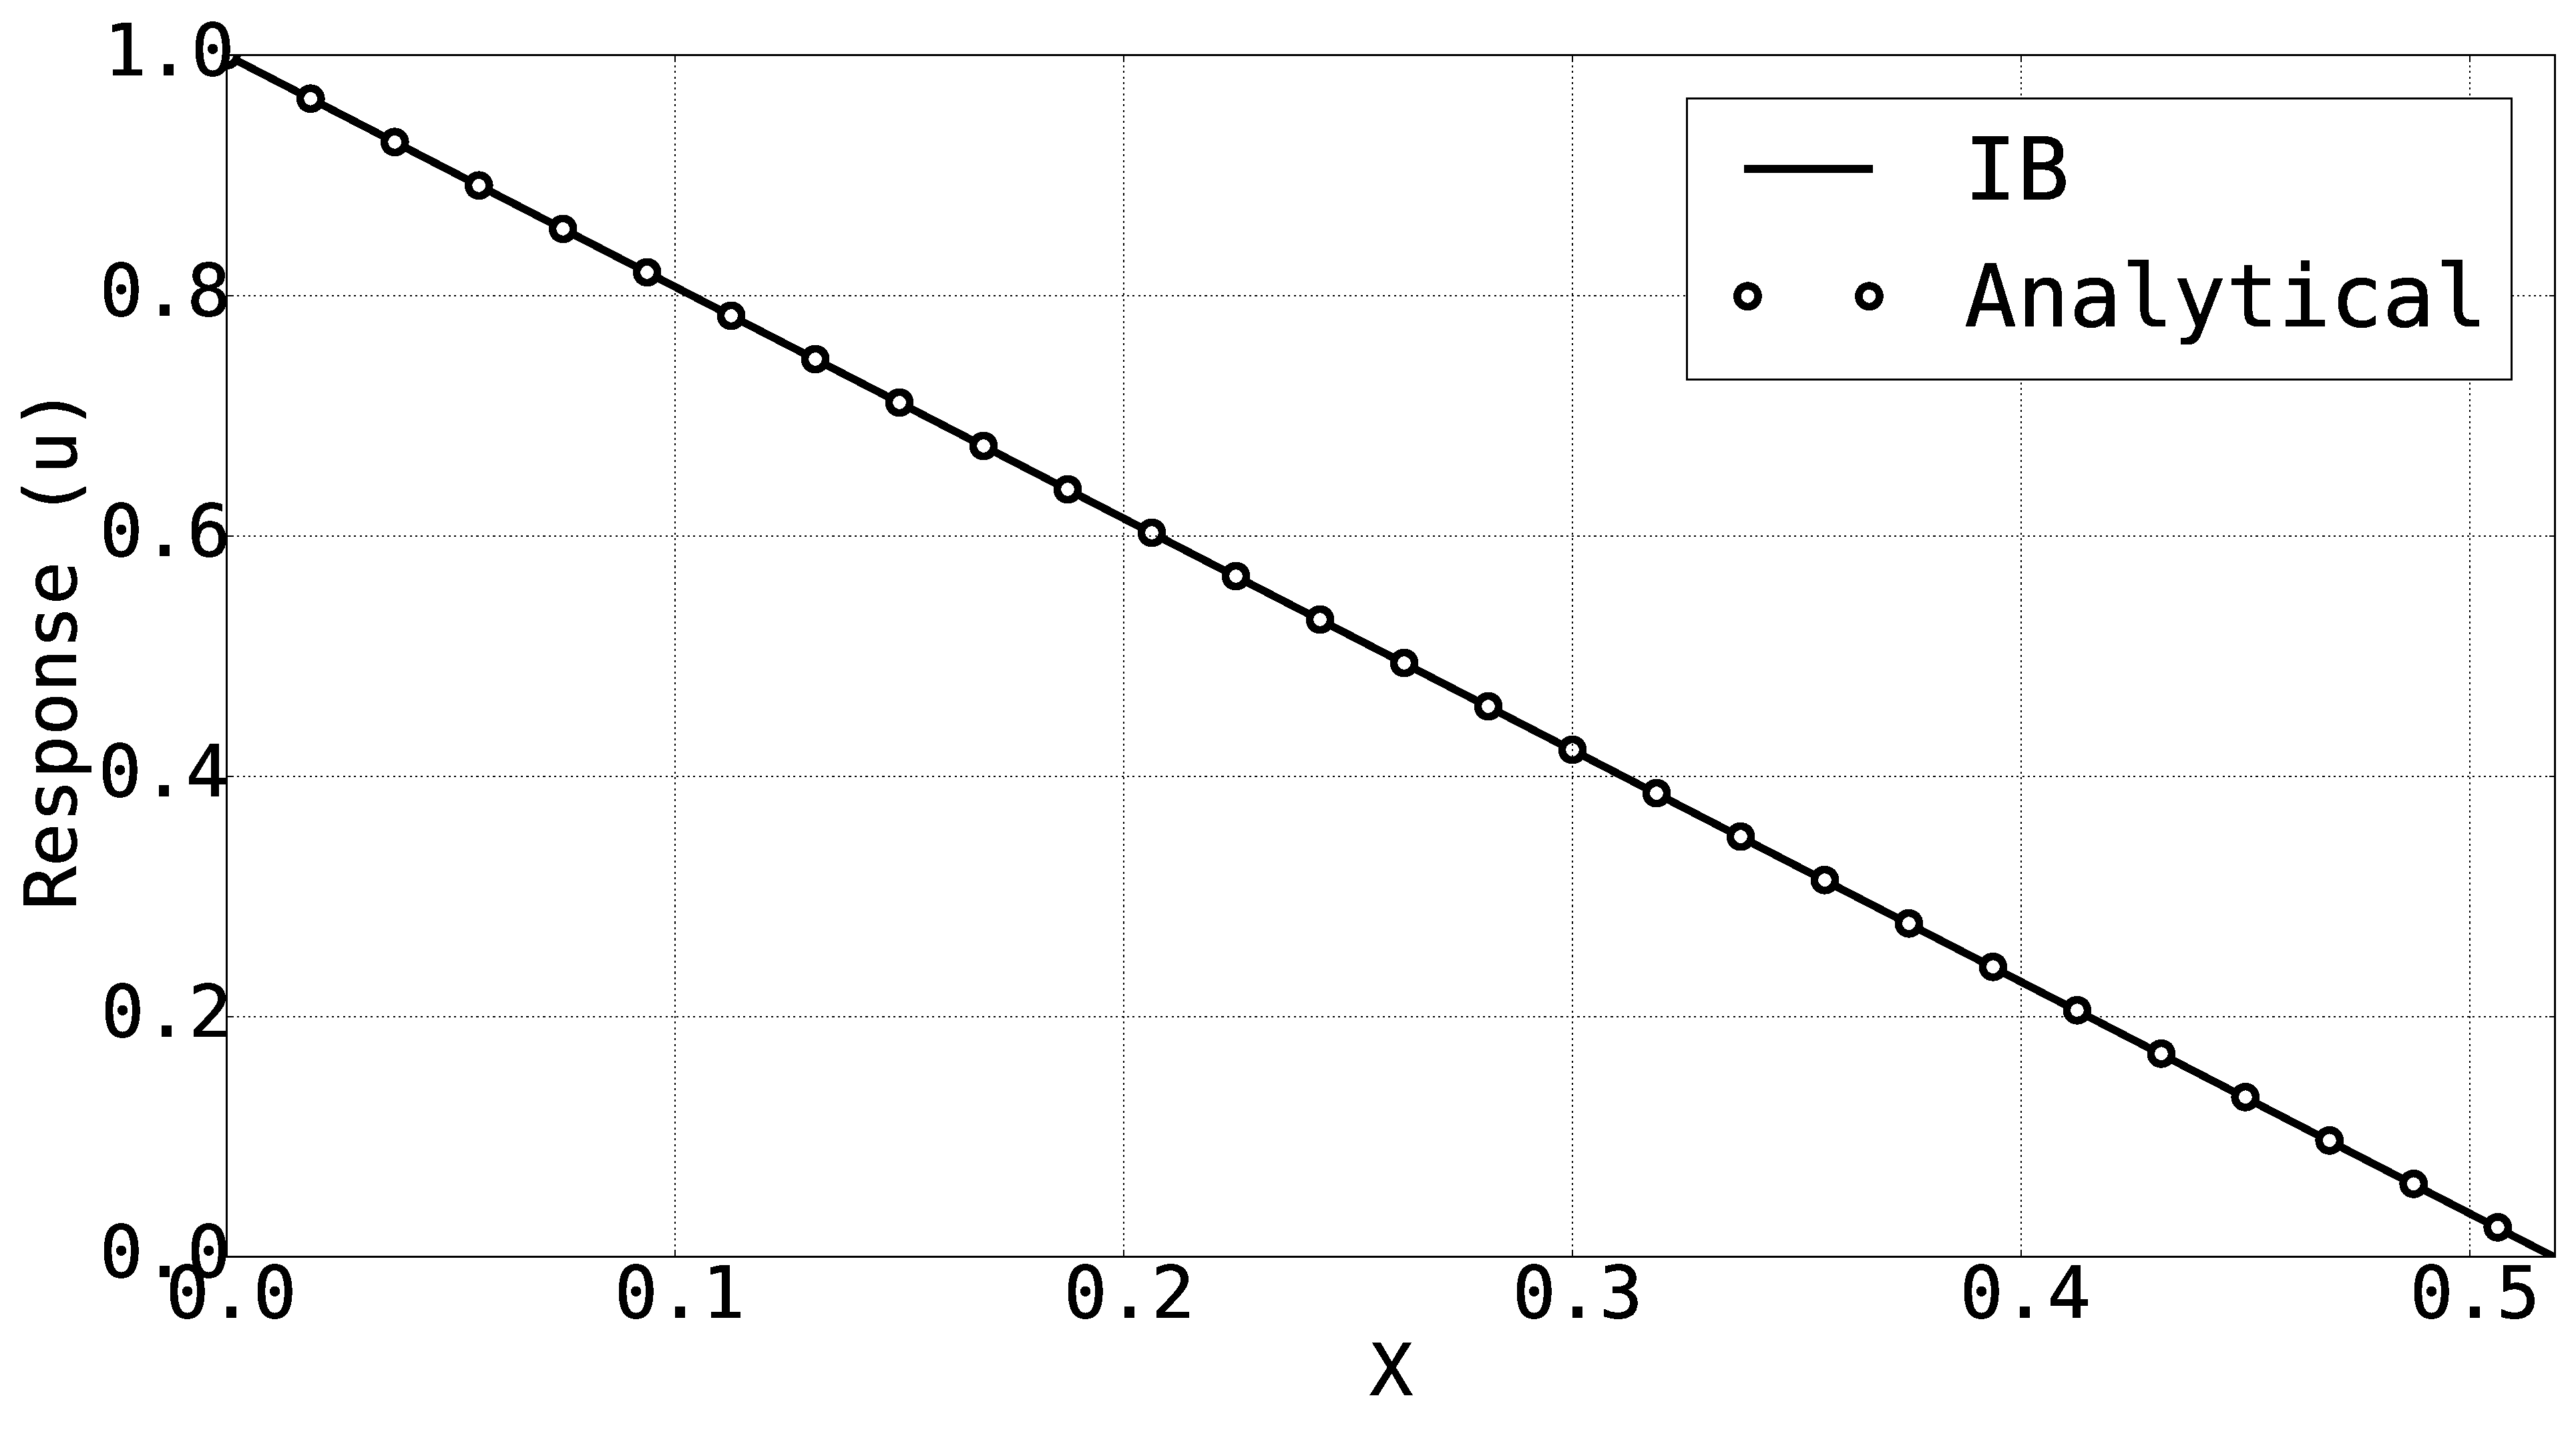
\includegraphics[width=7.0cm]{Chapter_3/figure/classicalIB_nodeNumber_2point_161.eps}
	}
	\quad
	\subfigure[N = 161, 4-point delta function]
	{
	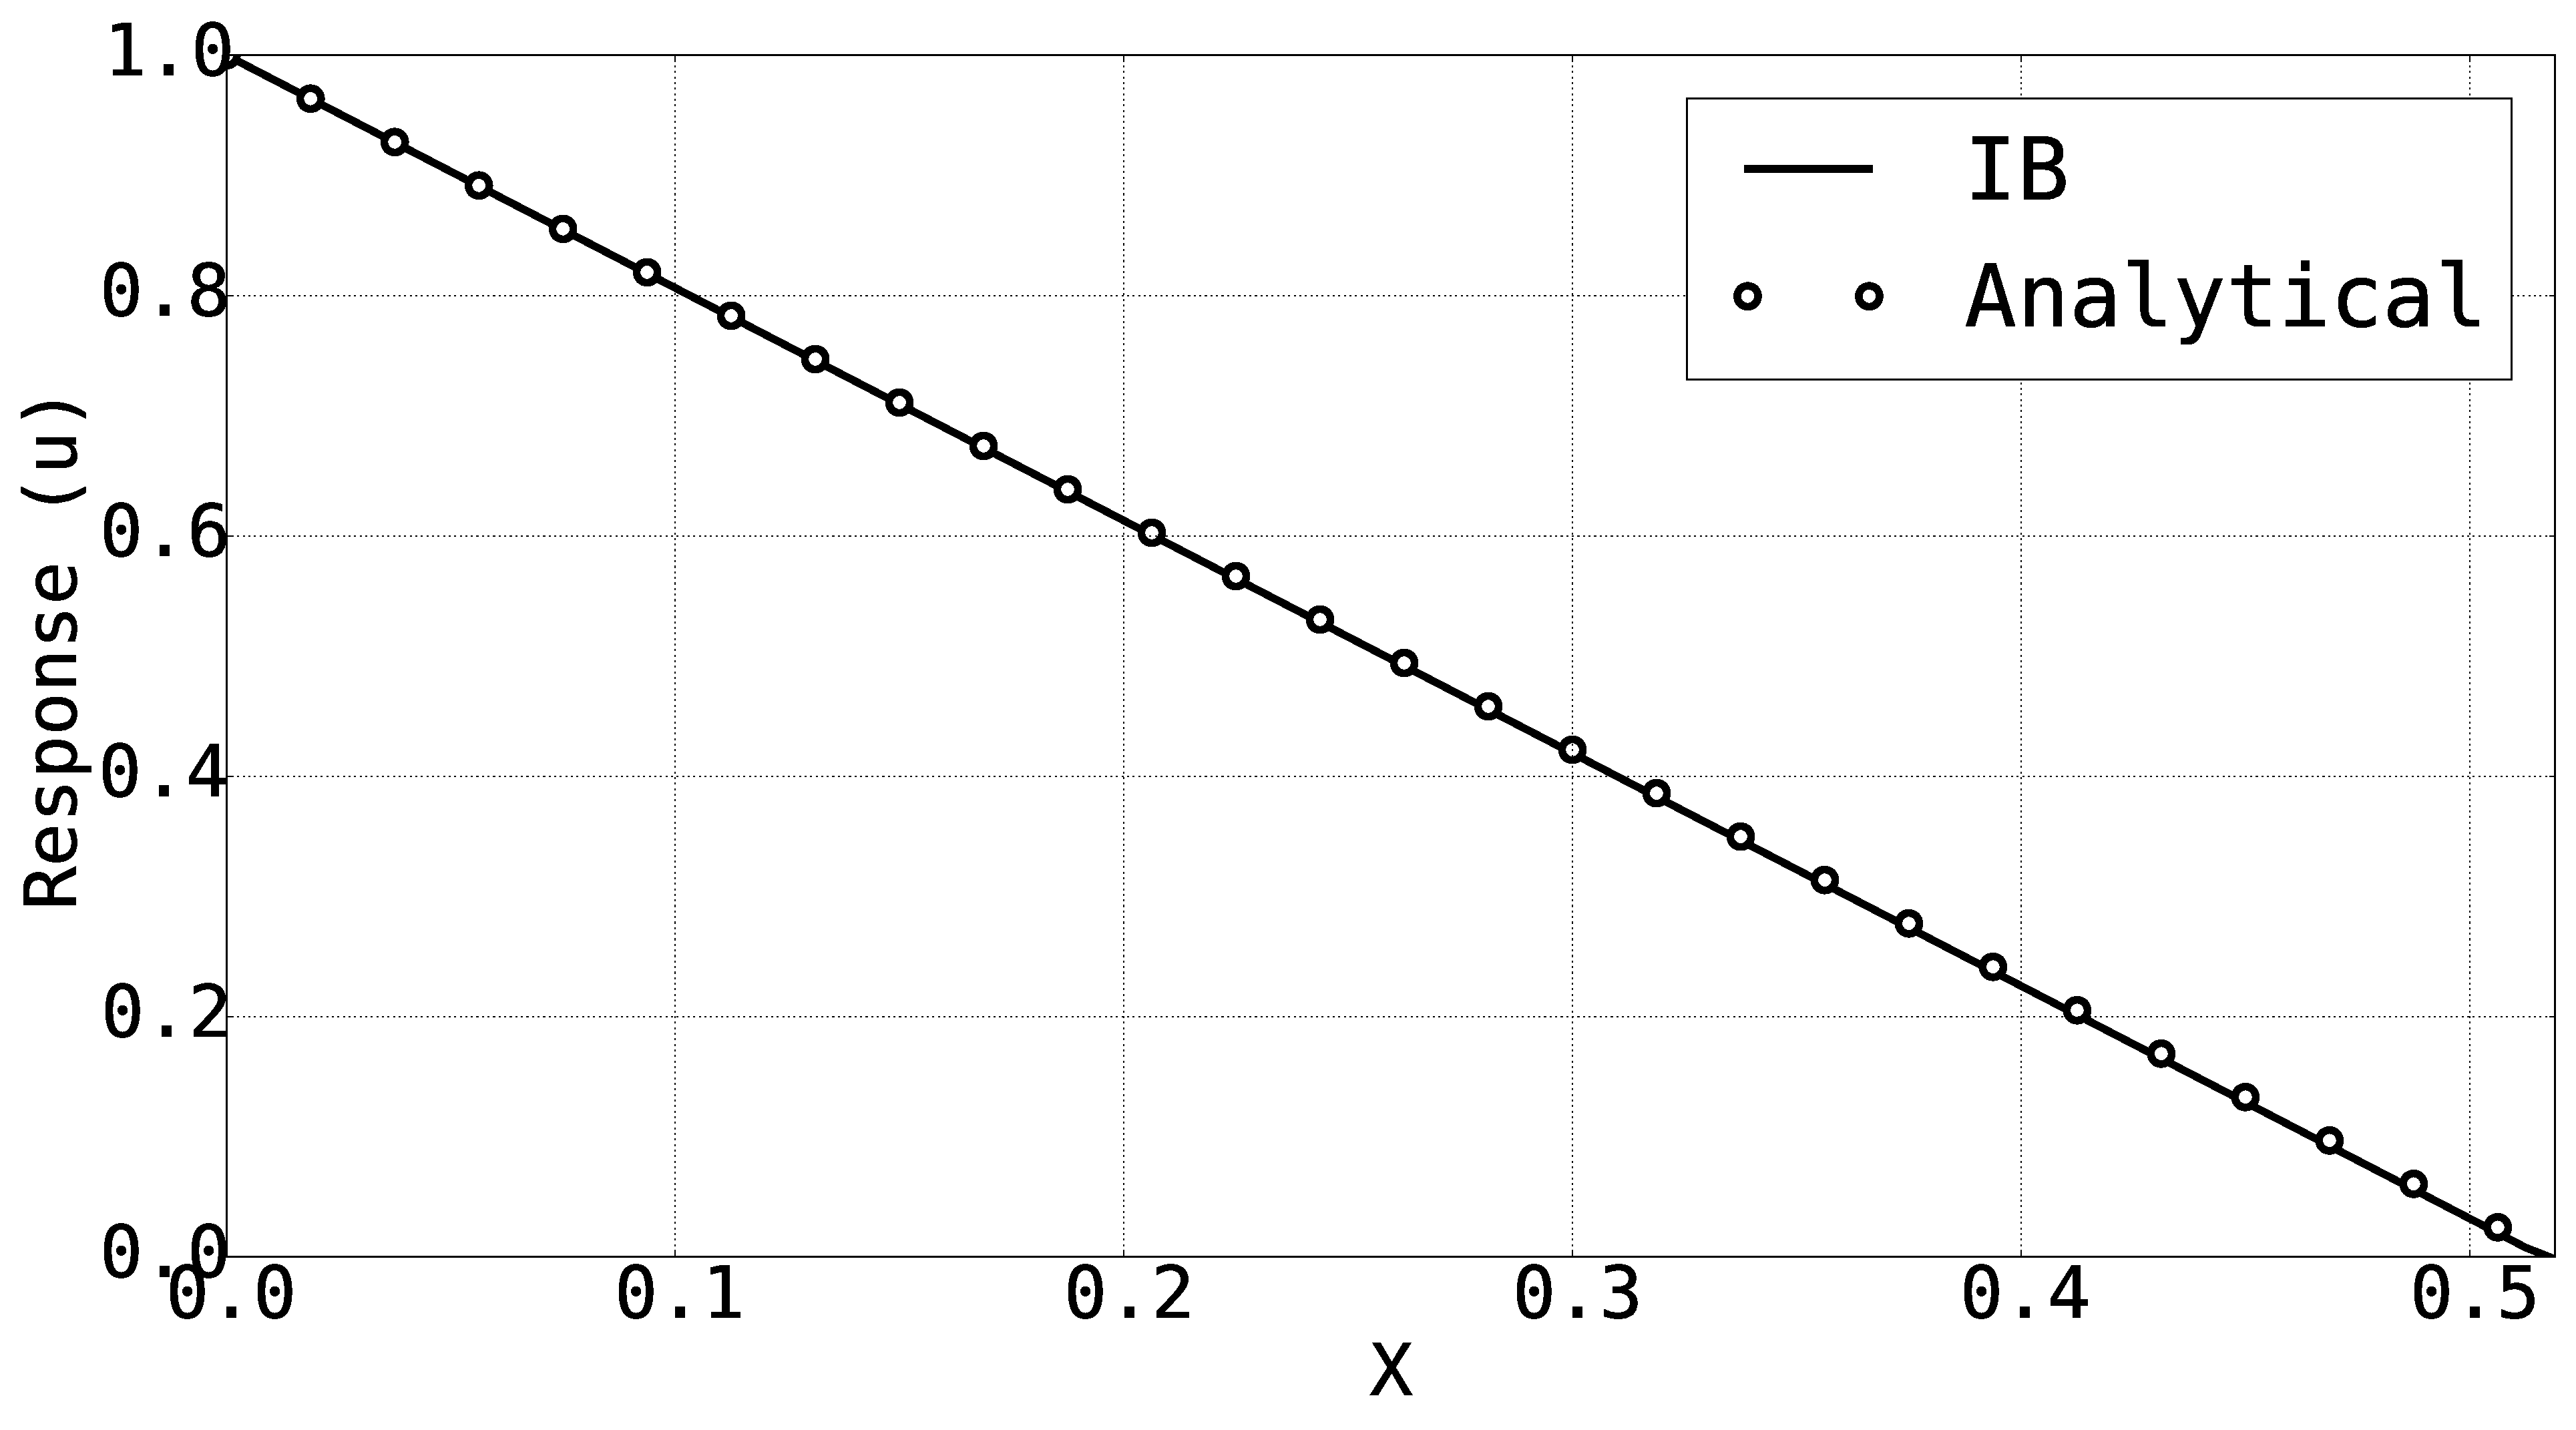
\includegraphics[width=7.0cm]{Chapter_3/figure/classicalIB_nodeNumber_4point_161.eps}
	}
	\caption{Comparison between IB and analytical results for different porosity values.}
	\label{fig:C3_classicalIBResultNodeNumber}
\end{figure}

\begin{table}[H]
\centering
\begin{tabular}{c | c | c}
	  & \multicolumn{2}{c}{RMSE value} \\ \hline
	 Node number & 2-point delta function & 4-point delta function \\ \hline \hline
	 11 & 0.0105 & 0.0292 \\ \hline
	 41 & 0.0035 & 0.002 \\ \hline
	 81 & 0.0026 & 0.0022 \\ \hline
	 161 & 0.00023 & 0.0002 \\
\end{tabular}
\caption{RMSE value for different node numbers and delta functions.}
\label{table:C3_classicalIBResultNodeNumberRMSE}
\end{table}

As shown in Figure \ref{fig:C3_classicalIBResultNodeNumber} and Table \ref{table:C3_classicalIBResultNodeNumberRMSE}, by increasing the number of nodes, the error in IB result decreases. However, changing the delta function from 2-point to 4-point does not effect the accuracy of the solution significantly. The higher order delta function can also decreases the accuracy of the solution for very low number of nodes (here 11). 

For the second investigation, we looked at the effect of changing the moving wall velocity on the solution accuracy. For this simulation, we fixed the number of nodes to 81 and set the stiffness value to $10^2$. The wall location is fixed at $0.51885$. The time step is also chosen as $10^{-5}$. For this problem, we only focused on 2-point delta function. We chose the wall velocity as $10$, $10^2$, $10^3$, and $10^4$. As shown in Figure \ref{fig:C3_classicalIBResultWallVelocity} and Table \ref{fig:C3_classicalIBResultWallVelocityRMSE}, the method is capable of handling flow with different velocity without a loss in accuracy of the results. However, the simulation time increases with increase in wall velocity.

\begin{figure}[H]
	\centering
	\subfigure[$u_{wall} = 10 m/s$]
	{
	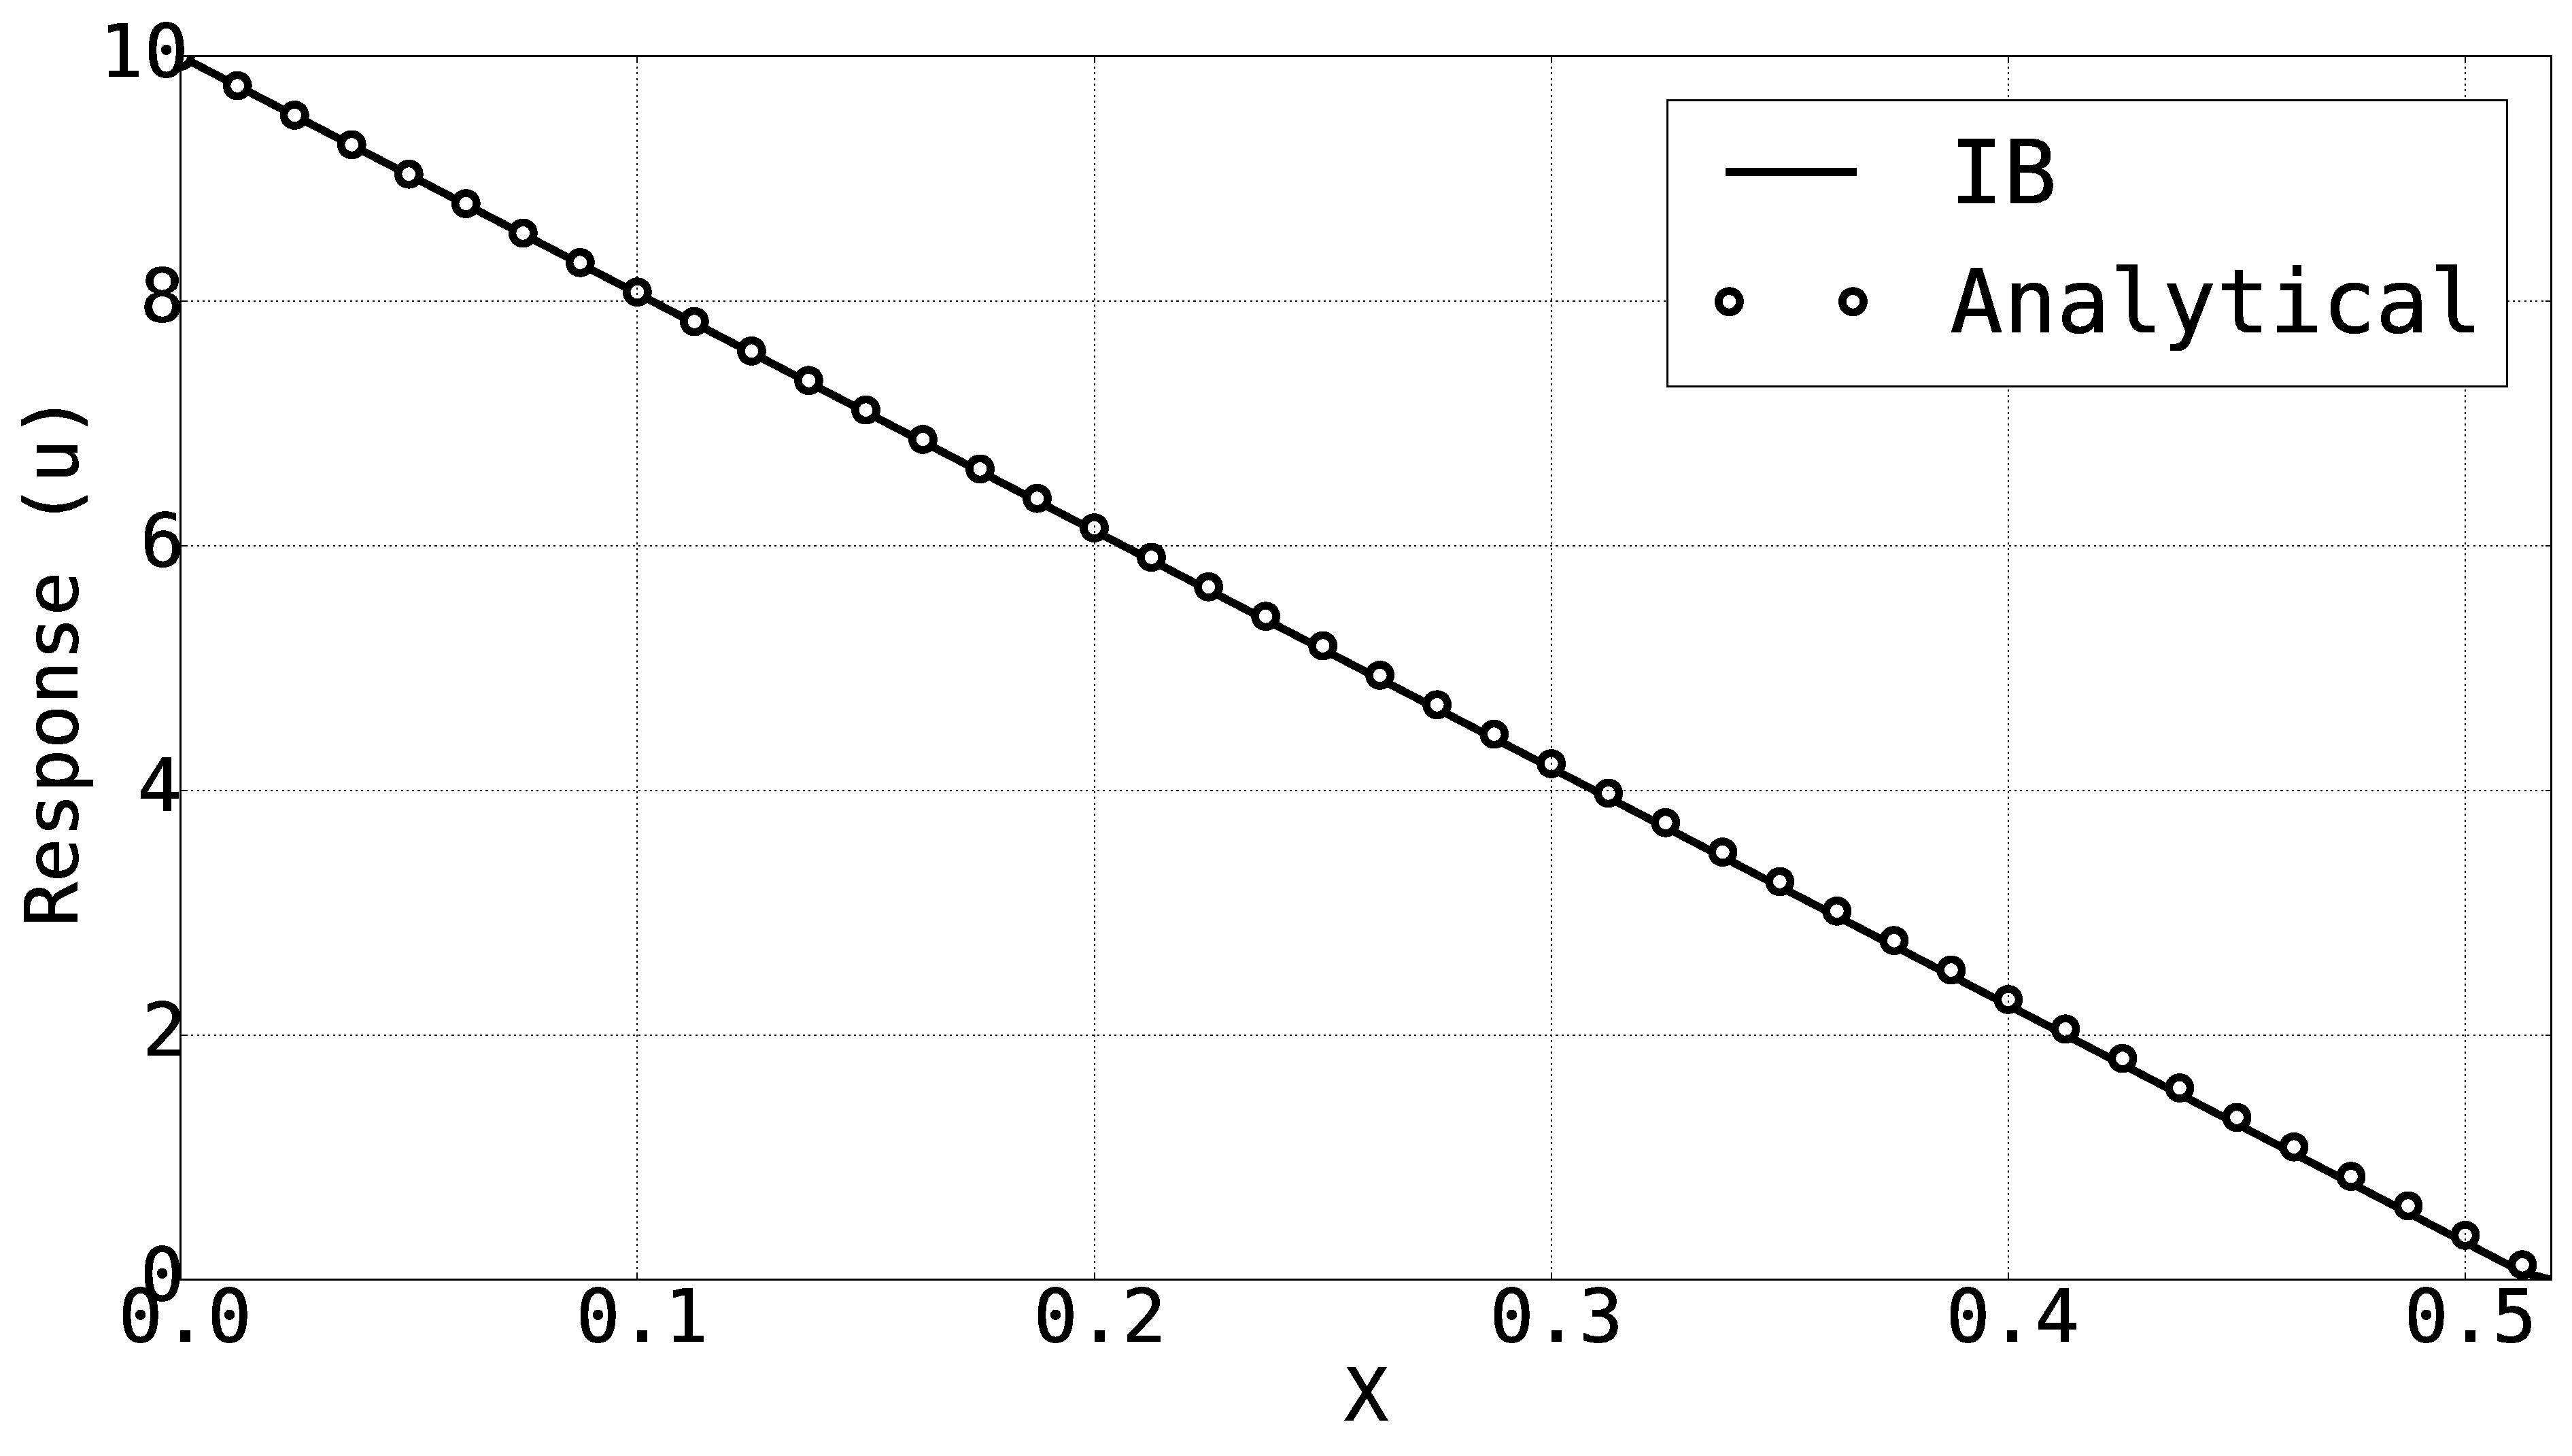
\includegraphics[width=7.0cm]{Chapter_3/figure/classicalIB_wallVelocity_2point_10.eps}
	}
	\quad
	\subfigure[$u_{wall} = 10^2 m/s$]
	{
	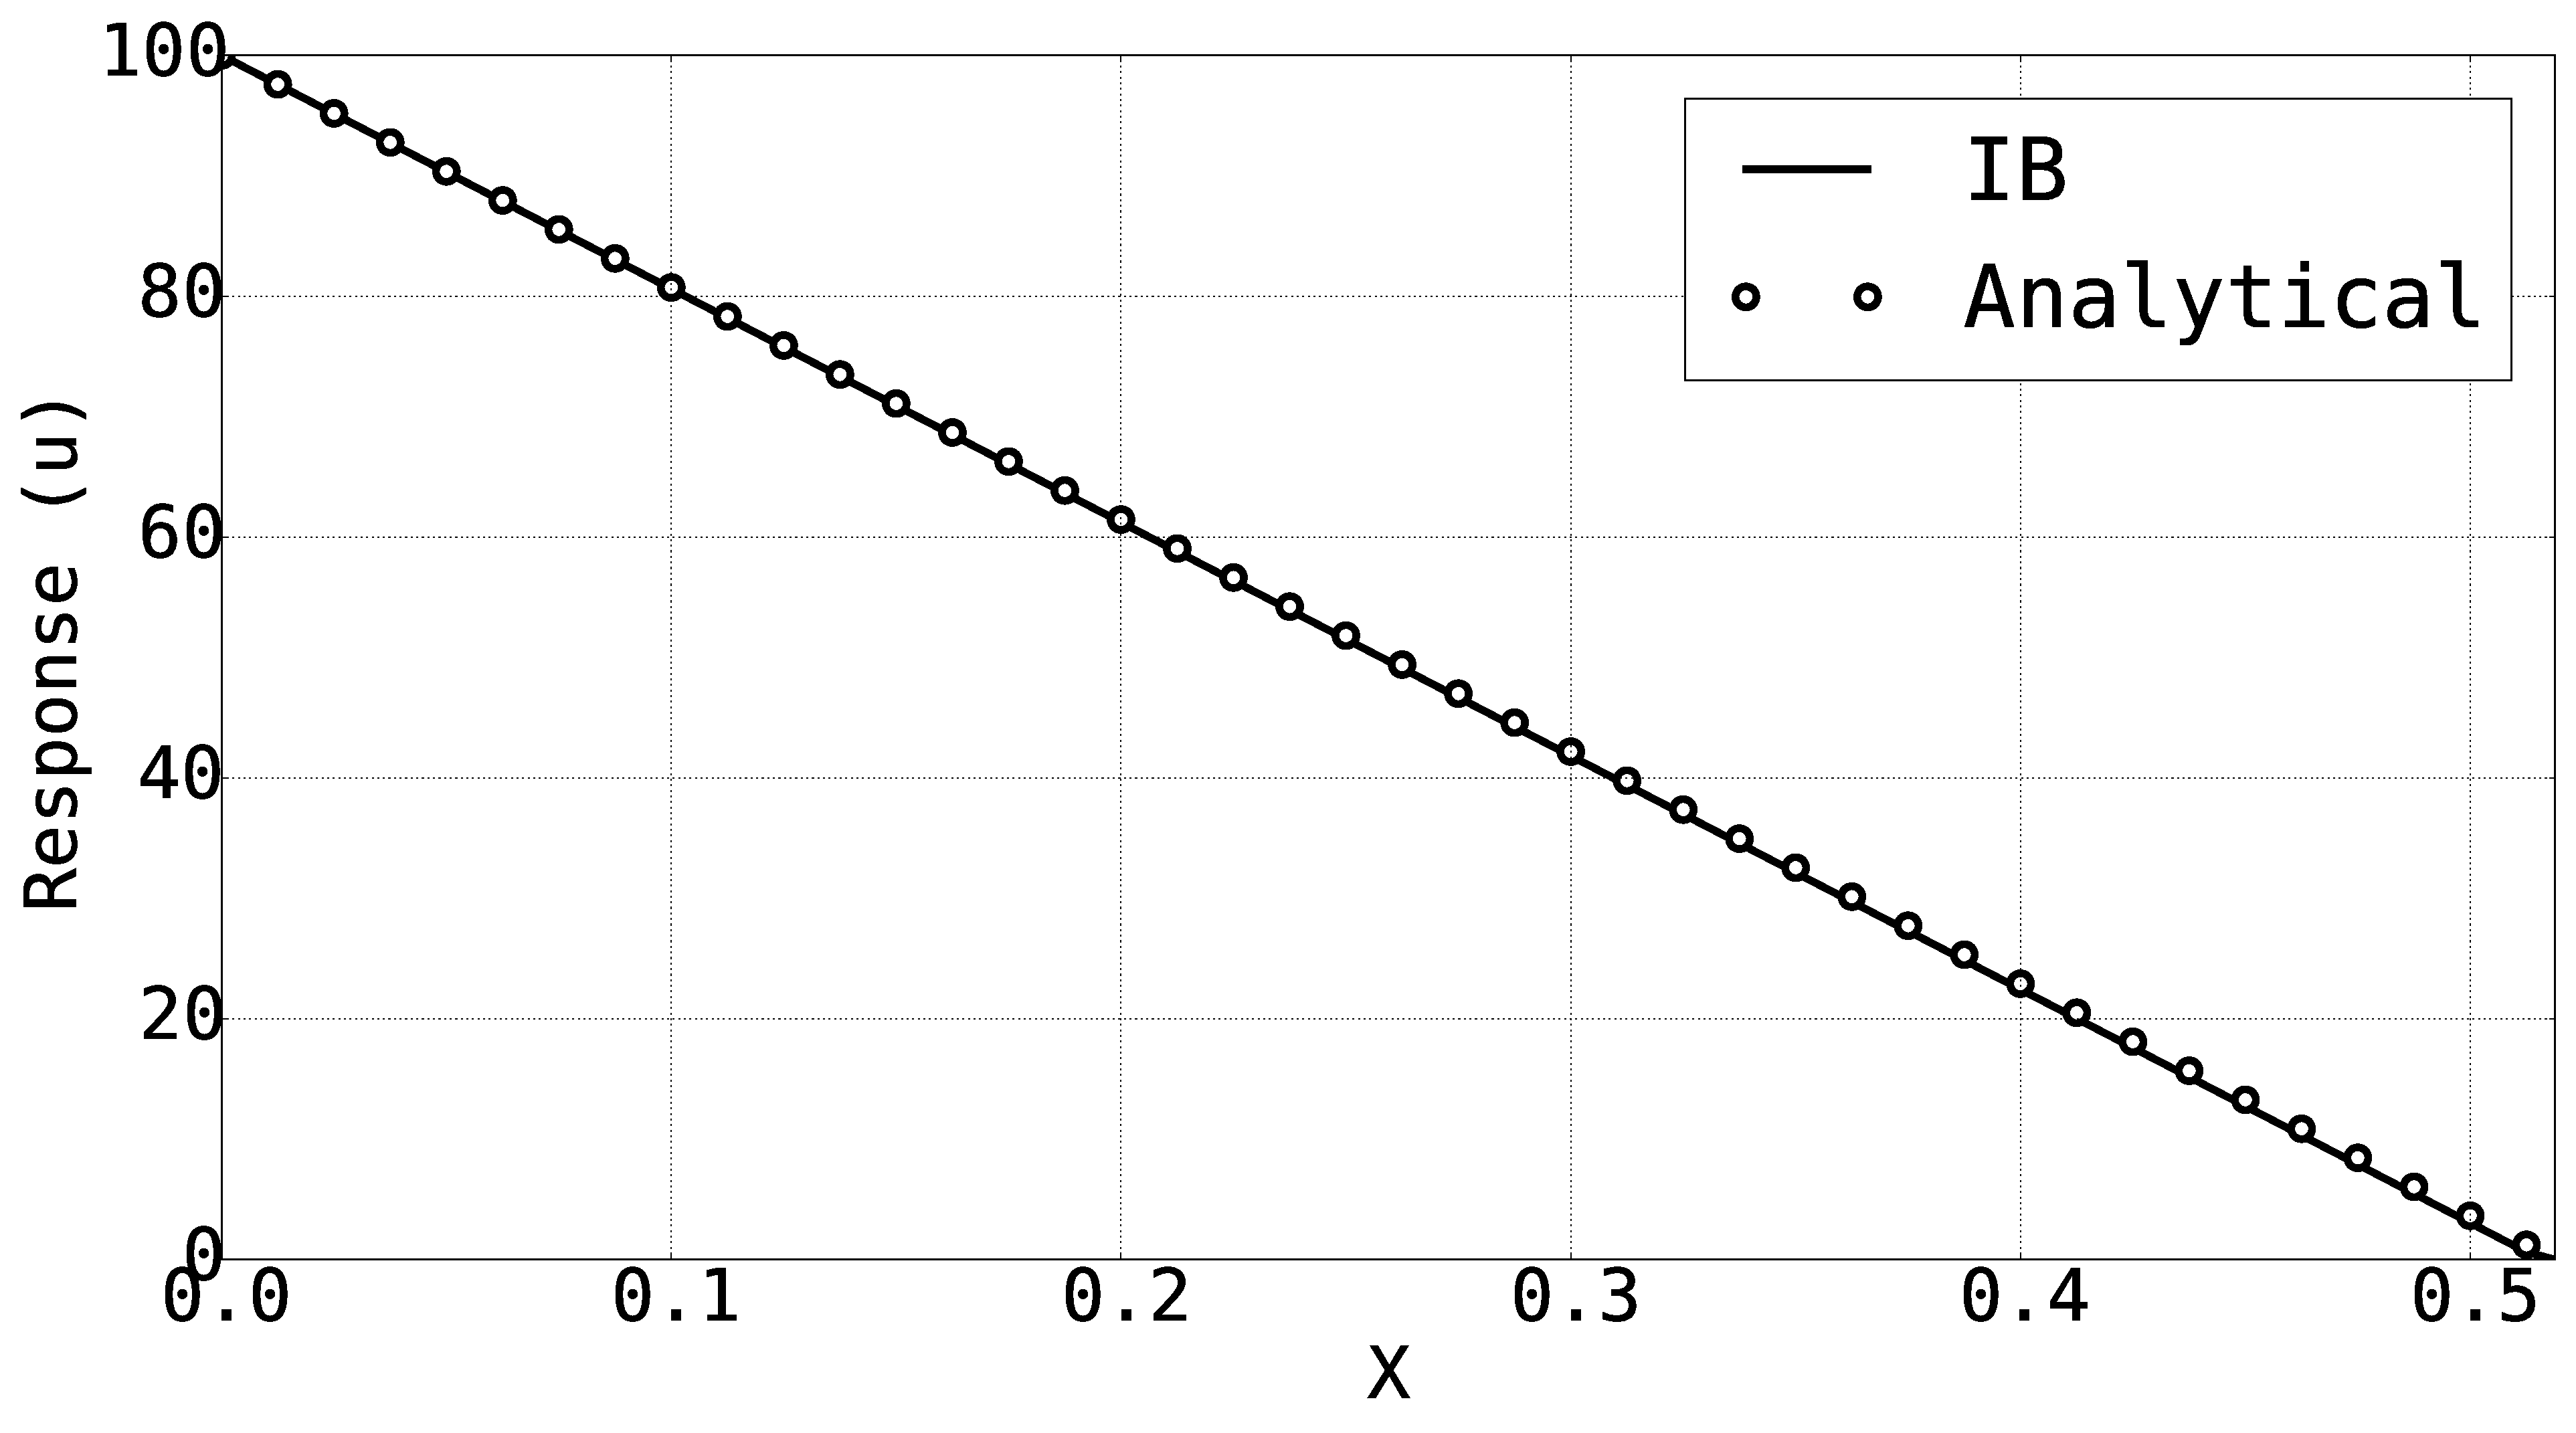
\includegraphics[width=7.0cm]{Chapter_3/figure/classicalIB_wallVelocity_2point_100.eps}
	}
	\\
	\subfigure[$u_{wall} = 10^3 m/s$]
	{
	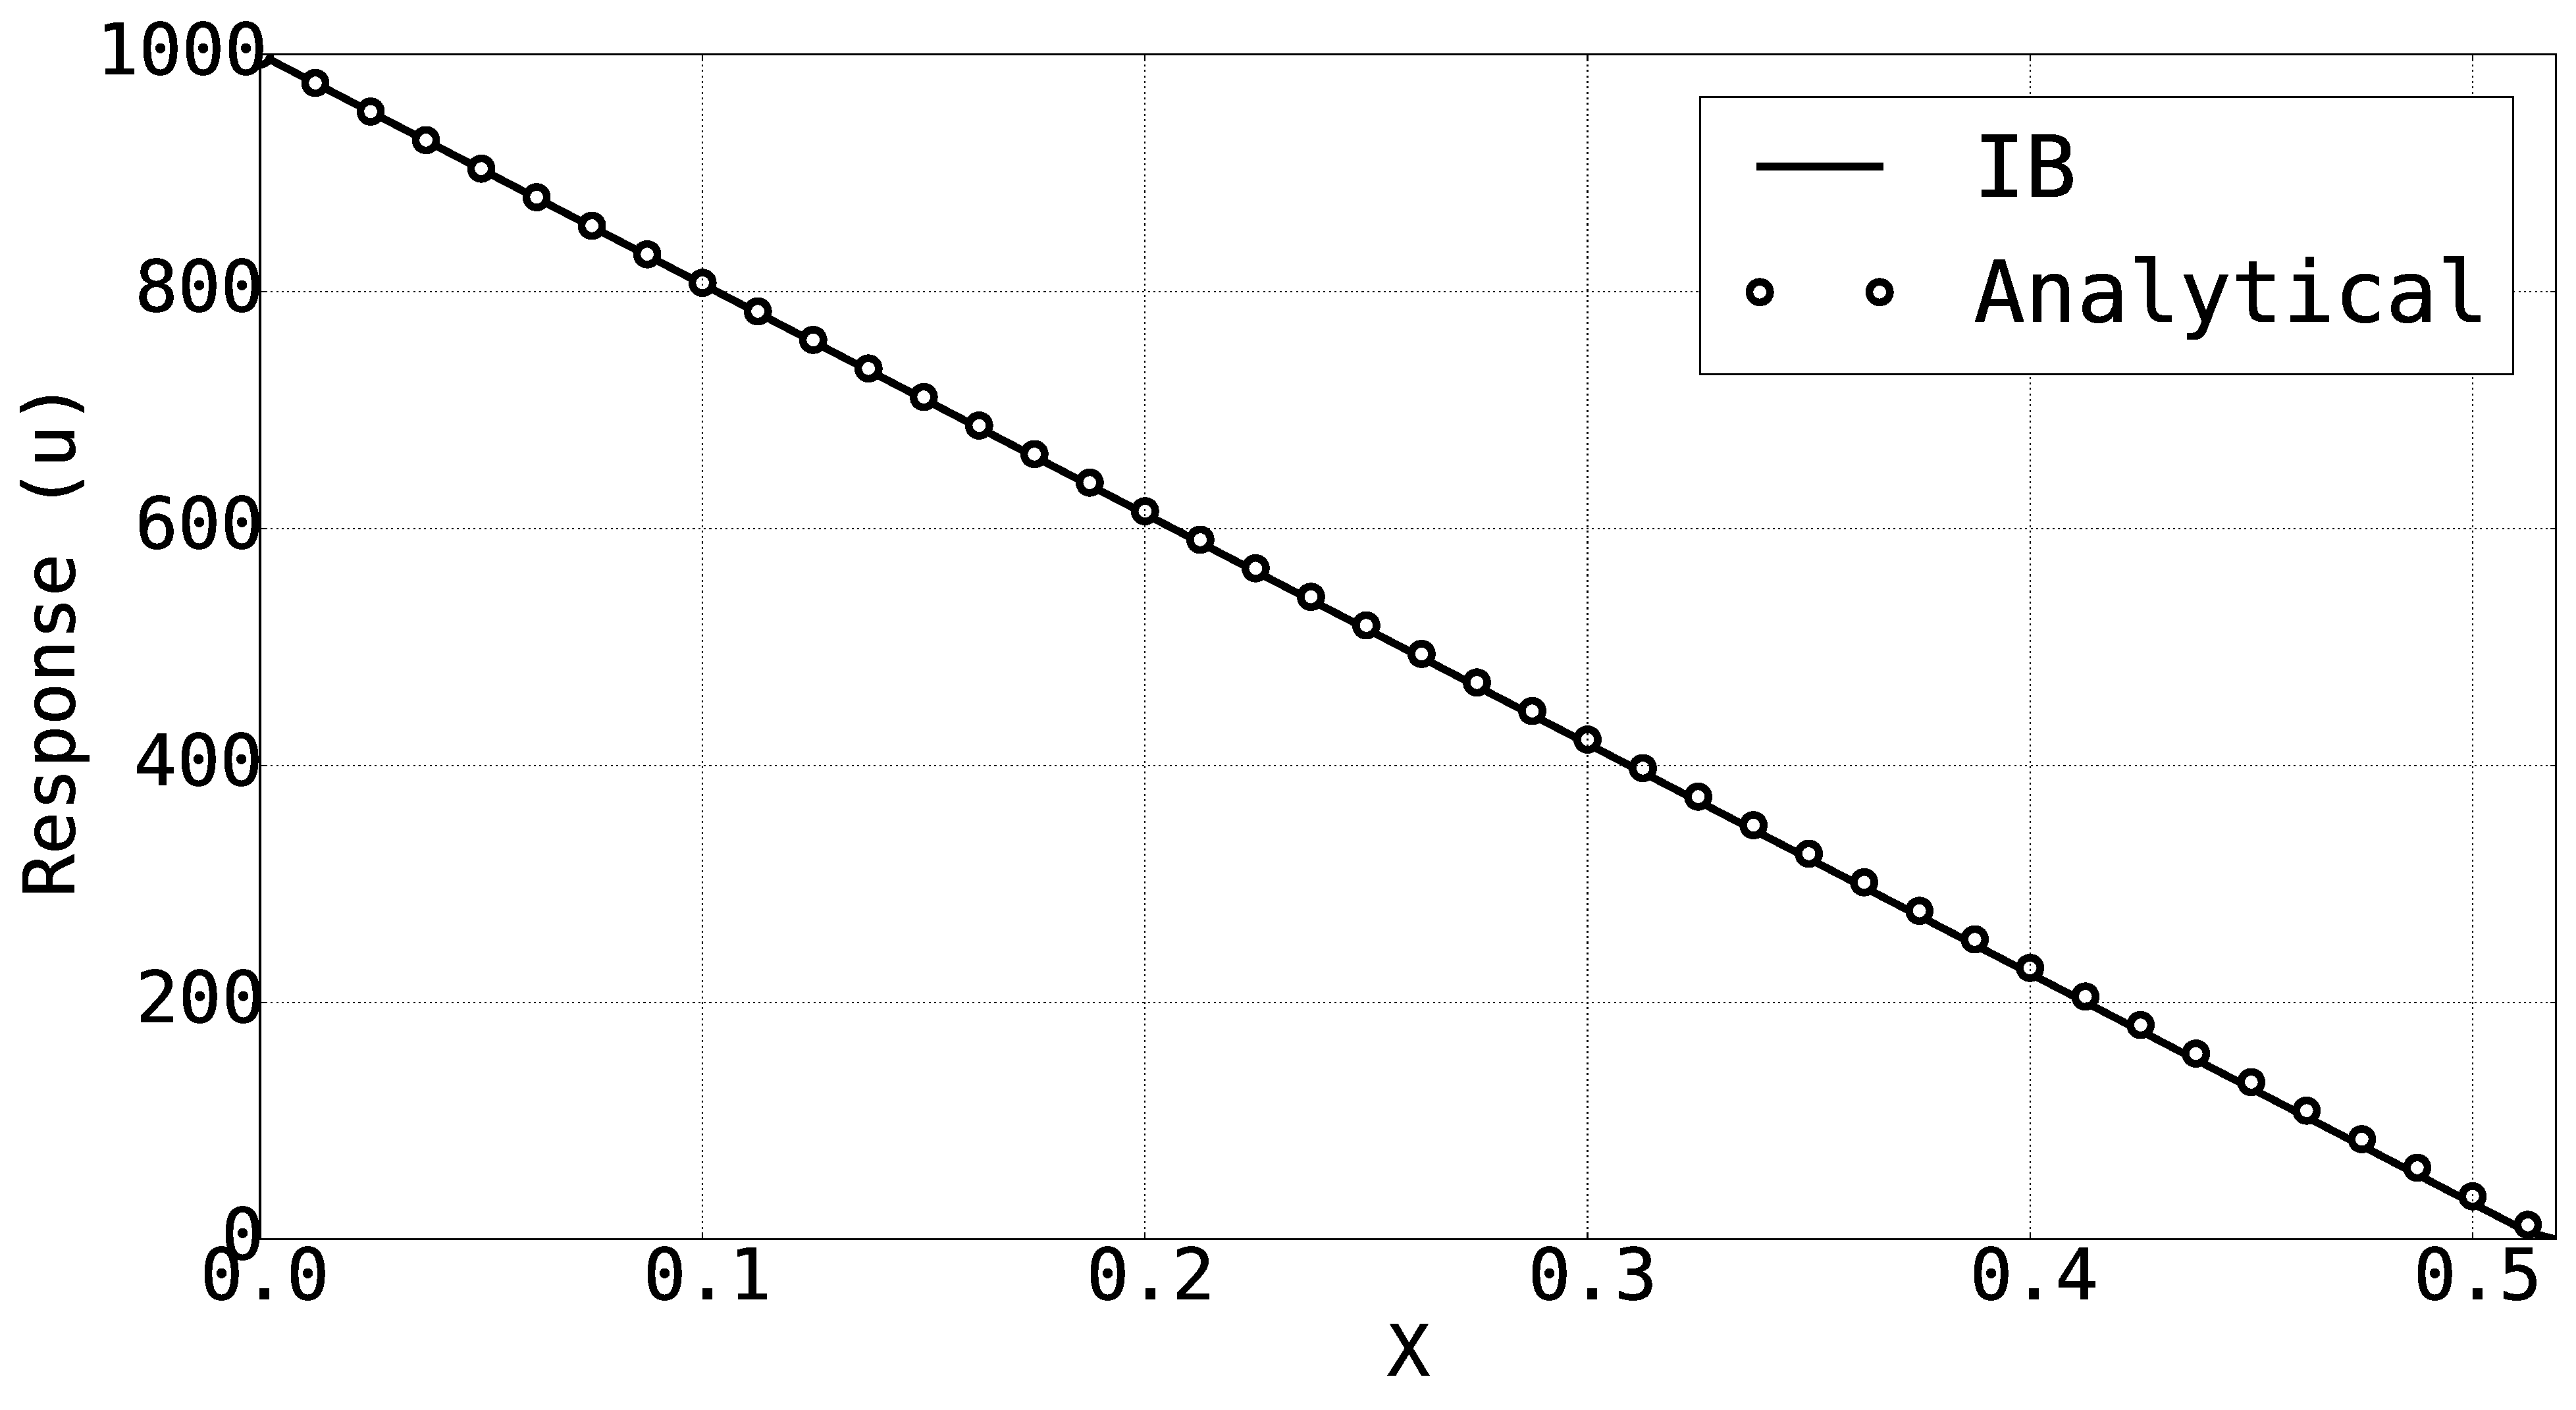
\includegraphics[width=7.0cm]{Chapter_3/figure/classicalIB_wallVelocity_2point_1000.eps}
	}
	\quad
	\subfigure[$u_{wall} = 10^4 m/s$]
	{
	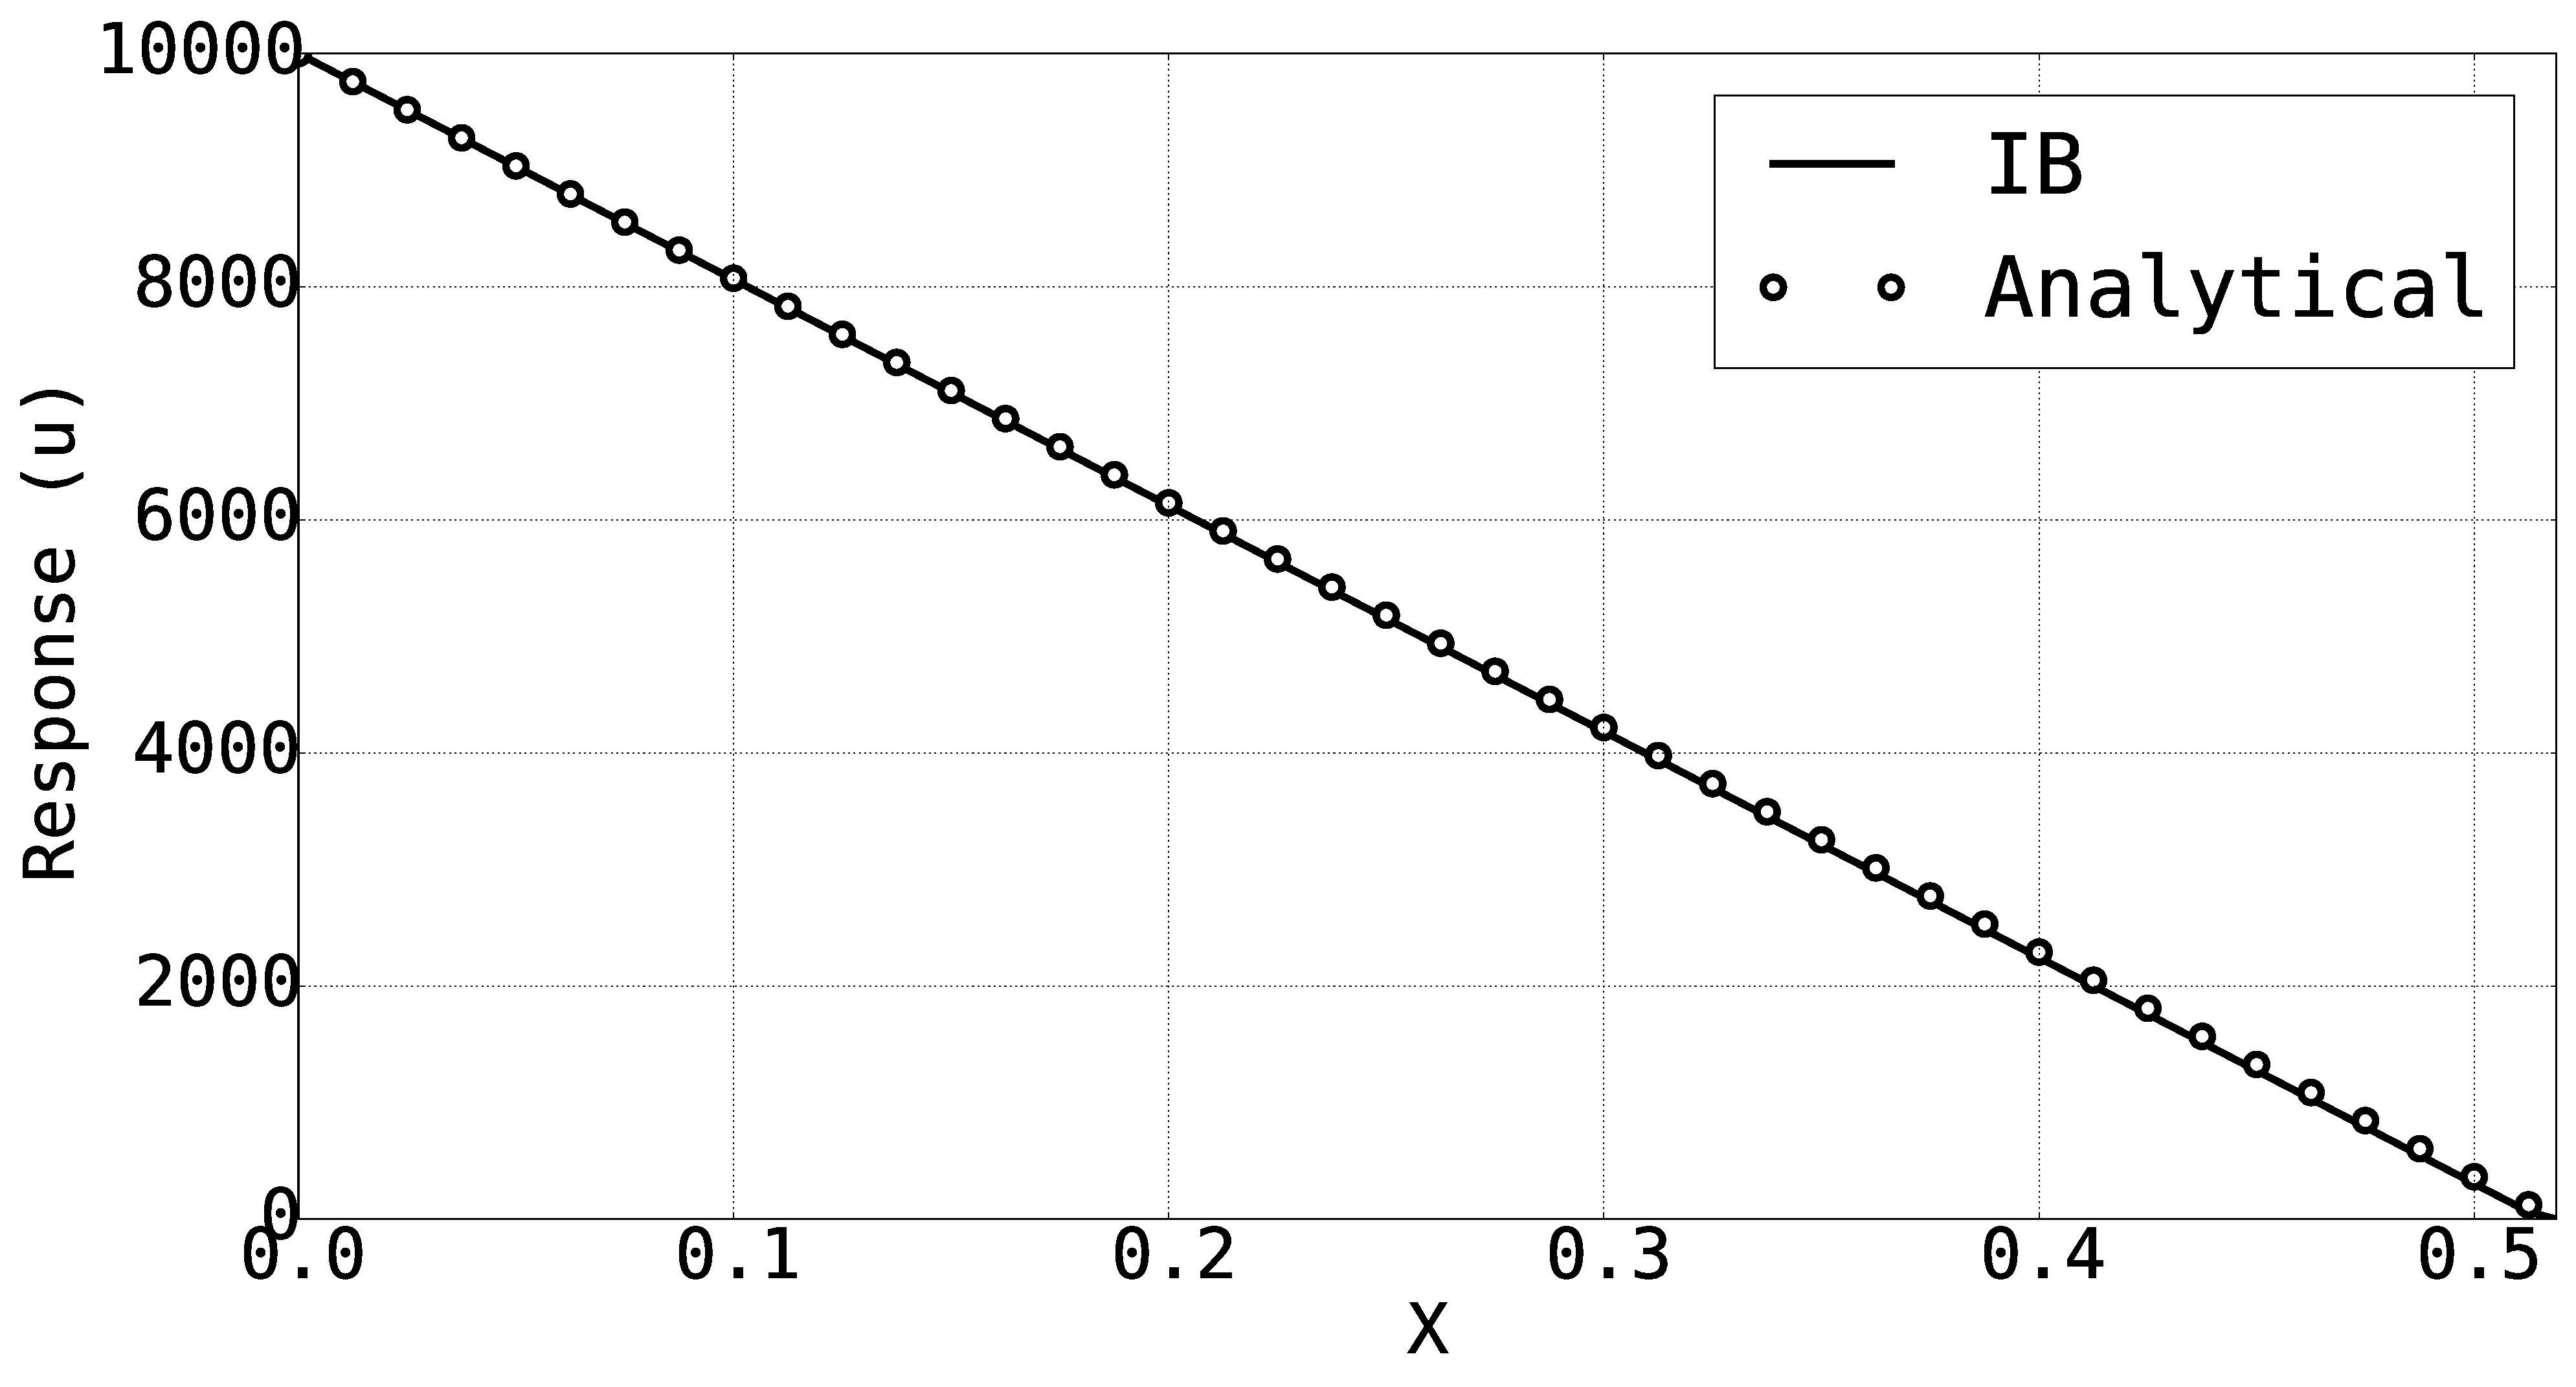
\includegraphics[width=7.0cm]{Chapter_3/figure/classicalIB_wallVelocity_2point_10000.eps}
	}
	\caption{Comparison between IB and analytical results for different wall velocities.}
	\label{fig:C3_classicalIBResultWallVelocity}
\end{figure}

\begin{table}[H]
\centering
\begin{tabular}{c | c}
	 Wall velocity & RMSE \\ \hline \hline
	 10 & 0.0024\\ \hline
	 $10^2$ & 0.0024 \\ \hline
	 $10^3$ & 0.0024 \\ \hline
	 $10^4$ & 0.0024 \\
\end{tabular}
\caption{RMSE value for different wall velocities.}
\label{table:C3_classicalIBResultWallVelocityRMSE}
\end{table}

For the last case study of classical IB method, we looked at the effect of the wall stiffness on the accuracy of the solution. For this case, we fixed the wall location at $x_{wall} = 0.51885$ and defined the wall velocity as $10 m/s$. The time step is selected as $10^{-5}$. We looked at the wall stiffness of $0.1$, $1$, $10$, and $100$. As shown in Figure \ref{fig:C3_classicalIBResultWallStiffness} and Table \ref{table:C3_classicalIBResultWallStiffnessRMSE}, wall stiffness has a considerable effect of the solution result. Therefore, a convergence study for the wall stiffness value is usually required if one wants to model the stiff boundaries.

\begin{figure}[H]
	\centering
	\subfigure[$K_{wall} = 0.1$]
	{
	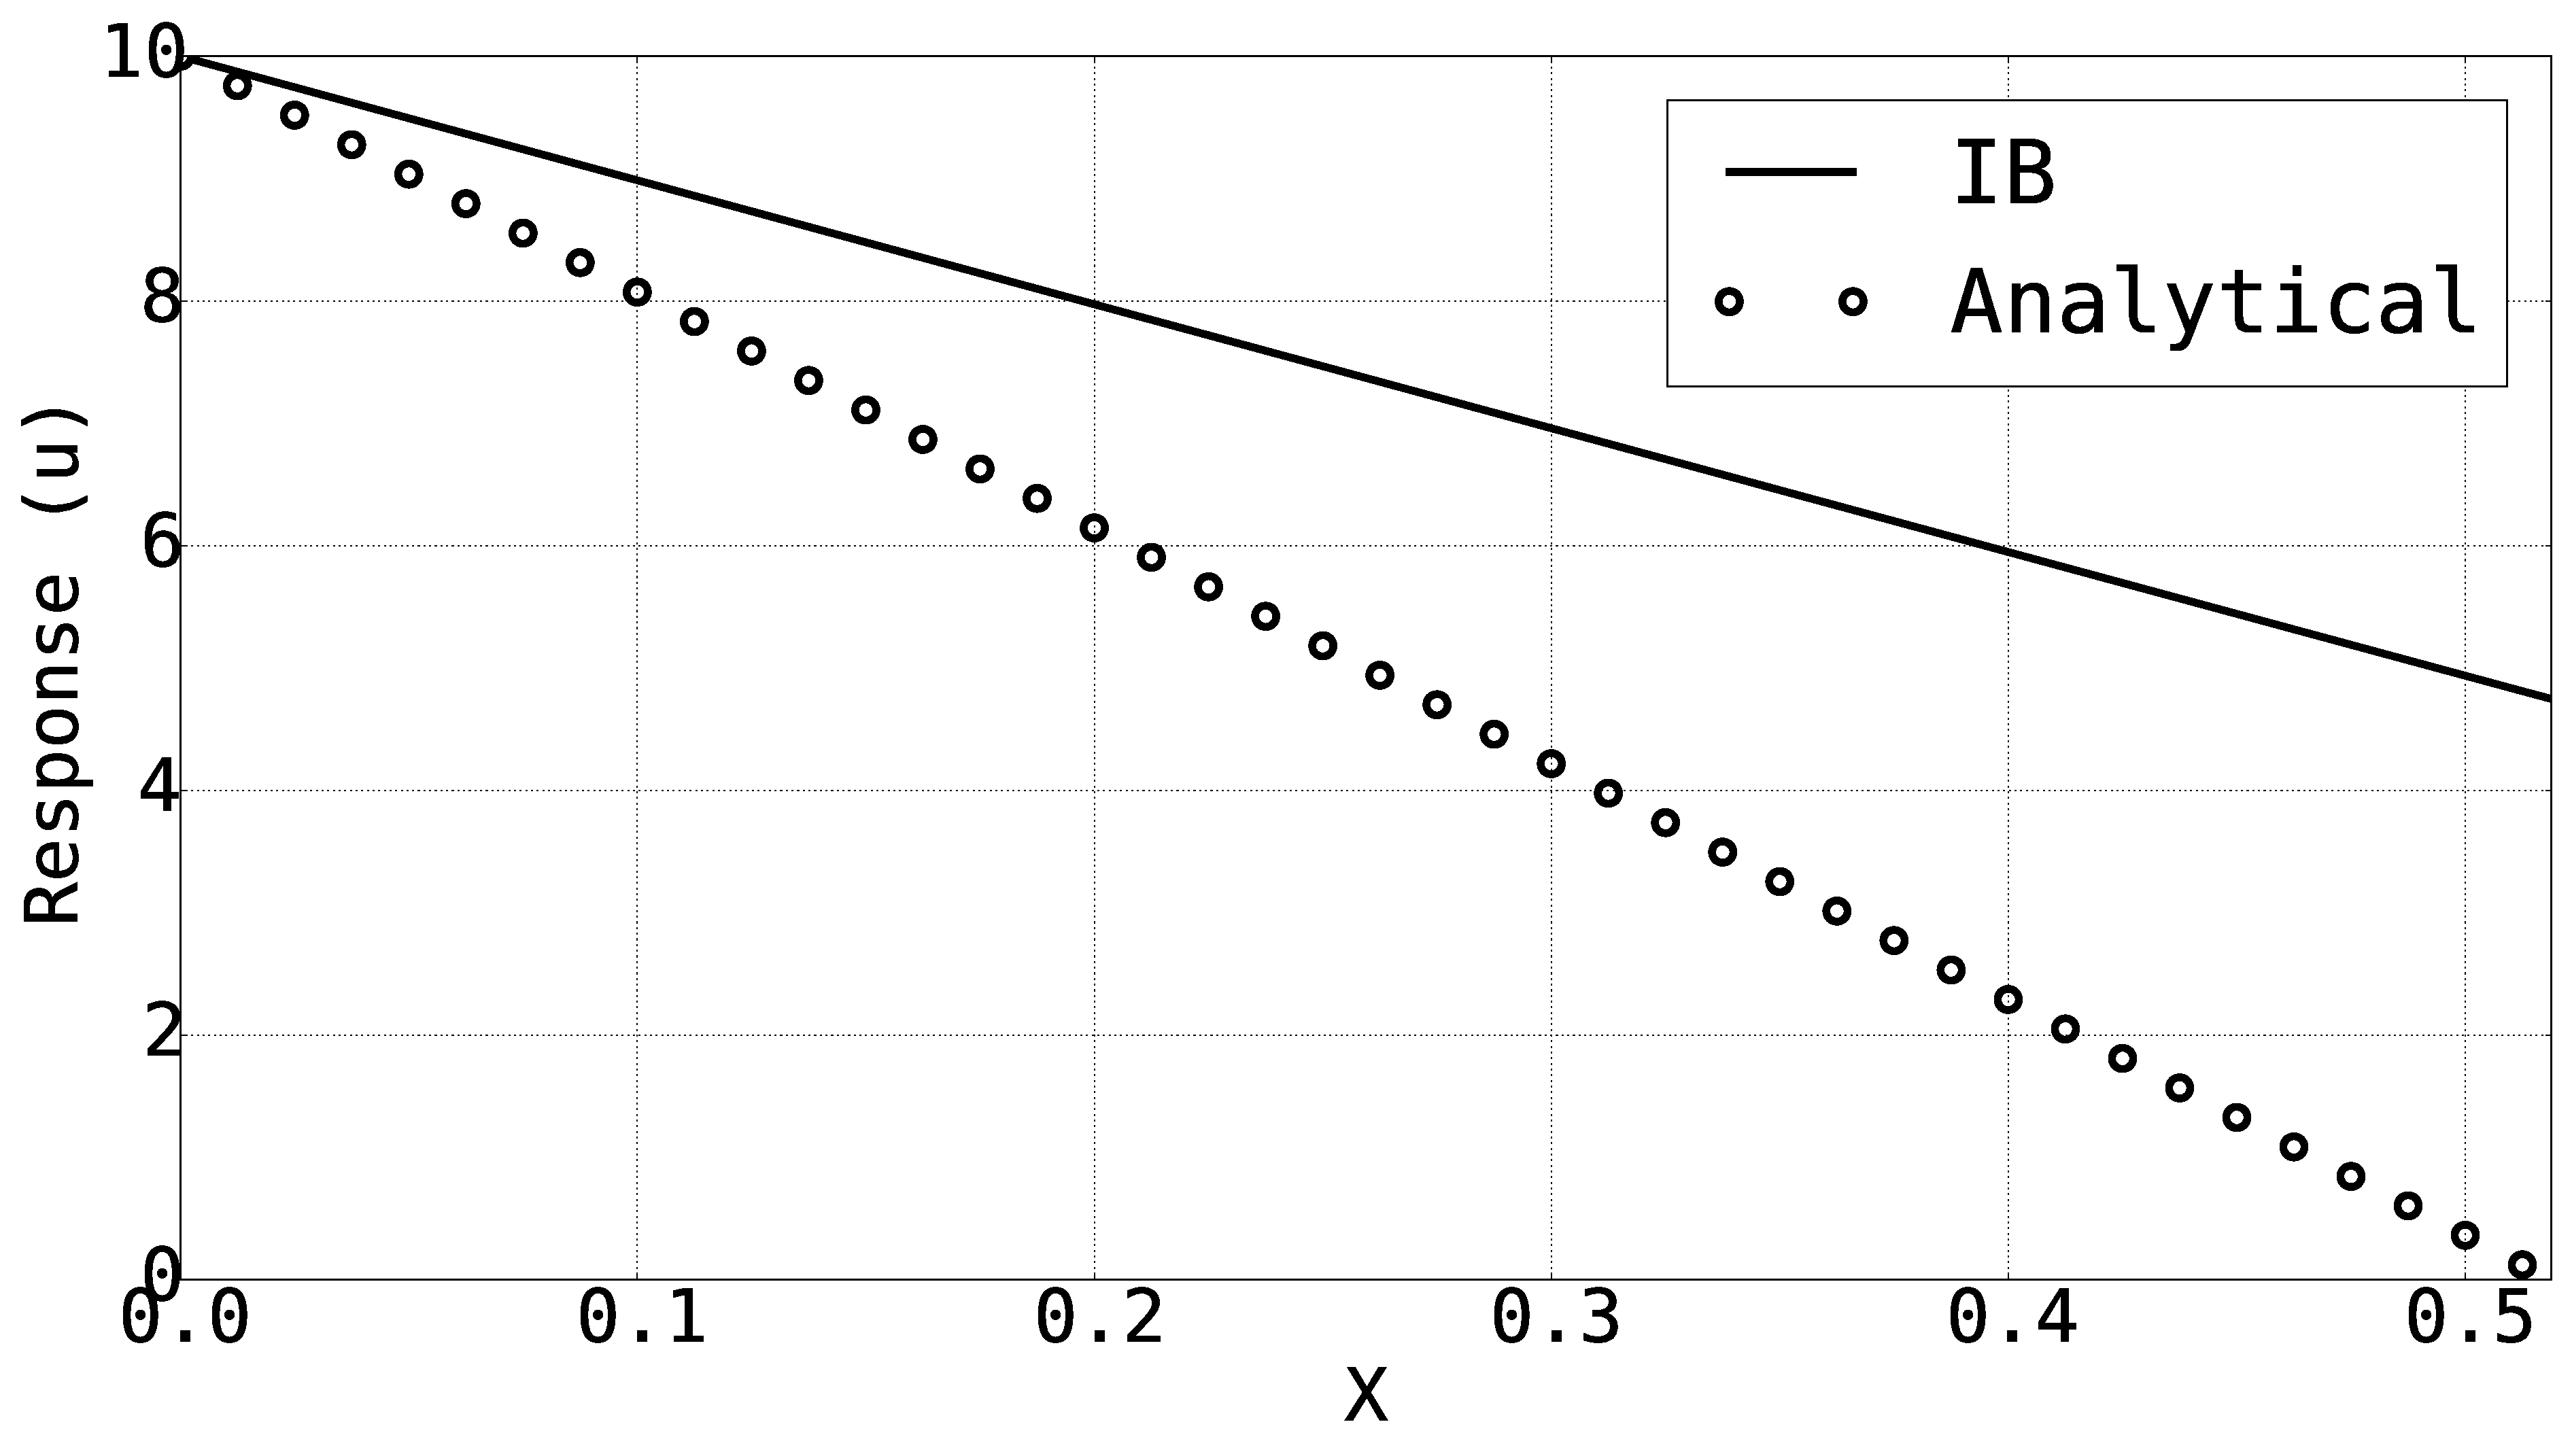
\includegraphics[width=7.0cm]{Chapter_3/figure/classicalIB_wallStiffness_2point_01.eps}
	}
	\quad
	\subfigure[$K_{wall} = 1$]
	{
	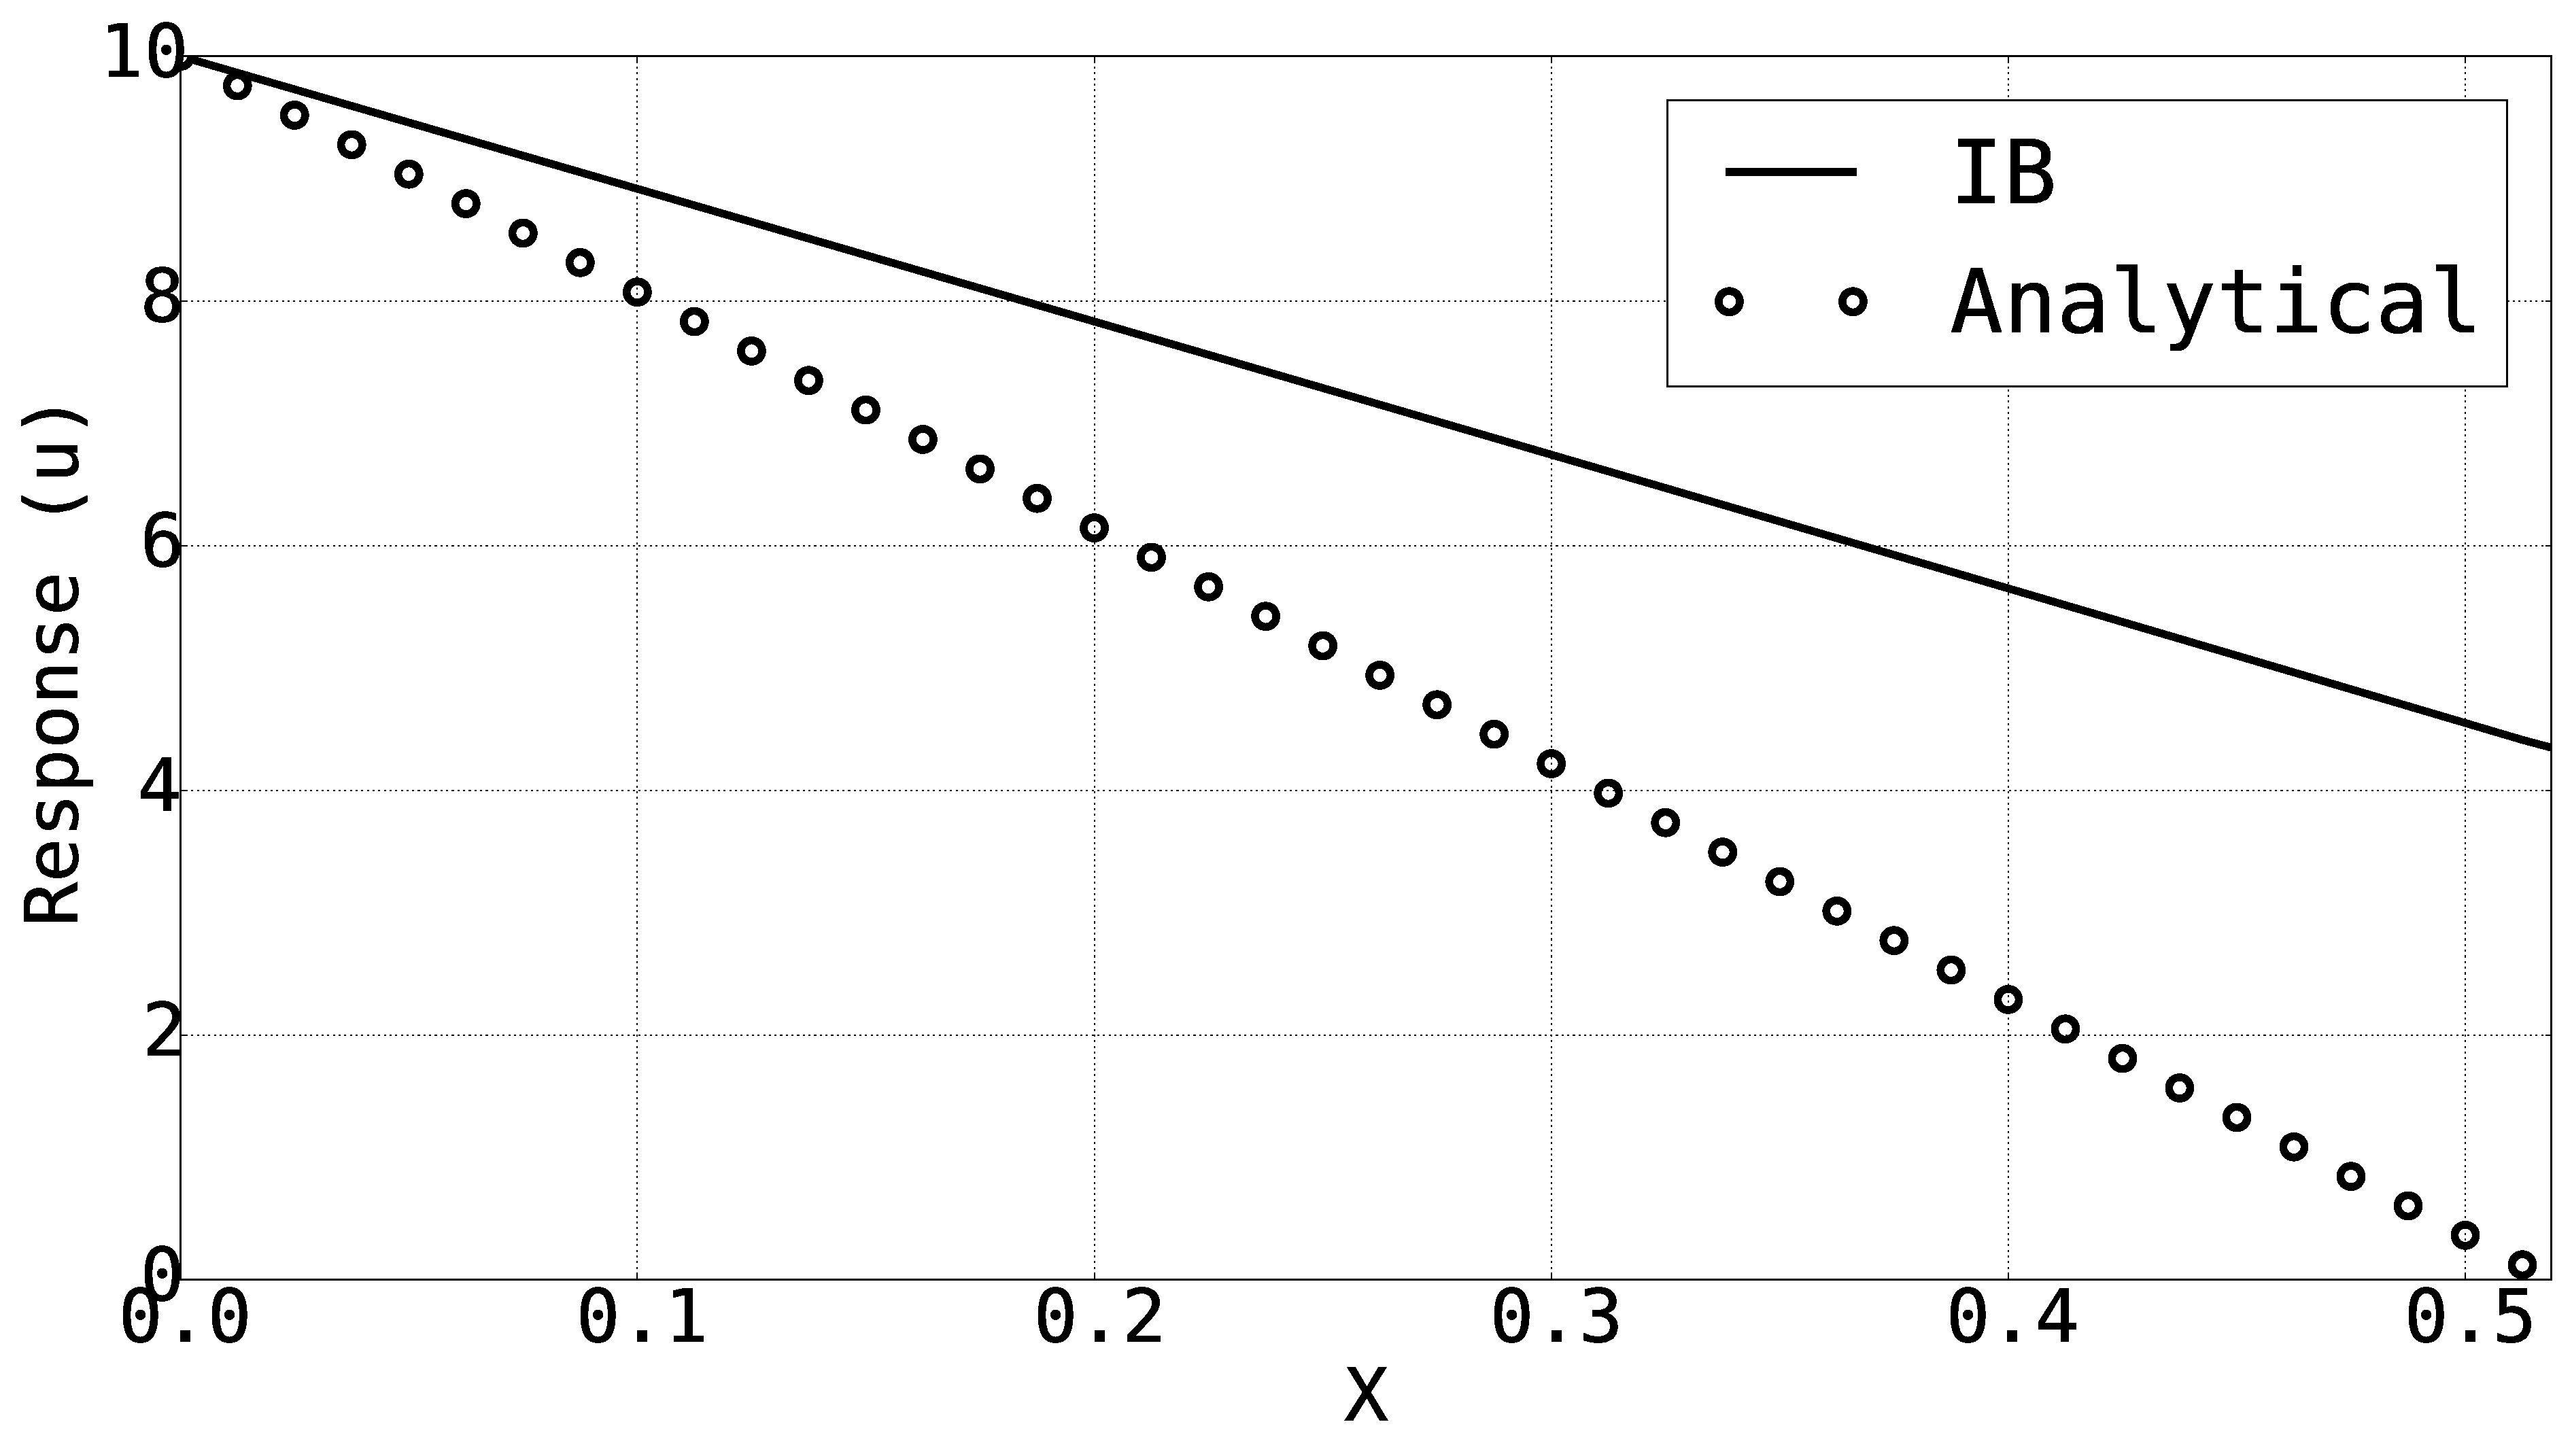
\includegraphics[width=7.0cm]{Chapter_3/figure/classicalIB_wallStiffness_2point_1.eps}
	}
	\\
	\subfigure[$K_{wall} = 10$]
	{
	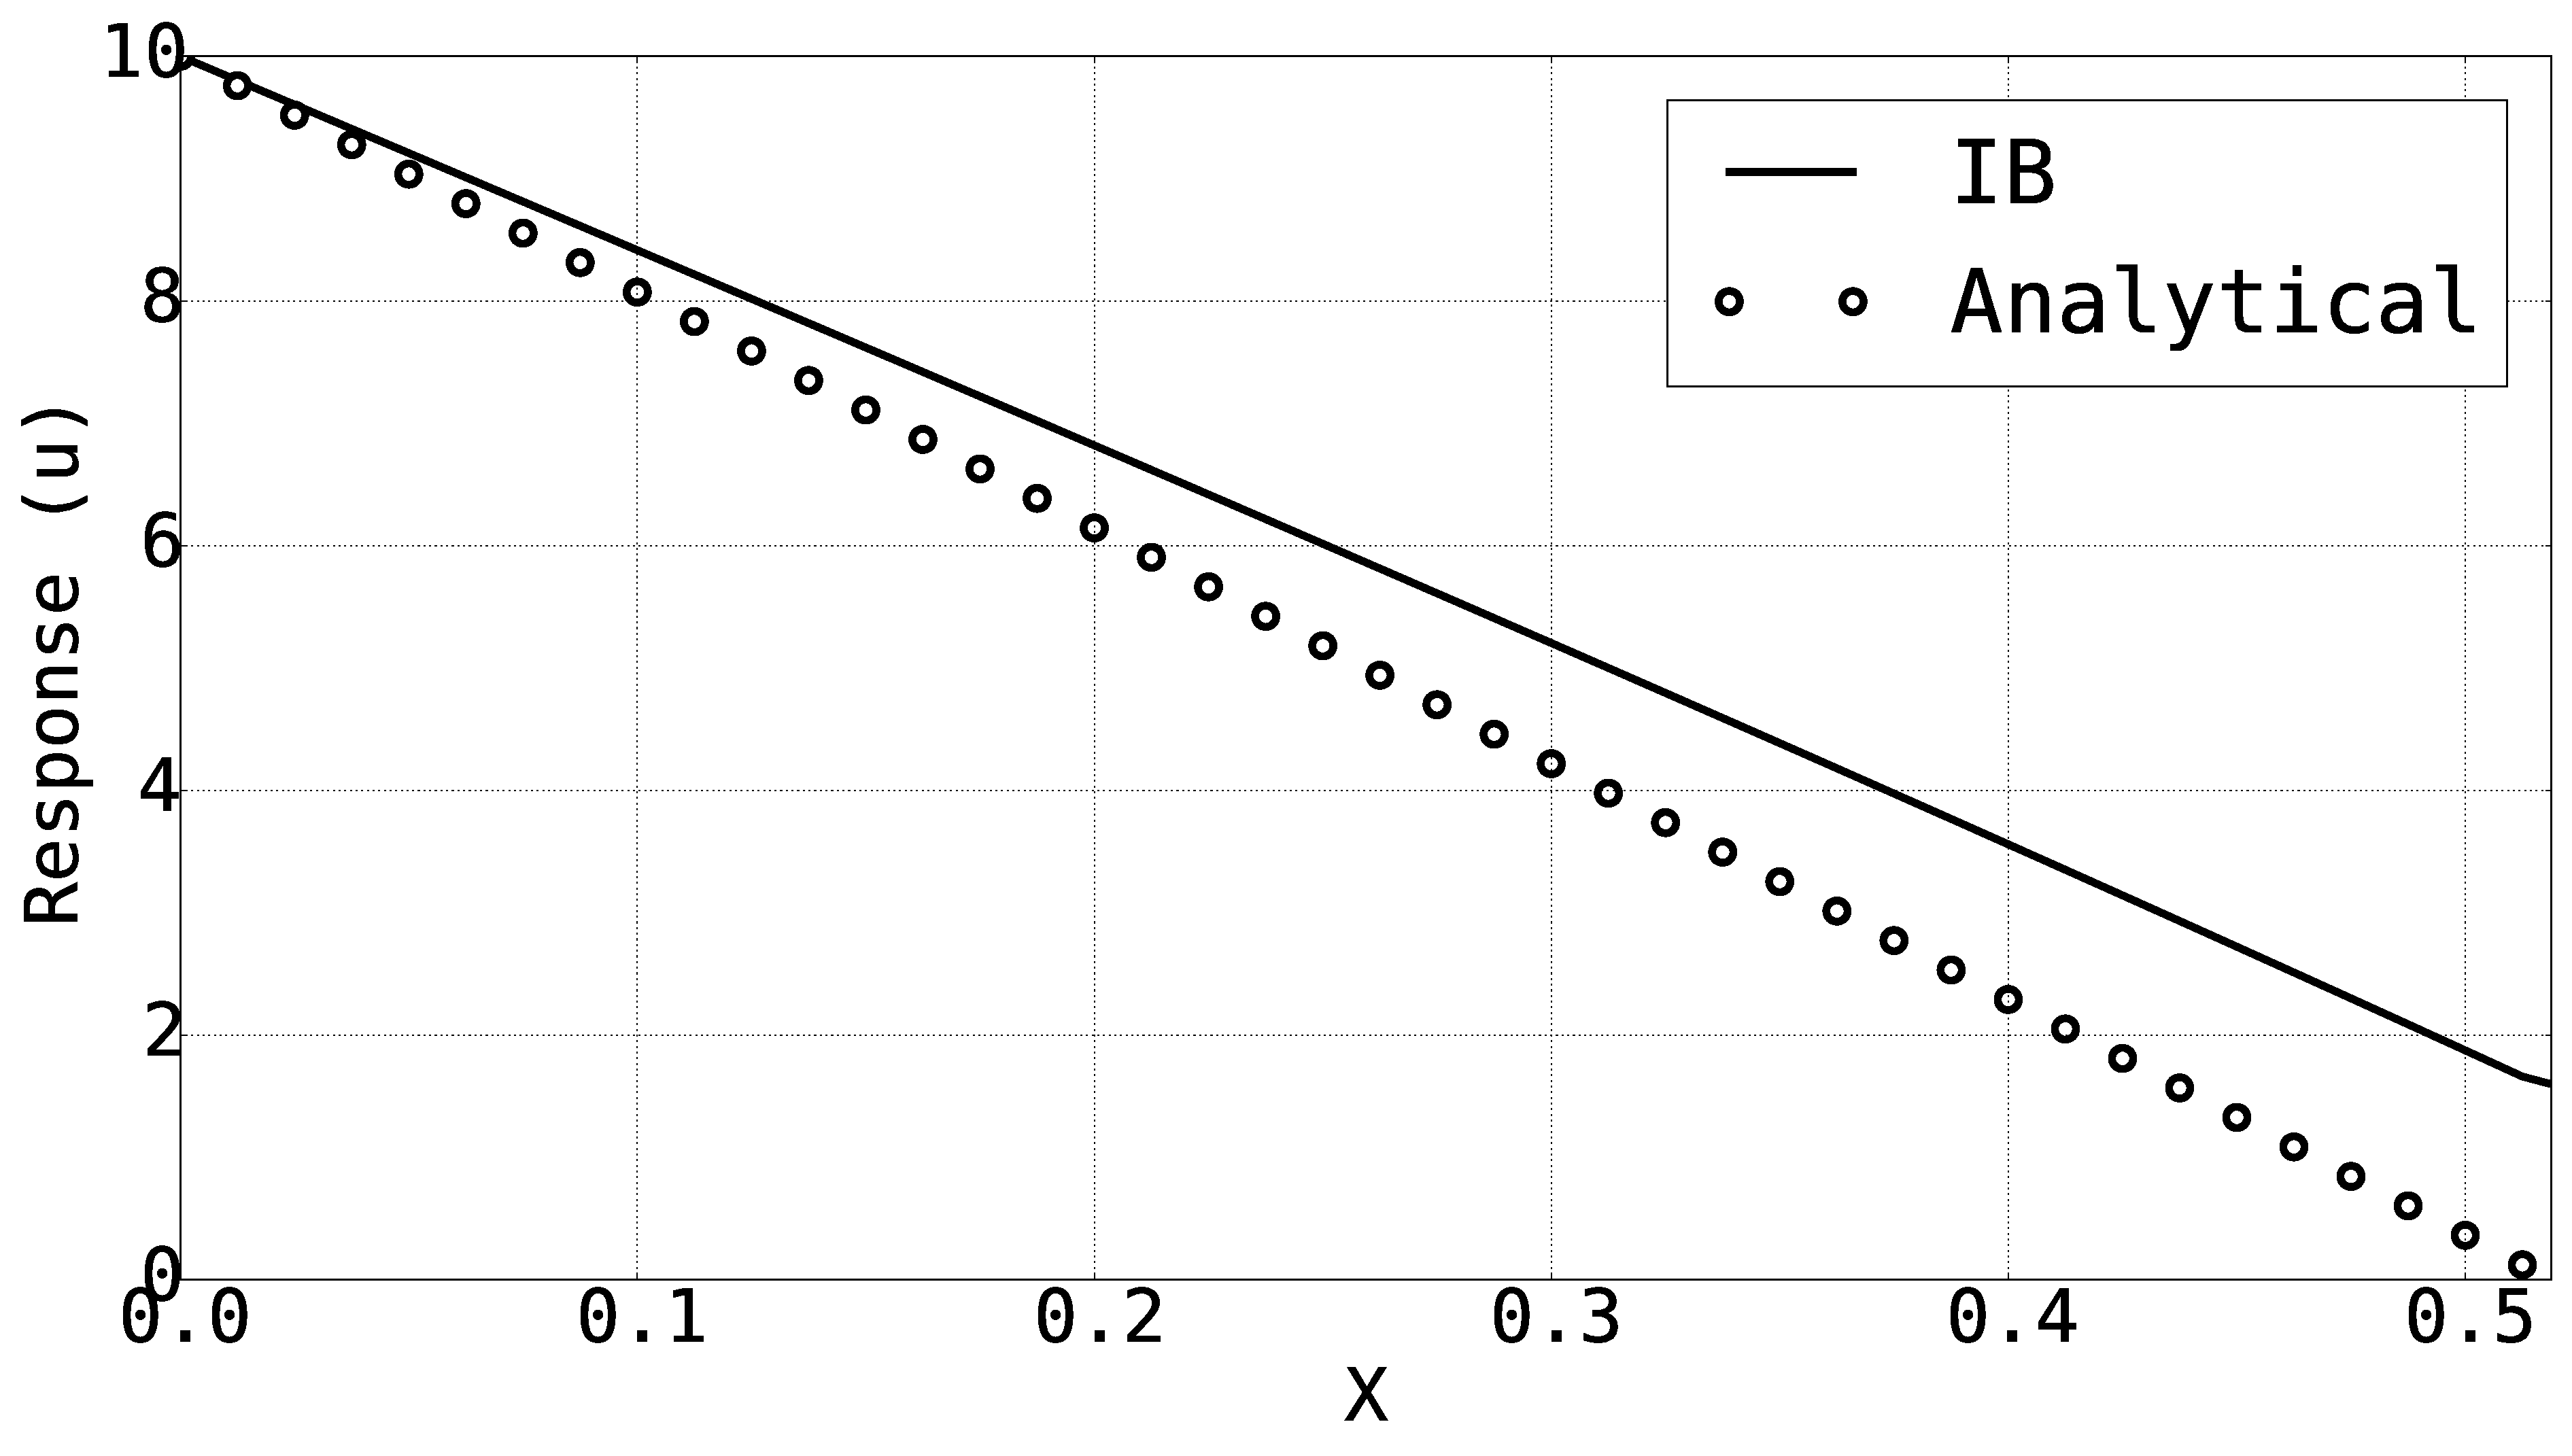
\includegraphics[width=7.0cm]{Chapter_3/figure/classicalIB_wallStiffness_2point_10.eps}
	}
	\quad
	\subfigure[$K_{wall} = 100$]
	{
	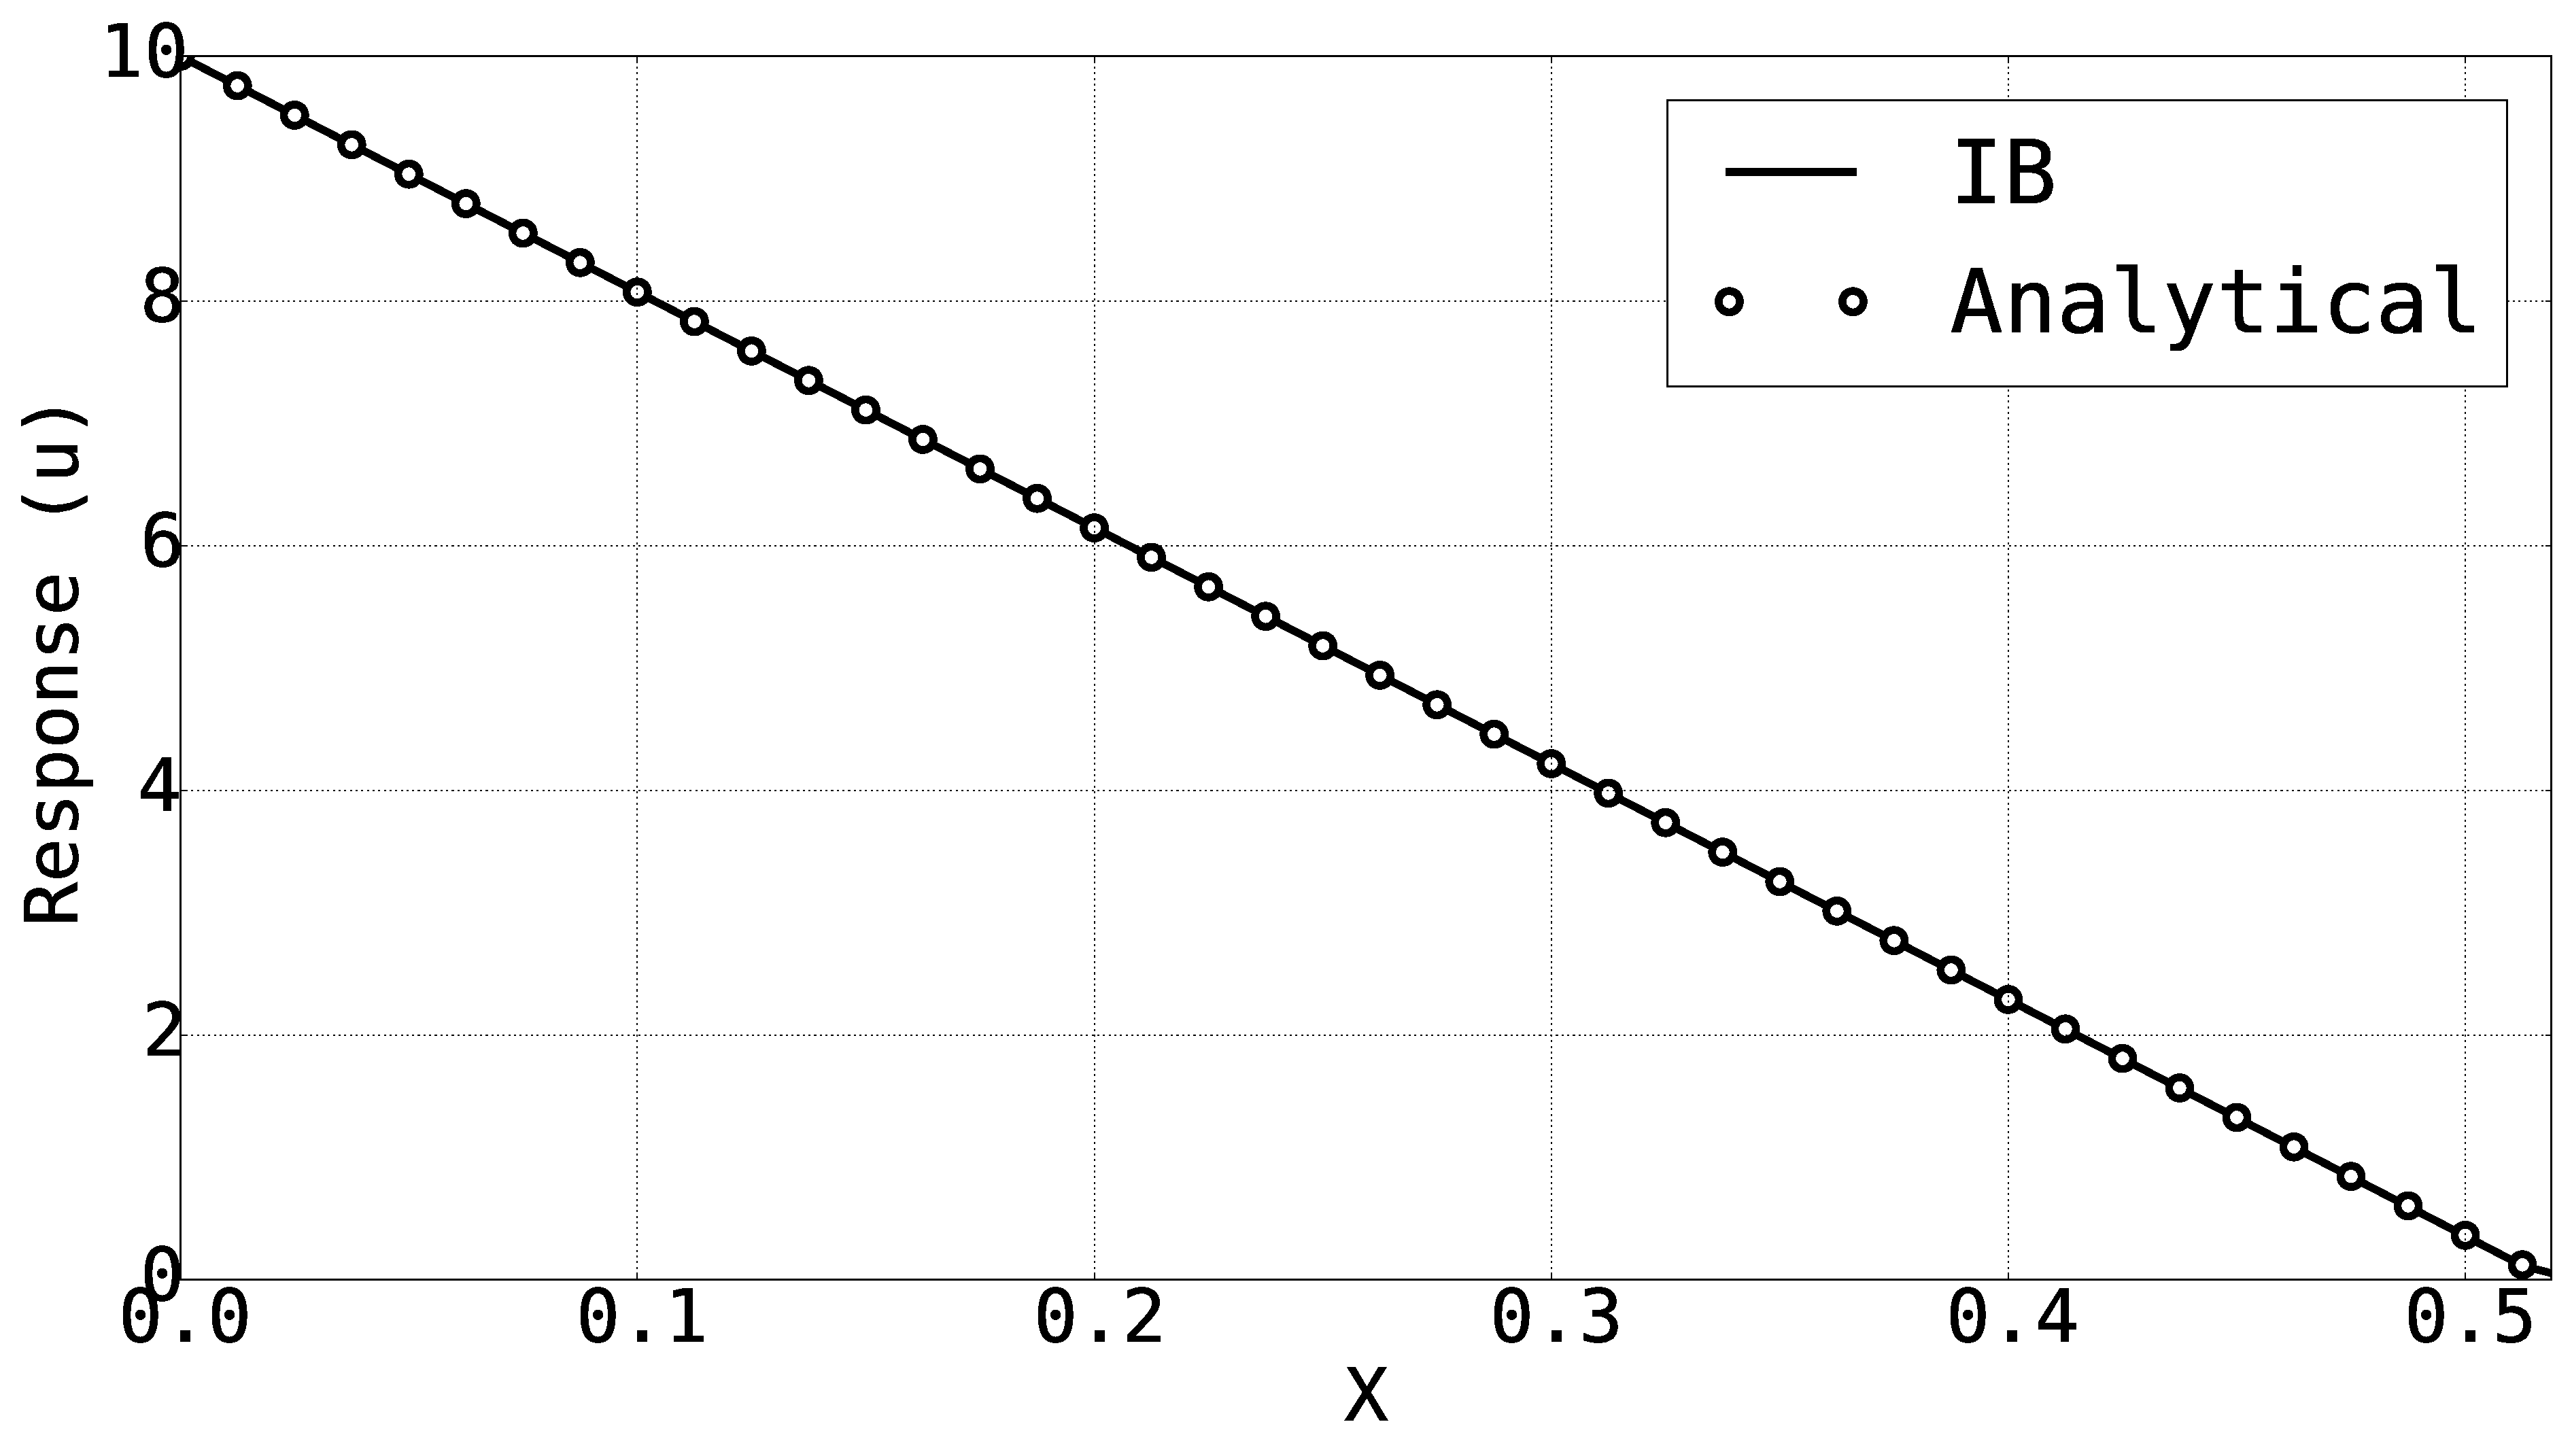
\includegraphics[width=7.0cm]{Chapter_3/figure/classicalIB_wallStiffness_2point_100.eps}
	}
	\caption{Comparison between IB and analytical results for different wall velocities.}
	\label{fig:C3_classicalIBResultWallStiffness}
\end{figure}

\begin{table}[H]
\centering
\begin{tabular}{c | c}
	 Wall velocity & RMSE \\ \hline \hline
	 0.1 & 0.1912 \\ \hline
	 1 & 0.1759  \\ \hline
	 10 & 0.0665 \\ \hline
	 100 & 0.001 \\
\end{tabular}
\caption{RMSE value for different wall stiffness values.}
\label{table:C3_classicalIBResultWallStiffnessRMSE}
\end{table}

% -.-.-.-.-.-.-.-.-.-.-.-.-.-.-.-.-.-.-.-.-.-.-.-.-.-.-.-.-.-.-.-.-.-
\subsection{Virtual boundary method}
The virtual boundary method is a different approach for imposing the effect of immersed boundary through force terms. This approach is well suited for both the rigid and elastic boundaries. The difference between this approach and the classical IB method is that it does not require the solution of the constitutive equations to calculate the force terms. This approach is based on the works of the works of Goldstein et al. \cite{goldstein1993modeling} to simulate the flow around the rigid bodies. The forcing term in the virtual boundary method is defined as

\begin{equation}\label{eq:C3_virtualBoundaryMethod}
	F(X_k, t) = 
	\alpha \int_0^t \left[ u(X_k, t) - U(X_k, t) \right] dt + 
	\beta \left[ u(X_k, t) - U(X_k, t) \right]
\end{equation}

where $F$ is the required force at the $k$-th Lagrangian point, $u(X_k, t)$ is the velocity calculated from the the Eulerian nodes using the $\delta$ function, and $U(X_k)$ is the desired velocity at the Lagrangian point $X_k$. The coefficient $\alpha$ and $\beta$ are selected to best enforce the boundary condition at the immersed solid boundary. Equation \eqref{eq:C3_virtualBoundaryMethod} is essentially a way to provide a feedback control to the system to make sure that the desired velocity ($U(X_k, t)$) is achieved at the immersed boundary. From a physical stand point, this equation represents a damped oscillator \cite{iaccarino2003immersed}.

As before, we apply this technique to the demonstration problem defined in Section \ref{sec:C3_benchmark_case}. We use the Crank-Nicholson method to discretize the equations as shown in the following equation. 

\begin{equation}\label{eq:C3_virtualBoundaryDiscretization}
	\frac{u^{n+1} - u^n}{\Delta t} = 
	\frac{1}{2}
	\left(
	\frac{\partial^2 u^{n+1}}{\partial x^2} +
	\frac{\partial^2 u^{n}}{\partial x^2}
	\right)
\end{equation}

where $n$ is the time step that we are at. The steps to solve this problem using the virtual boundary method can be defined as follows

\begin{enumerate}
	\item Define the initial condition as $u^0$ and set $f^0$ equal to zero.
	\item Calculate the velocity at the next time step, $u^1$, using Equation \eqref{eq:C3_discretizedEquationPeskinIB}
	\item Map the velocity results to the Lagrangian nodes using the $\delta$ function
	\item Based on the new velocity at $t=1$ evaluate Equation \eqref{eq:C3_virtualBoundaryMethod}.
	\item Map the force at the Lagrangian location $X$ to its neighbouring Eulerian points using $\delta$ function.
	\item Reiterate until the convergence is satisfied.
\end{enumerate}

Comparing the virtual boundary method to the classical IB method, we can see that less steps are required for this formulation. Moreover, there is no need to solve the constitutive equation for the solid domain which reduces the total computational cost.

Like the classical IB method, we investigate the effect of mesh size, moving wall velocity, and values for $\alpha$ and $\beta$ constants of the solution accuracy. The numerical results are verified with the analytical solution of this problem. We use the RMSE value as a metric to compare the results.

We looked at the effect of mesh size on the solution accuracy of the virtual boundary method. For this case, the moving wall velocity is fixed at $10 m/s$ with the location of fixed wall at $x_{wall} = 0.726$. The time step for this simulation is chosen as $10^{-5}$ with $\alpha = -1000$ and $\beta = -10$. We chose the node number as $11$, $41$, $81$, and $161$. The total length of the domain is chosen as $1 m$. As shown in Figure \ref{C3_virtualBoundaryResultNodeNumber} and Table \ref{table:C3_virtualBoundaryResultNodeNumberRMSE}, by increasing the nodes number the simulation results become more accurate. However, the convergence is reached earlier compared to the classical IB method of last section. This means that the computational effort to get the same accuracy compared to classical IB method is much less when using the virtual boundary method. 

\begin{figure}[H]
	\centering
	\subfigure[N = 11]
	{
	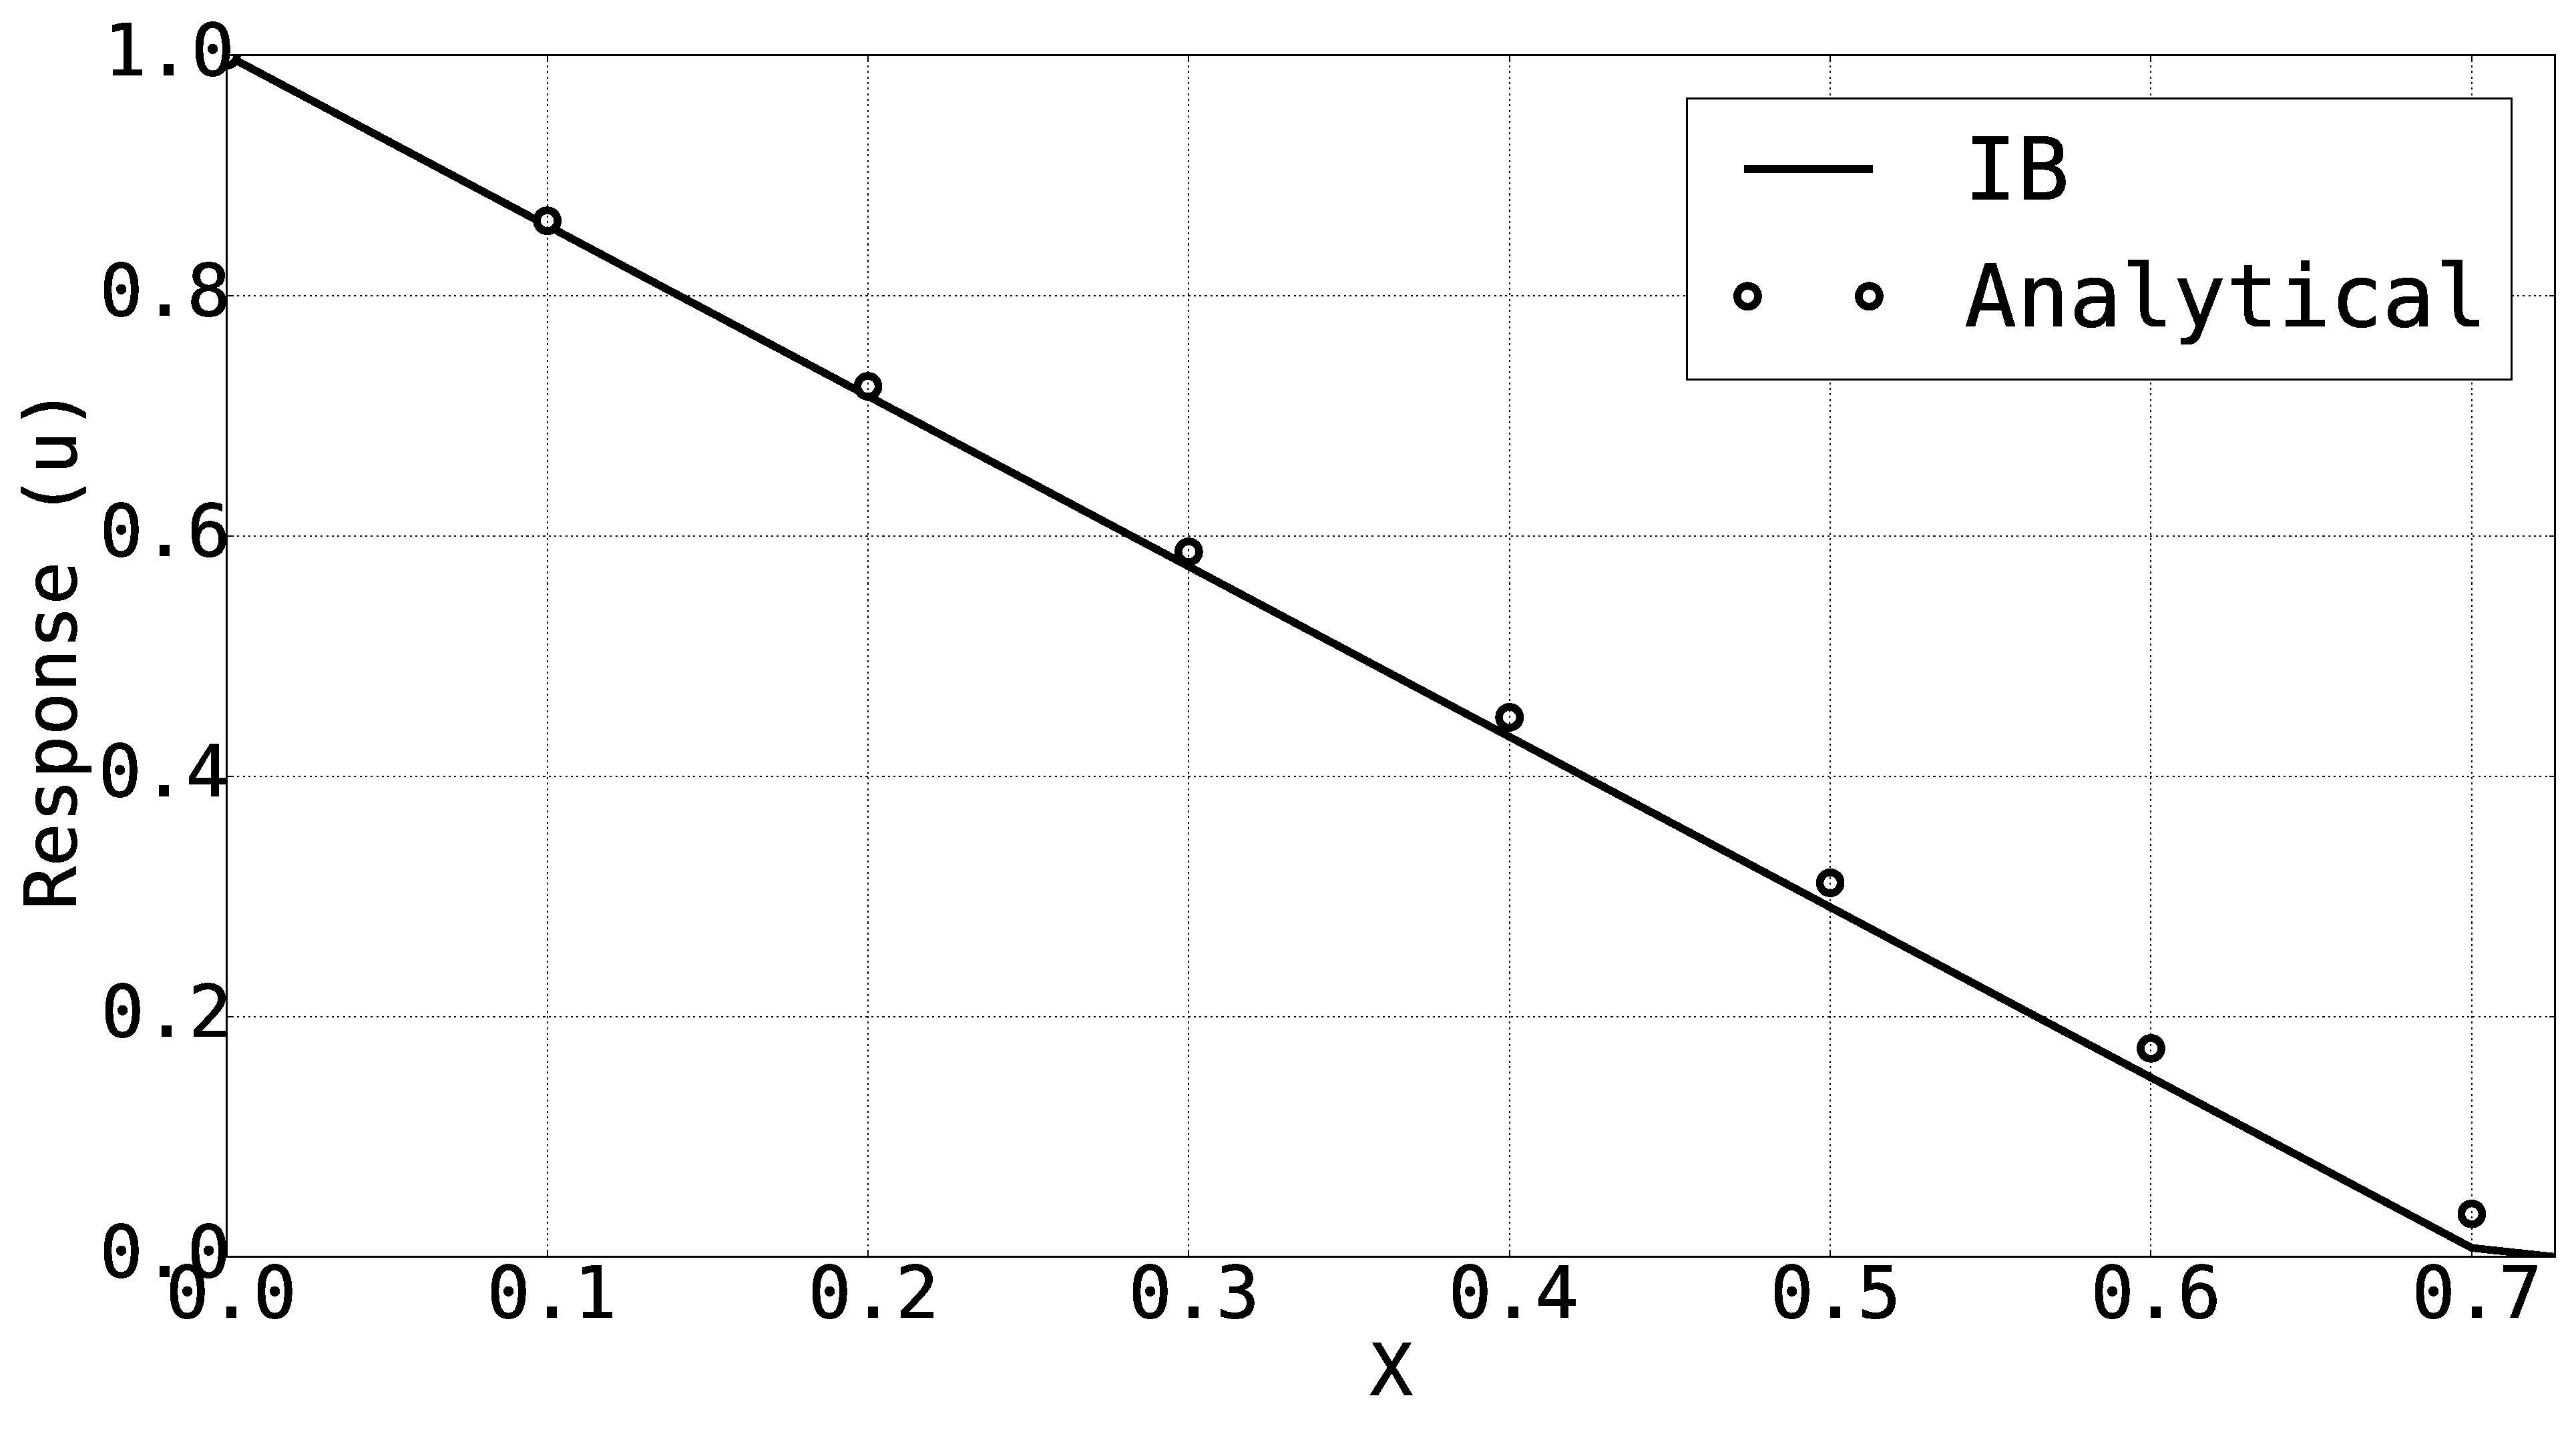
\includegraphics[width=7.0cm]{Chapter_3/figure/virtualBoundary_nodeNumber_11.eps}
	}
	\quad
	\subfigure[N = 41]
	{
	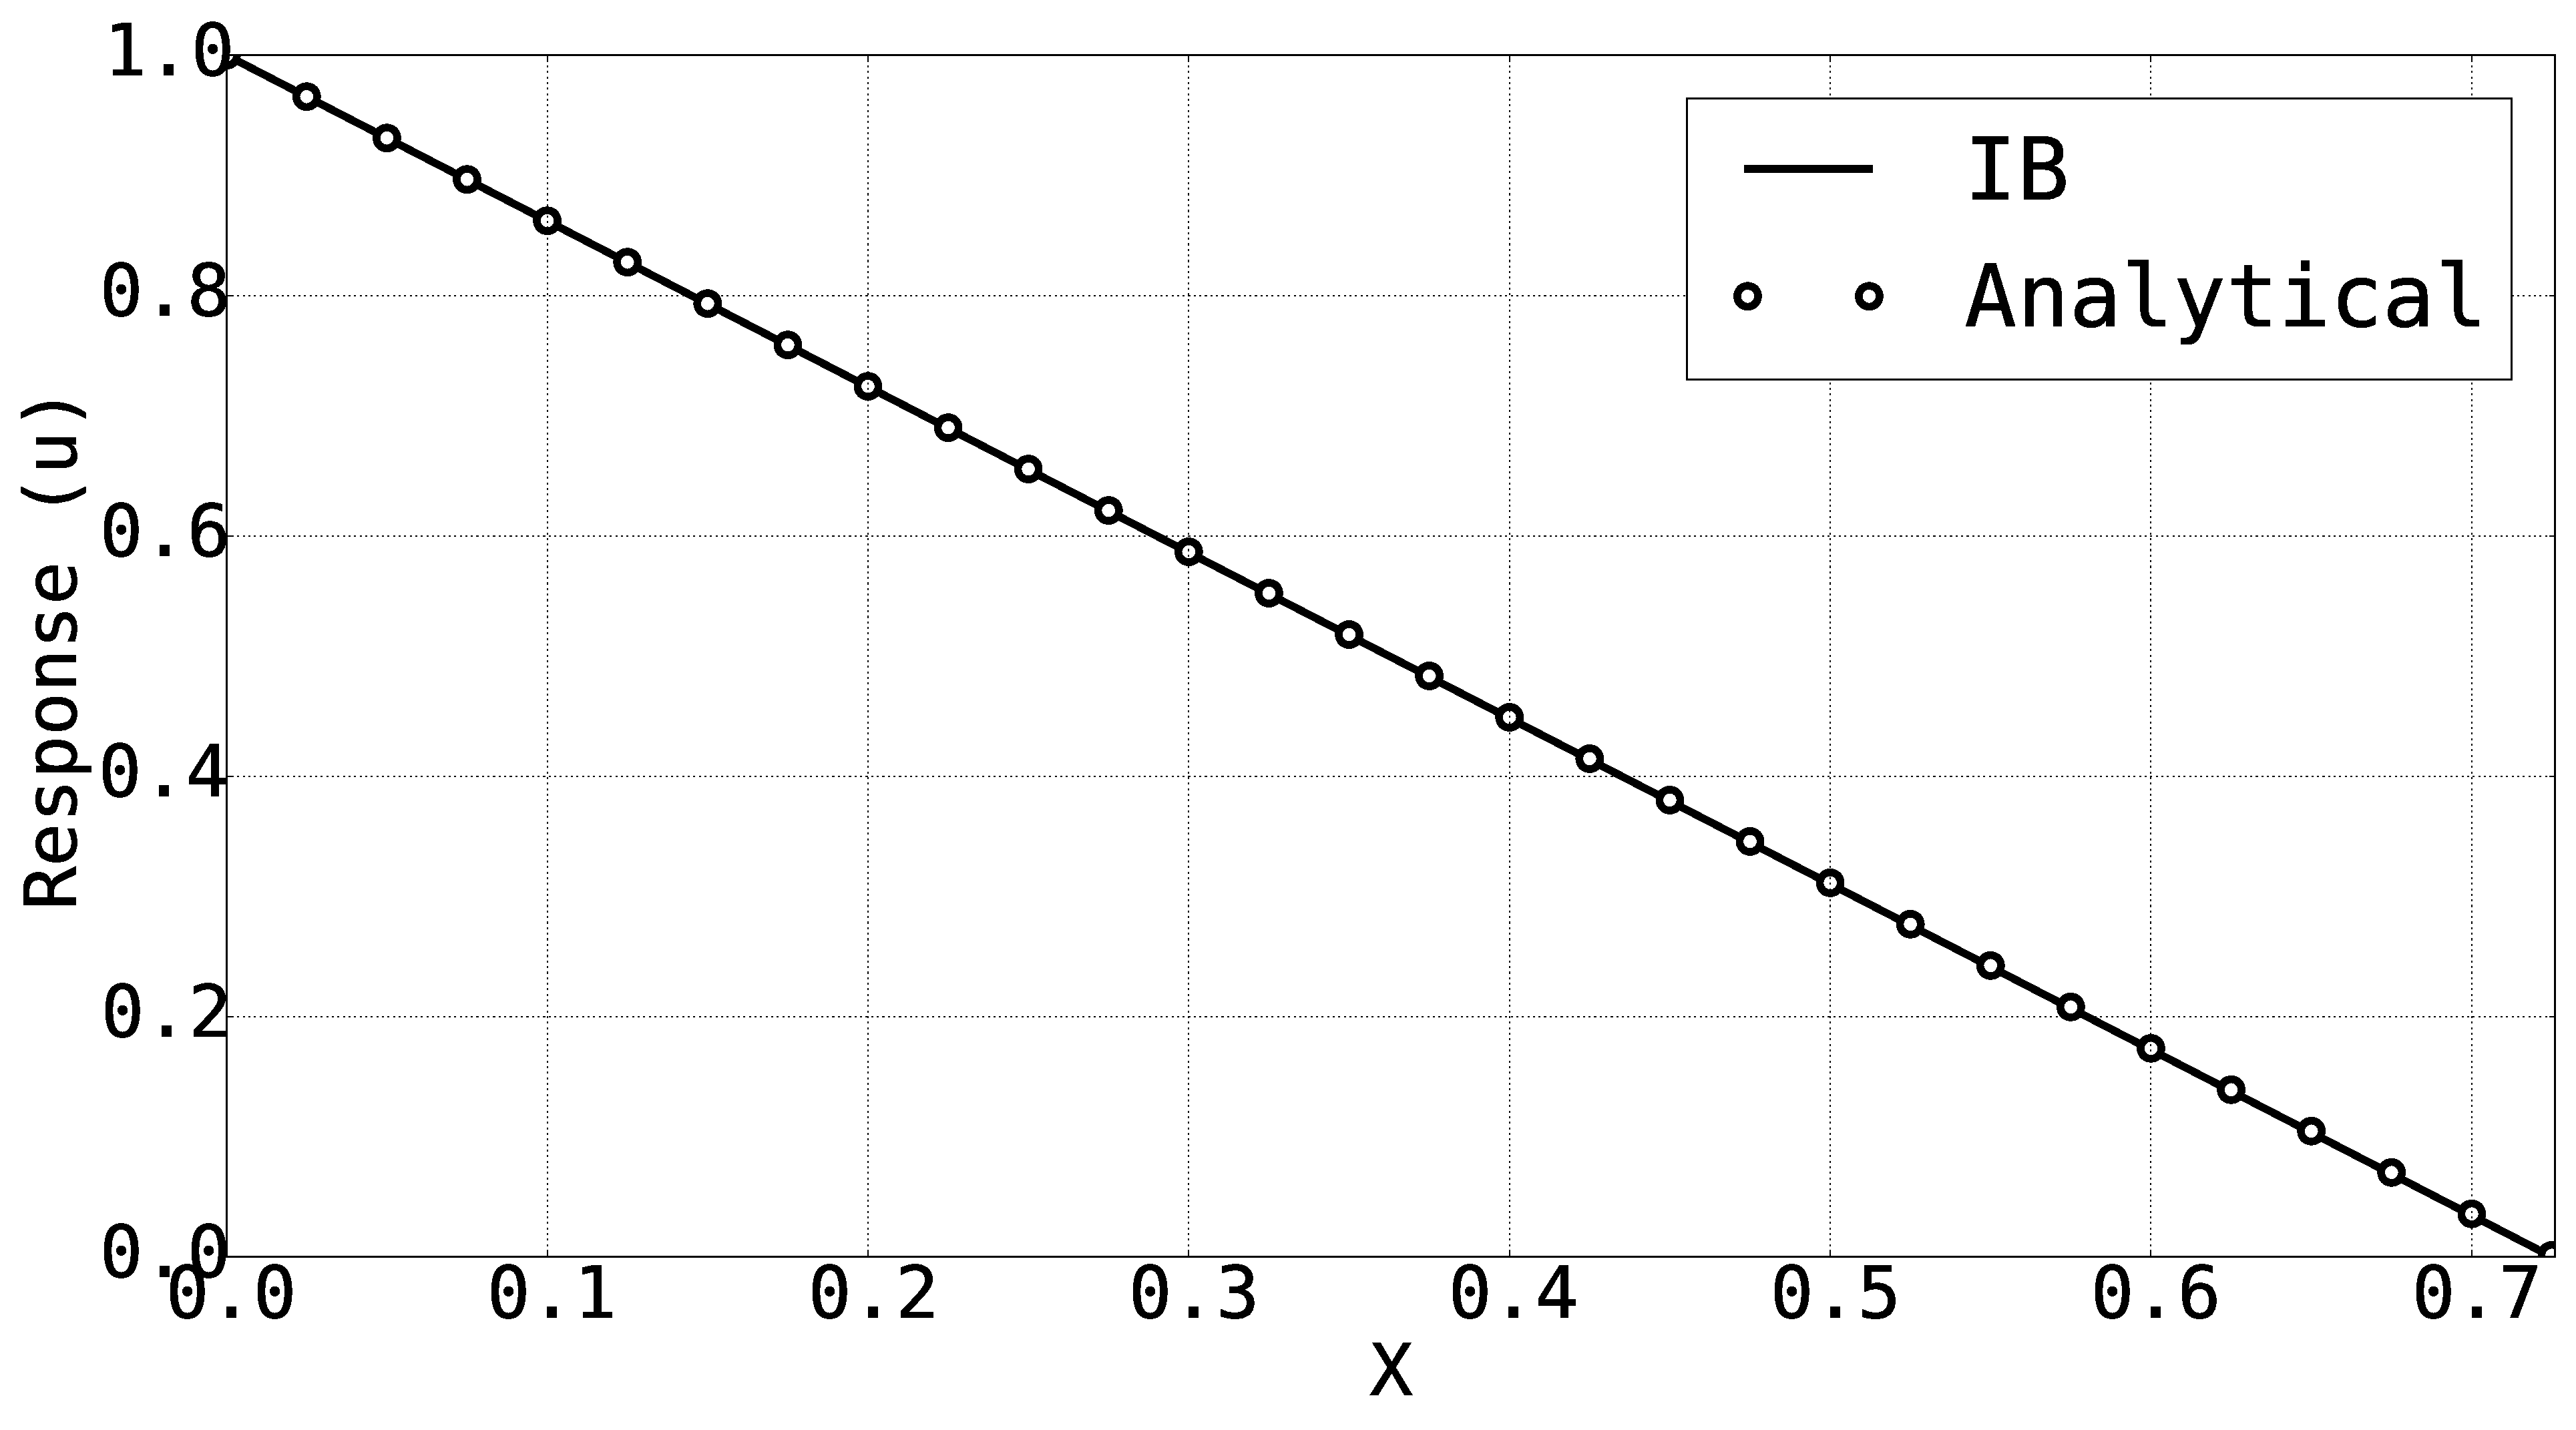
\includegraphics[width=7.0cm]{Chapter_3/figure/virtualBoundary_nodeNumber_41.eps}
	}
	\\
	\subfigure[N = 81]
	{
	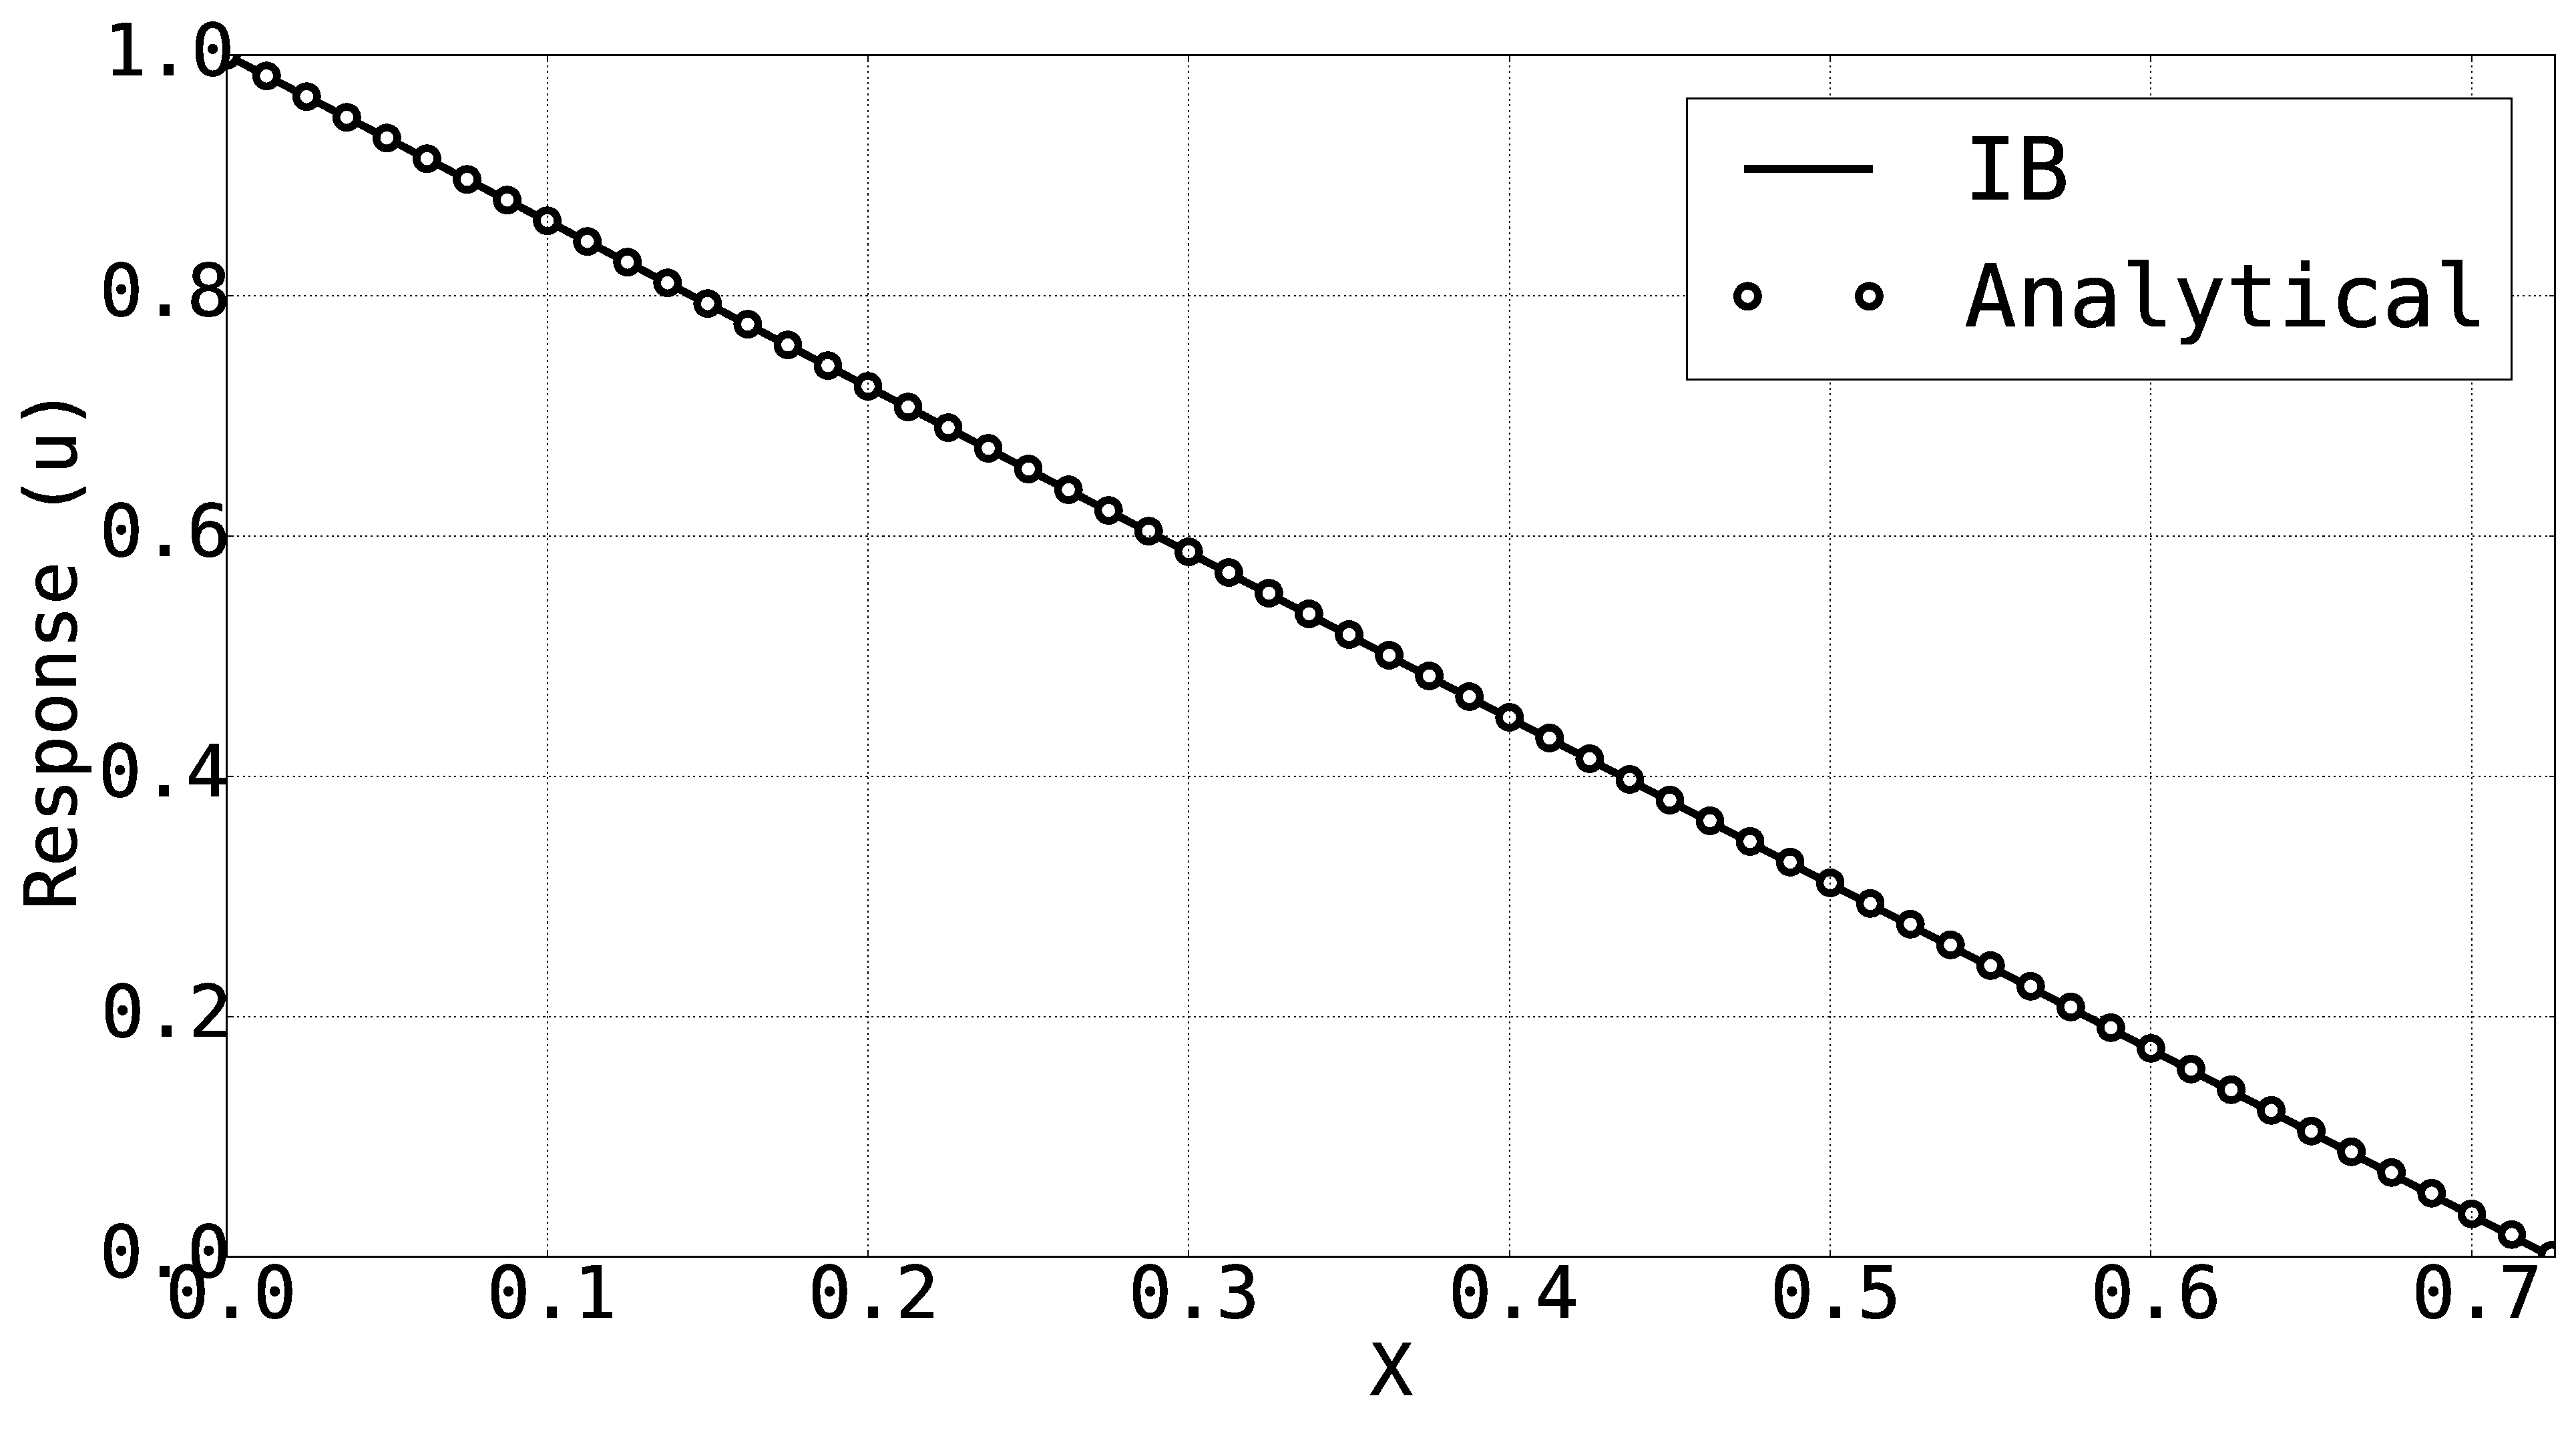
\includegraphics[width=7.0cm]{Chapter_3/figure/virtualBoundary_nodeNumber_81.eps}
	}
	\quad
	\subfigure[N = 161]
	{
	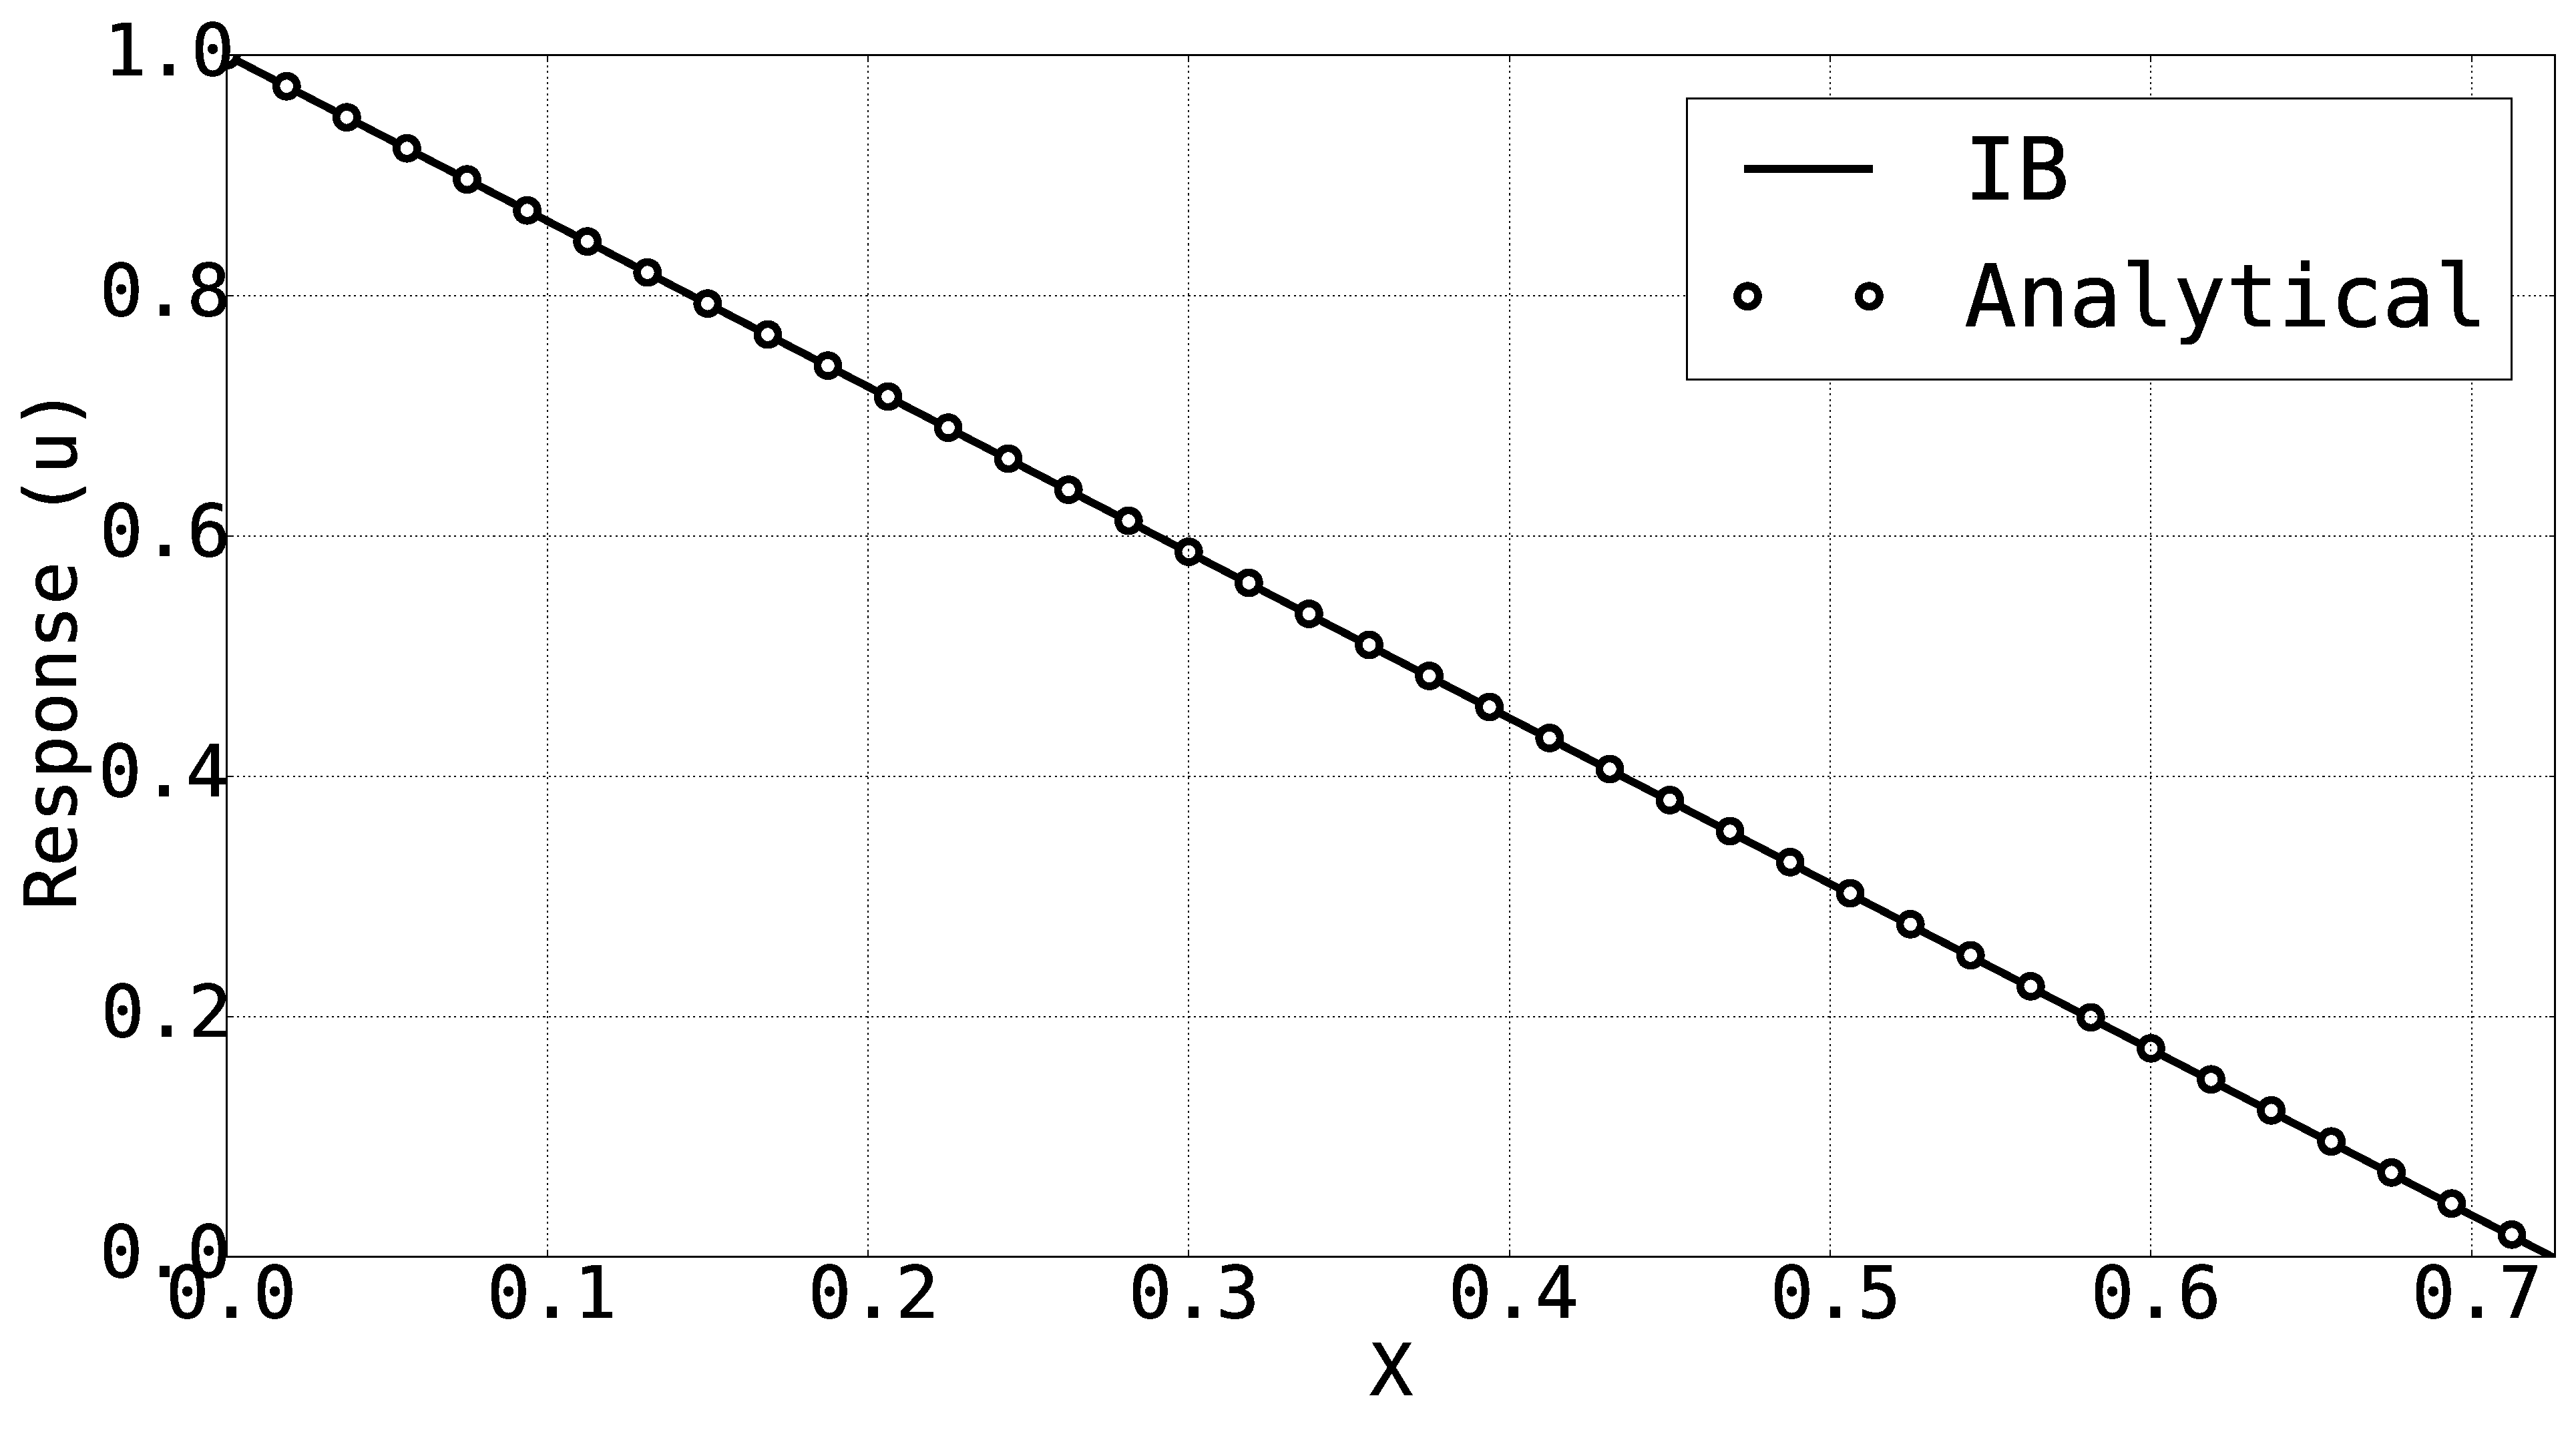
\includegraphics[width=7.0cm]{Chapter_3/figure/virtualBoundary_nodeNumber_161.eps}
	}
	\caption{Comparison between IB and analytical results for different porosity values.}
	\label{fig:C3_virtualBoundaryResultNodeNumber}
\end{figure}

\begin{table}[H]
\centering
\begin{tabular}{c | c }
	 Node number & RMSE \\ \hline \hline
	 11 & 0.012 \\ \hline
	 41 & 0.00065 \\ \hline
	 81 & 0.00063 \\ \hline
	 161 & 0.00058 \\
\end{tabular}
\caption{RMSE value for different node numbers.}
\label{table:C3_virtualBoundaryResultNodeNumberRMSE}
\end{table}

We looked at the effect of wall velocity of the solution accuracy. As before the length of the domain is fixed at $1 m$ with wall defined at $x_{wall} = 0.726$, the time step is chosen as $10^{-5}$. We chose the $\alpha$ and $\beta$ constants as $-1000$ and $-10$ respectively. We simulated the flow selecting the wall velocity as $10$, $100$, $1000$, and $10000$. The results are compared with the analytical results. As shown in Figure \ref{fig:C3_virtualBoundaryResultWallVelocity} and Table \ref{table:C3_virtualBoundaryResultWallVelocityRMSE}, the wall velocity does not affect the accuracy of the solution. When compared with the results of the classical IB method in previous section, we can see that the virtual boundary method produces more accurate results. Moreover, the simulation time is much less than the classical IB method.

\begin{figure}[H]
	\centering
	\subfigure[$u_{wall} = 10 m/s$]
	{
	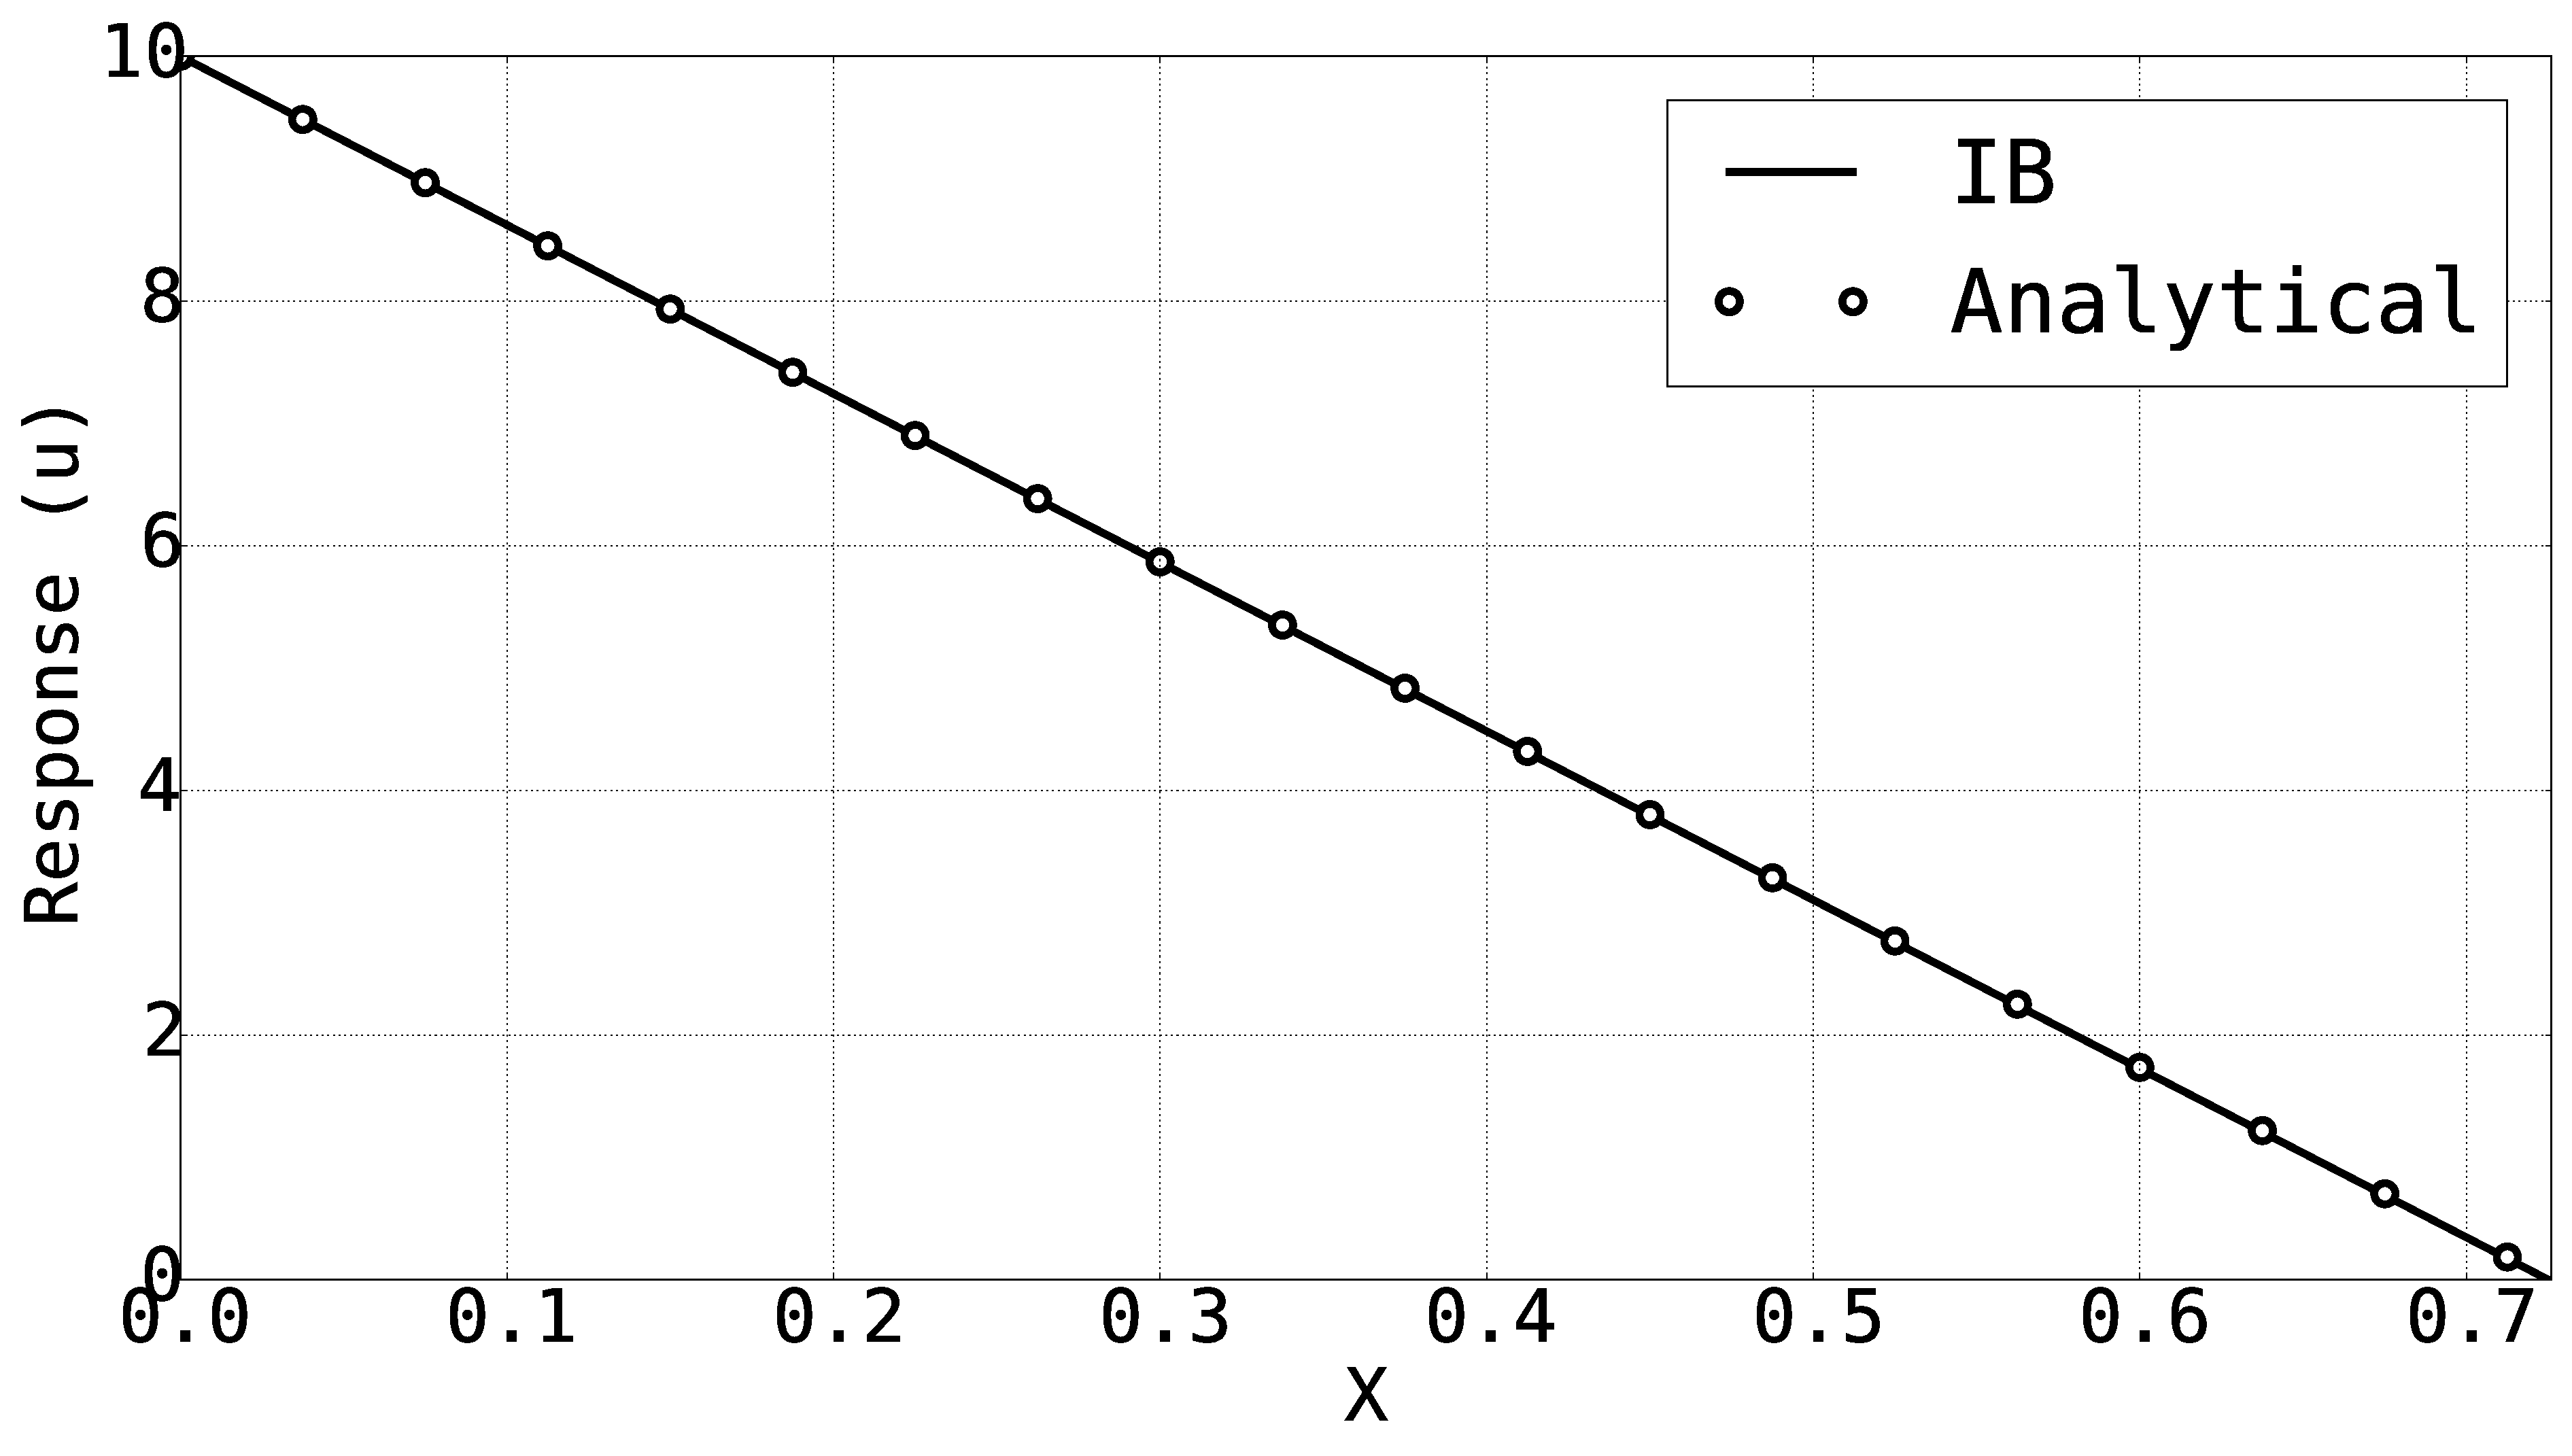
\includegraphics[width=7.0cm]{Chapter_3/figure/virtualBoundary_wallVelocity_10.eps}
	}
	\quad
	\subfigure[$u_{wall} = 10^2 m/s$]
	{
	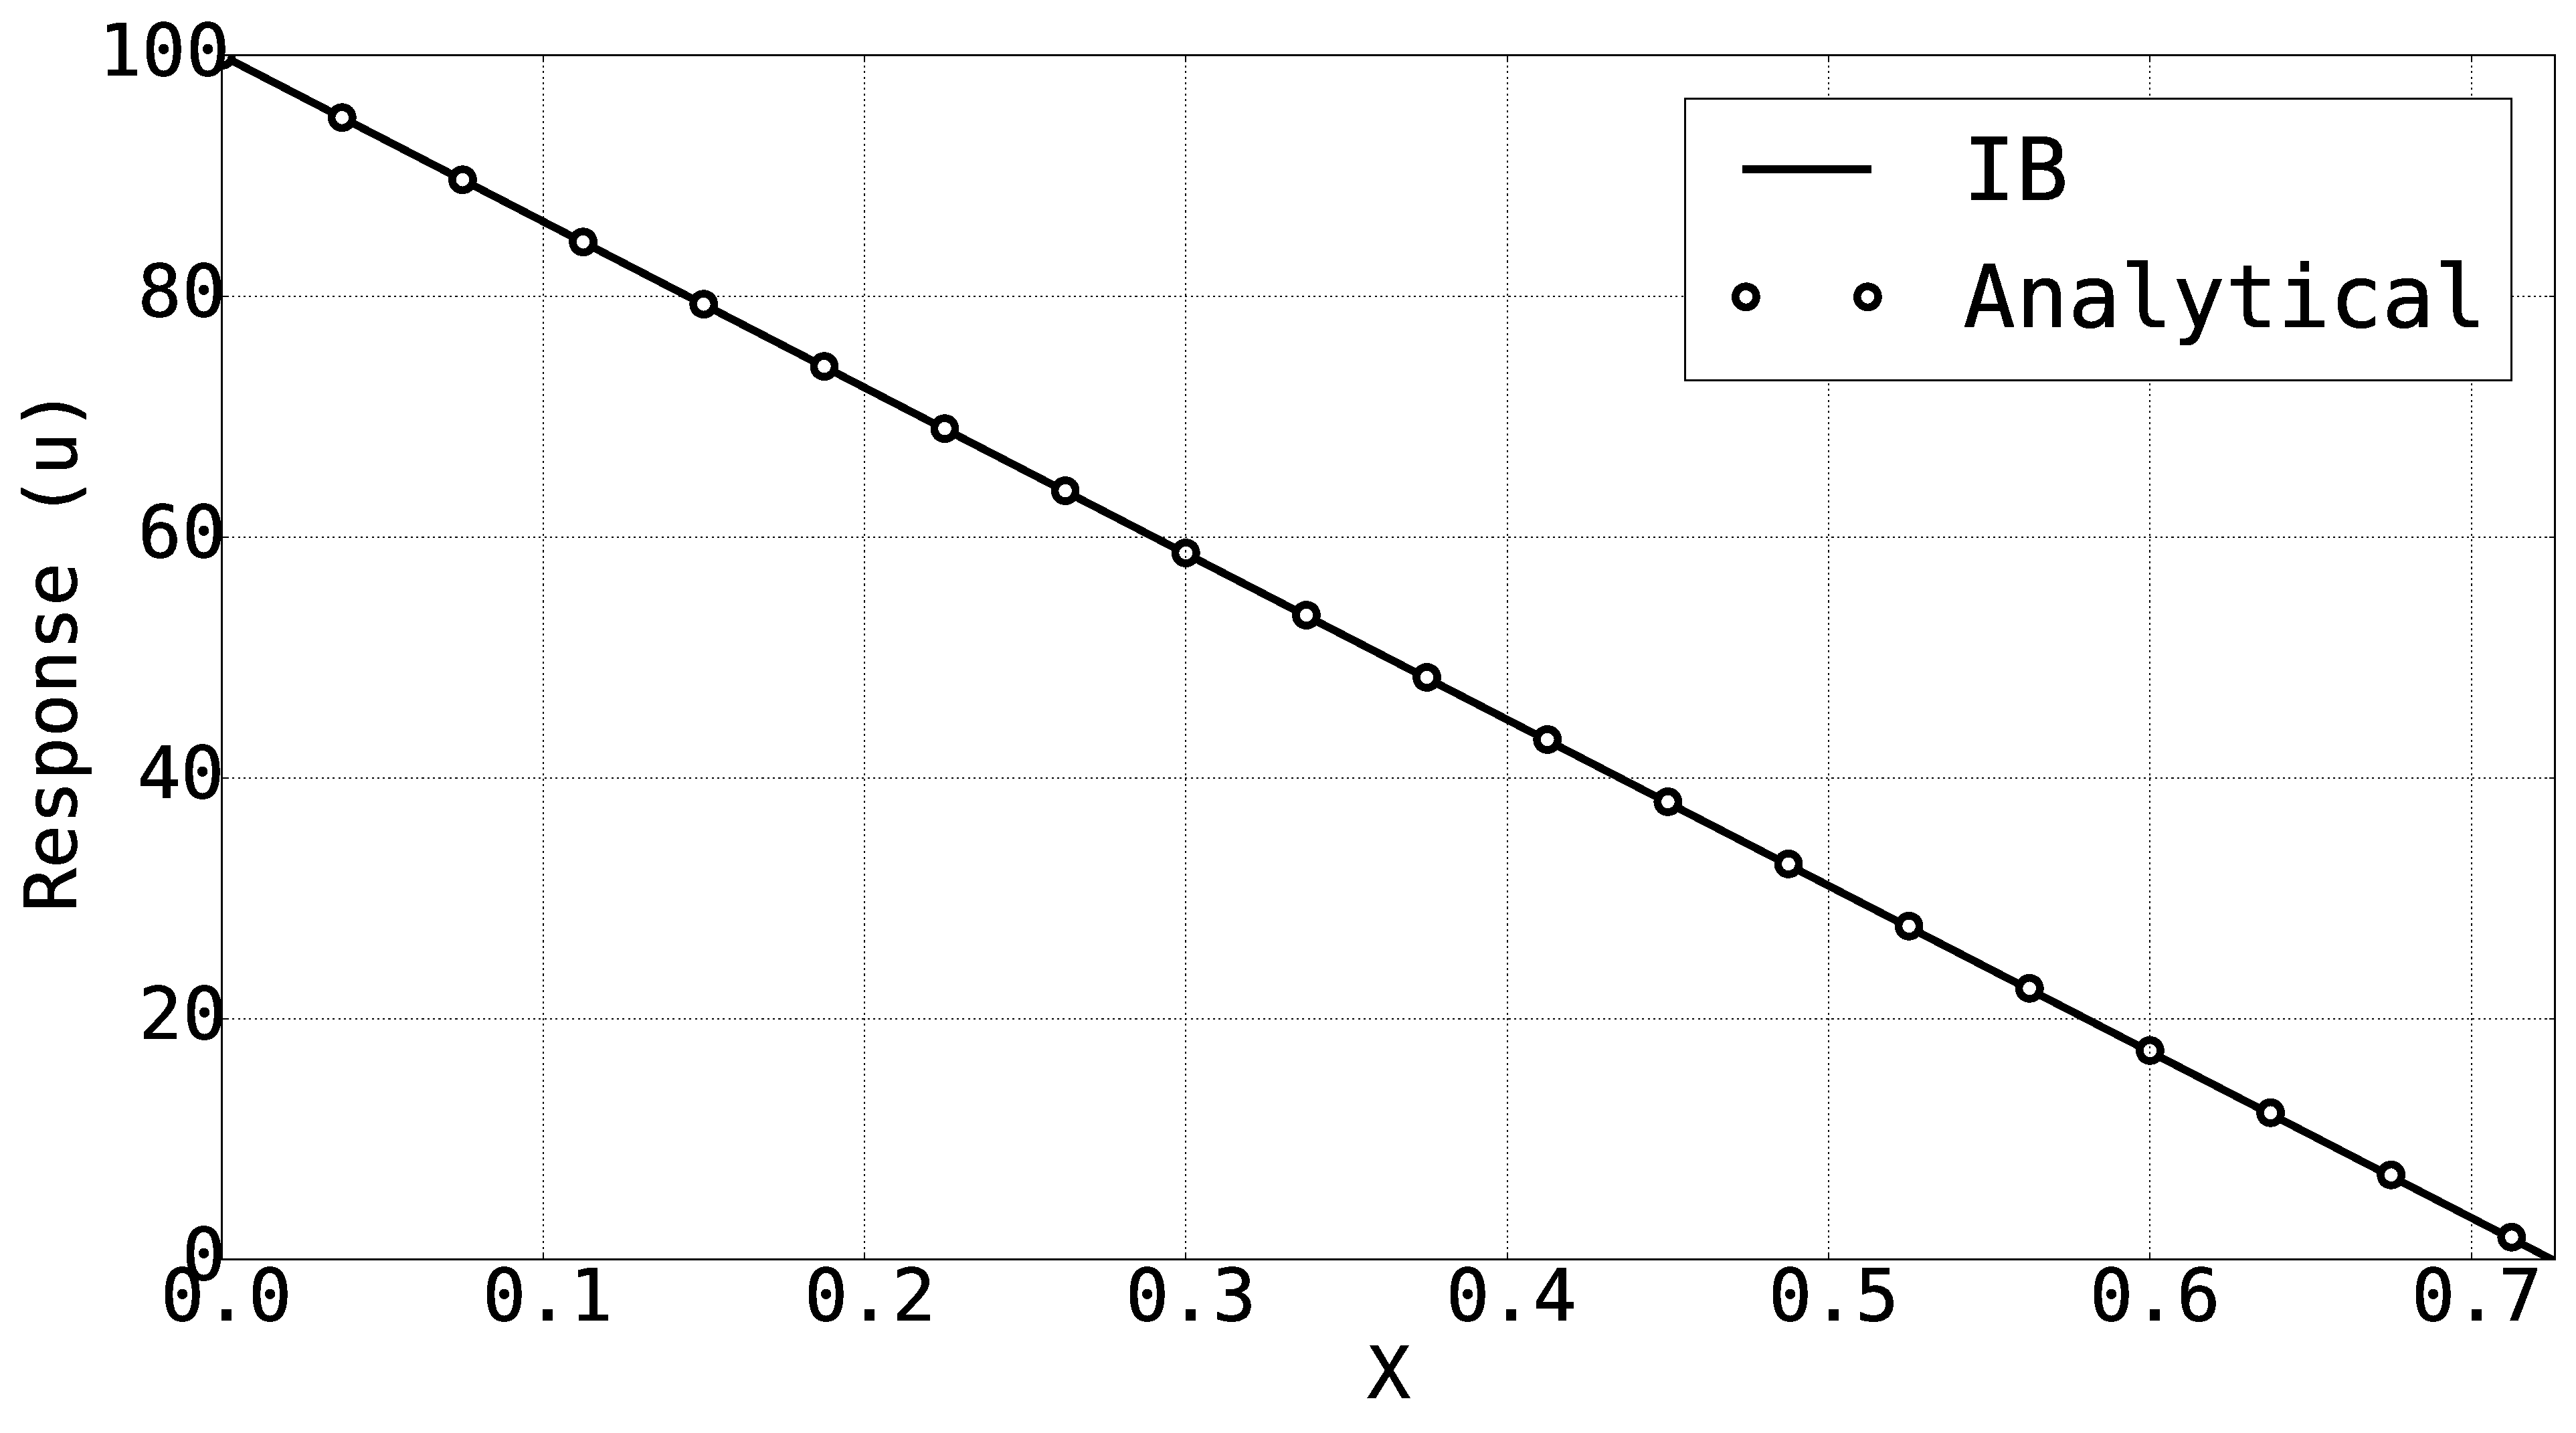
\includegraphics[width=7.0cm]{Chapter_3/figure/virtualBoundary_wallVelocity_100.eps}
	}
	\\
	\subfigure[$u_{wall} = 10^3 m/s$]
	{
	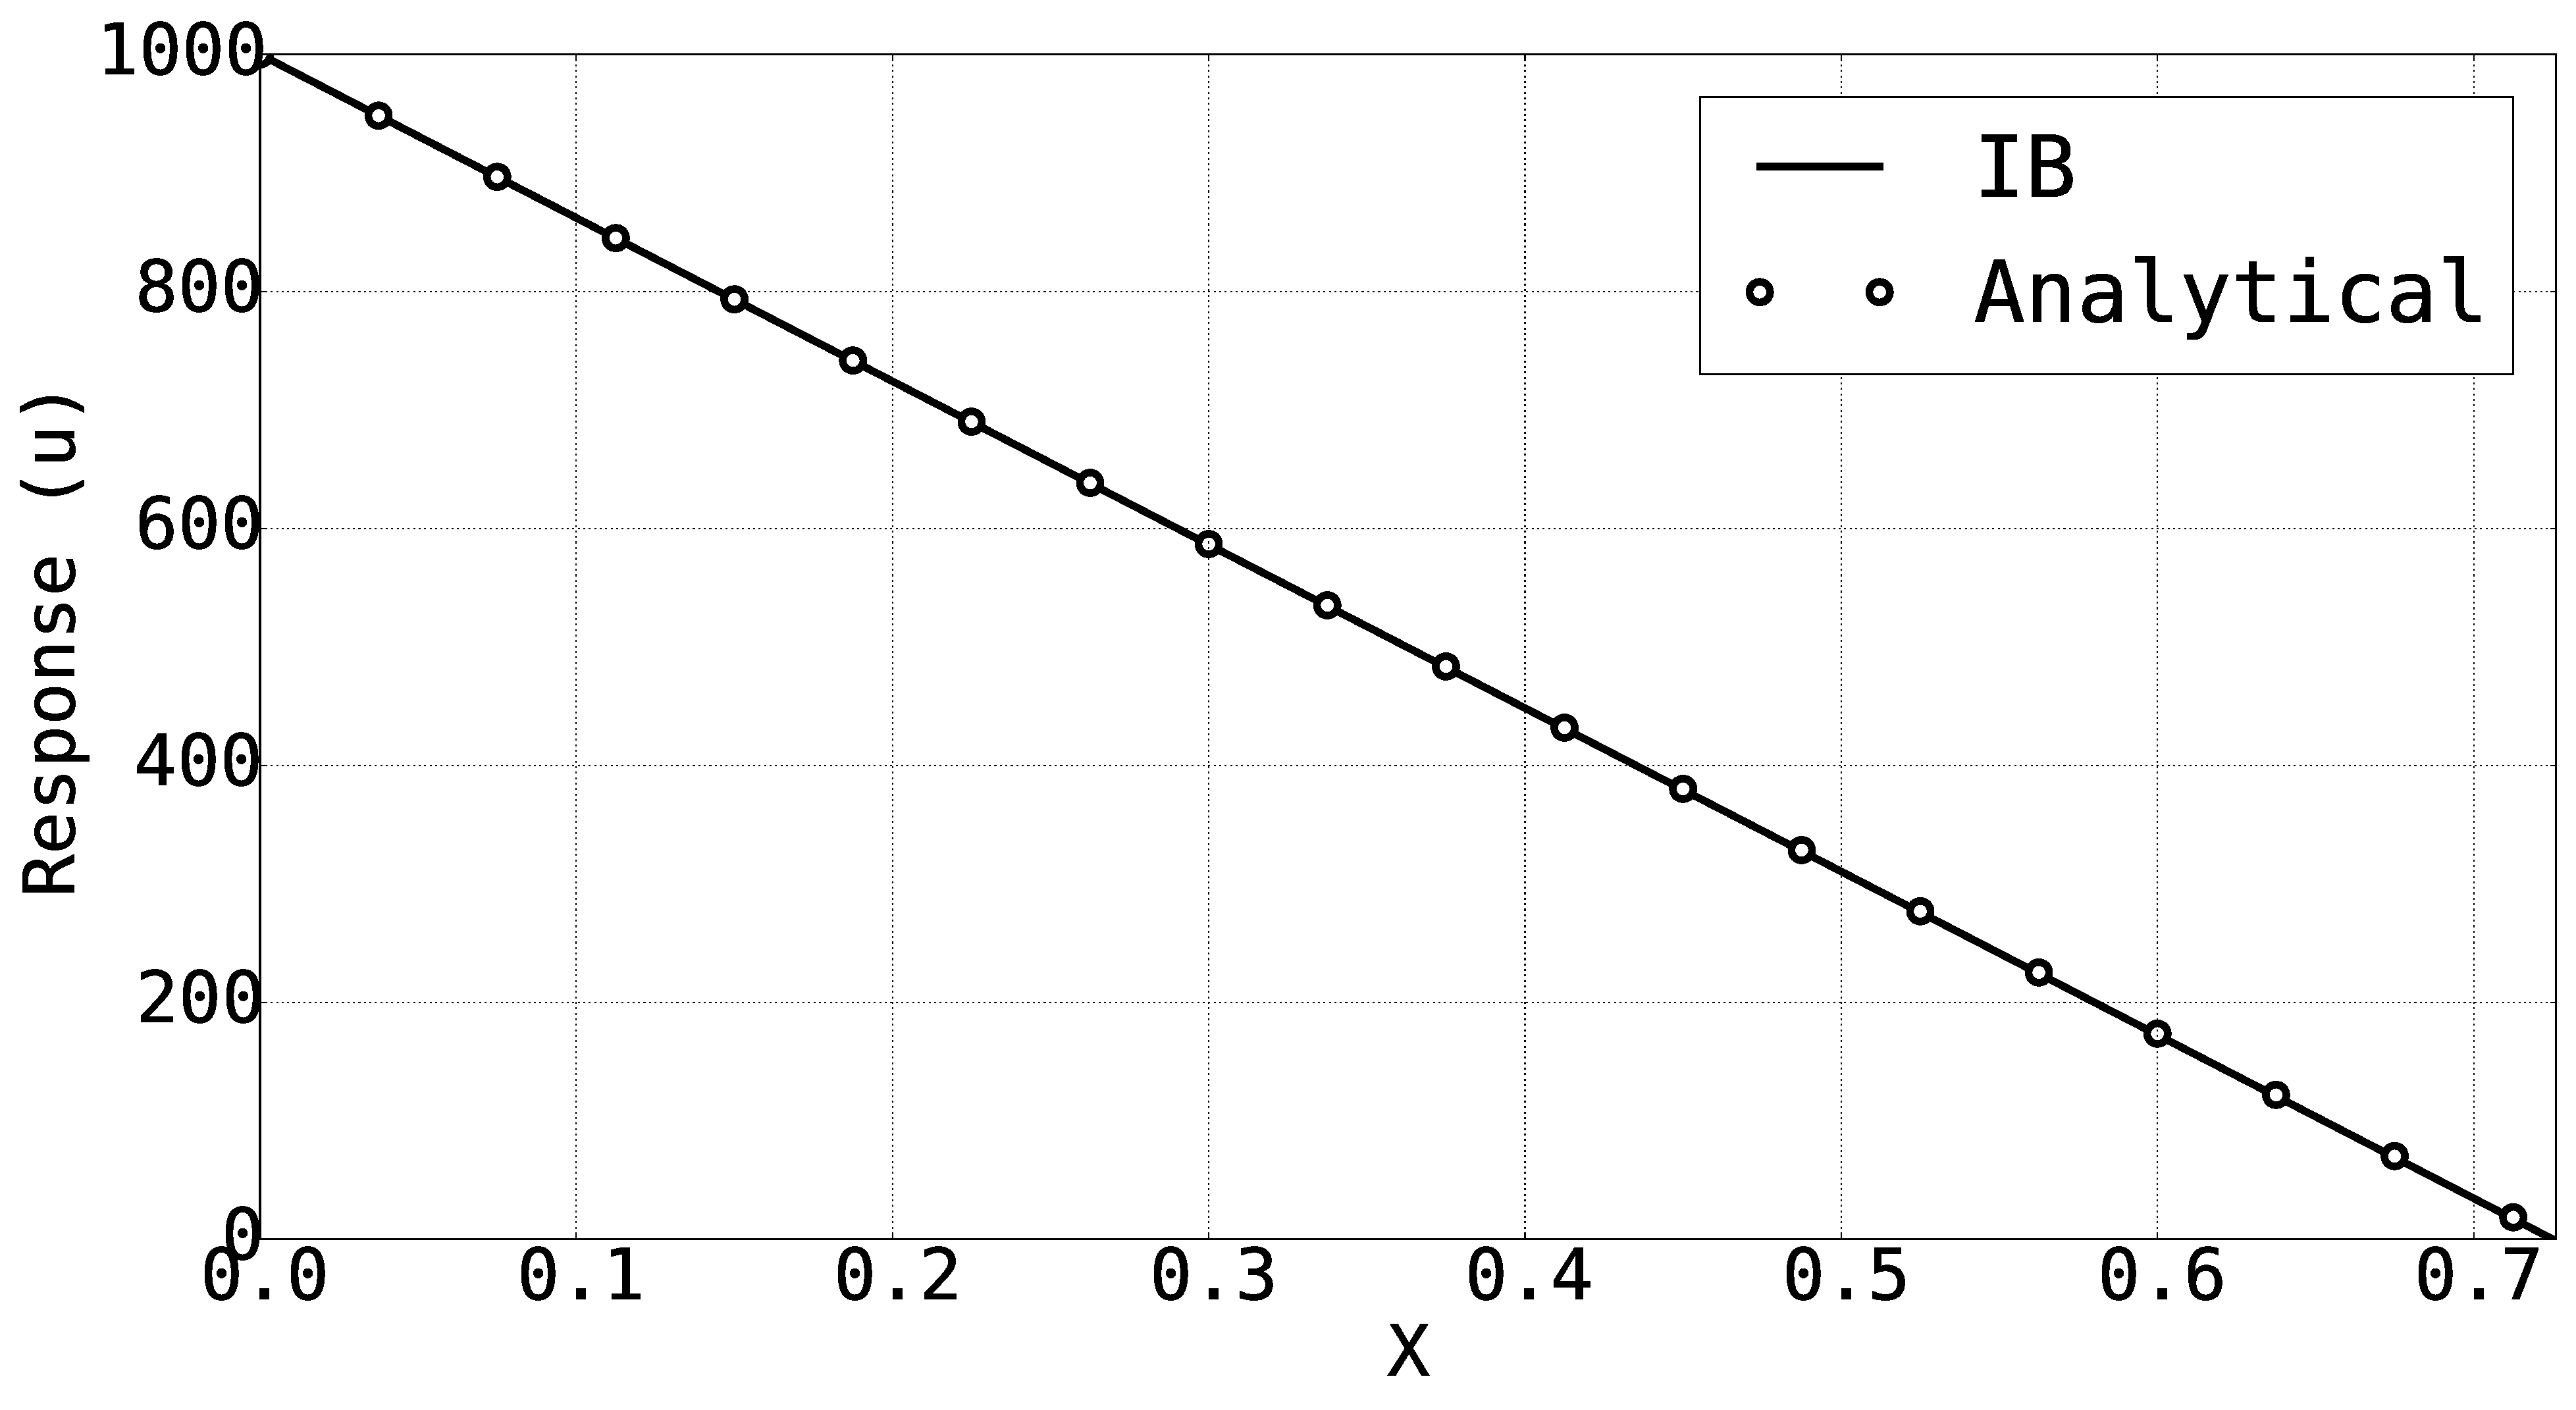
\includegraphics[width=7.0cm]{Chapter_3/figure/virtualBoundary_wallVelocity_1000.eps}
	}
	\quad
	\subfigure[$u_{wall} = 10^4 m/s$]
	{
	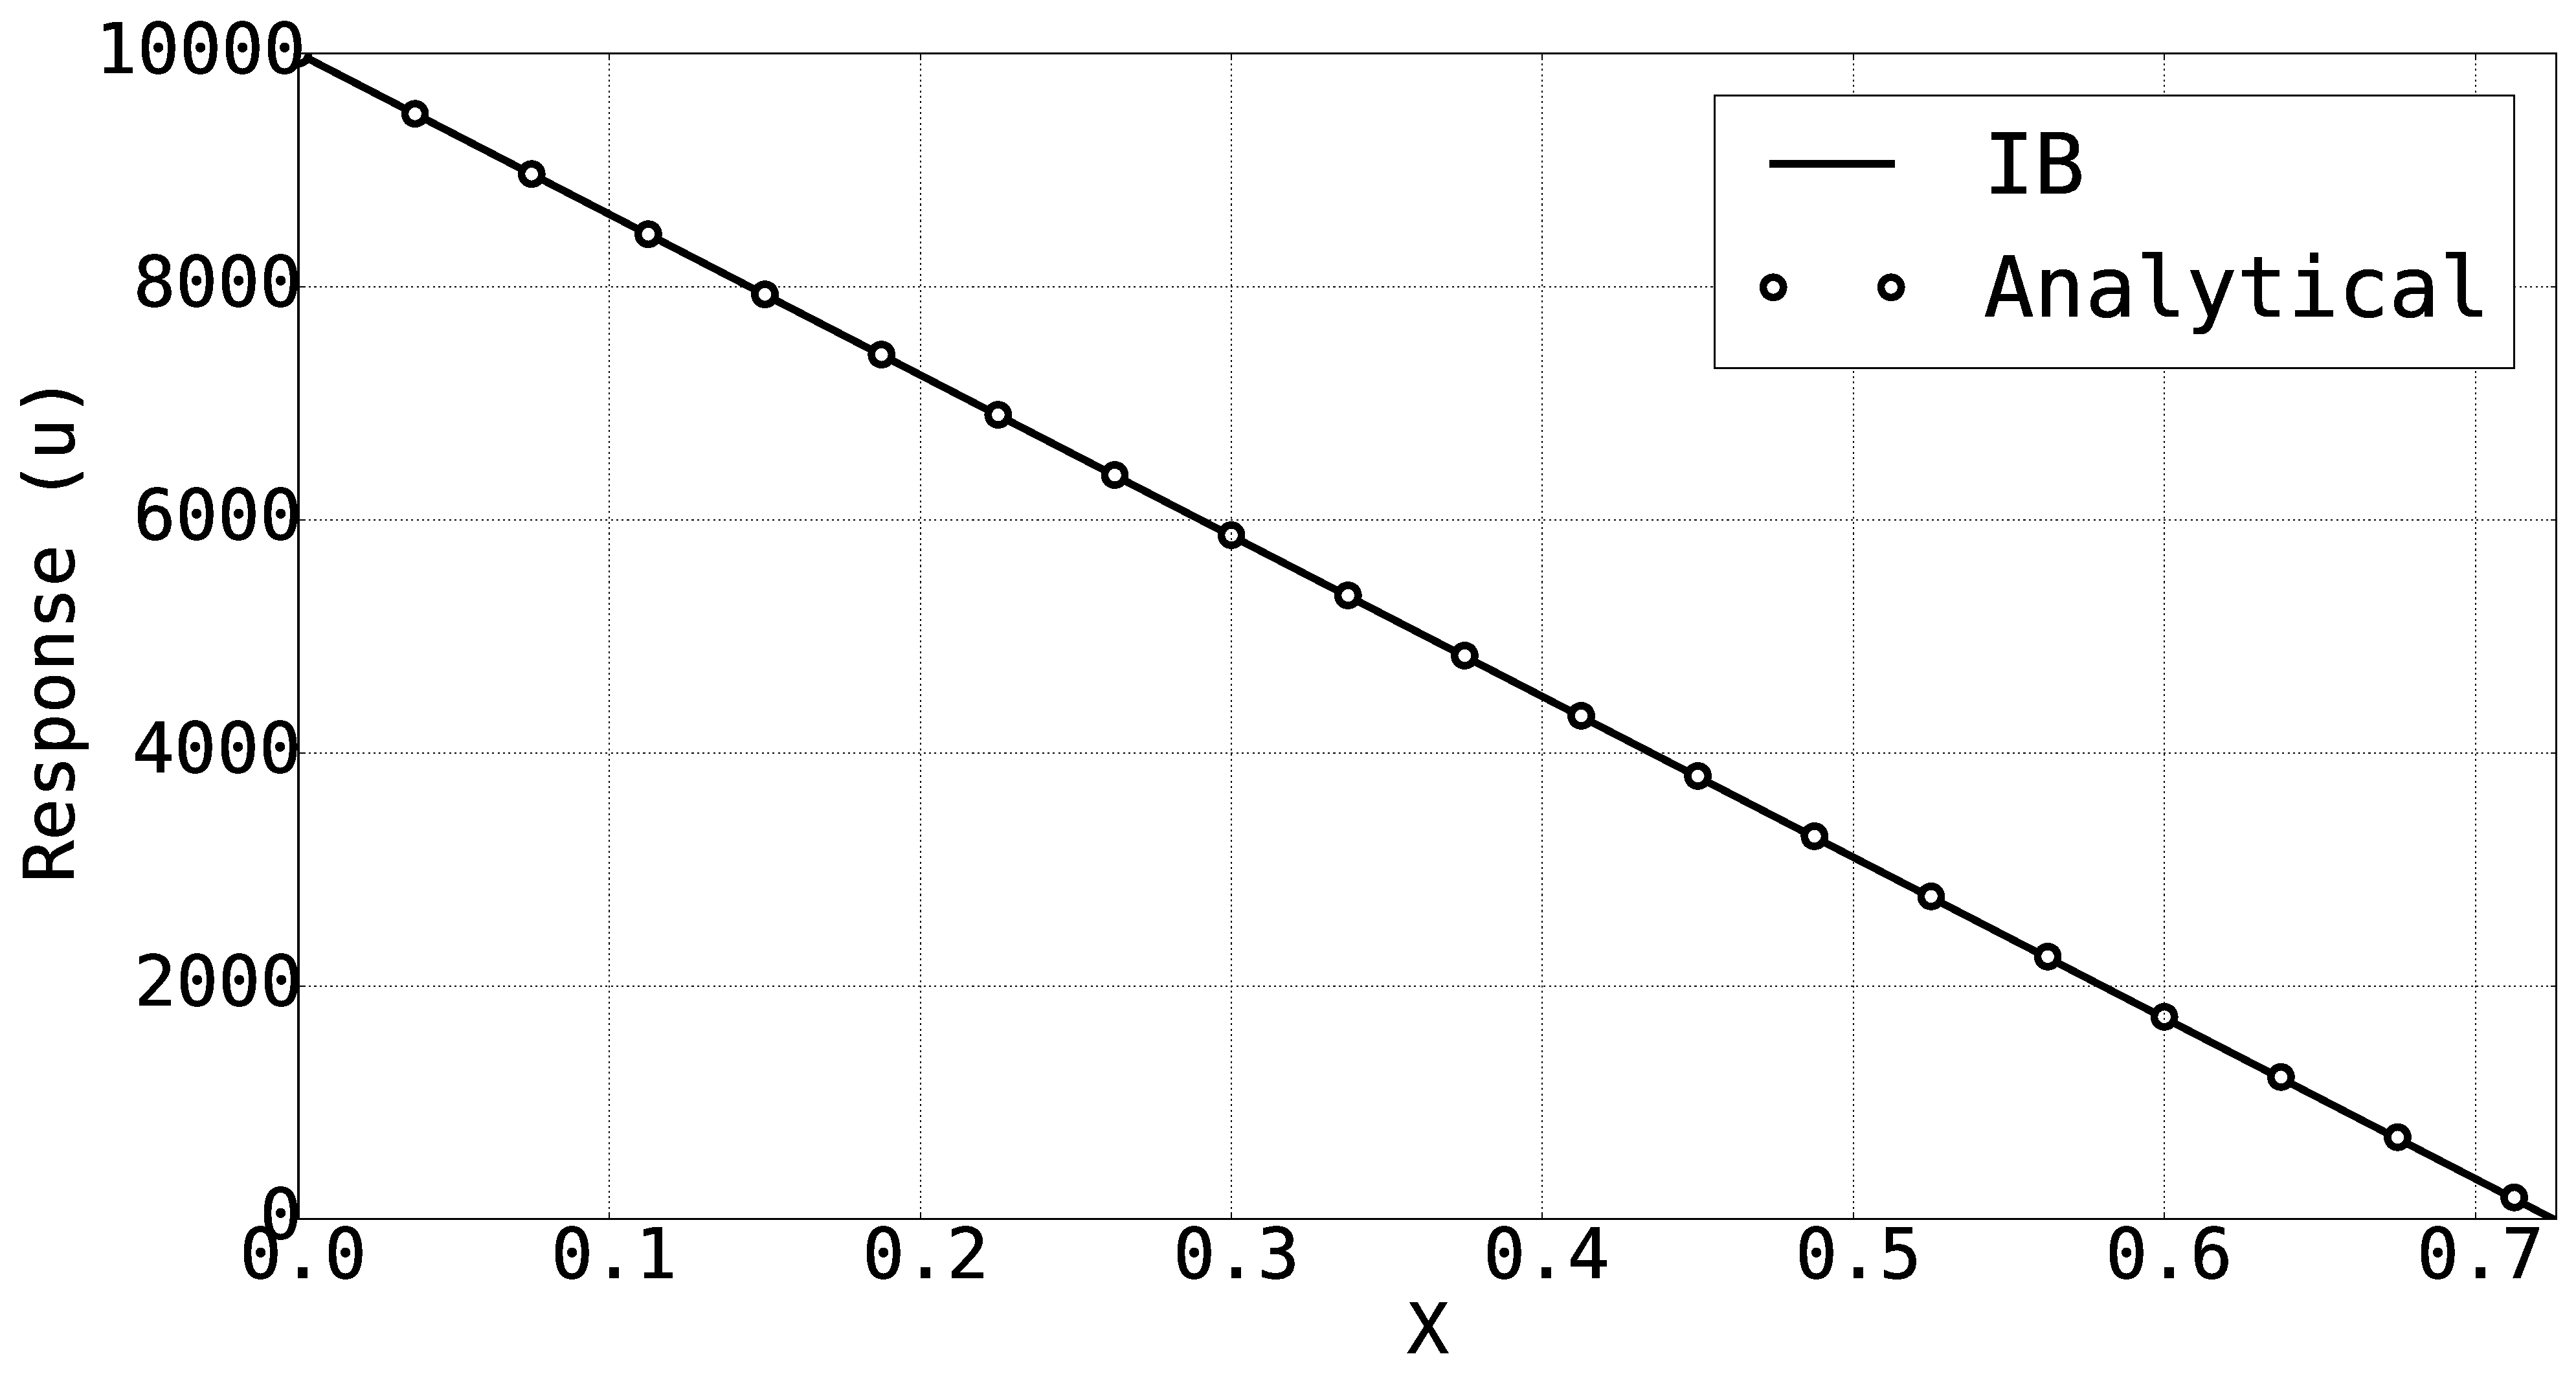
\includegraphics[width=7.0cm]{Chapter_3/figure/virtualBoundary_wallVelocity_10000.eps}
	}
	\caption{Comparison between IB and analytical results for different wall velocities.}
	\label{fig:C3_virtualBoundaryResultWallVelocity}
\end{figure}

\begin{table}[H]
\centering
\begin{tabular}{c | c}
	 Wall velocity & RMSE \\ \hline \hline
	 10 & 0.000616\\ \hline
	 $10^2$ & 0.000616 \\ \hline
	 $10^3$ & 0.000616 \\ \hline
	 $10^4$ & 0.000616 \\
\end{tabular}
\caption{RMSE value for different wall velocities.}
\label{table:C3_virtualBoundaryResultWallVelocityRMSE}
\end{table}

Finally we looked at the effect of constants $\alpha$ and $\beta$ on the accuracy of the solution. We discretized the domain using $81$ nodes with wall velocity equal to $100$ with time step equal to $10^{-5}$. The location of the fixed wall is chosen as $x_{wall} = 0.726$. The flow between the plates is modelled using different coefficients for $\alpha$ and $\beta$ as shown in Table \ref{table:C3_alphaBetaValues}.

\begin{table}[H]
\centering
\begin{tabular}{c | c | c}
	 Case number & $\alpha$ & $\beta$ \\ \hline \hline
	 1 & 10 & 0.000616\\ \hline
	 2 & $10^2$ & 0.000616 \\ \hline
	 3 & $10^3$ & 0.000616 \\ \hline
	 4 & $10^4$ & 0.000616 \\
\end{tabular}
\caption{RMSE value for different wall velocities.}
\label{table:C3_alphaBetaValues}
\end{table}
% -.-.-.-.-.-.-.-.-.-.-.-.-.-.-.-.-.-.-.-.-.-.-.-.-.-.-.-.-.-.-.-.-.-
\subsection{Penalization method}
The third class of continuum immersed boundary techniques are known as penalization method that was first introduced by Arquis and Caltagirone \cite{ arquis1984conditions}. In this method, the solid boundaries are modeled as porous media. Porosity or void fraction is a measure of the void spaces in a material, and is a fraction of the volume of voids over the total volume, between 0 and 1. For the solid domain the porosity value is near zero whereas for the fluid domain its value is close to one. Flow through a porous domain is described using the Darcy's law. This is a simple proportional relationship between the instantaneous discharge rate through a porous medium, the viscosity of the fluid and the pressure drop over a given distance.

\begin{figure}[H]
	\centering
	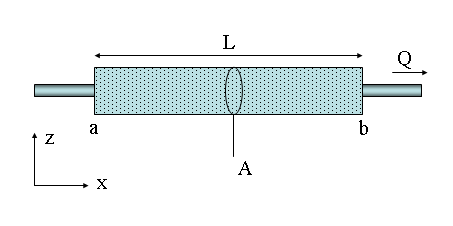
\includegraphics[width=14.cm]{Chapter_3/figure/Darcys_Law.png}
	\caption{Flow through a porous pipe.}
\end{figure}

For a flow through a porous domain in a pipe shown in Figure \ref{fig:C3_darcyEquationPipe}, Darcy's law is written as

\begin{equation}\label{eq:C3_DarcysLaw}
	Q = \frac{\kappa A \Delta p}{\mu L}
\end{equation}

where $Q$ is the total flow discharge, $\kappa$ is the permeability of the domain, $\Delta p$ is the pressure drop due to the porosity between two ends of the pipe, $\mu$ is the fluid's viscosity, and $L$ is the length of the domain. Darcy's law can be considered as a relation between the flow velocity and pressure drop. This pressure drop  is used in the penalization method to represent the solid boundaries by modelling the force term using Equation \eqref{eq:C3_DarcysLaw}. The force term is defined as follows

\begin{equation}\label{eq:C3_forceTermIBpenelization}
	f = - \mathcal{H}(\mathcal{X}) \frac{\mu}{\kappa} v
\end{equation}

where $v$ is is the velocity of the flow. In order to apply the force term only to the region inside the the solid boundary, the penalization force is multiplied by a Heaviside function, $\mathcal{H}(\mathcal{X})$, that is a function of relative distance of the points in the domain to the boundary of the solid region. The Heaviside function $\mathcal{H}$ has the value of \emph{one} for all points inside the solid boundary and is \emph{zero} for points outside the boundary. This will give us a zero forcing term for points outside the solid boundary and non-zero for points inside. Therefore, the pressure drop is only applied to the points inside the solid domain. This is explained in more details in the following example.

Assume that the solid boundary is a circle, located at $(1,2)$ with a radius of $2$. This curve is defined using the following equation.

\begin{equation}
	(x - 1)^2 + (y - 2)^2 = 4
\end{equation}

The relative location of an arbitrary point $x_0 = (\eta, \rho)$ with respect to this boundary is defined using the following equation

\begin{equation}
	\mathcal{X}(\eta, \rho) = 4 - (\eta - 1)^2 - (\rho - 2)^2
\end{equation}

Depending of the sign of $\mathcal{X}$, we can make the following conclusions

\begin{equation}
\begin{cases}
	\mathcal{X} > 0 \quad \text{$x_0$ is inside the solid boundary} \\
	\mathcal{X} < 0 \quad \text{$x_0$ is outside the solid boundary} \\
	\mathcal{X} = 0 \quad \text{$x_0$ is on the boundary}
\end{cases}
\end{equation}

Sign of $\mathcal{X}$ divides the physical domain into three regions. To use this function for force term assignment to mesh cell, we need to convent its values to $0$ and $1$. The force terms outside the solid boundaries are multiplied by zero whereas the force terms inside the solid boundary are multiplied by one. This is done by feeding the values of function $\mathcal{X}$ to a Heaviside function, $\mathcal{H}$. The Heaviside function, or the unit step function, is a discontinuous function whose value is zero for negative argument and one for positive argument as shown in Figure \ref{fig:C3_heavisideFunction}.

\begin{figure}[H]
	\centering
	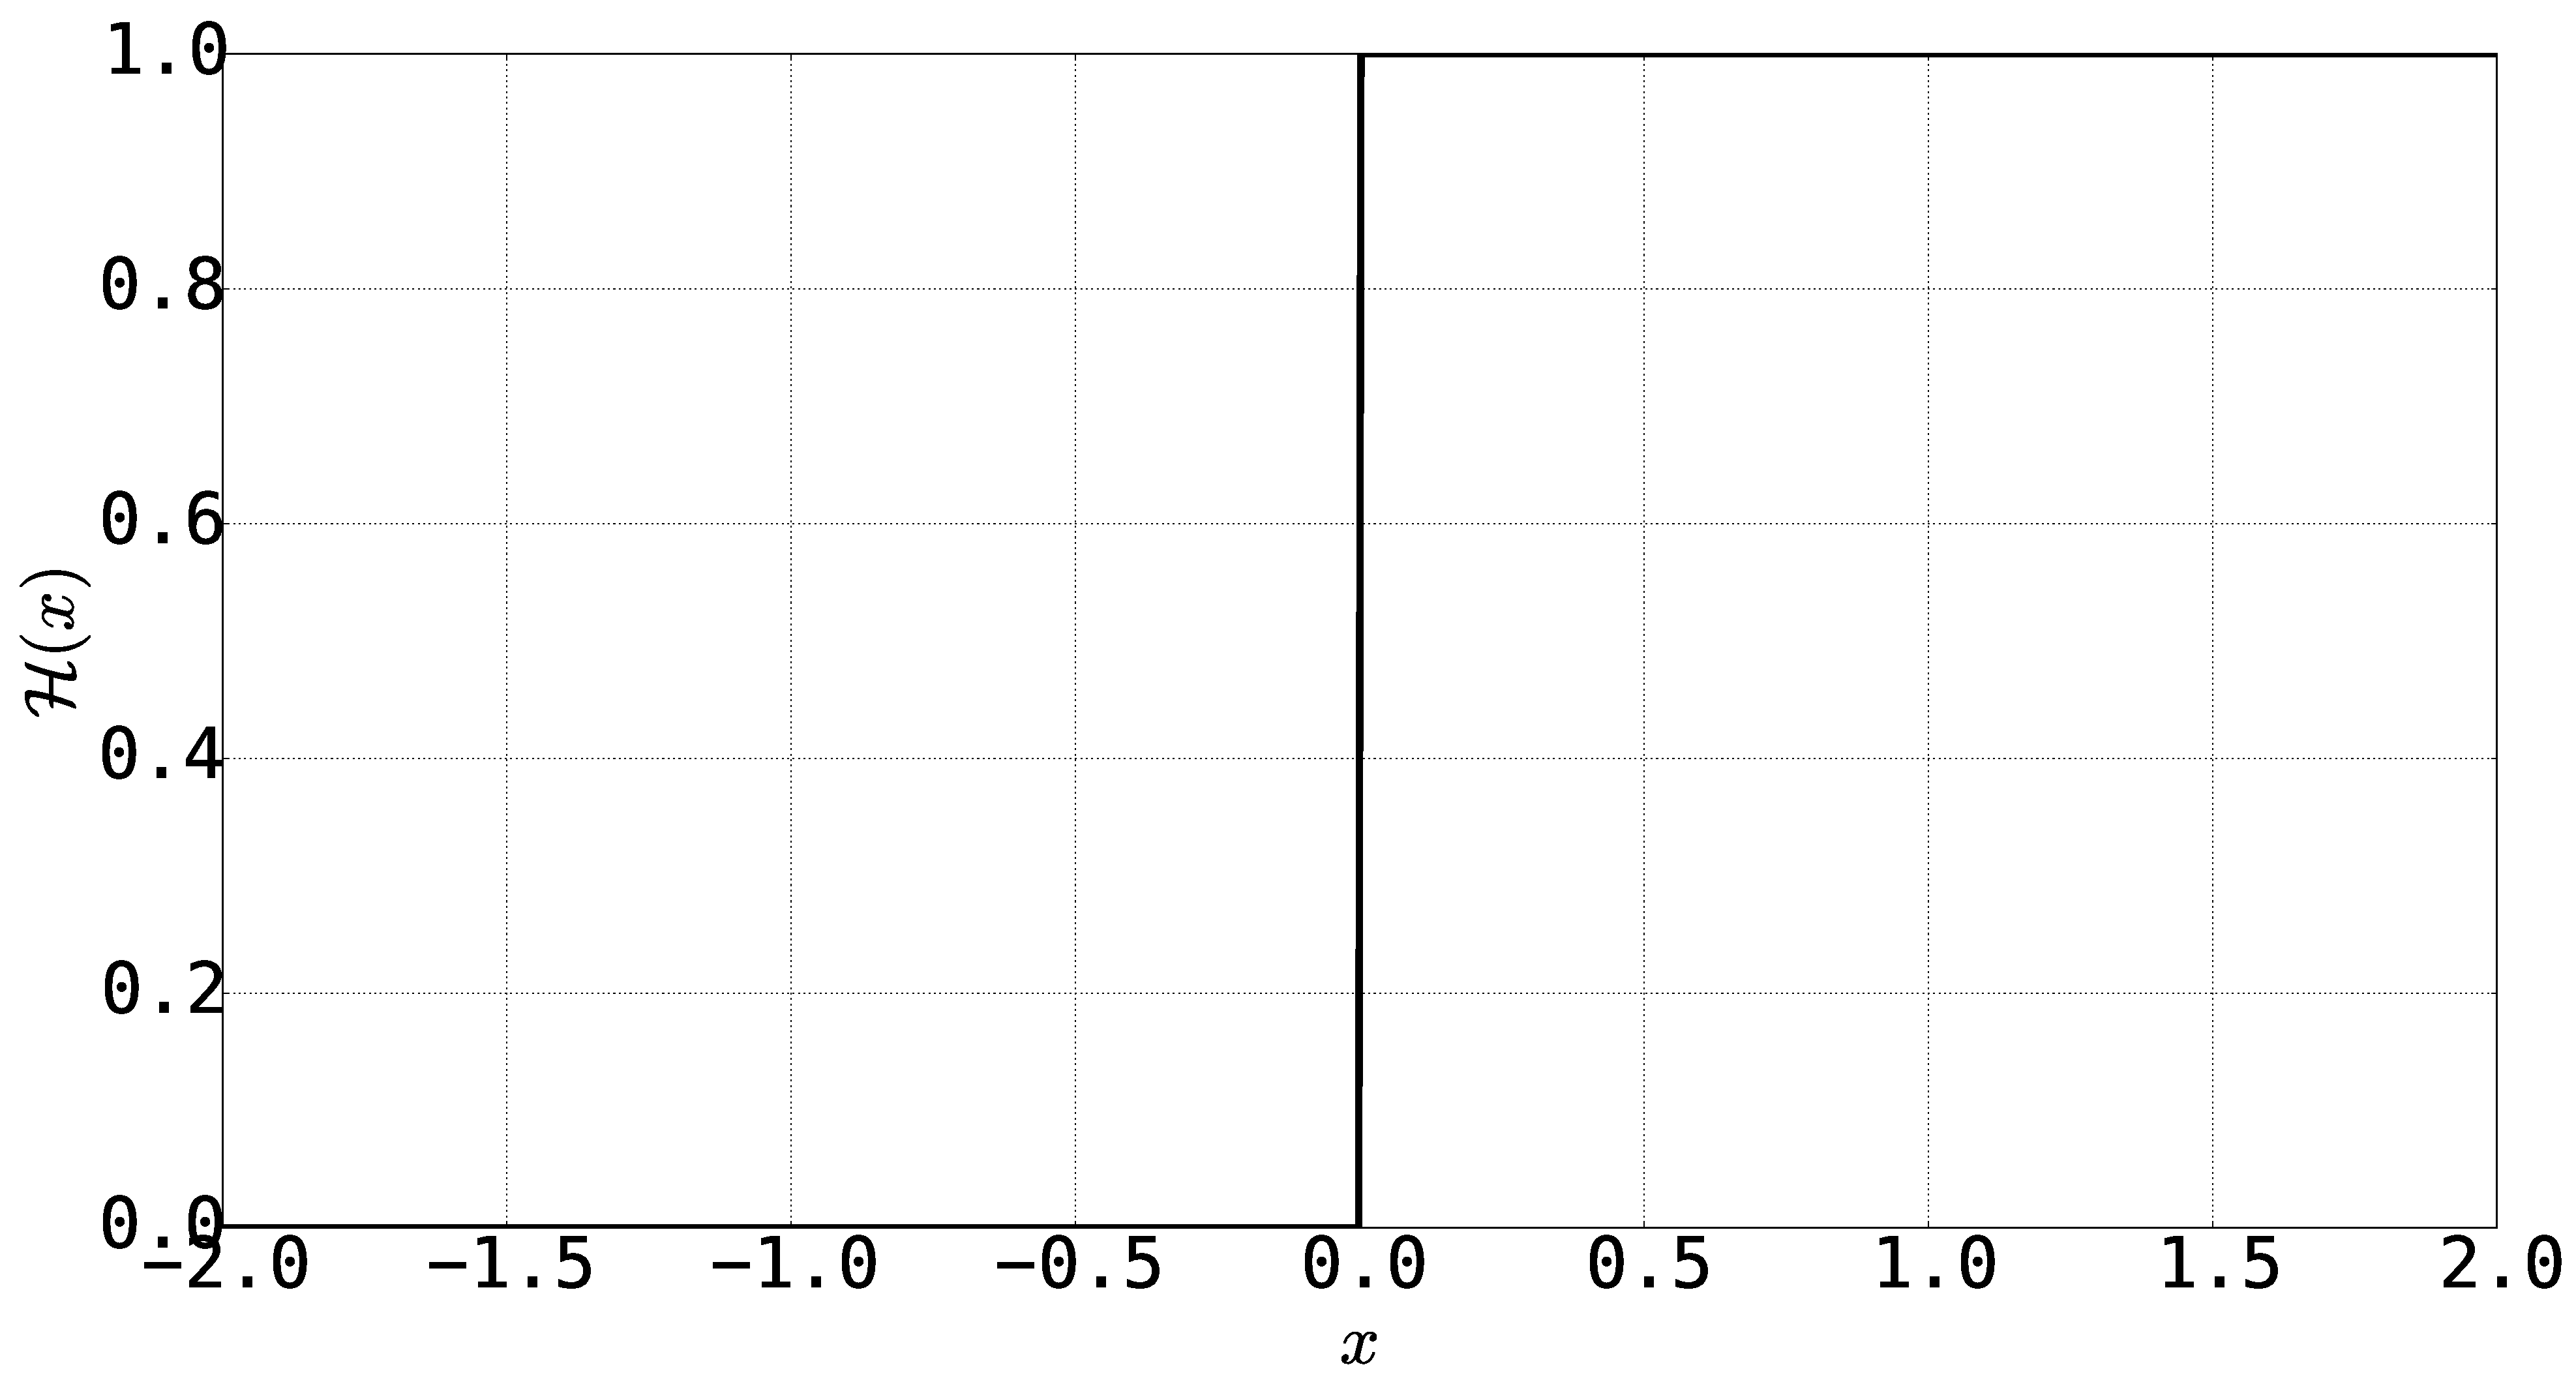
\includegraphics[width=14.cm]{Chapter_3/figure/Heaviside_Function.eps}
	\caption{The Heaviside function.}
	\label{{fig:C3_heavisideFunction}}
\end{figure}

By feeding the function $\mathcal{X}$ into the Heaviside function, we get the value of one for nodes inside the solid boundary and zero for outside. These are then multiplied to the force terms calculated using Equation \eqref{eq:C3_forceTermIBpenelization}. This enables us to apply the force term only within the solid domain. This method is applied to the demonstration problem of section \ref{sec:C3_benchmark_case}. For this problem, we looked at the effect of the number of mesh cells, wall velocity, and the permeability value on the accuracy of the method. The results are compared with analytical results for this problem like the previous sections.

For the first set of results, we looked at the effect of mesh size on the accuracy of the solution. The domain length is chosen as $1.0 m$ where the position of the fixed wall is selected as $0.6125$. We chose this so that the computational nodes won't coincide the with the wall location. This better represents the application of the IB method. We chose the node numbers as 11, 41, 81, and 161. As shown in Figure \ref{fig:C3_penalizationResultNodeNumber}, as we increase the number of the total error between the numerical and analytical results decreases. For the Case where there is computational node exactly on top the location for the stationary wall ($n=161$), the two results match perfectly. The IB results are shown using solid line and the analytical results are represented using white circles.

\begin{figure}[H]
	\centering
	\subfigure[n = 11]
	{
	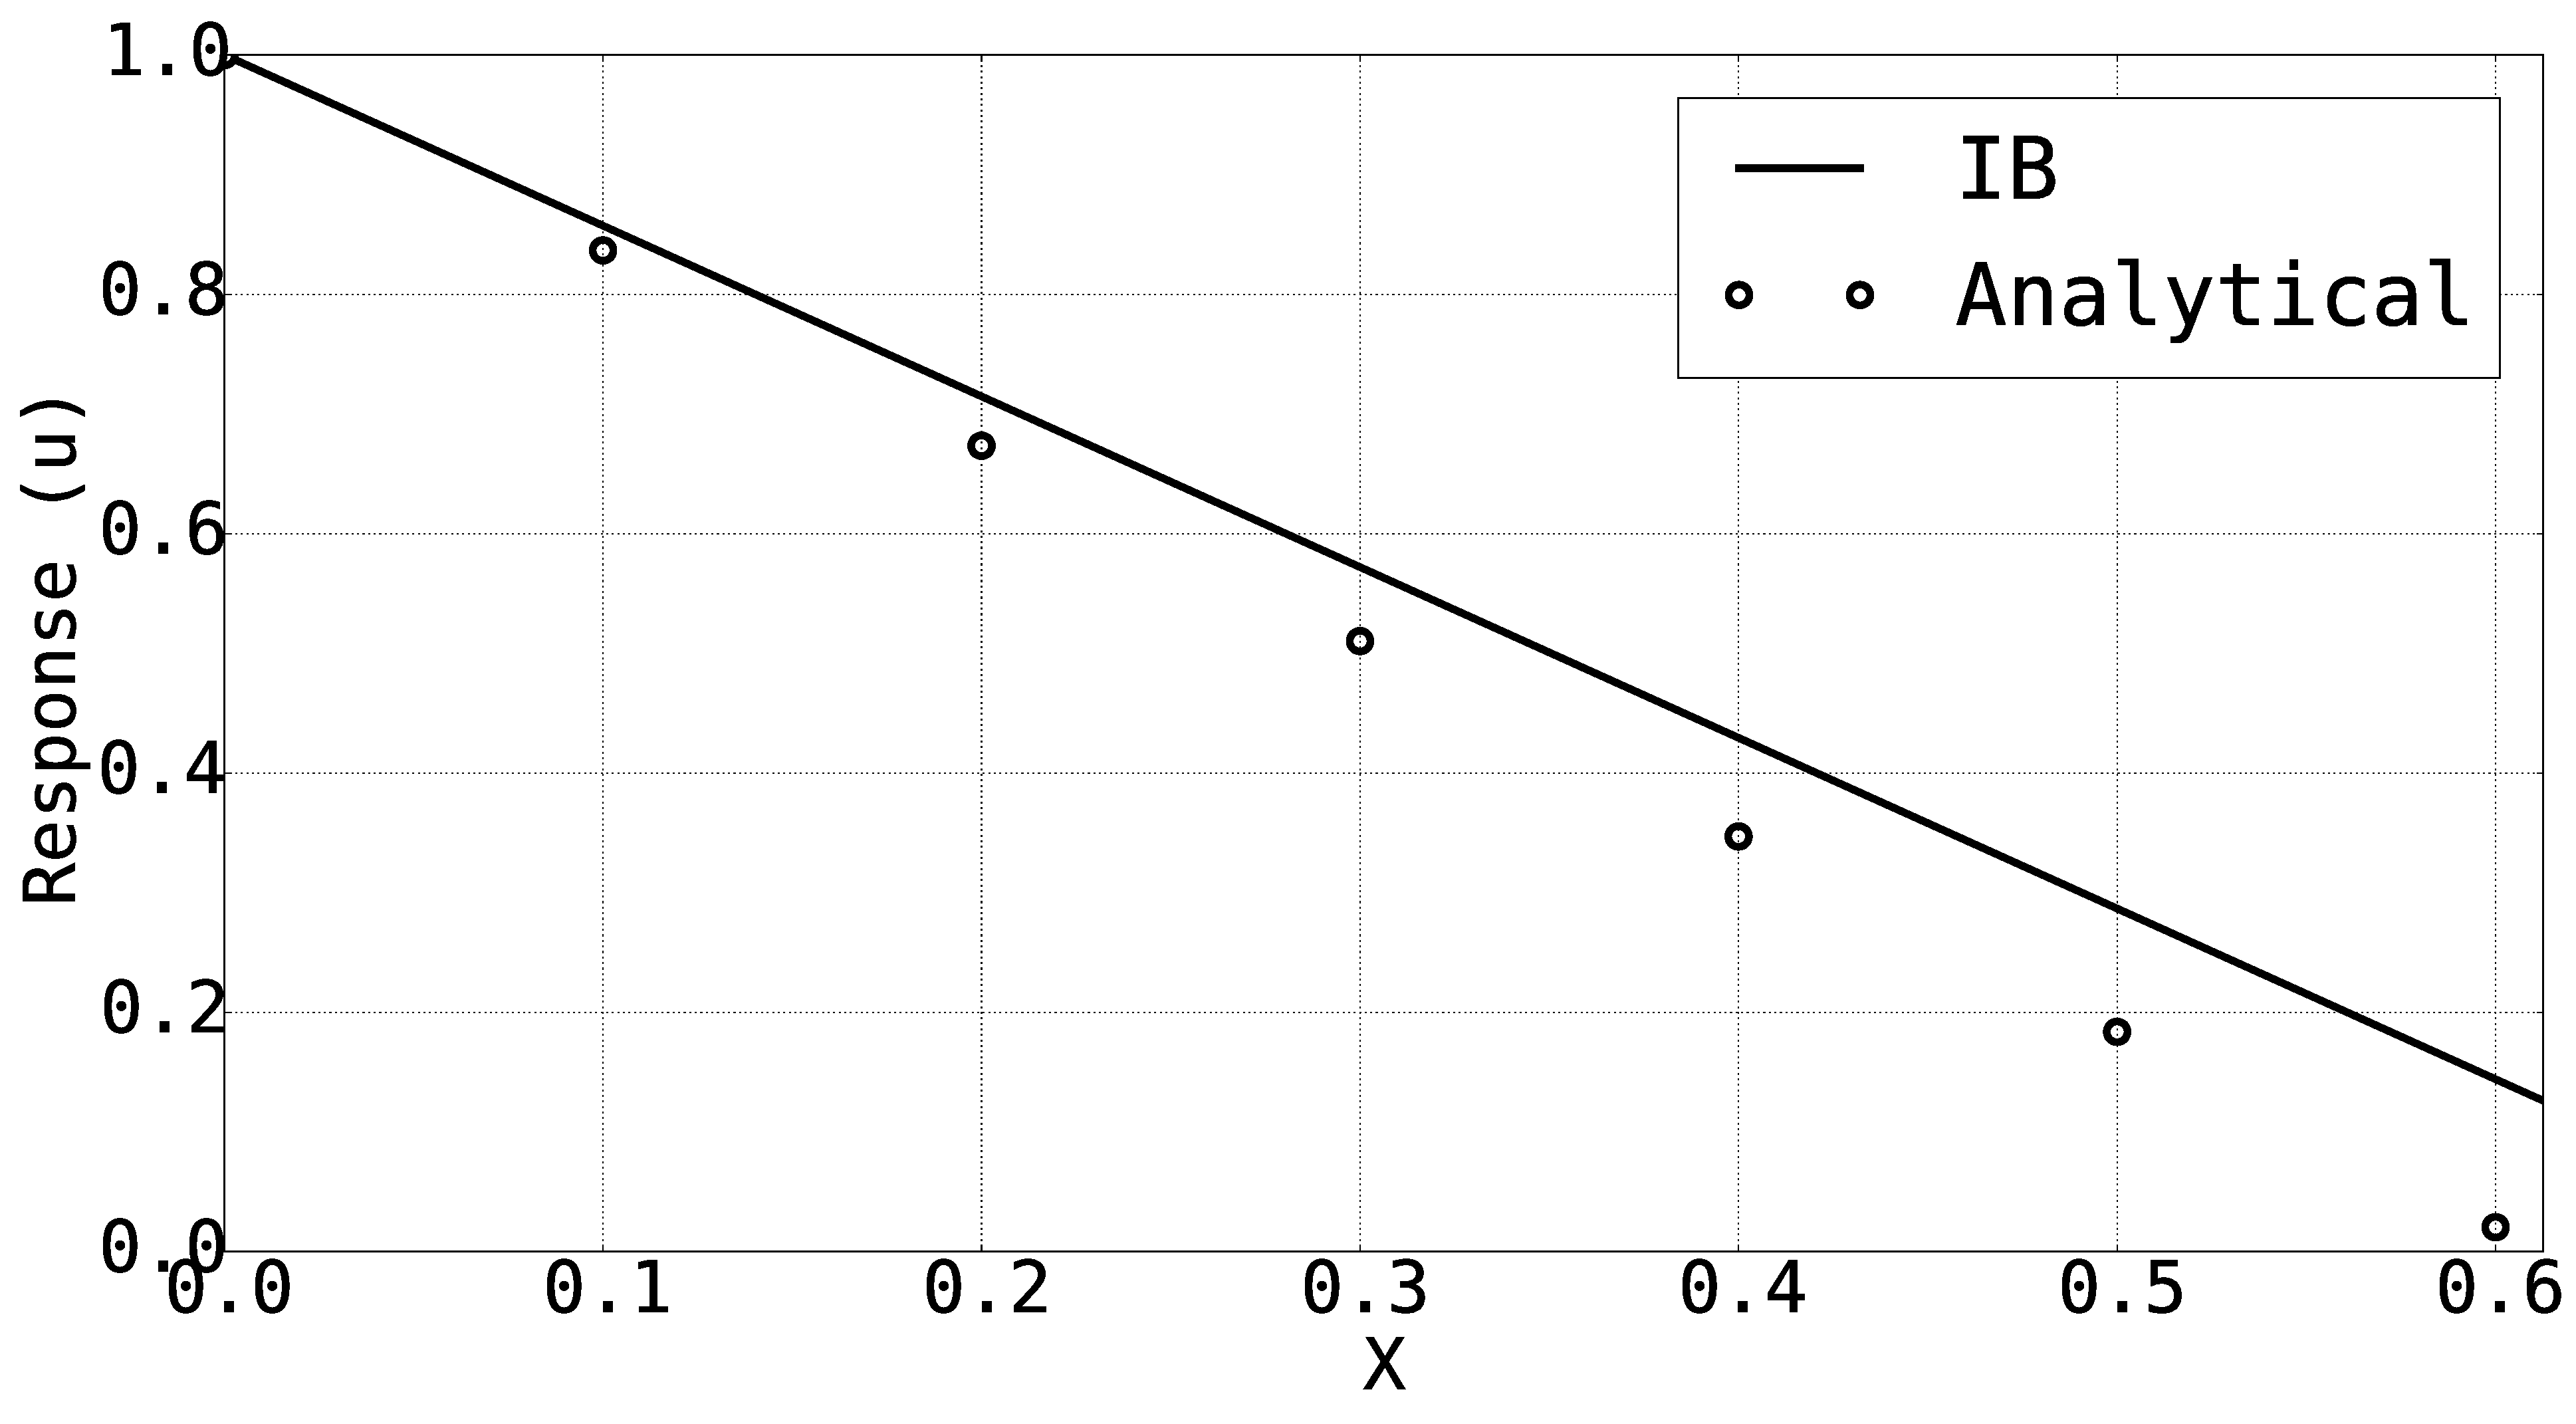
\includegraphics[width=7.0cm]{Chapter_3/figure/penalization_nodeNumber_11.eps}
	}
	\quad
	\subfigure[n = 41]
	{
	\includegraphics[width=7.0cm]{Chapter_3/figure/penalization_nodeNumber_41.eps}
	}
	\\
	\subfigure[n = 81]
	{
	\includegraphics[width=7.0cm]{Chapter_3/figure/penalization_nodeNumber_81.eps}
	}
	\quad
	\subfigure[n = 161]
	{
	\includegraphics[width=7.0cm]{Chapter_3/figure/penalization_nodeNumber_161.eps}
	}
	\caption{Comparison between IB and analytical results for different number of nodes.}
	\label{fig:C3_penalizationResultNodeNumber}
\end{figure}

For the comparison between the IB and the analytical results we used the RSME value. These are shown in Table \ref{table:C3_penalizationResultNodeNumberRMSE}.

\begin{table}[H]
\centering
\begin{tabular}{c | c}
	Node number & RMSE value \\ \hline \hline
	11 & 0.0624 \\ \hline
	41 & 0.0139 \\ \hline
	81 & 0.005 \\ \hline
	161 & 0.001
\end{tabular}
\caption{RMSE value for different number of nodes}
\label{table:C3_penalizationResultNodeNumberRMSE}
\end{table}

As can be seen in Table \ref{table:C3_penalizationResultNodeNumberRMSE}, even for $n = 161$, the RMSE value is not zero. This is because in the penalization method, even for low values of porosity, there is still a small flow going through the solid domain.

For the next investigation, we look at the effect of the different velocity of moving wall on the accuracy of the penalization method. For this analysis we defined the fixed wall at $x=0.4325$ and discretized the domain using $81$ nodes. The inlet velocity is selected as $1$, $10$, $100$, and $1000$. To verify the methodology, we compared the IB with analytical results. We chose the time step as $10^{-5}$ and the porosity value as $\kappa = 10^{-5}$. As shown in Figure \ref{fig:C3_penalizationResultInletVelocity} and the RMSE values in Table \ref{table:C3_penalizationResultInletVelocityRMSE}, the inlet velocity does not affect the the accuracy of the response. Moreover, all of these simulation are done using the same time step and porosity value.

\begin{figure}[H]
	\centering
	\subfigure[$U_{in} = 1 m/s$]
	{
	\includegraphics[width=7.0cm]{Chapter_3/figure/penalization_inletVelocity_1.eps}
	}
	\quad
	\subfigure[$U_{in} = 10 m/s$]
	{
	\includegraphics[width=7.0cm]{Chapter_3/figure/penalization_inletVelocity_10.eps}
	}
	\\
	\subfigure[$U_{in} = 100 m/s$]
	{
	\includegraphics[width=7.0cm]{Chapter_3/figure/penalization_inletVelocity_100.eps}
	}
	\quad
	\subfigure[$U_{in} = 1000 m/s$]
	{
	\includegraphics[width=7.0cm]{Chapter_3/figure/penalization_inletVelocity_1000.eps}
	}
	\caption{Comparison between IB and analytical results for different inlet velocity.}
	\label{fig:C3_penalizationResultInletVelocity}
\end{figure}

\begin{table}[H]
\centering
\begin{tabular}{c | c}
	Inlet velocity (m/s) & RMSE value \\ \hline \hline
	1 & 0.0056 \\ \hline
	10 & 0.0056 \\ \hline
	100 & 0.0056 \\ \hline
	1000 & 0.0056
\end{tabular}
\caption{RMSE value for different inlet velocities.}
\label{table:C3_penalizationResultInletVelocityRMSE}
\end{table}

Finally, we looked at the effect of different porosity values on the accuracy of the simulation. For this purpose, we fixed the wall location at $x_{wall} = 0.435$ and defined the velocity of the moving wall as $10 m/s$. The length of the domain is selected as $1 m$ and discretized using 81 nodes. We chose the time step as $10^{-5}$. We investigated the accuracy of penalization method to porosity values of $10^{-2}$, $10^{-3}$, $10^{-4}$, $10^{-5}$ by comparing the IB simulation with analytical results. The results shown in Figure \ref{fig:C3_penalizationResultPorosity} and Table \ref{table:C3_penalizationResultPorosityRMSE} shows the strong dependency of the simulation results of the porosity, $\kappa$, value. To select an appropriate porosity, several simulations need to be run and the convergence needs to be studied.

\begin{figure}[H]
	\centering
	\subfigure[$\kappa = 10^{-2}$]
	{
	\includegraphics[width=7.0cm]{Chapter_3/figure/penalization_porosity_100.eps}
	}
	\quad
	\subfigure[$\kappa = 10^{-3}$]
	{
	\includegraphics[width=7.0cm]{Chapter_3/figure/penalization_porosity_1000.eps}
	}
	\\
	\subfigure[$\kappa = 10^{-4}$]
	{
	\includegraphics[width=7.0cm]{Chapter_3/figure/penalization_porosity_10000.eps}
	}
	\quad
	\subfigure[$\kappa = 10^{-5}$]
	{
	\includegraphics[width=7.0cm]{Chapter_3/figure/penalization_porosity_100000.eps}
	}
	\caption{Comparison between IB and analytical results for different porosity values.}
	\label{fig:C3_penalizationResultPorosity}
\end{figure}

\begin{table}[H]
\centering
\begin{tabular}{c | c}
	Porosity (m/s) & RMSE value \\ \hline \hline
	$10^{-2}$ & 0.079 \\ \hline
	$10^{-3}$ & 0.028 \\ \hline
	$10^{-4}$ & 0.01 \\ \hline
	$10^{-5}$ & 0.0056
\end{tabular}
\caption{RMSE value for different porosity values.}
\label{table:C3_penalizationResultPorosityRMSE}
\end{table}

The penalization method is probably the easiest one in the continuous IB methods to implement however, its accuracy is very dependent on the number of nodes used. This is because there are no mechanisms to exactly define the location of solid boundaries in the penalization method. This can lead to loss of accuracy and oscillations near the boundaries. The porosity value, $\kappa$, needs to be selected by running multiple simulations are compare the results for convergence. Although even with low values of porosities, there is a leakage in the solid domain that reduces the accuracy of the simulations.

%\subsubsection{Formulation}
%\subsubsection{Implimentation for Couette Flow Problem}
%\subsection{Cut-cell Method}
%\subsubsection{Formulation}
%\subsubsection{Implimentation for Couette Flow Problem}
%\section{Application in Continuum Sensitivity Analysis}
%\section{Summary}
\chapter{Shape Sensitivity Analysis Using Immersed Boundary Method}\label{ch:shapeSenwithIB}
In this chapter we apply the continuum sensitivity analysis to the CFD simulations conducted using the Immersed Boundary (IB) method, focusing on calculating the sensitivity of flow descriptors, such as pressure and velocity, with respect to the design variables that control the shape of the boundary, i.e. radius of a cylinder, or airfoil camber. The solid domain boundary is represented by using an analytical function. However, as will be shown in the following chapters, this is not required for applying this method. In this chapter, the modifications of the IB approach for making it suitable for continuum sensitivity formulation are discussed. To the best of the author's knowledge, this is the first time that continuum sensitivity analysis has been done for CFD simulations based on the continuum IB formulation.

In contrast to traditional body conformal methods, in IB approach, the solid boundaries are represented by modifying the governing equation near the boundaries. In the case of continuum IB method, this is done by adding the appropriate force term to the cells adjacent to the immersed boundary. The value of these forces are calculated by using either a feedback forcing \cite{goldstein1993modeling} or a penalization function \cite{arquis1984conditions}. The Navier-Stokes (NS) equations are written as:
%
\begin{equation}\label{eq:C4_NS}
    \frac{\partial \mathbf{u}}{\partial t} + \mathbf{u} \cdot \nabla \mathbf{u} = 
    -\frac{\nabla P}{\rho} + \mu \nabla^2 \mathbf{u} + \mathbf{f}
\end{equation}
%
Where $\mathbf{u}$ is the velocity vector, $P$ is pressure, $\mu$ is kinematic viscosity ($\mu / \rho$), $\rho$ is density, and $\mathbf{f}$ is the forcing term. The NS equations are solved on a Eulerian grid that is fixed in space and the IB is defined on a separate movable Lagrangian grid. This is shown Figure \ref{fig:C4_lagrangianAndEulerianDomain}.
%
\begin{figure}[H]
    \centering
    \includegraphics[width=7.00cm]{Chapter_4/figure/lagrangian_and_eulerian_nodes.jpg}
    \caption{Eulerian and Lagrangian nodes for representing the fluid and solid domains. The Eulerian and Lagrangian nodes are represented by black squares and red circles, respectively.}
    \label{fig:C4_lagrangianAndEulerianDomain}
\end{figure}
%
The forcing function in the penalization method is calculated at the \emph{Eulerian} nodes and is applied to computational nodes inside the solid boundary using a step function as shown in Equation \eqref{eq:C4_penalizationForcingFunction}.
%
\begin{equation}\label{eq:C4_penalizationForcingFunction}
    \mathbf{f} = -\mathcal{S}(\mathcal{X}(b)) \kappa \mathbf{u}
\end{equation}
%
Where $\mathcal{S}$ is the step function, $\mathcal{X}$ defines the relative location of the computational nodes inside the domain to the IB boundary, $\kappa$ is the penalization parameter, and $\mathbf{u}$ is the fluid velocity. Using this forcing function, the governing equation \eqref{eq:C4_NS} is rewritten as shown in Equation \eqref{eq:C4_NSwithPenalization}.
%
\begin{equation}\label{eq:C4_NSwithPenalization}
    \frac{\partial \mathbf{u}}{\partial t} + \mathbf{u} \cdot \nabla \mathbf{u} = 
    -\frac{\nabla P}{\rho} + \mu \nabla^2 \mathbf{u} -\mathcal{S}(\mathcal{X}(b)) \kappa \mathbf{u}
\end{equation}
%
As mentioned in Chapter \ref{ch:sensitivityAnalysis}, to derive the continuum sensitivity formulation, the governing equation of \eqref{eq:C4_NSwithPenalization} is differentiated with respect to the design variable, $b$. The step function $\mathcal{S}$'s derivative is Dirac delta function, which is singular and cannot be used to solve the governing equations in a numerical framework. Therefore, a regularized Heaviside function, $\mathcal{H}$, will be employed instead of the step function for penalizing the governing equation. The effect of this function on the simulation results and sensitivity formulation will be discussed in the following sections.

In the virtual boundary method, the forcing function is calculated at the \emph{Lagrangian} nodes.
%
\begin{equation}\label{eq:C3_feedbackForcingFunction}
    \mathbf{f}(\mathbf{X}, t) = 
    \alpha \int_0^t \left[ \mathbf{u}(\mathbf{X}, \tau) - \mathbf{V}(\mathbf{X}, \tau) \right] d\tau + 
    \beta \left[ \mathbf{u}(\mathbf{X}, \tau) - \mathbf{V}(\mathbf{X}, \tau) \right]
\end{equation}
%
Where $\mathbf{u}(\mathbf{X}, t)$ is the fluid's velocity at the Lagrangian points $\mathbf{X}$ and $\mathbf{V}(\mathbf{X}, t)$ is the desired velocity at the Lagrangian point. For the no-slip boundary condition at the solid boundary, the desired velocity $\mathbf{V}(\mathbf{X}, t)$ is zero at each of the Lagrangian points. The Eulerian nodes, where the fluid's governing equation is solved, does not necessarily coincide with the Lagrangian points. Moreover, the forcing functions that are evaluated at the Lagrangian nodes need to be mapped to the Eulerian nodes where the governing equations for the fluid are solved. As mentioned in Chapter \ref{ch:immersedBoundary}, different mapping functions are used for transferring data between the Lagrangian and Eulerian nodes. However, none of these functions are continuously differentiable as required for the continuum sensitivity analysis. To address this issue, a regularized delta function is introduced.
% ============================================================================
\section{Regularized Heaviside/Delta Function}\label{sec:C4_RHandRDfunction}
The Regularized Heaviside (RH) function is a step function that is smoothened so that its derivative can be calculated numerically. The RH function is also known as sigmoid function in mathematics and is characterized as real-valued and differentiable, having either a non-negative or non-positive first derivative. There are a pair of horizontal asymptotes as $x \rightarrow \pm \infty$. The RH function is used instead of the step function to penalize the governing equation.  Several different RH functions defined in Equation \eqref{eq:C4_regularizedHeavisideFunctionFormulas} are shown in Figure \ref{fig:C4_heavisideFunctionExample}.
%
\begin{subequations}\label{eq:C4_regularizedHeavisideFunctionFormulas}
\begin{align}
    \mathcal{H}_1 &= \frac{1}{2} + \frac{1}{\pi} \arctan \left( x \right) \\
    \mathcal{H}_2 &= \frac{1}{1 + e^{-x}} \\
    \mathcal{H}_3 &= e^{-e^{-x}} \\
    \mathcal{H}_4 &= \frac{1 + \tanh(x)}{2}
\end{align}
\end{subequations}

\begin{figure}[H]
    \centering
    \includegraphics[width=12.00cm]{Chapter_4/figure/heaviside_function_example.eps}
    \caption{Comparison of different regularized Heaviside functions ($\mathcal{H}_i$) and step function ($\mathcal{S}$).}
    \label{fig:C4_heavisideFunctionExample}
\end{figure}
%
As shown in Figure \ref{fig:C4_heavisideFunctionExample}, all RH functions, other than $\mathcal{H}_3$, are symmetric around $x = 0$. This symmetry is required since the line $x = 0$ defines the boundary of the solid domain and accurate representation of the boundary requires the force terms to have same amount of information from the both side of the boundary. By using asymmetric definition for the RH function, the force term will be biased only on information from one side of the boundary. In this work, the RH function selected is $\mathcal{H}_4 = \dfrac{1 + \tanh(x)}{2}$, since it gives the fastest transition from $0$ to $1$. This transition is further controlled by adding the control parameter $\eta$ to the RH function definition as shown in Equation \eqref{eq:C4_heavisideFunction}. The effect of control parameter on the RH function is shown in Figure \ref{fig:C4_heavisideFunctionWithControlParamter}. As shown in Figure \ref{fig:C4_heavisideFunctionWithControlParamter}, the transition region is reduced by increasing the control parameter. Using this feature, the smearing effect of penalization method can be reduced near the boundaries.
%
\begin{equation}\label{eq:C4_heavisideFunction}
    \mathcal{H} = \frac{1 + \tanh(x / \eta)}{2}
\end{equation}
%
%
\begin{figure}[H]
    \centering
    \includegraphics[width=12.00cm]{Chapter_4/figure/heaviside_function_with_control.eps}
    \caption{Effect of control parameter $\eta$ on the RH function.}
    \label{fig:C4_heavisideFunctionWithControlParamter}
\end{figure}
%
The penalized NS equation using the RH function of Equation \eqref{fig:C4_heavisideFunctionExample} is continuous and can be differentiated to derive the continuum sensitivity equations. The free parameter is defined based on the desired change of the RH function within a particular range as shown in Equation \eqref{eq:C4_etaGuideForRHfunction}.
%
\begin{equation}\label{eq:C4_etaGuideForRHfunction}
    \eta = \frac{R}{2 \tanh^{-1} (p)}
\end{equation}
%
Where $R$ is the distance that the $p$ percentage of the RH function occurs. For example, if it is required for the RH function to change 99 percent (p = 0.99) within length of 0.01 ($R = 0.01$), the required $\eta$ is calculated as $0.0018$ using Equation \eqref{eq:C4_etaGuideForRHfunction}.

For IB simulations incorporating the virtual boundary method, the Regularized Delta (RD) function is a substitute used for transferring data between the Lagrangian and Eulerian nodes. In mathematics, the Dirac delta function is defined as the derivative of the unit step function. To be consistent with the mathematical formulation, the RD function is calculated by differentiating the RH functions of Equation \eqref{eq:C4_regularizedHeavisideFunctionFormulas} as shown in Equation \eqref{eq:C4_regularizedDeltaFunctionFormulas}. These RD functions are plotted in Figure \ref{fig:C4_deltaFunctionExample}.
%
\begin{subequations}\label{eq:C4_regularizedDeltaFunctionFormulas}
\begin{align}
    \mathcal{D}_1 &= \frac{1}{\pi \left(x^{2} + 1\right)} \\
    \mathcal{D}_2 &= \frac{e^{- x}}{\left(1 + e^{- x}\right)^{2}} \\
    \mathcal{D}_3 &= \frac{e^{- x}}{e^{e^{- x}}} \\
    \mathcal{D}_4 &= - \frac{\tanh^{2}{\left (x \right )} + 1}{2}
\end{align}
\end{subequations}
%
%
\begin{figure}[H]
    \centering
    \includegraphics[width=12.00cm]{Chapter_4/figure/delta_function_example.eps}
    \caption{Comparison between different regularized delta functions ($\mathcal{D}_i$). The integral of all these functions over $x\in(-\infty, \infty)$ is equal to one.}
    \label{fig:C4_deltaFunctionExample}
\end{figure}
%
RD functions $\mathcal{D}_2$ and $\mathcal{D}_3$ exhibit instability issues due to different powers of the exponential in the numerator and denominator and $\mathcal{D}_1$ does not have a required sharpness expected from an RD function. Therefore, in this work, the RD function $\mathcal{D}_4$ is selected for implementation in the virtual boundary method. The sharpness of this RD function is further controlled by using the $\eta$ function as used in the definition of the corresponding RH function. This is defined in Equation \eqref{eq:C4_deltaFunction}. The RD function for different values of $\eta$ are shown in Figure \ref{fig:C4_deltaFunctionWithControlParamter}.
%
\begin{equation}\label{eq:C4_deltaFunction}
    \mathcal{D} = \dfrac{1}{\eta} \left( \dfrac{-\tanh^{2}{\left (\dfrac{x}{\eta} \right )} + 1}{2} \right)
\end{equation}
%
%
\begin{figure}[H]
    \centering
    \includegraphics[width=12.00cm]{Chapter_4/figure/delta_function_with_control.eps}
    \caption{Effect of control parameter $\eta$ on the RD function.}
    \label{fig:C4_deltaFunctionWithControlParamter}
\end{figure}
%
As shown in Figure \ref{fig:C4_deltaFunctionWithControlParamter}, the RD function has continuous derivatives. This enables the virtual boundary method to be used for sensitivity calculation by providing differentiable governing equations. For the RD function, the free parameter is calculated by selecting how fast the RD function decays when moving further from its symmetry axis. The free parameter for the RD function is defined in Equation \eqref{eq:C4_etaGuideForRDfunction}.
%
\begin{equation}\label{eq:C4_etaGuideForRDfunction}
    \eta = \frac{R}{\tanh^{-1} (\sqrt{1 - p})}
\end{equation}
%
The RD function drops to $p$ percentage of its value at the symmetry axis at distance $R$. For example, for the RD function value to drop 99 percent ($p = 0.99$) within 0.01 ($R = 0.01$) of the symmetry axis of the RD function, the $\eta$ value is calculated as $0.0033$ based on Equation \eqref{eq:C4_etaGuideForRDfunction}.
% ============================================================================
\section{Sensitivity Analysis Formulation}
In this section, the sensitivity equations are derived for IB representation of solid boundaries. Two separate IB methods are selected for the sensitivity analysis, the penalization method, and the virtual boundaries method. The direct sensitivity equations for design variables that control the shape of the IB are derived for these analysis and later applied on two different demonstration problems. 

As mentioned in Chapter \ref{ch:sensitivityAnalysis}, the direct method for sensitivity analysis is preferred when the number of design variables are less than the number of functions for which the sensitivities are calculated for. For this approach, the governing equations are differentiated with respect to the arbitrary shape design variable, $b$.

For the penalization method, a level-set definition of the solid boundary is used to assign penalization factors to the nodes. As defined in Chapter \ref{ch:immersedBoundary}, the boundary is defined using an analytical function, $\mathcal{X}$, that depends on the shape design variable. The governing equation for flow over the immersed boundaries using penalization method is written using the RH function:
%
\begin{equation}\label{eq:C4_NSwithPenalizationIB}
    \frac{\partial \mathbf{u}}{\partial t} + \mathbf{u} \cdot \nabla \mathbf{u} = 
    -\frac{\nabla P}{\rho} + \nu \nabla^2 \mathbf{u} -\mathcal{H}(\mathcal{X}(b)) \kappa \mathbf{u}
\end{equation}
%
Equation \eqref{eq:C4_NSwithPenalizationIB} is differentiated with respect to design variable $b$ to derive the continuum sensitivity equations. The symbol $(\text{ })'$ represents $\partial /\partial b$ in the sensitivity equation \eqref{eq:C4_NSwithPenalizationIBsensitivity}.
%
\begin{equation}\label{eq:C4_NSwithPenalizationIBsensitivity}
    \frac{\partial \mathbf{u}'}{\partial t} +
    \mathbf{u}' \cdot \nabla \mathbf{u} + \mathbf{u} \cdot \nabla \mathbf{u}' = 
    -\frac{\partial P'}{\rho} + 
    \nu \nabla^2 \mathbf{u}' - 
    \underbrace{\frac{\partial \mathcal{H}}{\partial \mathcal{X}} \frac{\partial \mathcal{X}}{\partial b} \kappa \mathbf{u}}_\text{effect of shape change} - 
    \mathcal{H}(\mathcal{X}) \kappa \mathbf{u}'
\end{equation}
%
Equation \eqref{eq:C4_NSwithPenalizationIBsensitivity} is solved for velocity and pressure sensitivities ($\mathbf{u}'$, $P'$) by knowing the values of $\mathbf{u}$ from the analysis. As shown in Equation \eqref{eq:C4_NSwithPenalizationIBsensitivity}, the effect of shape change is introduced to the sensitivity equation through the derivative of the RH function. $\partial \mathcal{H}/\partial \mathcal{X}$ is easily calculated by analytically differentiating the RH function with respect to $\mathcal{X}$. The evaluation of $\partial \mathcal{X}/\partial b$ is also straight forward, since it was assumed that the solid boundary is defined analytically. The boundary conditions for Equation \eqref{eq:C4_NSwithPenalizationIB} are often independent of the shape design variables. Therefore, their derivative is typically zero. This enables us to solve the governing Equation of \eqref{eq:C4_NSwithPenalizationIBsensitivity} for the sensitivity response.

Sensitivity implementation for the virtual boundary method is more demanding compared to the penalization method. Using the RD function, the NS equation using virtual boundary method for solid boundary definition is written as shown in Equation \eqref{eq:C4_NSwithvirtualBoundaryIB}.
%
\begin{align}\label{eq:C4_NSwithvirtualBoundaryIB}
    \frac{\partial \mathbf{u}}{\partial t} + 
    \mathbf{u} \cdot \nabla \mathbf{u} = 
    &-\frac{\nabla P}{\rho} + 
    \nu \nabla^2 \mathbf{u} + \nonumber \\
    &\left\{
    \alpha
    \int_0^t
    \left[
        \int \mathbf{u}(\mathbf{x}, \tau) \mathcal{D}(\mathbf{x} - \mathbf{X}) d\mathbf{x} - \mathbf{V}(\mathbf{X}, \tau)
    \right] d\tau \right.
    + \nonumber \\
    &
    \left.
    \beta
    \int \mathbf{u}(\mathbf{x}, t) \mathcal{D}(\mathbf{x} - \mathbf{X}) d\mathbf{x} - \mathbf{V}(\mathbf{X}, t)
    \right\} \mathcal{D}(\mathbf{x} - \mathbf{X})
\end{align}
%
where $\mathbf{V}(\mathbf{X}, t)$ is the desired velocity at the Lagrangian point on the solid boundary and $\int \mathbf{u}(\mathbf{x}, t) \mathcal{D}(\mathbf{x} - \mathbf{X}) d\mathbf{x}$ is the current velocity at the Lagrangian node, $\mathbf{X}$, on the solid boundary calculated from the Eulerian nodes on the fluid's domain. To transfer the forces back to the Eulerian nodes, the same RD function is used as shown in Equation \eqref{eq:C4_NSwithvirtualBoundaryIB} by $\mathcal{D}(\mathbf{x} - \mathbf{X})$ where the term in the parenthesis ($\mathbf{x} - \mathbf{X}$) is responsible for casting the RD function at the location of the Lagrangian point $\mathbf{X}$. The maximum value for the RD function $\mathcal{D}$ is normalized to one. This is essential to have a conservative transformation between the Eulerian and Lagrangian computational nodes. The mapping procedure is illustrated in the following example.

Assume that the analytical function $y=x^2$ is evaluated at $9$ locations between $0$ and $1$. To know the function value at locations $X = 0.3321$ and $X = 0.5813$, that do not coincide with the location where the function is evaluated, it is required to use the following equation. We used the RD definition of Equation \eqref{eq:C4_deltaFunction} with $\eta = 0.1$ for this purpose.
%
\begin{equation}\label{eq:C4_euler2lagrange}
    y(X) = \sum_{i=1}^9 \mathcal{D}_i Y_i \Delta x_i
\end{equation}
%
Where the subscript $i$ is the number of points used to discretize the Delta function. This equation used the data from nodes around $X$ to calculate the function value. To convert the data at $X$ (Lagrangian node) back to the surrounding nodes where the original function was evaluated, the following equation is used.
%
\begin{equation}
    y(x) = y(X) \mathcal{D}(x - X)
\end{equation}
%
Where $\bar{\mathcal{D}}(x - X)$ is a constant vector. The transfer of data from Eulerian nodes to Lagrangian is shown in Figure \ref{fig:C4_euler2lagrangeExample}. In this figure, the original function is represented by the solid black line and the sampling locations are represented by black circles. The exact function value at the Lagrangian point is shown by a red circle and the calculated value from Equation \eqref{eq:C4_euler2lagrange} is shown by a blue cross. The numerical results for the comparison between the interpolated and actual values are shown in Table \ref{table:C4_euler2lagrangeExample}. The green squares represent the mapped back data to the Eulerian domain from the data at the Lagrangian point $X$ shown with a red circle in Figure \ref{fig:C4_euler2lagrangeExample}. As shown here, the data at Lagrangian nodes mainly affects the two closest Eulerian nodes. The effect of Lagrangian data at $X$ decreases by moving further from $X$. The mapping from the Lagrangian to Eulerian domain has larger error compared to the mapping from Eulerian to Lagrangian grid. However, since this is done in a loop, the error diminishes as the simulation continues in time.
%
\begin{figure}[H]
    \centering
    \subfigure[$X = 0.3321$]
    {
    \includegraphics[width=6.5cm]{Chapter_4/figure/euler2lagrange_example_03321.eps}
    }
    \quad
    \subfigure[$X = 0.5813$]
    {
    \includegraphics[width=6.5cm]{Chapter_4/figure/euler2lagrange_example_05813.eps}
    }
    \caption{Results mapping between the Eulerian and Lagrangian computational nodes.}
    \label{fig:C4_euler2lagrangeExample}
\end{figure}
%
%
\begin{table}[H]
\centering
\begin{tabular}{| c | c |}
    \hline
    Lagrangian node location ($X$) & Absolute error \\ \hline \hline
    0.3321 & 0.0077 \\ \hline
    0.5813 & 0.0021 \\ \hline
\end{tabular}
\caption{Comparison between the true and interpolated results using the RD function at arbitrary Lagrangian location, $X$.}
\label{table:C4_euler2lagrangeExample}
\end{table}
%
Using this continuous mapping between the Eulerian and Lagrangian domains, the governing equation \eqref{eq:C4_NSwithvirtualBoundaryIB} is differentiated with respect to design variable $b$ to derive the sensitivity equations. $(\text{ })'$ is used instead of the sensitivity operator, $\partial/\partial b$.
%
\begin{align}\label{eq:C4_NSwithvirtualBoundaryIBsensitivity}
    \frac{\partial \mathbf{u}'}{\partial t} &+ 
    \mathbf{u}' \cdot \nabla \mathbf{u} +
    \mathbf{u} \cdot \nabla \mathbf{u}' = 
    -\frac{\nabla P'}{\rho} + 
    \nu \nabla^2 \mathbf{u}' + \nonumber \\
    &\left\{
    \alpha
    \int_0^t
    \left[
        \int \mathbf{u}'(\mathbf{x}, \tau) \mathcal{D}(\mathbf{x} - \mathbf{X}) d\mathbf{x} + 
        \int \mathbf{u}(\mathbf{x}, \tau) \frac{\partial \mathcal{D}}{\partial X} \frac{\partial X}{\partial b} d\mathbf{x}
    \right] d\tau \right.
    + \nonumber \\
    &
    \left.
    \beta
    \int \mathbf{u}'(\mathbf{x}, t) \mathcal{D}(\mathbf{x} - \mathbf{X}) d\mathbf{x} +
    \int \mathbf{u}(\mathbf{x}, t) \frac{\partial \mathcal{D}}{\partial X} \frac{\partial X}{\partial b} d\mathbf{x}
    \right\} \mathcal{D}(\mathbf{x} - \mathbf{X}) + \nonumber \\
    &\left\{
    \alpha
    \int_0^t
    \left[
        \int \mathbf{u}(\mathbf{x}, \tau) \mathcal{D}(\mathbf{x} - \mathbf{X}) d\mathbf{x} - \mathbf{V}(\mathbf{X}, \tau)
    \right] d\tau \right.
    + \nonumber \\
    &
    \left.
    \beta
    \int \mathbf{u}(\mathbf{x}, t) \mathcal{D}(\mathbf{x} - \mathbf{X}) d\mathbf{x} - \mathbf{V}(\mathbf{X}, t)
    \right\}
    \frac{\partial \mathcal{D}}{\partial X} \frac{\partial X}{\partial b}
\end{align}
%
Equation \eqref{eq:C4_NSwithvirtualBoundaryIBsensitivity} is solved for the sensitivity response $\mathbf{u}'$, where $\mathbf{u}$ is known from the analysis results. The effect of shape change is introduced in the sensitivity equation through the derivative of the RD function, $\dfrac{\partial D}{\partial X} \dfrac{\partial X}{\partial b}$. The first term in this description is easily calculated since the RD function is known. The derivative of Lagrangian node location, $X$, to the design variable, $b$, is known since the solid boundary is defined analytically. The boundary conditions of Equation \eqref{eq:C4_NSwithvirtualBoundaryIB} are often design independent and have zero sensitivity. However, as showed in the work of Cross and Canfield \cite{cross2015local}, the order of which the boundaries are defined can greatly affect the accuracy of sensitivity results. This can be addressed by either using higher order methods to approximate the boundaries or using Spatial Gradient Reconstruction (SGR) technique of Cross and Canfield \cite{cross2014local}. In this work we used higher order boundary approximation to address this issue.

%\subsection{Adjoint Method}
%The adjoint method is preferred when the number of the functions the sensitivity is calculated for is less than the number of design variables. To derive the continuous adjoint sensitivity, the governing equation is defined as $\mathcal{R}(\mathbf{u}, \mathbf{b}) = 0$ and the function for which the sensitivities are calculated is defined as $h(\mathbf{u}, \mathbf{b})$. In these equations, $\mathbf{u}$ is the response variable, i.e. velocity, pressure, or displacement, and $\mathbf{b}$ is the design variable. To derive the adjoint formulation, the Lagrangian is defined as shown in Equation \eqref{eq:C4_lagrangianForAdjoint}. It should be noted that if $\mathbf{u}$ satisfies the governing equation, the Lagrangian, $\Gamma$, is equal to the function of interest. Therefore, its sensitivity is equal to the sensitivity of the Lagrangian.
%%
%\begin{equation}\label{eq:C4_lagrangianForAdjoint}
%    \Gamma(\mathbf{u}, \mathbf{b}) = h(\mathbf{u}, \mathbf{b}) + \lambda \mathcal{R}(\mathbf{u}, \mathbf{b})
%\end{equation}
%%
%Differentiating Equation \eqref{eq:C4_lagrangianForAdjoint} and rewriting the terms, results in the following equation. 
%%
%\begin{equation}
%    \frac{d \Gamma}{d b_i} = 
%    \frac{\partial h}{\partial b_i} + 
%    \left[ \frac{\partial h}{\partial \mathbf{u}} + \lambda \frac{\partial \mathcal{R}}{\partial b_i} \right]
%    \frac{\partial \textbf{u}}{\partial b_i} + 
%    \lambda \frac{\partial \mathcal{R}}{\partial b_i}
%\end{equation}
%%
%To avoid calculating $\dfrac{\partial \textbf{u}}{\partial b_i}$, its coefficient is set equal to zero. This results in Equation \eqref{eq:C4_adjointVectorDefinition} for the adjoint variable $\lambda$.
%%
%\begin{equation}\label{eq:C4_adjointVectorDefinition}
%    \lambda = -\left( \frac{\partial \mathcal{R}}{\partial \mathbf{u}} \right)^{-1} \frac{\partial h}{\partial \mathbf{u}}
%\end{equation}
%%
%By knowing the adjoint vector, the sensitivity of Lagrangian function, $\Gamma(\mathbf{u}, \mathbf{b})$, is written as shown in Equation \eqref{eq:C4_functionSensitivityAdjoint}
%%
%\begin{equation}\label{eq:C4_functionSensitivityAdjoint}
%    \frac{d \Gamma}{d b_i} = 
%    \frac{\partial h}{\partial b_i} + 
%    \lambda \frac{\partial \mathcal{R}}{\partial b_i}
%\end{equation}
%
%The adjoint formulation is implemented for a simple continuous system as defined in Figure \ref{fig:C4_stepBeamAdjoint}. The design variables are selected as the cross-sectional areas of the axial bars, $A_1$ and $A_2$. The length of the bars are chosen as $L_1$ and $L_2$ with a force applied at the tip, $F$. We are interested in the sensitivity of stress in the bar (1) with respect to the cross-sectional areas $A_1$ and $A_2$.
%
%\begin{figure}[H]
%    \centering
%    \includegraphics[width=7.00cm]{Chapter_4/figure/beam_adjoint_example_problem.png}
%    \caption{Step bar problem.}
%    \label{fig:C4_stepBeamAdjoint}
%\end{figure}
%
%The governing equation for this problem is defined in Equation \eqref{eq:C4_governingEquationForAdjointExample}.
%
%\begin{equation}\label{eq:C4_governingEquationForAdjointExample}
%    \mathcal{R}(\sigma, A_1, A_2) = \frac{\partial (\sigma A)}{\partial x}
%\end{equation}
%
%The solution for stress in the domain is found by integrating Equation \eqref{eq:C4_governingEquationForAdjointExample}. However, due to discontinuity at $x = L_1$, the integration is done for each section of the domain as shown in Equation \eqref{eq:C4_solutionForBarProblem}. These results agree with what is expected for the stress distribution for this problem.
%
%\begin{subequations}\label{eq:C4_solutionForBarProblem}
%\begin{equation}
%    \int_0^{x < L_1} \frac{\partial (\sigma A)}{\partial x} dx = 0 \rightarrow \sigma_x A_1 - F = 0 \rightarrow \sigma_x = \frac{F}{A_1}
%\end{equation}
%\begin{equation}
%    \int_{L_1}^{L_1 + x} \frac{\partial (\sigma A)}{\partial x} dx = 0 \rightarrow \sigma_x A_2 - F = 0 \rightarrow \sigma_x = \frac{F}{A_2}
%\end{equation}
%\end{subequations}
%
%The sensitivity of the stress in the first element to the design variables is first calculated using the direct method. This requires solving the sensitivity equation once for each of the design variables. The sensitivity equation is written by differentiating the governing equation \eqref{eq:C4_governingEquationForAdjointExample} as shown in Equation \eqref{eq:C4_sensitivityEquationForDirectMethodBar}.
%
%\begin{equation}\label{eq:C4_sensitivityEquationForDirectMethodBar}
%    \frac{\partial}{\partial x}
%    \left(
%    \frac{\partial \sigma}{\partial A_i} A + \sigma \frac{\partial A}{\partial A_i}
%    \right) = 0
%\end{equation}
%
%The sensitivity of stress in the first bar is calculated by integrating the above equation. This needs to be done for each of the design variables as shown in Equation \eqref{eq:C4_directSensitivityMethodForBarExample}.
%
%\begin{subequations}\label{eq:C4_directSensitivityMethodForBarExample}
%\begin{align}
%    \int_0^x
%    \frac{\partial}{\partial x}
%    \left(
%    \frac{\partial \sigma}{\partial A_1} A + \sigma \frac{\partial A}{\partial A_1}
%    \right) dx &= 0 \nonumber \\
%    \frac{\partial \sigma}{\partial A_1} A_1 + \sigma_1 &= 0 \rightarrow 
%    \frac{\partial \sigma_1}{\partial A_1} = -\frac{\sigma_1}{A_1}
%\end{align}
%\begin{align}
%    \int_0^x
%    \frac{\partial}{\partial x}
%    \left(
%    \frac{\partial \sigma}{\partial A_2} A + \sigma \frac{\partial A}{\partial A_2}
%    \right) dx &= 0 \nonumber \\
%    \frac{\partial \sigma}{\partial A_2} A_2 + \sigma_2 &= 0 \rightarrow 
%    \frac{\partial \sigma_2}{\partial A_2} = -\frac{\sigma_2}{A_2}
%\end{align}
%\end{subequations}
%
%These results agree with the analytical sensitivity results for this problem. The Lagrangian function is defined as shown in Equation \eqref{eq:C4_lagrangianForBarExample}.
%
%\begin{equation}\label{eq:C4_lagrangianForBarExample}
%    \Gamma = h(\sigma) + \mathcal{R}(\sigma, A)
%\end{equation}
%
%Where $h(\sigma)$ is the stress in first element and $\mathcal{R}(\sigma, A)$ is the governing equation. $\mathcal{R}(\sigma, A)$ is equal to zero when the governing equation is satisfied; therefore, calculating the sensitivity of $\Gamma$ is the same as $h$. This is done in Equation \eqref{eq:C4_barExampleAdjointSensitivityEquation}.
%
%\begin{equation}\label{eq:C4_barExampleAdjointSensitivityEquation}
%    \frac{d\Gamma}{d \bar{A}} = 
%    \frac{\partial h}{\partial \bar{A}} + \lambda \frac{\partial \mathcal{R}}{\partial \bar{A}} + 
%    \left[
%    \frac{\partial h}{\partial \bar{\sigma}} + \lambda \frac{\partial \mathcal{R}}{\partial \bar{\sigma}}
%    \right]
%    \frac{\partial \bar{\sigma}}{\partial \bar{A}}
%\end{equation}
%
%Where $\bar{\text{ }}$ represents a vector. $\dfrac{\partial h}{\partial \bar{A}}$ is equal to zero since $h = \sigma_1$ and the stress is not explicitly related to the cross-sectional area. $\dfrac{\partial h}{\partial \bar{\sigma}}$ is calculated easily. $\dfrac{\partial \mathcal{R}}{\partial \bar{\sigma}}$ is calculated as shown in Equation \eqref{eq:C4_sensitivityOfGoverningEquationToStressBarExample}.
%
%\begin{subequations}\label{eq:C4_sensitivityOfGoverningEquationToStressBarExample}
%\begin{align}
%    \frac{\partial \mathcal{R}}{\partial \sigma_1} &= 
%    \frac{\partial }{\partial x}
%    \left(
%    \frac{\partial \sigma}{\partial \sigma_1} A + \sigma \frac{\partial A}{\partial \sigma_1}
%    \right) \nonumber \\
%    &\rightarrow
%    \int_0^{L_1}
%    \frac{\partial}{\partial x}
%    \left(
%    \frac{\partial \sigma_1}{\partial \sigma_1} A_1
%    \right) dx + 
%    \int_{L_1}^{L_1 + x}
%    \frac{\partial}{\partial x}
%    \left(
%    \frac{\partial \sigma_2}{\partial \sigma_1} A_2
%    \right) dx = A_1
%\end{align}
%\begin{align}
%    \frac{\partial \mathcal{R}}{\partial \sigma_1} &= 
%    \frac{\partial }{\partial x}
%    \left(
%    \frac{\partial \sigma}{\partial \sigma_2} A + \sigma \frac{\partial A}{\partial \sigma_2}
%    \right) \nonumber \\
%    &\rightarrow
%    \int_0^{L_1}
%    \frac{\partial}{\partial x}
%    \left(
%    \frac{\partial \sigma_1}{\partial \sigma_2} A_1
%    \right) dx + 
%    \int_{L_1}^{L_1 + x}
%    \frac{\partial}{\partial x}
%    \left(
%    \frac{\partial \sigma_2}{\partial \sigma_2} A_2
%    \right) dx = A_2
%\end{align}
%\end{subequations}
%
%Using Equation \eqref{eq:C4_sensitivityOfGoverningEquationToStressBarExample}, it is possible to solve for the ajoint vector $\lambda$ in Equation \eqref{eq:C4_barExampleAdjointSensitivityEquation}.
%
%\begin{align}\label{eq:C4_adjointVectorForBarExample}
%    \frac{\partial h}{\partial \bar{\sigma}} + \lambda \frac{\partial \mathcal{R}}{\partial \bar{\sigma}} &= 0 \nonumber \\
%    \begin{bmatrix}
%    1 \\
%    0
%    \end{bmatrix} + 
%    \lambda
%    \begin{bmatrix}
%    A_1 & 0 \\
%    0 & A_2
%    \end{bmatrix}
%    &=
%    \begin{bmatrix}
%    0 \\
%    0
%    \end{bmatrix} \rightarrow
%    \lambda = -
%    \begin{bmatrix}
%    1/A_1 \\
%    0
%    \end{bmatrix}
%\end{align}
%
%Finally, to calculate the sensitivities, it is required to calculate the sensitivity of the governing equation \eqref{eq:C4_governingEquationForAdjointExample} to the design variables. This is easy to calculate since no solution is needed. This is done in Equation \eqref{eq:C4_sensitivityOfRtoAbarExample}.
%
%\begin{subequations}\label{eq:C4_sensitivityOfRtoAbarExample}
%\begin{equation}
%    \frac{\partial \mathcal{R}}{\partial A_1} = \int_0^{x < L_1} \frac{\partial \sigma}{\partial x} dx = \sigma_1
%\end{equation}
%\begin{equation}
%    \frac{\partial \mathcal{R}}{\partial A_2} = \int_{L_1}^{x < L_2} \frac{\partial \sigma}{\partial x} dx = \sigma_2
%\end{equation}
%\end{subequations}
%
%The sensitivity of stress in the first bar is calculate by substituting Equations \eqref{eq:C4_adjointVectorForBarExample} and \eqref{eq:C4_sensitivityOfRtoAbarExample} into Equation \eqref{eq:C4_barExampleAdjointSensitivityEquation}. The sensitivity of stress in the first bar to design variables using adjoint method is written as:
%
%\begin{equation}
%    \frac{d \Gamma}{d \bar{A}} = 
%    -\begin{bmatrix}
%    1/A_1 \\
%    0
%    \end{bmatrix}^T
%    \begin{bmatrix}
%    \sigma_1 & 0 \\
%    0 & \sigma_2
%    \end{bmatrix} =
%    -
%    \begin{bmatrix}
%    \sigma_1 / A_1 \\
%    0
%    \end{bmatrix}
%\end{equation}
%
%This agrees with the analytical results of the sensitivities. 

% ======================================================================
\section{Shape Sensitivity Analysis for 1D problem}
% ================================================
For the first benchmark case, we looked at the flow between two plates that was defined in Section \ref{sec:C3_benchmark_case}. The governing equation and boundary conditions for this problem is shown in Equation \eqref{eq:C4_1DbenchmarkProblem}. The boundary condition is defined as $u = U$ at $y = L$.

\begin{subequations}\label{eq:C4_1DbenchmarkProblem}
\begin{equation}\label{eq:C4_1DbenchmarkGoverningEquation}
    u_t = \mu u_{yy} \quad \text{in } \Omega_f
\end{equation}
\begin{equation}\label{eq:C4_1DbenchmarkBoundaryCondition}
\begin{cases}
    u = U \quad \text{at } y = 0 \\
    u = 0 \quad \text{at } y = L
\end{cases}
\end{equation}
\end{subequations}

The analytical result for the steady-state velocity profile between the two plates is defined in Equation \eqref{eq:C4_1DbenchmarkAnalyticalSolution}

\begin{equation}\label{eq:C4_1DbenchmarkAnalyticalSolution}
	u = U\frac{L - x}{L}
\end{equation}

This enables us to treat the moving wall velocity ($U$) and the distance between the two plates ($L$) as design variables. The sensitivity of steady-state velocity profile between the two plate to these design variables are calculated using CSA. The results of the CSA are verified with the analytical sensitivity results in Equation \eqref{eq:C4_1DbenchmarkAnalyticalSensitivityResults}.

\begin{subequations}\label{eq:C4_1DbenchmarkAnalyticalSensitivityResults}
\begin{equation}\label{eq:C4_1DbenchmarkAnalyticalSAlength}
	\frac{\partial u}{\partial L} = \frac{Ux}{L^2}
\end{equation}
\begin{equation}\label{eq:C4_1DbenchmarkAnalyticalSAvelocity}
	\frac{\partial u}{\partial U} = \frac{L - x}{L}
\end{equation}
\end{subequations}

For this benchmark problem, the flow is modeled using two different immersed boundary techniques introduced in the beginning of this chapter, penalization method and the virtual boundary method. This difference between the analysis of flow from Chapter \ref{ch:immersedBoundary} is the use of RH and RD functions instead of discontinuous step and delta function. Therefore, first the effect of these modifications are investigated on the simulation results.

For the flow simulation using the penalization method of Equation \eqref{eq:C4_NSwithPenalization} we investigated effect of node number and the moving wall velocity of the accuracy of the solution. To have a stable solution, the time step of flow analysis cannot be bigger that $2 / \kappa$ where $\kappa$ is the porosity value that is selected to model the solid domain. For this analysis the $\eta$ value of the RH function is selected based on the criteria that 99 percent change of the RH function occurs within two mesh cell. The result for the simulation based on RH function is compared with the step function in Figure \ref{fig:C4_effectOfRHfunctionOnSimulationResults1Dproblem}.

\begin{figure}[H]
	\centering
	\includegraphics[width=12.00cm]{Chapter_4/figure/effect_of_RH_on_simulation_vs_numberOfNodes_1D_problem.eps}
	\caption{Effect of Regularized Heaviside (RH) and step function on the solution accuracy.}
	\label{fig:C4_effectOfRHfunctionOnSimulationResults1Dproblem}
\end{figure}

As shown in Figure \ref{fig:C4_effectOfRHfunctionOnSimulationResults1Dproblem}, the result of the RH function are more accurate compared to the step function. The effect of wall velocity of the accuracy of the simulation was also investigated. The wall velocity was selected as $1 m/s$, $10 m/s$, $100 m/s$, and $1000 m/s$. However, this did not affect the accuracy of the simulation.

The sensitivity equations for the penalization technique are derived by differentiating the governing equation as shown in Equation \eqref{eq:C4_NSwithPenalizationIBsensitivity}. However, for this problem the convective terms and pressure gradient drop out resulting in the sensitivity equation as shown in Equation \eqref{eq:C4_SAforPenlizationMethod1D}.

\begin{equation}\label{eq:C4_SAforPenlizationMethod1D}
	\frac{\partial u'}{\partial t} = 
	\mu \frac{\partial^2 u'}{\partial x^2} +
	\kappa \left[
	\frac{\partial \mathcal{H}}{\partial X} \frac{\partial X}{\partial b} + 
	\mathcal{H}(X) u'
	\right]
\end{equation}

where $X$ is $x - x_w$ and $x_w$ is the location of the solid wall. $u$ is the flow velocity, $\mu$ is the viscosity, $\kappa$ is the porosity, and $\mathcal{H}$ is the RH function. $b$ corresponds to the generic design variable and $u'$ is the sensitivity of the flow field to the design variable $b$. The boundary conditions are derived by differentiating the Equation \eqref{eq:C4_1DbenchmarkBoundaryCondition}. This is shown in Equation \eqref{eq:C4_SAboundaryConditionforPenlizationMethod1D}. Both of the boundary conditions are zero because their location does not change by changing the design variable.

\begin{equation}\label{eq:C4_SAboundaryConditionforPenlizationMethod1D}
\begin{cases}
	u' = 0 \qquad \text{at } x = 0 \\
	u' = 0 \quad \text{at } x = 1
\end{cases}
\end{equation}

For this problem, the $\kappa$ is selected as $2 \time 10^4$ based on the convergence studies for the governing equations and the sensitivity of the velocity profile with respect to the distance between two plates is verified with Equation \eqref{eq:C4_1DbenchmarkAnalyticalSAlength}. The $\eta$ parameter for the RH function is selected in such a way that 95 percent of change in RH function occurs within two nodes from the solid boundary. This ensures the stability of the method. The initial location of wall is selected as $x_{wall} = 0.4321$ and $x_{wall} = 0.7583$. Neither of these locations coincide with the computational nodes in the domain. The effect of number of nodes on the accuracy of the solution of the governign equations and the sensitivity results are shown in Figure \ref{fig:C4_effectOfNumberOfNodesOnSensitivityResults1Dproblem}.

\begin{figure}[H]
    \centering
    \subfigure[$x_{wall} = 0.4321$]
    {
    \includegraphics[width=12.0cm]{Chapter_4/figure/penalizationMethod_SA_1D_problem_xw04321.eps}
    }
    \\
    \subfigure[$x_{wall} = 0.7583$]
    {
    \includegraphics[width=12.0cm]{Chapter_4/figure/penalizationMethod_SA_1D_problem_xw07583.eps}
    }
    \caption{RSME value for the sensitivity analysis (SA) and governing equation (GE).}
    \label{fig:C4_effectOfNumberOfNodesOnSensitivityResults1Dproblem}
\end{figure}

The thin lines in Figure \ref{fig:C4_effectOfRHfunctionOnSimulationResults1Dproblem}, represents the curve fit by function $y = ae^{bx}$ through the RSME values. The slope of this line is $-1.75$ for both of these analysis. This means that the rate of convergence is the same for governing equations and sensitivity analysis for this problem. The source of the error between the analytical and the CSA is better investigated by looking at the comparison between the sensitivity of the velocity profile to the distance between the plates as shown in Figure \ref{fig:C4_sensitivityResults1Dproblem}.

\begin{figure}[H]
    \centering
    \subfigure[$x_{wall} = 0.4321, n = 120$]
    {
    \includegraphics[width=7.0cm]{Chapter_4/figure/penalizationMethod_sensitivityProfile_xw04321.eps}
    }
    \quad
    \subfigure[$x_{wall} = 0.7583, n = 120$]
    {
    \includegraphics[width=7.0cm]{Chapter_4/figure/penalizationMethod_sensitivityProfile_xw07583.eps}
    }
    \\
    \subfigure[$x_{wall} = 0.2451, n = 30$]
    {
    \includegraphics[width=7.0cm]{Chapter_4/figure/penalizationMethod_sensitivityProfile_xw02451.eps}
    }
    \quad
    \subfigure[$x_{wall} = 0.5742, n = 60$]
    {
    \includegraphics[width=7.0cm]{Chapter_4/figure/penalizationMethod_sensitivityProfile_xw05742.eps}
    }
    \caption{Comparison between the velocity sensitivity profile of CSA and analytical results in the domain. $w_{wall}$ is the location of the stationary wall and $n$ is the number of nodes used to discretize the domain.}
    \label{fig:C4_sensitivityResults1Dproblem}
\end{figure}

As shown in Figure \ref{fig:C4_sensitivityResults1Dproblem}, the accuracy of CSA results start to decay near the boundary. It should be noted that this domain corresponds to the region that we chose the RH function value to have its 99 percent change in. Therefore, the size of this region is known before the analysis. As shown in Figure \ref{fig:C4_sensitivityResults1Dproblem}, did not affect the sensitivity results in regions further away from the boundary. This means that the sensitivities near the boundary can be reconstructed by post-processing the sensitivity data. This is done using function approximation techniques such as linear extrapolation or TANA \cite{wang1995improved}. The reconstructed results of Figure \ref{fig:C4_sensitivityResults1Dproblem} using linear extrapolation are shown in Figure \ref{fig:C4_sensitivityResultsReconstructed1Dproblem}.

\begin{figure}[H]
    \centering
    \subfigure[$x_{wall} = 0.4321, n = 120$]
    {
    \includegraphics[width=7.0cm]{Chapter_4/figure/penalizationMethod_sensitivityProfile_reconstructed_xw04321.eps}
    }
    \quad
    \subfigure[$x_{wall} = 0.7583, n = 120$]
    {
    \includegraphics[width=7.0cm]{Chapter_4/figure/penalizationMethod_sensitivityProfile_reconstructed_xw07583.eps}
    }
    \\
    \subfigure[$x_{wall} = 0.2451, n = 30$]
    {
    \includegraphics[width=7.0cm]{Chapter_4/figure/penalizationMethod_sensitivityProfile_reconstructed_xw02451.eps}
    }
    \quad
    \subfigure[$x_{wall} = 0.5742, n = 60$]
    {
    \includegraphics[width=7.0cm]{Chapter_4/figure/penalizationMethod_sensitivityProfile_reconstructed_xw05742.eps}
    }
    \caption{Reconstructed sensitivity by post-processing the results.}
    \label{fig:C4_sensitivityResultsReconstructed1Dproblem}
\end{figure}

This problem is also solved using the virtual boundary method and the results are compared with the penalization method in terms of accuracy of simulation cost. The simulation cost is defined as number of time steps it takes to reach a converged value. The virtual boundary method is based on solving the Navier-Stokes equation \eqref{eq:C4_NS} and modeling the boundaries through the force term defined in Equation \eqref{eq:C3_feedbackForcingFunction}. As mentioned in the Section \ref{sec:C4_RHandRDfunction}, the RD function need to be used in the virtual boundary method to have a differentiable governing equation for CSA. Therefore, the effect of RD function on the accuracy of the solution is first investigated.

The RD function for this simulation is selected as the one in Equation \eqref{eq:C4_deltaFunction}. The $\eta$ parameter is based on Equation \eqref{eq:C4_etaGuideForRDfunction} where $p = 0.99$ and $R = 2dx$. This ensures the stability of the solution. For this analysis $\alpha$ and $\beta$ constants in Equation \eqref{eq:C3_feedbackForcingFunction} are each selected as $-100$. The convergence result is shown in Figure \ref{fig:C4_virtualBoundary_RDvsD}. As shown here, the simulation with RD function has better convergence properties.

\begin{figure}[H]
	\centering
	\includegraphics[width=12.00cm]{Chapter_4/figure/effect_of_RD_on_simulation_vs_numberOfNodes_1D_problem.eps}
	\caption{Effect of Regularized Delta (RD) and delta function on the solution accuracy.}
	\label{fig:C4_virtualBoundary_RDvsD}
\end{figure}

The effect of wall velocity of the accuracy of the simulation was also investigated. The wall velocity was selected as $1 m/s$, $10 m/s$, $100 m/s$, and $1000 m/s$. However, this did not affect the accuracy of the simulation.

The sensitivity equations are derived by differentiating the Navier-Stokes equations as shown in Equation \eqref{eq:C4_NSwithvirtualBoundaryIBsensitivity}. However, for this problem Equation \eqref{eq:C4_NSwithvirtualBoundaryIBsensitivity} is simplified as shown in Equation \eqref{eq:C4_SAforVirtualBoundaryMethod1D}.

\begin{align}\label{eq:C4_SAforVirtualBoundaryMethod1D}
    \frac{\partial u'}{\partial t}
    &= 
    \nu \nabla^2 u' + \nonumber \\
    &\left\{
    \alpha
    \int_0^t
    \left[
        \int u'(x, \tau) \mathcal{D}(x - X) d\mathbf{x} + 
        \int u(x, \tau) \frac{\partial \mathcal{D}}{\partial X} \frac{\partial X}{\partial b} d\mathbf{x}
    \right] d\tau \right.
    + \nonumber \\
    &
    \left.
    \beta
    \left[
    \int u'(x, t) \mathcal{D}(x - X) d\mathbf{x} +
    \int u(x, t) \frac{\partial \mathcal{D}}{\partial X} \frac{\partial X}{\partial b} d\mathbf{x}
    \right]
    \right\} \bar{\mathcal{D}}(x - X) + \nonumber \\
    &\left\{
    \alpha
    \int_0^t
    \left[
        \int u(x, \tau) \mathcal{D}(x - X) d\mathbf{x}
    \right] d\tau
    +
    \beta
    \int u(x, t) \mathcal{D}(x - X) d\mathbf{x}
    \right\}
    \frac{\partial \bar{\mathcal{D}}}{\partial X} \frac{\partial X}{\partial b}
\end{align}

where $X$ is the location of the wall. Equation \eqref{eq:C4_SAforVirtualBoundaryMethod1D} required the calculation of the RD function of Equation \eqref{eq:C4_deltaFunction}. This function is known as the doublet function \cite{kamaraju2009linear} and is written as shown in Equation \eqref{eq:C4_doubletFunction}. The $\eta$ value for this function is the same one chosen for the RD function. The double function of Equation \eqref{eq:C4_doubletFunction} is plotted in Figure \ref{fig:C4_doubletFunction} for different values of $\eta$.

\begin{equation}\label{eq:C4_doubletFunction}
	T(x, \eta) = 
	\frac{\left[ \tanh^{2}{\left(\dfrac{x}{t} \right)} - 1 \right] \tanh{\left( \dfrac{x}{t} \right)}}{t^2} 
\end{equation}

\begin{figure}[H]
	\centering
	\includegraphics[width=12.00cm]{Chapter_4/figure/doubletFunction.eps}
	\caption{Doublet function of Equation \eqref{eq:C4_doubletFunction}.}
	\label{fig:C4_doubletFunction}
\end{figure}

The boundary conditions for Equation \eqref{eq:C4_SAforVirtualBoundaryMethod1D} is defined by differentiating the boundary conditions in Equation \eqref{eq:C4_1DbenchmarkBoundaryCondition}. Since neither of these boundary conditions depend on the design variable, the boundary conditions for Equation \eqref{eq:C4_SAforVirtualBoundaryMethod1D} is equal to zero. This is defined in Equation \eqref{eq:C4_SAboundaryConditionforVirtualBoundaryMethod1D}.

\begin{equation}\label{eq:C4_SAboundaryConditionforVirtualBoundaryMethod1D}
\begin{cases}
	u' = 0 \qquad \text{at } x = 0 \\
	u' = 0 \quad \text{at } x = 1
\end{cases}
\end{equation}

The analytical results of the sensitivity of velocity profile to the length is defined in Equation \eqref{eq:C4_1DbenchmarkAnalyticalSAlength} and used for verifying the sensitivity results.

The convergence results for the sensitivity analysis are shown in Figure \ref{fig:C3_virtualBoundarySAconvergence}.
% ======================================================================
\section{Shape Sensitivity of Flow over a Cylinder}
% ==================================================
For the second demonstration problem, the flow over a cylinder is modeled using the virtual boundary method using Equation \eqref{eq:C4_NSwithvirtualBoundaryIB}. The sensitivity analysis is conducted by differentiating the NS equations as shown in Equation \eqref{eq:C4_NSwithvirtualBoundaryIBsensitivity}. For this problem the domain is defined as a rectangle with the cylinder located on the horizontal symmetry line as shown in Figure \ref{fig:C4_cylinderPhysicalDomain}.

\begin{figure}[H]
    \centering
    \includegraphics[width=12.00cm]{Chapter_4/figure/flow_over_cylinder/flow_over_cylinder.png}
    \caption{Physical domain with dimensions for flow over cylinder.}
    \label{fig:C4_cylinderPhysicalDomain}
\end{figure}

The boundary conditions are defined as the flow velocity at the inlet (left boundary) and the outflow (zero gradient) boundary condition at the outlet (right boundary). The top and bottom boundaries are modeled as free slip walls. The surface of the cylinder is modeled by the virtual boundary method. The mesh convergence for this problem for Reynolds number of 100 is shown in Figure \ref{fig:C4_meshConvergenceForCylidnerRE100GE}.

\begin{figure}[H]
    \centering
    \subfigure[U-velocity on y = 0.]
    {
    \includegraphics[width=7.0cm]{Chapter_4/figure/flow_over_cylinder/meshConvergence_RE100_U.eps}
    }
    \quad
    \subfigure[V-velocity on x = 0.5]
    {
    \includegraphics[width=7.0cm]{Chapter_4/figure/flow_over_cylinder/meshConvergence_RE100_V.eps}
    }
    \\
    \subfigure[Pressure on y = 0]
    {
    \includegraphics[width=7.0cm]{Chapter_4/figure/flow_over_cylinder/meshConvergence_RE100_P.eps}
    }
    \caption{Convergence results for Re = 100.}
    \label{fig:C4_meshConvergenceForCylidnerRE100GE}
\end{figure}

The convergence study of the mesh refinement is also conducted for a node on the downwash of the cylinder at $(2, 0)$ as shown in Figure \ref{fig:C4_meshRefinementForCylinderRE100GE}. The slopes of the fitted lines to the u-velocity, v-velocity, and pressure error estimates are calculated as $-2.34$, and $-1.96$, and $-2.72$. This means that the method is second order in space and time.

\begin{figure}[H]
    \centering
    \subfigure[U-velocity convergence on $(2.0, 0)$.]
    {
    \includegraphics[width=7.0cm]{Chapter_4/figure/flow_over_cylinder/u_convergence_RE100.eps}
    }
    \quad
    \subfigure[V-velocity convergence on $(0.5, 0.75)$.]
    {
    \includegraphics[width=7.0cm]{Chapter_4/figure/flow_over_cylinder/v_convergence_RE100.eps}
    }
    \\
    \subfigure[Pressure convergence on $(2.0, 0)$.]
    {
    \includegraphics[width=7.0cm]{Chapter_4/figure/flow_over_cylinder/pressure_convergence_RE100.eps}
    }
    \caption{Convergence plots for Re = 100.}
    \label{fig:C4_meshRefinementForCylinderRE100GE}
\end{figure}

The contour plots for the velocity and pressure is shown in Figure \ref{fig:contourPlotsForFlowOverCylidnerGE}.

\begin{figure}[H]
    \centering
    \subfigure[U-velocity]
    {
    \includegraphics[width=7.0cm]{Chapter_4/figure/flow_over_cylinder/u_velocity_contour_RE100.eps}
    }
    \quad
    \subfigure[V-velocity]
    {
    \includegraphics[width=7.0cm]{Chapter_4/figure/flow_over_cylinder/v_velocity_contour_RE100.eps}
    }
    \caption{Velocity contours for Re = 100.}
    \label{fig:contourPlotsForFlowOverCylidnerGE}
\end{figure}

To ensure that the zero velocity on the solid boundary, we looked at the value of the u and v velocities at the Lagrangian points on the boundary.
% ======================================================================
\section{Shape Sensitivity of Flow through a Nozzle}
In this section, the flow in a convergent-divergent nozzle is modeled using the virtual boundary method and the sensitivity of flow with respect to the change of the shape of the nozzle is calculated.  The shape of the nozzle is defined using three points: inlet, throat, and outlet. The inlet and outlet points are represented as red circles, while a red cross represents the throat point in Figure \ref{fig:C4_nozzleShape}. The shape of the nozzle is approximated as a second-order polynomial passing through the point at the inlet and the throat node and separate second-order polynomial connecting throat and the outlet node. To ensure a smooth shape for the nozzle, the polynomials are forced to have zero derivatives at the throat. The throat area is controlled by the relative distance of the throat node from the symmetry line of the nozzle, $y_t$. This is selected as the design variable for sensitivity analysis. The analytical equation of the nozzle's top wall in terms of the design variable, $y_t$, is written as
%
\begin{equation}
	y(x) = 
	\begin{cases}
		(0.61 - 2.04 y_t)x^2 + (1.22y_t - 0.36) x + (0.81y_t + 0.55) \quad &\text{if} \quad 0.0 \leq x \leq 0.3 \\
		(3.34 - 11.11 y_t)x^2 + (6.67y_t - 2.0)x + 0.8 \quad &\text{if} \quad 0.3 < x \leq 1.0
	\end{cases}
\end{equation}
%
The bottom wall formula can be found by mirroring the top equation with respect to the symmetry line, $y = 0.5$.

The shape of the nozzle for different design variables are shown in Figure \ref{fig:C4_nozzleShape}
%
\begin{figure}[H]
    \centering
    \subfigure[Nozzle shape for $y_t = 0.1$.]
    {
    \includegraphics[width=6.5cm]{Chapter_4/figure/flow_through_nozzle/nozzle_shape_yt01.eps}
    }
    \quad
    \subfigure[Nozzle shape for $y_t = 0.2$]
    {
    \includegraphics[width=6.5cm]{Chapter_4/figure/flow_through_nozzle/nozzle_shape_yt02.eps}
    }
    \caption{Effect of design variable on the shape of the nozzle.}
    \label{fig:C4_nozzleShape}
\end{figure}
%
The mesh convergence plots for the governing equations are shown in Figure \ref{fig:C4_nozzleFlow_meshConvergence}. As shown here, the mesh size of $500 \times 125$ is selected for the analysis.
%
\begin{figure}[H]
    \centering
    \subfigure[U-velocity mesh convergence.]
    {
    \includegraphics[width=6.5cm]{Chapter_4/figure/flow_through_nozzle/convergence_U_RE100.eps}
    }
    \quad
    \subfigure[V-velocity mesh convergence.]
    {
    \includegraphics[width=6.5cm]{Chapter_4/figure/flow_through_nozzle/convergence_V_RE100.eps}
    }
    \\
    \subfigure[Pressure mesh convergence.]
    {
    \includegraphics[width=6.5cm]{Chapter_4/figure/flow_through_nozzle/convergence_P_RE100.eps}
    }
    \caption{Mesh convergence study for the governing equation. The dashed line represent the fitted curve through points.}
    \label{fig:C4_nozzleFlow_meshConvergence}
\end{figure}
%
The convergence rate is shown in Figure \ref{fig:C4_nozzleFlow_meshConvergenceRate}. A mesh node at the throat area on the symmetry line is selected for this study for u-velocity and pressure. Since the v-velocity is zero for this point, a node at $(0.3, 0
.55)$ is selected for the convergence study of the v-velocity. The slope of the dotted line in Figure \ref{fig:C4_nozzleFlow_meshConvergenceRate} is calculated as $-0.96$, $-0.86$, and $-0.73$ for u-velocity, v-velocity, and pressure error, respectfully. The convergence is close to first order due to the relative location of the points to the solid walls where the approximation is first order.
%
\begin{figure}[H]
    \centering
    \subfigure[U-velocity convergence rate at $(0.3, 0.0)$.]
    {
    \includegraphics[width=6.5cm]{Chapter_4/figure/flow_through_nozzle/convergenceRate_U_RE100.eps}
    }
    \quad
    \subfigure[V-velocity convergence rate at $(0.3, 0.55)$.]
    {
    \includegraphics[width=6.5cm]{Chapter_4/figure/flow_through_nozzle/convergenceRate_V_RE100.eps}
    }
    \\
    \subfigure[Pressure  convergence rate at $(0.3, 0.0)$..]
    {
    \includegraphics[width=6.5cm]{Chapter_4/figure/flow_through_nozzle/convergenceRate_P_RE100.eps}
    }
    \caption{Mesh convergence study for the governing equation.}
    \label{fig:C4_nozzleFlow_meshConvergenceRate}
\end{figure}
%
The contour plots for the velocities through the nozzle are shown in Figure \ref{fig:C4_nozzleFlow_contourForAnalysis}. As shown here, the forcing function was able to model the walls and cause the flow to accelerate through the nozzle.
%
\begin{figure}[H]
    \centering
    \subfigure[U-velocity contour.]
    {
    \includegraphics[width=6.5cm]{Chapter_4/figure/flow_through_nozzle/contour_U_RE100.eps}
    }
    \quad
    \subfigure[V-velocity contour.]
    {
    \includegraphics[width=6.5cm]{Chapter_4/figure/flow_through_nozzle/contour_V_RE100.eps}
    }
    \caption{Contour plots for flow through nozzle (Re = 100).}
    \label{fig:C4_nozzleFlow_contourForAnalysis}
\end{figure}
%
The sensitivity of the flow variables with respect to the throat area is calculated by differentiating the governing equations with respect to the design variable. The boundary conditions do not depend on the shape design variable; therefore, their derivative is equal to zero. This results in zero boundary conditions for the sensitivity equations.

The sensitivity of the flow with respect to the throat area is calculated using CSA. The u-velocity and pressure sensitivities are plotted on the symmetry line of the nozzle; whereas, the v-velocity sensitivity is plotted at the throat area. These values are verified with the complex step results where they showed a favorable comparison.
%
\begin{figure}[H]
    \centering
    \subfigure[U-velocity sensitivity.]
    {
    \includegraphics[width=6.5cm]{Chapter_4/figure/flow_through_nozzle/contour_dUdr_RE100.eps}
    }
    \quad
    \subfigure[V-velocity sensitivity.]
    {
    \includegraphics[width=6.5cm]{Chapter_4/figure/flow_through_nozzle/contour_dVdr_RE100.eps}
    }
    \\
    \subfigure[Pressure sensitivity.]
    {
    \includegraphics[width=6.5cm]{Chapter_4/figure/flow_through_nozzle/contour_dPdr_RE100.eps}
    }
    \caption{Sensitivity contours.}
    \label{fig:C4_nozzleFlow_sensitivityPlots}
\end{figure}
%
To verify the sensitivity analysis, the sensitivities of velocity and pressure are plotted on different locations in the domain. We chose the symmetry line of the nozzle to plot the u-velocity and pressure sensitivity with respect to the throat are and the vertical line passing through the throat for verifying the v-velocity sensitivity. The verification is done using the complex step sensitivities as shown in Figure \ref{fig:C4_nozzleSensitivityVerification}.
%
\begin{figure}[H]
    \centering
    \subfigure[U-velocity sensitivity on $y = 0.5$.]
    {
    \includegraphics[width=6.5cm]{Chapter_4/figure/flow_through_nozzle/verification_dUdr_RE100_Y050.eps}
    }
    \quad
    \subfigure[V-velocity sensitivity on $x = 0.3$.]
    {
    \includegraphics[width=6.5cm]{Chapter_4/figure/flow_through_nozzle/verification_dVdr_RE100_X030.eps}
    }
    \\
    \subfigure[Pressure sensitivity on $y = 0.5$.]
    {
    \includegraphics[width=6.5cm]{Chapter_4/figure/flow_through_nozzle/verification_dPdr_RE100_Y050.eps}
    }
    \caption{Verification of sensitivity results for the nozzle.}
    \label{fig:C4_nozzleSensitivityVerification}
\end{figure}
%
% ======================================================================
\section{Summary}
In this chapter, the Continuum Sensitivity Analysis (CSA) framework was applied to the Immersed Boundary (IB) formulation of flow over solid boundaries. In the conventional IB method, Heaviside and Delta functions are used to assign force terms to the governing equations to represent the effect of solid boundaries. To derive the sensitivity equations using the CSA, the governing equations need to be continuously differentiable; however, this is not true for conventional IB formulation. To address this issue, we introduced Regularized Heaviside (RH) and Regularized Delta (RD) functions to the governing equations. These functions are continuously differentiable and are tuned based on the grid size used in the simulation. The governing Navier-Stokes (NS) equations are rewritten based on two different continuous IB formulations and differentiated to get the sensitivity equations. The sensitivity equations were solved for the sensitivity of the flow variables with respect to different shape design variables where the results were verified using the complex step method. It was shown that the CSA results are in good agreement with numerical results of the complex step method. The convergence rate of the sensitivity equations were also compared with the convergence rate of the governing equations. For the conducted analysis, it was reported that the sensitivity equations converge with the same rate as the governing equations.
\chapter{Shape Sensitivity Analysis for Coupled Fluid-Structure Interaction Design}\label{ch:FSIsen}
Fluid-Structure Interaction (FSI) is a multiphysics coupling of the physical laws that govern fluid mechanics and structural dynamics. When fluid flows over or inside a structure, it causes stresses on the solid object. These stresses, depending on the magnitude,  can cause small or large deformations in the structure; this results in a change of its shape. The effect of small deformations of the solid can be neglected since they do not affect the fluid flow. However, if the deformations are large, the pressure and velocity field of the fluid will change as a result.

In this chapter, we start with a survey of different coupling and solution methods available for solving a coupled FSI problem. To handle the mesh deformation shortcoming of large structural deformations, we will propose the IB method for managing these multiphysics simulations. We will build on the work of Chapter \ref{ch:shapeSenwithIB} to develop shape sensitivity analysis for a coupled FSI system. The shape sensitivity analysis developed here is demonstrated on various coupled systems. Throughout this chapter we consider the flow of \emph{incompressible laminar Newtonian fluid} governed by Navier-Stokes (NS) equations interacting with an \emph{elastic structure}. 

% ======================================================================================
\section{Fluid-Structure Interaction}
% ============================= 
Considering fluid–structure interactions are vital in the design of numerous engineering systems such as aircraft and turbine blades especially in designs where fatigue is the dominant mode of failure. Neglecting the effects of oscillatory loads caused by fluid-structure interaction can yield to the catastrophic failure of designed systems. Tacoma Narrows Bridge (1940), is probably one of the most infamous examples of large-scale failure.

Computer simulations are often used to calculate the response of a system for a multiphysics and often nonlinear fluid-structure problem. There are two main approaches available for developing simulation tools for these coupled FSI problems \cite{michler2004monolithic}: 1) Partitioned approach and 2) Monolithic approach.

In a \textbf{partitioned} scheme, the fluid and the structure equations are alternatively integrated in
time and the interface conditions are enforced. Typically, partitioned methods are based on the following sequential process:

\begin{enumerate}
	\item Transfer the location and velocity of the structure to the fluid domain.
	\item Update the fluid mesh
	\item Solve fluid's governing equation and calculate new pressure field
	\item Apply pressure load on the structure
	\item Advance the structural system in time under the fluid-induced load
\end{enumerate}

This sequential process allows for software modularity. Partitioned schemes require only one fluid
and structure solution per time step, which can be considered as a single fluid–structure iteration.

In the \textbf{monolithic} approach, the equations governing the flow and the displacement of the structure are solved simultaneously, with a single solver. The monolithic approach requires a code developed for this particular combination of physical problems whereas the partitioned approach preserves software modularity because an existing flow solver and structural solver are coupled. Moreover, the partitioned approach facilitates solution of the flow equations and the structural equations with different, possibly more efficient techniques which have been developed specifically for either flow equations or structural equations. In this work we are following the partitioned approach to the FSI problem. In this chapter we will couple the IB solver developed in Chapter \ref{ch:immersedBoundary} for solving the NS equations with an external finite element code to solve the multiphysics problem.

The FSI solution procedure is also classified in terms of the level of coupling between the two disciplines \cite{hu2001direct}. In the 1-way or weak coupling, the pressure loads are transferred on the structure, causing the solid domain to deform. However, the structural domain does not affect the fluid's mesh and the solid domain deformations are not mapped back to the fluid domain. In this approach each discipline is solved single time to calculate the response. On the other hand, in the 2-way or strong coupling the solution of the coupled system is done in an iterative manner. The solution procedure starts with solving the fluid's governing equations. The pressure distribution at the fluid-structure boundary is then mapped to the solid domain to calculate the displacement of the structure. The deformation of the structure results in updating the fluid mesh. This is done until the solution is converged or the process is stopped manually. By using the IB method, mesh modification step of the strong coupling is removed in this work. As described in Chapter \ref{ch:immersedBoundary}, by removing the mesh deformation step, we get a more robust simulation and decrease the computational expense of the coupled multiphysics analysis at the same time.
% -.-.-.-.-.-.-.-.-.-.-.-.-.-.-.-.-.-.-.-.-.-.-.-.-.-.-.-.-.-.-.-.-
\subsection{Governing Equations}
% -.-.-.-.-.-.-.-.-.-.-.-.-.-.-.-.-.-.-.-.-.-.-.-.-.-.-.-.-.-.-.-.-
The coupled motion of the fluid and solid domains is governed by a set of governing equations. The Navier-Stokes and continuity equations govern the fluids motion as shown in Equation \eqref{eq:C5_fluidGE} and the solid deformation is governed by a set of elastic equations as shown in Equation \eqref{eq:C5_solidGE}.
%
\begin{subequations}\label{eq:C5_fluidGE}
\begin{align}
	\rho^f \frac{\partial \mathbf{u}^f}{\partial t} + 
	\rho^f \mathbf{u}^f \cdot \nabla \mathbf{u}^f = 
	\nabla \cdot \mathbf{\sigma}^f +
	\rho^f \mathbf{f}^f
	\quad \quad &\text{: Conservation of momentum}
	\\
	\nabla \cdot \mathbf{u}^f = 0
	\quad \quad &\text{: Conservation of mass}
	\\
	\mathbf{\sigma}^f = 
	\mu \left[ \nabla \mathbf{u}^f + \left( \nabla \mathbf{u}^f \right)^T \right] - 
	p^f \mathbf{I}
	\quad \quad &\text{: Stress formula}
\end{align}
\end{subequations}
%
\begin{subequations}\label{eq:C5_solidGE}
\begin{align}
	\rho^s \dot{\mathbf{u}}^s = 
	\nabla \cdot \sigma^s + \mathbf{f}^s
	\quad \quad &\text{: Equation of motion}
	\\
	\mathbf{\epsilon^s} = \frac{1}{2}
	                                 \left[ \nabla \mathbf{d}^s + \left( \nabla \mathbf{d}^s \right)^T \right]
	\quad \quad &\text{: Strain-displacement equation}
	\\
	\mathbf{\sigma}^s = \mathbf{C} : \mathbf{\epsilon}^s
	\quad \quad &\text{: Constitutive equation}
\end{align}
\end{subequations}
%
In the above equations, superscript \lq\emph{f}\rq\ and \lq\emph{s}\rq\ correspond to the fluid and solid properties respectively. In Equation \eqref{eq:C5_fluidGE} $\rho^f$, $\mathbf{u}^f$, $p^f$, and $\mathbf{f}^f$ correspond to the fluid density, velocity, pressure, and body forces respectively. It should be noted that the immersed boundary forces are applied through the body force term $\mathbf{f}^f$. In Equation \eqref{eq:C5_solidGE} $\rho^s$, $\mathbf{u}^s$, $\mathbf{f}^s$, $\mathbf{d}^s$, and $C$ correspond to the solid density, velocity, body force, displacement, and stiffness tensor. We chose $d$ to represent the displacement so that it won't be confused with the velocity term $u$. This is required when we are defining the IB conditions over the boundary. It should be noted that $\mathbf{C} : \mathbf{\epsilon}^s$ defined the inner product of two second order tensors and is equation to $\mathbf{C}_{ij} \mathbf{\epsilon}_{ij}^s$.

In order to couple the fluid and solid equations of \eqref{eq:C5_fluidGE} and \eqref{eq:C5_solidGE}, we are imposing a set of kinematic and dynamic constraints \cite{van2007comparison} at the intersection of the two mediums as defined in Equation \eqref{eq:C5_FSIconstraints}.
%
\begin{subequations}\label{eq:C5_FSIconstraints}
\begin{align}
	\mathbf{u}^s - \mathbf{u}^f = 0
	\quad \quad &\text{: Kinematic constraint}
	\\
	\mathbf{\sigma}^s \cdot \mathbf{n} - \mathbf{\sigma}^f \cdot \mathbf{n} = 0
	\quad \quad &\text{: Dynamic constraint}
\end{align}
\end{subequations}
%
The kinematic constraint will result in zero relative velocity between the fluid and solid domains whereas the dynamic constraint will result in the transfer of loads between the two physical mediums.
% -.-.-.-.-.-.-.-.-.-.-.-.-.-.-.-.-.-.-.-.-.-.-.-.-.-.-.-.-.-.-.-.-
\subsection{Multidisciplinary Coupling}
% -.-.-.-.-.-.-.-.-.-.-.-.-.-.-.-.-.-.-.-.-.-.-.-.-.-.-.-.-.-.-.-.-
In Chapter \ref{ch:immersedBoundary}, we utilized the Regularized Delta (RD) function to transfer the velocity information from the Eulerian nodes to the Lagrangian nodes to calculate the force terms needed for the IB method. Same idea is used here to calculated the pressure loads acting on the solid domain. As shown in Figure \ref{fig:C5_pressureMapping}, by solving the NS equations, the magnitude of the pressure field at each fluid (Eulerian) node ($x_i$) is known.
%
\begin{figure}[H]
    \centering
    \includegraphics[width=7.00cm]{Chapter_5/figure/Chapter5_pressureMapping.jpg}
    \caption{Eulerian ($\bigcirc$) and Lagrangian ($\square$) nodes for pressure values near and on the immersed boundary.}
    \label{fig:C5_pressureMapping}
\end{figure}
%
To map this pressure information from the Eulerian nodes, $x_i$, to the Lagrangian node, $X$, we convolute the pressure field calculated from the CFD simulation with RD function of Equation \eqref{eq:C5_pressureDeltaFunction}.  By this approach we have calculated the pressure load on the structure. This is shown in Equation \eqref{eq:C5_surfacePressureCalculation}
%
\begin{subequations}
\begin{align}
    \mathcal{D}(x, X) &=
    \dfrac{-\tanh^{2}{\left (\dfrac{x - X}{\eta} \right )} + 1}{2 \eta}
    \label{eq:C5_pressureDeltaFunction}
    \\
    p(X, Y) &= \int \int p(x,y) \mathcal{D}(x, X) \mathcal{D}(y, Y) dx dy
    \label{eq:C5_surfacePressureCalculation}
\end{align}
\end{subequations}
%
By applying this pressure distribution on the solid domain and solving the equation of motion, we can calculate the displacement and the resulting velocity of the solid structure. The structure new location is used to update the RD function used for data transfer between the Eulerian and Lagrangian nodes. The cost of updating the RD functions for IB method is minuscule compared to the effort required to update the mesh in body conformal discretization approaches. The velocity of the solid domain is used for calculating the force terms required by the IB method as shown in Equation \eqref{eq:C5_immersedBoundaryForceTerm}.
%
\begin{equation}\label{eq:C5_immersedBoundaryForceTerm}
    \mathbf{f}(\mathbf{X}, t) = 
    \alpha \int_0^t \left[ \mathbf{u}(\mathbf{X}, \tau) - \mathbf{V}(\mathbf{X}, \tau) \right] d\tau + 
    \beta \left[ \mathbf{u}(\mathbf{X}, \tau) - \mathbf{V}(\mathbf{X}, \tau) \right]
\end{equation}
%
As described in Chapter \ref{ch:shapeSenwithIB}, $\mathbf{u}(\mathbf{X}, \tau)$, is the velocity of fluid calculated at the Lagrangian point $\mathbf{X}$ at time $\tau$, and $\mathbf{V}(\mathbf{X}, \tau)$ is the velocity of the solid structure at the same location and time. The later is calculated after solving the structure's equation of motion. This loop is continued until the convergence is meet or the process stoped manually. The flowchart for the fluid solid interaction using the IB method is shown in Figure \ref{fig:C5_FSIflowchart}.
%
\begin{figure}[H]
    \centering
    \includegraphics[width=7.00cm]{Chapter_5/figure/Chapter5_FSI_FlowChart.jpg}
    \caption{Fluid-solid interaction analysis using IB method flow chart.}
    \label{fig:C5_FSIflowchart}
\end{figure}
%
\section{Multidisciplinary Shape Sensitivity Analysis}
% =============================
The shape sensitivity analysis for the coupled multidisciplinary problem is built on the work done in Chapter \ref{ch:shapeSenwithIB}. However, in this chapter, we are also including the shape sensitivity effects on the structural side. To do so, we differentiate Equations \eqref{eq:C5_fluidGE} and \eqref{eq:C5_solidGE} alongside the kinematic and dynamic constraints of Equation \eqref{eq:C5_FSIconstraints} with respect to shape design variable, $b$. The sensitivity equations for the fluid and solid domains are shown in Equation \eqref{eq:C5_fluidSA} and \eqref{eq:C5_solidSA}, respectively.
%
\begin{subequations}\label{eq:C5_fluidSA}
\begin{align}
	&\rho^f \frac{\partial}{\partial t} \left( \frac{\partial \mathbf{u}^f}{\partial b} \right) + 
	\rho^f \frac{\partial \mathbf{u}^f}{\partial b} \cdot \nabla \mathbf{u}^f +
	\rho^f \mathbf{u}^f \cdot \nabla \left( \frac{\partial \mathbf{u}^f}{\partial b} \right) = 
	\nabla \cdot \left( \frac{\partial \mathbf{\sigma}^f}{\partial b} \right) +
	\rho^f \frac{\partial \mathbf{f}^f}{\partial b}
	\\
	&\nabla \cdot \left( \frac{\partial \mathbf{u}^f}{\partial b} \right) = 0
	\\
	&\frac{\partial \mathbf{\sigma}^f}{\partial b} = 
	\mu \left[ \nabla \left( \frac{\partial \mathbf{u}^f}{\partial b} \right) + 
	           \nabla \left( \frac{\partial \mathbf{u}^f}{\partial b} \right)^T \right] - 
	\frac{\partial p^f}{\partial b} \mathbf{I}
\end{align}
\end{subequations}
%
\begin{subequations}\label{eq:C5_solidSA}
\begin{align}
	\rho^s \frac{\partial \dot{\mathbf{u}}^s}{\partial b} &= 
	\nabla \cdot \left( \frac{\partial \sigma^s}{\partial b} \right) + 
	\frac{\partial \mathbf{f}^s}{\partial b}
	\\
	\frac{\partial \mathbf{\epsilon^s}}{\partial b} &=
	\frac{1}{2}
	\left[ \nabla \frac{\partial \mathbf{d}^s}{\partial b} + \nabla \left( \frac{\partial \mathbf{d}^s}{\partial b} \right)^T \right]
	\\
	\frac{\partial \mathbf{\sigma}^s}{\partial b} &= 
	\frac{\partial \mathbf{C}}{\partial b} : \mathbf{\epsilon}^s + 
	\mathbf{C} : \frac{\partial \mathbf{\epsilon}^s}{\partial b}
\end{align}
\end{subequations}
%
%
%\begin{subequations}\label{eq:C5_FSIconstraintsSA}
%\begin{align}
%	\frac{\partial \mathbf{u}^s}{\partial b} - 
%	\frac{\partial \mathbf{u}^f}{\partial b} &= 0
%	\\
%	\frac{\partial \mathbf{\sigma}^s}{\partial b} \cdot \mathbf{n} - 
%	\frac{\partial \mathbf{\sigma}^f}{\partial b} \cdot \mathbf{n} &= 0
%\end{align}
%\end{subequations}
\begin{subequations}\label{eq:C5_FSIconstraintsSA}
\begin{align}
	\frac{D \mathbf{u}^s}{D b} - 
	\frac{D \mathbf{u}^f}{D b} &= 0
	\\
	\frac{D \mathbf{\sigma}^s}{D b} \cdot \mathbf{n} - 
	\frac{D \mathbf{\sigma}^f}{D b} \cdot \mathbf{n} &= 0
\end{align}
\end{subequations}
%
The derivatives of the interface conditions of Equation \eqref{eq:C5_FSIconstraintsSA} are written and simplified using the chaine rule. Here we show the process for the Dirichlet boundary condition. The same approach can be done for the Neumann boudaries as well.
%
\begin{gather*}
	\overbrace{	
	\left(
	\frac{\partial \mathbf{u}^s}{\partial b} +
	\frac{\partial \mathbf{u}^s}{\partial \mathbf{x}^s} \frac{\partial \mathbf{x}^s}{\partial b} +
	\frac{\partial \mathbf{u}^s}{\partial \mathbf{x}^f} \frac{\partial \mathbf{x}^f}{\partial b}
	\right)
	}^{\dfrac{D \mathbf{u}^s}{D b}} -
	\overbrace{
	\left(
	\frac{\partial \mathbf{u}^f}{\partial b} +
	\frac{\partial \mathbf{u}^f}{\partial \mathbf{x}^s} \frac{\partial \mathbf{x}^s}{\partial b} +
	\frac{\partial \mathbf{u}^f}{\partial \mathbf{x}^f} \frac{\partial \mathbf{x}^f}{\partial b}
	\right)
	}^{\dfrac{D \mathbf{u}^f}{D b}} = 0 \Longrightarrow
	\\
	\left(
	\frac{\partial \mathbf{u}^s}{\partial b} - \frac{\partial \mathbf{u}^f}{\partial b}
	\right) +
	\left(
	\frac{\partial \mathbf{u}^s}{\partial \mathbf{x}^s} - 
	\frac{\partial \mathbf{u}^f}{\partial \mathbf{x}^s}
	\right) \frac{\partial \mathbf{x}^s}{\partial b} +
	\left(
	\frac{\partial \mathbf{u}^s}{\partial \mathbf{x}^f} - 
	\frac{\partial \mathbf{u}^f}{\partial \mathbf{x}^f}
	\right) \frac{\partial \mathbf{x}^f}{\partial b} = 
	0 \Longrightarrow
	\\
	\left(
	\frac{\partial \mathbf{u}^s}{\partial b} - \frac{\partial \mathbf{u}^f}{\partial b}
	\right) +
	\frac{\partial }{\partial \mathbf{x}^s}
	\underbrace{	
	\left(
	\mathbf{u}^s - \mathbf{u}^f
	\right)
	}_{=\mathbf{0}} \frac{\partial \mathbf{x}^s}{\partial b} +
	\frac{\partial }{\partial \mathbf{x}^f}
	\underbrace{	
	\left(
	\mathbf{u}^s - \mathbf{u}^f
	\right)
	}_{=\mathbf{0}} \frac{\partial \mathbf{x}^f}{\partial b} = 
	0 \Longrightarrow
	\\
	\frac{\partial \mathbf{u}^s}{\partial b} - 
	\frac{\partial \mathbf{u}^f}{\partial b} = 0
\end{gather*}
%
Sensitivity of solid shape movement is represented in the derivative of the forcing function, $\mathbf{f}^f$ in Equation \eqref{eq:C5_fluidSA}. In particular the geometric sensitivity of the solid boundary is added to the governing equations through the derivative of the regulirized delta function in Equation \eqref{eq:C5_fluidSA}. However, as discussed in Chapter \ref{ch:sensitivityAnalysis}, the geometric sensitivity does not propagate inside the domain since the fluid mesh does not move.

To solve the sensitivity equations we need to obtain the solution of the governing equation ($\mathbf{u}^f$, $\mathbf{\epsilon^s}$). Therefore, we are proposing to use the flowchart of Figure \ref{fig:C5_SAflowchart} for the coupled multidisciplinary sensitivity analysis. The sensitivity calculation process starts by solving the Navier-Stokes equation and mapping the pressure to the structural domain to calculate the deformation in the structural domain. The solution of the Navier-Stokes and Elasticity equations are then fed to the sensitivity solver to calculate the sensitivity response. This loop is continued until a convergence for the governing equations is reached or the process is stopped manually. 
%
\begin{figure}[H]
    \centering
    \includegraphics[width=14.00cm]{Chapter_5/figure/couple_SA_flowchart.jpg}
    \caption{Coupled multidisciplinary sensitivity analysis flowchart. The loop represents time marching for solution convergence.}
    \label{fig:C5_SAflowchart}
\end{figure}
%
\section{Demonstration Cases}
\subsection{Vortex Induced Vibration}
Vortex Induced Vibrations (VIV) are motions of solid structures immersed in fluid that are caused by the irregularities in the flow. VIV of structures are of practical interest to many fields of engineering. For example, they can cause vibration and noise in heat exchanger tubes and an aircraft wing. The practical significance of VIV has led to various studies discussed in the literature\cite{williamson2004vortex}. In this demonstration problem, we are interested in the forced oscillations of an elastically mounted, rigid cylinder for different values of the Reynolds number. The physical problem is shown in Figure \ref{fig:C5_cylinderShape}. The boundary conditions are selected as constant velocity at inlet, free slip boundary conditions on top and bottom walls, and outflow boundary condition at the outlet.
%
\begin{figure}[H]
    \centering
    \includegraphics[width=9.00cm]{Chapter_5/figure/VIV_domain_shape.jpg}
    \caption{Physical domain for the vortex induced vibration problem.}
    \label{fig:C5_cylinderShape}
\end{figure}
%
The rigid cylinder has the radius $R$ and is mounted on an elastic structure with stiffness $k$. The free steam velocity is selected as $U_\infty$. To verify the solver and FSI coupling, we are going to calculate the shedding frequency of the cylinder first. Vortex shedding is an oscillating flow that takes place when fluid passes a bluff body at certain velocities. The vortices that are generated on the aft of the body start to detach periodically from either side of the body. The frequency at which the vortex shedding takes place is described using the dimensionless Strouhal number. The Strouhal number is defined as shown in Equation \eqref{eq:C5_strouhalNumber}.
%
\begin{equation}\label{eq:C5_strouhalNumber}
	St = \frac{fL}{U}
\end{equation}
%
where $f$ is the frequency of the vortex shedding; $L$ is the characteristic length; and $U$ is the flow velocity. The Strouhal number of a stationary circular cylinder is a function of Reynolds number \cite{chen1987flow} as shown in Figure \ref{fig:C5_strouhalVSreynoldsNumber}\cite{jendrzejczyk1985fluid}.
%
\begin{figure}[H]
    \centering
    \includegraphics[width=10.00cm]{Chapter_5/figure/StrouhalVsReynodsl.png}
    \caption{Strouhal number for a single cylinder.}
    \label{fig:C5_strouhalVSreynoldsNumber}
\end{figure}
%
To verify the simulation code developed for the IB simulation, we verified the shedding frequency of the circular cylinder in the cross-flow. The domain length and height are selected as $3 m$ and $2 m$, respectively, as shown in Figure \ref{fig:C5_cylinderShape}. The cylinder radius is selected as $0.1 m$ and is located $0.5 m$ from the left wall and $1.2 m$ from the bottom wall. The asymmetric shape of the computational domain helps the shedding initiation. The domain is discretized using $3000$ cells in the $x$ direction and $2000$ in the $y$. The cylinder is defined using $50$ Lagrangian nodes. The $p$ value in the delta function definition is selected as $0.5$. It should be noted that to verify the shedding frequency the cylinder is fixed in its place. We compared the Strouhal number calculated from the IB code with the results \cite{mittal2001control} for two different Reynolds numbers. The shedding frequency is calculated by saving the time history of drag force on the cylinder and performing frequency analysis on this data. We used the power spectral density function to look at the most dominant frequencies. The comparison between these results is shown in Table \ref{table:C5_strouhalVerification}.
%
\begin{table}[H]
\centering
\begin{tabular}{c | c | c}
     Reynolds number & St (current IB) & St (Literature \cite{jendrzejczyk1985fluid} and \cite{mittal2001control}) \\ \hline \hline
     100 & 0.171 & 0.168 \\ \hline
     500 & 0.194 & 0.200 \\
\end{tabular}
\caption{Comparison between the shedding frequency calcualted using IB method and results from the literature.}
\label{table:C5_strouhalVerification}
\end{table}
%
The effect of the number of Lagrangian points on the shedding frequency is shown in Figure \ref{fig:C5_numberOfLagrangianOnSheddingFreq} for the two Reynolds numbers of 100 and 500. As shown here, the number of Lagrangian points does not affect the vortex shedding frequency.
%
\begin{figure}[H]
    \centering
    \subfigure[$Re = 100$]
    {
    \includegraphics[width=9.0cm]{Chapter_5/figure/PSD_Re100.eps}
    }
    \quad
    \subfigure[$Re = 500$]
    {
    \includegraphics[width=9.0cm]{Chapter_5/figure/PSD_Re500.eps}
    }
    \caption{Number of Lagrangian points effect on the shedding frequency.}
    \label{fig:C5_numberOfLagrangianOnSheddingFreq}
\end{figure}
%
After verifying the shedding frequency of IB solver, we attach the elastic structure to the cylinder and let the system vibrate due to aerodynamic loads. The equation of motion for this cylinder is shown in Equation \eqref{eq:C5_cylinderEquationOfMotion}.
%
\begin{equation}\label{eq:C5_cylinderEquationOfMotion}
	m \ddot{y} + k y = f(y, \dot{y}, t; R)
\end{equation}
%
where $y$ is the cylinder location; $m$ is the cylinder mass; $k$ is elastic structure stiffness; and $f(y, \dot{y}, t; R)$ is the aerodynamic load. It should be noted that the load is an explicit function of cylinder location, velocity, and time, while an implicit function of cylinder radius. This requires an unsteady treatment of the FSI problem by coupling Equation \eqref{eq:C5_fluidGE} and \eqref{eq:C5_cylinderEquationOfMotion}.

At each time step, the NS equations are solved and the pressure values at the Lagrangian nodes are calculated using the regularized Delta function. These pressure values are then integrated over the cylinder surface to calculate the force value on the right-hand-side of Equation \eqref{eq:C5_cylinderEquationOfMotion}. To solve for the structure displacement and velocity, Equation \eqref{eq:C5_cylinderEquationOfMotion} is written in the state-space form as shown in Equation \eqref{eq:C5_cylinderEquationOfMotionStateSpace}. This equation is then integrated in time alongside the NS equations using Adams-bashforth method. The initial condition for the structure is selected as zero displacement and velocity at $t = 0$.
%
\begin{equation}\label{eq:C5_cylinderEquationOfMotionStateSpace}
	\begin{bmatrix}
	\dot{y} \\
	\ddot{y}
	\end{bmatrix} = 
	\begin{bmatrix}
	0 & 1 \\
	-\dfrac{k}{m} & 0
	\end{bmatrix}
	\begin{bmatrix}
	y \\
	\dot{y}
	\end{bmatrix} + 
	\begin{bmatrix}
	0 \\
	f(y, \dot{y}, t; R)
	\end{bmatrix}
\end{equation}
%
where the load, $f(y, \dot{y}, t; R)$, is calculated  as shown in Equation \eqref{eq:C5_loadOnCylidner}.
%
\begin{equation}\label{eq:C5_loadOnCylidner}
	f = \oint \left( \int \int p(x, y) \mathcal{D}(x - X_s) \mathcal{D}(y - Y_s) dx dy\right) ds
\end{equation}
%
In Equation \eqref{eq:C5_loadOnCylidner}, $p(x, y)$ is the pressure calculated from the CFD solution; $\mathcal{D}$ is the regularized delta function; and $ds$ represents the infinitesimal element on the cylinder surface.

For the coupled FSI sensitivity analysis, we looked at the vortex induced vibration of the cylinder at two different Reynolds numbers. The sensitivity of the displacement to the radius of the cylinder is calculated and verified with the complex step results. The sensitivity equation for the fluid domain is derived in Chapter \ref{ch:shapeSenwithIB}, by solving it, we have the sensitivity of pressure field on the surface of the cylinder. The sensitivity equation for the structure is derived by differentiating Equation \eqref{eq:C5_cylinderEquationOfMotionStateSpace} as shown in Equation \eqref{eq:C5_cylinderEquationOfMotionSAStateSpace}.
%
\begin{equation}\label{eq:C5_cylinderEquationOfMotionSAStateSpace}
	\begin{bmatrix}
	\dot{y'} \\
	\ddot{y'}
	\end{bmatrix} = 
	\begin{bmatrix}
	0 & 1 \\
	-\dfrac{k}{m} & 0
	\end{bmatrix}
	\begin{bmatrix}
	y' \\
	\dot{y'}
	\end{bmatrix} + 
	\begin{bmatrix}
	0 \\
	f'(y, \dot{y}, t; R)
	\end{bmatrix}
\end{equation}
%
here, $()'$, represents the derivative with respect to the design variable. As can be seen, the same solver used for solving Equation \eqref{eq:C5_cylinderEquationOfMotionStateSpace} is utilized for solving Equation \eqref{eq:C5_cylinderEquationOfMotionSAStateSpace}. The only difference between the two is the load used for evaluating the right-hand-side of Equation \eqref{eq:C5_cylinderEquationOfMotionSAStateSpace}.

For this problem, the stiffness of the elastic structure, $k$, is selected as 1 N/m and the cylinder mass is chosen as 1 kg. The time history of cylinder displacement in the first 25 seconds of its motion is shown in Figure \ref{fig:C5_cylinderDisplacement}. As can be seen here, the cylinder starts from the initial position at $y=1.2$, and after a short transient region, starts oscillating at an almost constant amplitude as shown in Figure \ref{fig:C5_cylinderDisplacement}.
%
\begin{figure}[H]
    \centering
    \subfigure[$Re = 100$]
    {
    \includegraphics[width=9.0cm]{Chapter_5/figure/cylinder_Re100_Displacement.eps}
    }
    \quad
    \subfigure[$Re = 500$]
    {
    \includegraphics[width=9.0cm]{Chapter_5/figure/cylinder_Re500_Displacement.eps}
    }
    \caption{Time history of cylinder center displacement.}
    \label{fig:C5_cylinderDisplacement}
\end{figure}
%
Figure \ref{fig:C5_cylinderFSIvelocity} shows the u-velocity contour around the elastically mounted cylinder at different times. As can be seen, the vortex shedding is dominant at $t=5$. It should be noted that the vortex shedding starts before $t=5$ and causes the cylinder to oscillate.
%
\begin{figure}[H]
    \centering
    \subfigure[$Re = 100, t = 0 \text{ sec}$]
    {
    \includegraphics[width=6.0cm]{Chapter_5/figure/cylinder_analysis_Re100_t0.png}
    }
    \quad
    \subfigure[$Re = 500, t = 0 \text{ sec}$]
    {
    \includegraphics[width=6.0cm]{Chapter_5/figure/cylinder_analysis_Re500_t0.png}
    }
    \\
    \subfigure[$Re = 100, t = 0.5 \text{ ec}$]
    {
    \includegraphics[width=6.0cm]{Chapter_5/figure/cylinder_analysis_Re100_t05.png}
    }
    \quad
    \subfigure[$Re = 500, t = 0.5 \text{ sec}$]
    {
    \includegraphics[width=6.0cm]{Chapter_5/figure/cylinder_analysis_Re500_t05.png}
    }
    \\
    \subfigure[$Re = 100, t = 5 \text{ sec}$]
    {
    \includegraphics[width=6.0cm]{Chapter_5/figure/cylinder_analysis_Re100_t5.png}
    }
    \quad
    \subfigure[$Re = 500, t = 5 \text{ sec}$]
    {
    \includegraphics[width=6.0cm]{Chapter_5/figure/cylinder_analysis_Re500_t5.png}
    }
    \caption{Unsteady u-velocity contours for flow around cylinder at $Re = 100$ and $Re = 500$.}
    \label{fig:C5_cylinderFSIvelocity}
\end{figure}
%
The time history of the sensitivity results are shown and verified with the complex step solution in Figure \ref{fig:C5_cylinderDisplacementSensitivity}. As shown here, at $t=0$, the sensitivity of displacement with respect to radius is zero since the initial location of cylinder is independent of its shape. However, the value of cylinder displacement will start oscillating between positive and negative numbers as the simulation continuous. This is what we are expecting since by increasing the radius, the loads on the cylinder will increase. This will result in an increase in the amplitude in both ends of the oscillation period.
%
\begin{figure}[H]
    \centering
    \subfigure[$Re = 100$]
    {
    \includegraphics[width=9.0cm]{Chapter_5/figure/cylinder_Re100_DisplacementSensitivity.eps}
    }
    \quad
    \subfigure[$Re = 500$]
    {
    \includegraphics[width=9.0cm]{Chapter_5/figure/cylinder_Re500_DisplacementSensitivity.eps}
    }
    \caption{Time history of cylinder center displacement sensitivity.}
    \label{fig:C5_cylinderDisplacementSensitivity}
\end{figure}
%
Figure \ref{fig:C5_cylinderFSIvelocitySensitivity} shows the u-velocity sensitivity contour around the elastically mounted cylinder at different times. As shown in the sensitivity contours, the change in the cylinder radius mainly affects the downstream flow. This is expected for a convective flow where information from the cylinder cannot move upstream. The small region with negative sensitivity near the surface is due to the reduction of velocity due to boundary layer expansion as the radius increases and has physical meaning.
%
\begin{figure}[H]
    \centering
    \subfigure[$Re = 100, t = 0 \text{ sec}$]
    {
    \includegraphics[width=6.0cm]{Chapter_5/figure/cylinder_sensitivity_Re100_t0.png}
    }
    \quad
    \subfigure[$Re = 500, t = 0 \text{ sec}$]
    {
    \includegraphics[width=6.0cm]{Chapter_5/figure/cylinder_sensitivity_Re500_t0.png}
    }
    \\
    \subfigure[$Re = 100, t = 0.5 \text{ ec}$]
    {
    \includegraphics[width=6.0cm]{Chapter_5/figure/cylinder_sensitivity_Re100_t05.png}
    }
    \quad
    \subfigure[$Re = 500, t = 0.5 \text{ sec}$]
    {
    \includegraphics[width=6.0cm]{Chapter_5/figure/cylinder_sensitivity_Re500_t05.png}
    }
    \\
    \subfigure[$Re = 100, t = 5 \text{ sec}$]
    {
    \includegraphics[width=6.0cm]{Chapter_5/figure/cylinder_sensitivity_Re100_t5.png}
    }
    \quad
    \subfigure[$Re = 500, t = 5 \text{ sec}$]
    {
    \includegraphics[width=6.0cm]{Chapter_5/figure/cylinder_sensitivity_Re500_t5.png}
    }
    \caption{Unsteady u-velocity contours for flow around cylinder at $Re = 100$ and $Re = 500$.}
    \label{fig:C5_cylinderFSIvelocitySensitivity}
\end{figure}
%
\subsection{Pitch and Plunge Airfoil Motion}
Understanding the unsteady aerodynamic characteristics of a pitching and plunging airfoil has two major engineering applications. First, it can be used to predict the dynamic stall of aerodynamic bodies such as aircraft in a demanding maneuver \cite{tuncer1998computational}. Dynamic stall is often seen in aerodynamic surfaces going through a pitching moment or oscillatory behavior. This phenomenon is caused due to instability and separation of the leading-edge vortex which results in a dramatic decrease in lift and sudden increase in pitching moment. Dynamic stall can lead to high amplitude vibrations and high loads that can cause fatigue and structural failure of the aerodynamic surfaces. The second motivation of investigating this unsteady aerodynamic behavior is the application of flapping wings for swimming and flying animals \cite{shyy2008computational}. The vast majority of research on the pitching and plunging airfoil is done by forcing the motion on the airfoil and looking at the aerodynamic response. This is mainly done for investigating the thrust and the parameters that control it \cite{tuncer2000computational, lian2008comparative}. Webb, et al. investigated the use of IB method for the forced pitching and plunging movement of the SD7003 airfoil and verified their solution with experimental results \cite{webb2008effects}. In this work, we are interested in the free oscillations of the airfoil due to aerodynamic loads. Moreover, we will investigate sensitivity of the airfoil displacement to its shape.

To have an analytical representation of the airfoil shape, we used the Joukowsky transform to define the geometry. Joukowsky transform is a conformal mapping that maps a circle in the complex plane to a shape that represents a typical airfoil shape. The Joukowsky transform is shown in Equation \eqref{eq:C5_joukowskyTransform}.
%
\begin{equation}\label{eq:C5_joukowskyTransform}
	z = \zeta + \frac{1}{\zeta} \quad , \quad \zeta = x + iy
\end{equation}
%
As shown in Figure \ref{fig:C5_joukowskyAirfoil}, the center location of the original circle defines the thickness and camber of the airfoil. For the sensitivity analysis, we are interested in the sensitivity of flow to the chamber; therefore, it is required to differentiate with the $y$ coordinate of circle center. This is calculated analytically.
%
\begin{figure}[H]
    \centering
    \subfigure[$x_c = 0.05, y_c = 0.0$]
    {
    \includegraphics[width=4.25cm]{Chapter_5/figure/airfoil_base.eps}
    }
    \quad
    \subfigure[$x_c = 0.05, y_c = 0.1$]
    {
    \includegraphics[width=4.25cm]{Chapter_5/figure/airfoil_camber.eps}
    }
    \quad
    \subfigure[$x_c = 0.1, y_c = 0.0$]
    {
    \includegraphics[width=4.25cm]{Chapter_5/figure/airfoil_thickness.eps}
    }
    \caption{Effect of circle location on Joukowsky airfoil shape.}
    \label{fig:C5_joukowskyAirfoil}
\end{figure}
%
The computational domain for this problem is defined as shown in Figure \ref{fig:C5_domainAirfoil}. The rigid airfoil is mounted on a two degree-of-freedom elastic structure as shown in Figure \ref{fig:C5_airfoilStructure}. The elastic structure contains axial and torsional springs to represent an actual wing more accurately.
%
\begin{figure}[H]
    \centering
    \subfigure[Physical domain.]
    {
    \includegraphics[width=8cm]{Chapter_5/figure/airfoilPhysicalDomain.JPG}
    \label{fig:C5_domainAirfoil}
    }
    \quad
    \subfigure[Airfoil elastic structure]
    {
    \includegraphics[width=5cm]{Chapter_5/figure/airfoilStructure.JPG}
    \label{fig:C5_airfoilStructure}
    }
    \caption{Physical domain and elastic structure for the pitching and plunging airfoil.}
\end{figure}
%
The governing equations for the elastic structure in the state-space form are shown in Equation \eqref{eq:C5_airfoilEquationOfMotion}.
%
\begin{equation}\label{eq:C5_airfoilEquationOfMotion}
\begin{bmatrix}
	\dot{y} \\
	\ddot{y} \\
	\dot{\theta} \\
	\ddot{\theta}
\end{bmatrix} = 
\begin{bmatrix}
	0 & 1 & 0 & 0 \\
	-\dfrac{k}{m} & 0 & 0 & 0 \\
	0 & 0 & 0 & 1 \\
	0 & 0 & -\dfrac{k_\theta}{I} & 0
\end{bmatrix}
\begin{bmatrix}
	y \\
	\dot{y} \\
	\theta \\
	\dot{\theta}
\end{bmatrix} + 
\begin{bmatrix}
	0 \\
	F \left( y, \dot{y}, t \right) \\
	0 \\
	M \left( \theta, \dot{\theta}, t \right)
\end{bmatrix}
\end{equation}
%
where $m$ is airfoil mass; $k$ is axial spring stiffness; $I$ is airfoil moment of inertia around its quarter-chord; $k_\theta$ is rotational spring stiffness; $F$ is the force in $y$ direction (lift generated by airfoil); and $M$ is the moment at quarter-chord. The force and moment are calculated using the pressure field from the solution of NS equations. Adams-bashforth method is used to explicitly integrate Equation \eqref{eq:C5_airfoilEquationOfMotion} in time.

For this problem, we look at two different airfoils mounted on the elastic structure as shown in Figure \ref{fig:C5_airfoilShape}. The difference in airfoil shape will result in different characteristics in the FSI response of the system. We refer to the airfoil defined in Figure \ref{fig:C5_thinAirfoil} as \emph{thin airfoil} and the one in Figure \ref{fig:C5_thickAirfoil} as \emph{thick airfoil}.
%
\begin{figure}[H]
    \centering
    \subfigure[$x_c = 0.05, y_c = 0.1$]
    {
    \includegraphics[width=6.5cm]{Chapter_5/figure/airfoil1.eps}
    \label{fig:C5_thinAirfoil}
    }
    \quad
    \subfigure[$x_c = 0.1, y_c = 0.2$]
    {
    \includegraphics[width=6.5cm]{Chapter_5/figure/airfoil2.eps}
    \label{fig:C5_thickAirfoil}
    }
    \caption{Airfoil shape used for FSI calculation.}
    \label{fig:C5_airfoilShape}
\end{figure}
%
The Reynolds number for this simulation is selected as $100$. At higher Reynolds number will result in turbulent flow which is not the subject of this research. For the elastic structure properties, spring stiffness is selected as $0.5 N/m$, airfoil mass as $1.0 Kg$, rotational spring as $0.1 N/\theta$, and the moment of inertia as $1.0 Kg \cdot m^2$. The results of the first 50-second simulation of the airfoil center location and change in the angle of attack due to aerodynamic loads are shown in Figure \ref{fig:C5_airfoilDisplacementRotation}. As shown here, the thin airfoil of Figure \ref{fig:C5_thinAirfoil} follows an oscillatory response whereas the thick airfoil of Figure \ref{fig:C5_thickAirfoil} experiences divergence.
%
\begin{figure}[H]
    \centering
    \subfigure[Thin airfoil displacement]
    {
    \includegraphics[width=6.5cm]{Chapter_5/figure/airfoil1_displacement.eps}
    }
    \quad
    \subfigure[Thick airfoil displacement]
    {
    \includegraphics[width=6.5cm]{Chapter_5/figure/airfoil2_displacement.eps}
    }
    \\
    \subfigure[Thin airfoil rotation]
    {
    \includegraphics[width=6.5cm]{Chapter_5/figure/airfoil1_rotation.eps}
    }
    \quad
    \subfigure[Thick airfoil rotation]
    {
    \includegraphics[width=6.5cm]{Chapter_5/figure/airfoil2_rotation.eps}
    }
    \caption{Airfoil displacement and rotation results due to aerodynamic loads.}
    \label{fig:C5_airfoilDisplacementRotation}
\end{figure}
%
To better understand the solution history, three snapshots from the u-velocity contour of the two airfoils are shown in Figure \ref{fig:C5_snapshotAirfoilSolution}. As shown here, the thick airfoil goes through large displacement and deformation. This is difficult to capture using the conventional body-conformal method; however, it can be done with rather ease by utilizing the current IB approach.
%
\begin{figure}[H]
    \centering
    \subfigure[$t = 0 \text{ sec}$]
    {
    \includegraphics[width=4.25cm]{Chapter_5/figure/airfoil1_analysis_t0.png}
    }
    \quad
    \subfigure[$t = 5 \text{ sec}$]
    {
    \includegraphics[width=4.25cm]{Chapter_5/figure/airfoil1_analysis_t5.png}
    }
    \quad
    \subfigure[$t = 25 \text{ sec}$]
    {
    \includegraphics[width=4.25cm]{Chapter_5/figure/airfoil1_analysis_t25.png}
    }
    \\
    \subfigure[$t = 0 \text{ sec}$]
    {
    \includegraphics[width=4.25cm]{Chapter_5/figure/airfoil2_analysis_t0.png}
    }
    \quad
    \subfigure[$t = 5 \text{ sec}$]
    {
    \includegraphics[width=4.25cm]{Chapter_5/figure/airfoil2_analysis_t5.png}
    }
    \quad
    \subfigure[$t = 25 \text{ sec}$]
    {
    \includegraphics[width=4.25cm]{Chapter_5/figure/airfoil2_analysis_t25.png}
    }
    \caption{U-velocity time snapeshots for airfoil on an elastic structure.}
    \label{fig:C5_snapshotAirfoilSolution}
\end{figure}
%
For the sensitivity analysis, we investigate the sensitivity of the airfoil displacement and rotation to change in its chamber. As discussed in Chapter \ref{ch:shapeSenwithIB}, as a part of sensitivity calculation, it is required to derive the shape sensitivities. This is done analytically since the Joukowski transform provides us with an analytical definition for the airfoil boundary. The shape sensitivity of the airfoil to camber is calculated by differentiating Equation \eqref{eq:C5_joukowskyTransform} to the $y$ coordinate of the center of the airfoil. For the structure side, the shape only affects the loads acting on the elastic structure and not its shape. Therefore, we can use the same solver used for calculating the displacement and rotation of the structure for the sensitivity calculation. The time history of the sensitivity results for the displacement and rotation of the two airfoils is shown in Figure \ref{fig:C5_airfoilSensitivityTimeHistory}.
%
\begin{figure}[H]
    \centering
    \subfigure[Thin airfoil displacement sensitivity]
    {
    \includegraphics[width=6.5cm]{Chapter_5/figure/airfoil1_disp_sensitivity.eps}
    }
    \quad
    \subfigure[Thick airfoil displacement sensitivity]
    {
    \includegraphics[width=6.5cm]{Chapter_5/figure/airfoil2_disp_sensitivity.eps}
    }
    \\
    \subfigure[Thin airfoil rotation sensitivity]
    {
    \includegraphics[width=6.5cm]{Chapter_5/figure/airfoil1_rotation_sensitivity.eps}
    }
    \quad
    \subfigure[Thick airfoil rotation sensitivity]
    {
    \includegraphics[width=6.5cm]{Chapter_5/figure/airfoil2_rotation_sensitivity.eps}
    }
    \caption{Airfoil displacement and rotation sensitivity results due to change in camber.}
    \label{fig:C5_airfoilSensitivityTimeHistory}
\end{figure}
%
As shown in Figure \ref{fig:C5_airfoilSensitivityTimeHistory}, the sensitivity response flow is the same pattern as the analysis solution for this problem. For the oscillatory response of the thin airfoil, the sensitivity solution also moves between two extremes for both the displacement and airfoil rotation. However, for the thick airfoil that shows a divergence characteristic as shown in Figure \ref{fig:C5_airfoilDisplacementRotation}, the sensitivities also reach a constant value. It is interesting to see that for the thick airfoil, by increasing the thickness, the lift will increase and therefore, we see positive sensitivities for the displacement; however, the moment generated around the quarter chord decreases which causes a negative sensitivity for the rotation.

Finally, we looked at the u-velocity sensitivity contours as shown in Figure \ref{fig:C5_airfoilSensitivityContour} for different snapshots in time. As shown here, the velocity field around the airfoil in both cases contains the most sensitivity near the tip.
%
\begin{figure}[H]
    \centering
    \subfigure[$t = 0 \text{ sec}$]
    {
    \includegraphics[width=4.25cm]{Chapter_5/figure/airfoil1_sensitivity_t0.png}
    }
    \quad
    \subfigure[$t = 5 \text{ sec}$]
    {
    \includegraphics[width=4.25cm]{Chapter_5/figure/airfoil1_sensitivity_t5.png}
    }
    \quad
    \subfigure[$t = 25 \text{ sec}$]
    {
    \includegraphics[width=4.25cm]{Chapter_5/figure/airfoil1_sensitivity_t25.png}
    }
    \\
    \subfigure[$t = 0 \text{ sec}$]
    {
    \includegraphics[width=4.25cm]{Chapter_5/figure/airfoil2_sensitivity_t0.png}
    }
    \quad
    \subfigure[$t = 5 \text{ sec}$]
    {
    \includegraphics[width=4.25cm]{Chapter_5/figure/airfoil2_sensitivity_t5.png}
    }
    \quad
    \subfigure[$t = 25 \text{ sec}$]
    {
    \includegraphics[width=4.25cm]{Chapter_5/figure/airfoil2_sensitivity_t25.png}
    }
    \caption{U-velocity sensitivity time snapeshots for airfoil on an elastic structure.}
    \label{fig:C5_airfoilSensitivityContour}
\end{figure}
%
\subsection{Flapping and bending of a monofin}
An archetype of fluid-structure interaction is the flapping of a flag pole in a steady wing, and the mutual interaction of the pole and its surrounding fluid. This phenomena is also of interest in various other engineering application such as locomotion using a monofin \cite{luersen2006computationally}, sails and understanding the flapping of flexible structure and possible application of energy harvesting \cite{allen2001energy} and turbulence reduction \cite{shen2003turbulent}. In this section we will focus on calculating the sensitivity of structure response to the change in its shape since application of the immersed boundary method for such problems has already been demonstrated in the work of Kim et al. \cite{kim2007penalty}. The physical domain for this problem is shown in Figure \ref{fig:C5_flagPolePhysical}.
%
\begin{figure}[H]
    \centering
    \includegraphics[width=9.00cm]{Chapter_5/figure/flagPole_domain_shape.jpg}
    \caption{Physical domain for the bending monofin.}
    \label{fig:C5_flagPolePhysical}
\end{figure}
%
As the cross-flow starts, the monofin will start vibrating due to the aerodynamic loads. Due to the sudden start of the flow, the loading on the structure mimics the same characteristic as a step function loading. Hence we expect the structural response to have similar characteristics. This will provide us more insight into the dynamic response of the system. 

The monofin structure is modelled using Euler-Bernoulli beam theory with three degrees of freedom at each node. Due to the unsteady nature of the problem, the Newmark-beta method is used for explicit time integration of the structures equation of motion. As previous problems, the pressure load is transferred to the structure using regularized delta function and the effect of location and velocity of the Lagrangian nodes of the structure are reflected through the immersed boundary forcing term of Equation \eqref{eq:C3_virtualBoundaryMethod}. For this problem, we looked at the unsteady response of two different cases of the monotin, each at different length. The Reynolds number for this problem is fixed at $100$ to make sure that the Laminar flow assumption is met for the simulation. The time history of monofin tip displacement is shown in Figure \ref{fig:C5_timeHistoryTipDisplacement}. As shown here, as we increase the length of the beam the frequency of oscillation decreases. This is true since by increasing the length the bending stiffness of the structure decreases which results in lower frequency of oscillation.
%
\begin{figure}[H]
    \centering
    \subfigure[$L = 0.5 \text{ m}$]
    {
    \includegraphics[width=6.5cm]{Chapter_5/figure/monofin_disp_L05.eps}
    \label{fig:C5_thinAirfoil}
    }
    \quad
    \subfigure[$L = 0.75 \text{ m}$]
    {
    \includegraphics[width=6.5cm]{Chapter_5/figure/monofin_disp_L75.eps}
    \label{fig:C5_thickAirfoil}
    }
    \caption{Time history of the monofin tip displacement in cross-flow.}
    \label{fig:C5_timeHistoryTipDisplacement}
\end{figure}
%
Another important aspect of Figure \ref{fig:C5_timeHistoryTipDisplacement} is the viscous damping feature of the tip displacement movement. The structural model does not include viscous damping and the effect seen in Figure \ref{fig:C5_timeHistoryTipDisplacement} is purely due to multidisciplinary interaction of fluid and structure for this problem. It is clear that the longer monofin experience lower damping which is due to lower frequency and therefore lower velocity of the structure. This will result in lower damping force since the viscous damping is proportional to the velocity of the structure. To better see the flow structure behind the monofin, time snapshots of u-velocity contour are shown in Figure \ref{fig:C5_monofinTimeSnapShotVelocity}.
%
\begin{figure}[H]
    \centering
    \subfigure[$t = 0.2 \text{ sec}$]
    {
    \includegraphics[width=4.25cm]{Chapter_5/figure/monofin_L05_t02.png}
    }
    \quad
    \subfigure[$t = 1.0 \text{ sec}$]
    {
    \includegraphics[width=4.25cm]{Chapter_5/figure/monofin_L05_t10.png}
    }
    \quad
    \subfigure[$t = 2.0 \text{ sec}$]
    {
    \includegraphics[width=4.25cm]{Chapter_5/figure/monofin_L05_t20.png}
    }
    \\
    \subfigure[$t = 0.2 \text{ sec}$]
    {
    \includegraphics[width=4.25cm]{Chapter_5/figure/monofin_L75_t02.png}
    }
    \quad
    \subfigure[$t = 1.0 \text{ sec}$]
    {
    \includegraphics[width=4.25cm]{Chapter_5/figure/monofin_L75_t10.png}
    }
    \quad
    \subfigure[$t = 2.0 \text{ sec}$]
    {
    \includegraphics[width=4.25cm]{Chapter_5/figure/monofin_L75_t20.png}
    }
    \caption{U-velocity time snapshots for elastic monofin.}
    \label{fig:C5_monofinTimeSnapShotVelocity}
\end{figure}
%
To calculate the monofin dip displacement sensitivity to its length, it should be noted that this design variable affects both the fluid and structure domain. Therefore, both of the governing equations need to be differentiated with respect to the monofin length. Differentiation of the Navier-stokes equations for the fluid is extensively discussed in Chapter \ref{ch:shapeSenwithIB}, here we derive the continuum sensitivity equation for the monofin structure. To do so, we start by the governing equation for an Euler-Bernoulli beam as shown in Equation \eqref{eq:C5_eulerBernoulliBeamGE}.
%
\begin{equation}\label{eq:C5_eulerBernoulliBeamGE}
	\frac{d^2}{dx^2}
	\left( EI \frac{d^2 w}{dx^2} \right) + \rho \frac{d^2 w}{dt^2} = q(x)
\end{equation}
%
where $w$ is deflection in $y$ direction, $E$ is elastic modulus, $I$ is the second moment of area of the beam's cross-section, $\rho$ is mass per length, and $q(x)$ is the distributed load. The sensitivity equation for the structure is derived by analytical differentiating Equation \eqref{eq:C5_eulerBernoulliBeamGE} with respect to design variable $L$ as shown in Equation \eqref{eq:C5_eulerBernoulliBeamSE}.
%
\begin{equation}\label{eq:C5_eulerBernoulliBeamSE}
	\frac{d^2}{dx^2}
	\left( EI \frac{d^2 w'}{dx^2} \right) + \rho \frac{d^2 w'}{dt^2} = q'(x)
\end{equation}
%
where $( )'$ represents the derivative of variable with respect to design variable, $L$. It should be noted that the right-hand-side of Equations \eqref{eq:C5_eulerBernoulliBeamGE} and \eqref{eq:C5_eulerBernoulliBeamSE} are solved by solving the Navier-stokes and differentiated Navier-stokes equations respectively. The loads from the fluid domain are transferred to the structure using regularized delta function. The time history of the sensitivity of tip displacement with respect to the length of the monofin is shown in Figure \ref{fig:C5_timeHistoryTipDisplacementSensitivity}. As shown here, the sensitivity results from the CSA agrees well with the Complex Step (CS) results.
%
\begin{figure}[H]
    \centering
    \subfigure[$L = 0.5 \text{ m}$]
    {
    \includegraphics[width=6.5cm]{Chapter_5/figure/monofin_L05_dispSensitivity.eps}
    \label{fig:C5_thinAirfoil}
    }
    \quad
    \subfigure[$L = 0.75 \text{ m}$]
    {
    \includegraphics[width=6.5cm]{Chapter_5/figure/monofin_L75_dispSensitivity.eps}
    \label{fig:C5_thickAirfoil}
    }
    \caption{Time history of the monofin tip displacement in cross-flow.}
    \label{fig:C5_timeHistoryTipDisplacementSensitivity}
\end{figure}
%

% ======================================================================================
\section{Summary}
In this chapter, we formulated the sensitivity analysis for coupled fluid-structure interaction problems. Fluid-structure coupling is achieved by transferring the loads from the Eulerian nodes of the fluid domain to the Lagrangian structure nodes by the regularized delta function of Equation \eqref{eq:C4_heavisideFunction}. The effect of solid deformation and velocity is transferred to the fluid domain by the force term in the Navier-Stokes equations as described in Chapter \ref{ch:immersedBoundary}. In this chapter, we verified our fluid-structure coupling by looking at the vortex shedding frequency of flow around a circular cylinder at two different Reynolds numbers. We derived the governing sensitivity equation for the coupled problem by differentiating the governing equation for each discipline and also the interface dynamic and kinematic constraints. To solve the sensitivity equations for the structure domain, the load sensitivity is required, which is calculated by solving the differentiated Navier-Stokes equations. We applied this methodology to various demonstration problems as shown in this chapter. Due to the unsteadiness of these coupled problems, the unsteady sensitivity analysis is conducted and the results are verified using the complex step method. As shown in the results section, the solution of analytical sensitivity analysis agrees well with the complex step results.
\chapter{Summary and Future work}
% ======================================================================================
\section{Research Summary}
This work is motivated by the need for accurate high fidelity sensitivities for coupled fluid-structure interaction problems. These multiphysics simulations are challenging due to several factors such as the coupling algorithms for data transfer, mesh deformation, numerical stabilities, and sensitivity calculation. In this work we focused on two aspects of FSI problems: i) sensitivity analysis and ii) mesh deformation.

The sensitivity analysis is required in different design aspects such as design optimization, function approximation, and reliability analysis. As pointed out in the literature survey in Chapter \ref{ch:introduction}, the analytical methods for sensitivity calculation have several benefits regarding accuracy and cost over the available numerical methods. However, the primary concern of the analytical sensitivity methods is their formulation and implementation. As discussed in Chapter \ref{ch:sensitivityAnalysis}, the analytical sensitivity analysis can be done on a continuum or discrete way. In the discrete sensitivity analysis (DSA) the governing equations are first discretized and then differentiated whereas the governing equations are first differentiated and then discretized in the continuum sensitivity analysis. It was shown in Chapter \ref{ch:sensitivityAnalysis} that for the CSA the numerical differential operators derived for solving the governing equations can be reused in the sensitivity calculations; however, this is not possible for DSA. The capability of reusing the differential operators without modification is very beneficial concerning the implementation of the CSA in commercial packages. The different between the sensitivity analysis and the solution of the governing equations are through the effect of boundary conditions as was shown in Chapter \ref{ch:sensitivityAnalysis}. The ease of implementation for the CSA motivated us to use this technique for sensitivity calculation of the FSI problem.

The state of the art techniques that are used to model the interaction between the fluid and a deformable solid are based on using a body conformal mesh for representing the fluid domain and the solid boundaries. However, as pointed out in Chapter \ref{ch:immersedBoundary} the body-conformal methods require the computational domain to be updated as the solid boundaries deform. This is required for both the design optimization where the optimizer changes the shape and the FSI simulation where the boundaries deform due to forces from the fluid domain. The mesh deformation adds to the computational cost of the simulation since a set of governing equations (usually elastic equations) need to be solved to track the location of the computational nodes. Moreover, these techniques can fail when the deformation of the solid domain becomes significant or for complex boundary shapes. To address these issues, we proposed to utilize the Immersed Boundary (IB) method for solving the flow over solid boundaries and also sensitivity analysis. In IB method, the effect of solid boundaries are either added to the governing equation through force terms (continuous IB method) or represented by changing the numerical stencil near the solid boundaries (discrete method). Several different IB methods were investigated in Chapter \ref{ch:immersedBoundary} and their characteristics were analyzed. The continuous IB method was selected since it is more compatible with CSA. However, additional modifications were made to the continuous IB method to make it appropriate for CSA implementation.

As discussed in Chapter \ref{ch:immersedBoundary}, in the continuum IB method the effect of solid boundaries are added to the governing equations using force terms. This is either through penalizing the governing Navier-Stokes (NS) equations using the Darcy equation or adding the force terms based on a feedback function of Equation \eqref{eq:C3_virtualBoundaryMethod}. These forces are added to the NS equations using the Heaviside function and delta function respectively. However, these functions are not continuously differentiable and cannot be employed in the CSA formulation. The Regularized Delta (RD) and Regularized Heaviside (RH) functions were introduced to Chapter \ref{ch:shapeSenwithIB} to address this issue. This is one of the contributions of this research to make the IB compatible with CSA. The developed RH and RD function are shown in Equations \eqref{eq:C4_heavisideFunction} and \eqref{eq:C4_deltaFunction}. It was shown in Chapter \ref{ch:shapeSenwithIB} that even the results of the IB method improved in accuracy by using the developed RD and RH functions. The sensitivity analysis was conducted for 1D and 2D problems using the IB method in Chapter \ref{ch:shapeSenwithIB} and the sensitivity analysis results were verified using the complex step method. It was shown in Chapter \ref{ch:shapeSenwithIB} that the accuracy of sensitivity results decay near the boundaries. This problem is addressed by reconstructing the sensitivity results using first order Taylor series expansion. The use of CSA alongside the IB method is another contribution of this research. This combines the positive features of IB method regarding robustness and cost to ease of implementation features of CSA. To the best of the author's knowledge, this work is the first implementation of CSA for continuum IB analysis.

\section{Future Work}
\begin{itemize}
    \item In this work, it is assumed that the solid boundary is defined analytically using a couple of control parameters. This enables the analytical differentiation of the boundary shape for the IB method. However, this is not always possible. It is more desired to have a general approach for defining the boundary shape. This is also desirable to the optimization process since arbitrary change becomes possible. We are proposing to use the level-set method for determining the boundaries and calculating the boundary sensitivities required for sensitivity analysis using the IB method. The level set models can easily represent complex boundaries that can form holes, split into multiple pieces, or merge with others to form a single one.
    \item All the sensitivity analysis done in this work was based on the direct sensitivity formulation. This formulation is useful where the number of design variables is less than the number of functions that are differentiated. For the case where the functions are less than design variables, the adjoint method is more applicable. The continuous adjoint derivation for implementation using the IB method is required.
\end{itemize}
%
%-----------------------------------------------------------------------
% Bibliography
%-----------------------------------------------------------------------
\clearpage \phantomsection %used to correctly anchor hyperlinks
\renewcommand\baselinestretch{1.5}
\addcontentsline{toc}{chapter}{Bibliography}
\bibliographystyle{aiaa}
\bibliography{Chapter_1/Chapter1Ref,Chapter_2/Chapter2Ref,Chapter_3/Chapter3Ref,Chapter_4/Chapter4Ref,Chapter_5/Chapter5Ref}
%
%-----------------------------------------------------------------------
% Appendices
%-----------------------------------------------------------------------
%%%%%%%%%%%%%%%%%%%
%\begin{appendices}
%\phantomsection %use \phantomsection command to correctly anchor hyperlinks
%\chapter[An Example Appendix]{Appendix A\\An Example}
\label{chap:AppA}
Here is an appendix\ldots not too difficult.
%\phantomsection
%\chapter[Another Example Appendix]{Appendix B\\Another Example}
\label{chap:AppB}
Again\ldots not too difficult.
%\end{appendices}
%%%%%%%%%%%%%%%%%%%
%
%
%
% End of document
\end{document} 
